\documentclass[a4paper,titlepage]{copin}
\usepackage[portuges,english]{babel}
\usepackage{copin,doutor,epsfig}
\usepackage{times}
\usepackage{ucs}
\usepackage[T1]{fontenc}
\usepackage{fancyheadings}
\usepackage{graphicx}
\usepackage{longtable}
\usepackage{units}
\usepackage{url}
\usepackage{fancyvrb}
\usepackage{multicol}
\usepackage{colortbl}
\usepackage{color}
\usepackage{listings}
\usepackage[latin1]{inputenc}
\usepackage{float}
\usepackage{amssymb}
\usepackage{amsmath}
\usepackage{mathtools}
%\usepackage[chapter]{algorithm}
%\usepackage{algorithmic}
\usepackage{caption}
\usepackage{subcaption}
\usepackage{tabularx}
\usepackage{moreverb}
\usepackage{enumerate}
\usepackage[portuguese,lined,ruled,linesnumbered,titlenumbered]{algorithm2e}
%\usepackage{dsfont}
%\usepackage{bbding}
\usepackage{multirow}
\usepackage{rotating}
\usepackage{dcolumn,longtable,hhline}
\usepackage[table]{xcolor}
\usepackage{cite}

\DeclareOption{portuguese}{%
\renewcommand{\listalgorithmcfname}{Lista de Algoritmos}%
\renewcommand{\algorithmcfname}{Algoritmo}%
\renewcommand{\algorithmautorefname}{algoritmo}%
\renewcommand{\algorithmcflinename}{linha}%
\renewcommand{\algocf@typo}{}%
\renewcommand{\@algocf@procname}{Procedimento}%
\renewcommand{\@algocf@funcname}{Fun\c{c}\~{a}o}%
\renewcommand{\procedureautorefname}{procedimento}%
\renewcommand{\functionautorefname}{fun\c{c}\~{a}o}%
\renewcommand{\algocf@languagechoosen}{portuguese}%
}%

% \usepackage[algoruled,lined, boxed, portugues]{algorithm2e}
% \begin{figure}[htpb]
% \begin{procedure}[H]
% \linesnumbered
%
% \Entrada{Solu��o $s$, Inteiro $ILSmax$, Inteiro $kp_{0}$, Fun��o $f$(.)}
% \Saida{Solu��o $s^{*}$ de qualidade superior ou igual � $s$ de acordo com a
% fun��o $f$}
% $s^{*} \leftarrow$ BuscaLocal($s$)\;
% $kp \leftarrow kp_{0}$\;
% \Enqto{ crit�rio de parada n�o satisfeito }
% {
% $iter \leftarrow 0$\;
% \Enqto{ $iter < ILSmax$ \textbf{and} crit�rio de parada n�o satisfeito }
% {
% $s' \leftarrow$ perturba��o($s^{*}, kp$)\;
% $s'' \leftarrow$ BuscaLocal($s', f$)\;
%
% \eSe{ $s''$ for melhor que $s^{*}$ de acordo com a fun��o $f$ }{
% $s^{*} \leftarrow s''$\;
% $kp$ $\leftarrow$ $kp_{0}$\;
% $iter$ $\leftarrow$ $0$\;
% }{
% $iter \leftarrow iter + 1$\;
% }
%
% }$kp \leftarrow kp + delta$\;
% }Retorne $s^{*}$\;
% \caption{ILS()}
% \end{procedure}
% \centering
% \caption{Algoritmo ILS proposto \label{alg:ils} }
% \end{figure}

\lstset{numbers=left,
stepnumber=1,
firstnumber=1,
%numberstyle=\tiny,
extendedchars=true,
breaklines=true,
frame=tb,
basicstyle=\footnotesize,
stringstyle=\ttfamily,
showstringspaces=false
}

% \renewcommand{\lstlistingname}{Trecho de C�digo}
% \renewcommand{\lstlistlistingname}{Lista de C\'odigos Fonte}
% \renewcommand{\listalgorithmname}{Lista de Trechos de C�digo Fonte}

% \renewcommand*{\listalgorithmcfname}{Lista de Algoritmos}
% \renewcommand*{\algorithmcfname}{Algoritmo}
% \renewcommand*{\algorithmautorefname}{Trecho de C�digo}

\newcommand{\fmtvar}[1]{\textrm{\textit{#1}}}
\newcommand{\ut}[2]{\unit[#1]{\emph{#2}}}
\newcommand{\mys}{1 $\rightarrow$ \textit{n}}
\newcommand{\murl}[1]{\texttt{\small \url{#1}}}
\newcommand{\aspas}[1]{``#1''}
\newcommand{\pac}[1]{\textit{#1}}
% \newcommand{\mudccp}{MU-DCCP}
% \newcommand{\mudccps}{MU-DCCP\space}
% \newcommand{\mdrel}{MU-DCCP Relay}
% \newcommand{\mdrep}{MU-DCCP Reporter}
% \newcommand{\mdrels}{MU-DCCP Relays}
% \newcommand{\mdreps}{MU-DCCP Reporters}

\newcommand{\mudccp}{GMTP}
\newcommand{\lmudccp}{gmtp}
\newcommand{\mudccps}{\mudccp\space}
\newcommand{\mdrel}{\mudccps Relay}
\newcommand{\mdrep}{\mudccps Reporter}
\newcommand{\mdrels}{\mudccps Relays}
\newcommand{\mdreps}{\mudccps Reporters}
\newcommand{\tab}{\space\space\space\space\space\space}

\DeclarePairedDelimiter{\ceil}{\lceil}{\rceil}
\DeclarePairedDelimiter{\floor}{\lfloor}{\rfloor}

%\hyphenation{a-va-li-a-das}

\selectlanguage{portuges}
\sloppy


\begin{document}

%\Titulo{Transporte de Datagramas Controlados e\\N�o Confi�veis para
%Distribui��o de Conte�dos Multim�dia entre Pares na Internet}

% \Titulo{\mudccp: Um Protocolo Assistido pela Rede para Distribui��o de
% Conte�dos Multim�dia Ao\\Vivo com suporte �s Redes Centradas no Conte�do}

% \Titulo{Um protocol \textit{Cross-Layer} para Distribui��o de M�dias Ao Vivo
% pelo Compartilhamento de Fluxos entre Roteadores em Redes H�bridas CDN/P2P}

\Titulo{Um protocolo \textit{Cross-Layer} para Distribui��o de M�dias Ao Vivo
pelo Compartilhamento de Fluxos de Dados em Redes P2P Formada por Roteadores}


% GMTP: A Cross-Layer Optimization Protocol for Distributing Live Multimedia
% Content based on Shared Transmission Flows through Peering Routers

% \Titulo{Um protocol \textit{Cross-Layer} de Distribui��o de M�dias Ao Vivo
% Atrav�s do Compartilhamento de Fluxos em Redes H�bridas CDN e P2P
% entre Roteadores}

% \Titulo{GMTP: A Cross-Layer Optimization Protocol (Transport/Network) for
% Distributing Live Multimedia Content over the Internet by Peering Routers for
% Sharing the Transmission Flows.}

\Autor{Leandro Melo de Sales}
\Data{03/03/2014}
\Area{Ci�ncia da Computa��o}
\Pesquisa{Redes de Computadores e Sistemas Distribu�dos}
\Orientadores{Angelo Perkusich e Hyggo Almeida\\
	 (Orientadores)}

\newpage
\cleardoublepage

\PaginadeRosto

\newpage
\cleardoublepage

\begin{resumo}
O aumento das conex�es de banda larga � Internet resulta em uma maior exig�ncia de qualidade de servi�o dos sistemas de distribui��o de m�dias ao vivo, elevando-se os custos com largura de banda dos distribuidores de conte�do. No estado da pr�tica, constata-se que nas principais propostas, como o Denacast/CoolStreaming, prevalece o uso de uma arquitetura h�brido P2P/CDN, objetivando-se disseminar o conte�do multim�dia eficientemente (escala/qualidade). No estado da arte, observam-se avan�os em novas arquiteturas, como a Rede Centrada no Conte�do (CCN), baseada em um modelo de servi�o do tipo \textit{pull} e \textit{cache} dos dados mais acessados nos roteadores. O problema das abordagens pr�ticas � o alto consumo de recursos de rede, resultante das estrat�gias adotadas nos protocolos de aplica��o, propostos para suprir limita��es das camadas inferiores e dispostos sem qualquer interoperabilidade. Como consequ�ncia, aumenta-se o tr�fego de datagramas duplicados, limitando-se o desempenho dos sistemas de distribui��o de m�dias ao vivo -- a Internet n�o foi projetada para este fim. J� em CCN, considera-se um modelo de servi�o que n�o � apropriado para transporte de dados transientes, delegando-se a execu��o de servi�os importantes aos n�s clientes, quando deveriam ser prestados pela rede. Com isto, aumenta-se a quantidade de pacotes de controle dependentes da capacidade de transmiss�o \textit{upstream}, em geral menor, se comparada � capacidade de \textit{downstream}, resultando na baixa qualidade dos servi�os multim�dia.

Por estes e outros motivos detalhados neste trabalho, prop�e-se o \textit{Global Media Transmission Protocol} (GMTP), apresentado em duas perspectivas: projeto e desempenho. No projeto, prop�e-se um protocolo multi-camada para disseminar eficientemente m�dias ao vivo, atrav�s de uma rede de favores constitu�da entre n�s roteadores. As parcerias entre os roteadores s�o determinadas pelos n�s servidores, conforme medi��es das capacidades de transmiss�o dos canais j� em uso para disseminar o conte�do, obtidas e atualizadas por meio do controle de congestionamento assistido pela rede. J� na perspectiva de desempenho, estudou-se o GMTP em confrontos com as propostas supracitadas, avaliando-se as principais m�tricas de qualidade de servi�o. Com base nos resultados obtidos por meio da simula��o de um cen�rio real, demonstra-se que o GMTP obteve um desempenho \ut{61,44}{\%} melhor que o Denacast/CoolStreaming e \ut{36,27}{\%} melhor que o CCN-TV.
\end{resumo}

\newpage
\cleardoublepage

\begin{summary}
The increasing number of broadband Internet connections results in a greater demand for quality of service from streaming multimedia systems and the rising costs of network bandwidth for the content distributors. The state of the practice works such as Denacast/CoolStreaming, prefer to use P2P/CDN architecture, aiming at disseminating multimedia content efficiently (scalability and quality). The state of the art proposals such as the Content Centric Network (CCN), use pull service model and cache of frequently accessed data on the routers. The problem of practical approaches is the consequent increase in the consumption of network resources, resulting from the strategies adopted in application protocols, proposed to address limitations of the lower layers and arranged without any interoperability. As a consequence, the traffic of duplicate datagrams is increased, limiting the performance of live multimedia distribution systems - the Internet was not designed for this purpose. On the other hand, CCN considers a service model that is not suitable for transport of transient data, delegating the implementation of important services to client nodes, when they should be provided by the network. As a result, it increases the amount of control packets depending on the upstream bandwidth, which is, in general, lower compared to the downstream bandwidth, resulting in low quality multimedia services.

For these and other reasons detailed in this document, we propose the Global Media Transmission Protocol (GMTP), presented in two perspectives: design and performance. In the design perspective, a multi-layer protocol is proposed to efficiently disseminate live media through a network of cooperative routers. This partnership between routers is determined by the streaming servers, based on the bandwidth of network channels explicitly shared by the routers already in use to disseminate content, obtained and updated periodically. In the performance perspective, GMTP was studied by comparing it to the aforementioned proposals, evaluating key metrics of quality of service. Based on the results obtained by simulating a representative scenario,  the proposed GMTP achieved \ut{61.44}{\%} performance improvement  better than Denacast/CoolStreaming and \ut{36.27}{\%} better than the CCN-TV.
\end{summary}

\newpage
\cleardoublepage

% \begin{agradecimentos}
% Em primeiro lugar, agrade�o a Deus e a Jesus Cristo, por terem me proporcionado maravilhosos e inesquec�veis momentos ao lado das pessoas que amo. Nossa Senhora, Maria, m�e de Jesus, por ter passado na frente em todos os momentos, sempre a me proteger.

Agrade�o e dedico este trabalho aos meus pais (Marcelo e Socorro de Sales) e � minha futura esposa Juliana Assun��o. Aos meus ador�veis pais que em inumerosos momentos souberam me mostrar os caminhos a seguir, educando-me e ajudando-me incondicionalmente a alcan�ar os meus objetivos, dando-me for�as sempre que eu precisei, unidos firmes j� conquistamos v�rias batalhas. Por terem tanto amor, carinho e dedica��o, muit�ssimo obrigado por tudo. � Juliana, amor da minha vida, pelo amor, dedica��o e carinho. Voc� faz muita diferen�a na minha vida e significa muito para mim, nunca esque�a disso. Obrigado por compreender as minhas aus�ncias e stress durante toda essa jornada. Agrade�o tamb�m a seus am�veis pais (Paulo e C�lia Assun��o), que me apoiaram e me adotaram como filho.

Agrade�o aos meus maravilhosos irm�os Marcello Jr. e Thiago Bruno, por serem uma grande prova que a uni�o entre as pessoas pode efetivamente existir, independentemente da dist�ncia ou diferen�as. Ao meu grande amigo Rodrigo Peixoto, pelo companheirismo e paci�ncia de v�rios domingos pelo fim dessa tese. Olha a�, finalmente! A todos os outros membros da fam�lia, meus tios, primos e os ``agregados'' que, embora n�o tenham sido mencionados (� muita gente!), sempre ter�o grande import�ncia em minha vida.

Aos meus orientadores Angelo Perkusich e Hyggo de Almeida pelo comprometimento, compreens�o e conselhos durante os 8 anos de mestrado e doutorado. Ao governo brasileiro, pelo suporte financeiro por meio de bolsas de estudo do CNPq.

Certamente sem todas essas pessoas este trabalho n�o teria acontecido. Por fim, agrade�o a todos os meus amigos e alunos, bem como os colegas de trabalho da UFAL, do COMPE/UFAL e do Embedded/UFCG, especialmente (em ordem alfab�tica): Andr� Lage, Demian Borba, Elthon Alex, Evandro Costa, Fred Bublitz, Gustavo Costa, Heitor Ramos, Ig Ibert, Kin Torres, Luiz Eduardo, Luiz Augusto, Kyller Gorg�nio, Leandro da Silva, Marcos Braga, Michael Aloi, M�rcio Ribeiro, Marco Rosner, Nicholas Fazio, Rafael Amorim, Russ Davis, Saulo Dornellas, Sidney Vila�a, Thiago Ribeiro e Wendell Soares.
% \end{agradecimentos}

\clearpage

%%%%%%%%%%%%%%%%%%%%%%%%%%%%%%%%%%%%%%%%%%%%%%%%%%%%%%%%%%%%%%%%%%%%%%%%%%%%%%%%
%% Definicao do cabecalho: secao do lado esquerdo e numero da pagina do lado direito
\pagestyle{fancy}
\addtolength{\headwidth}{\marginparsep}\addtolength{\headwidth}{\marginparwidth}\headwidth = \textwidth
\renewcommand{\chaptermark}[1]{\markboth{#1}{}}
\renewcommand{\sectionmark}[1]{\markright{\thesection\ #1}}\lhead[\fancyplain{}{\bfseries\thepage}]%
	     {\fancyplain{}{\emph{\rightmark}}}\rhead[\fancyplain{}{\bfseries\leftmark}]%
             {\fancyplain{}{\bfseries\thepage}}\cfoot{}

\selectlanguage{portuges}

\Sumario
% \ListadeSimbolos
% \listoffigures
% \listoftables
% % \lstlistoflistings
% \listofalgorithms
\newpage
\cleardoublepage

\Introducao
\hyphenation{Hardware Software etc con-ges-tio-na-men-to a-di-cio-na-dos
ge-ren-cia-men-to fun-cio-na-li-da-des }

% \chapter{Introdu\c{c}\~{a}o}
\label{cap:introducao}

% - BUSCAR REFERENCIAS CONTUNDENTES DE QUE AS APLICA��ES FAZEM TUDO EMCIMA
% -
% http://www.businessinsider.com/cisco-predicts-mobile-2013-5#heres-where-to-find-
% more-facts-about-the-growth-of-the-internet-30

% http://www.cisco.com/en/US/netsol/ns827/networking_solutions_sub_solution.html

% \begin{center}
%     \begin{minipage}{300pt}
%     \small
%     \centering
%       ``Controle de congestionamento est� relacionado a como usar a rede da
% forma mais efetiva quanto poss�vel. Atualmente as redes est�o super equipadas
% e
% a pergunta mudou de \emph{como eliminar o congestionamento da rede?} para
% \emph{como utilizar de forma eficiente toda a capacidade dispon�vel da
% rede?}''
% (Michael Welzl)
%     \end{minipage}
% \end{center}
% \vspace{1cm}

A Internet � um sucesso tecnol�gico e sua infraestrutura global conecta bilh�es de hospedeiros, transmitindo-se uma volumosa quantidade de dados digitais diariamente. Estima-se que em 2016 ocorrer�o aproximadamente 18,9 bilh�es de conex�es de rede -- quase 2,5 conex�es para cada pessoa no planeta -- em compara��o aos 10,3 bilh�es registrados em 2011~\cite{cisco2013-report}.

O aumento das conex�es de banda larga � Internet resulta em uma maior exig�ncia de qualidade de servi�o dos sistemas de distribui��o de m�dias ao vivo, elevando-se os custos com largura de banda dos distribuidores de conte�do. Por exemplo, o YouTube\texttrademark\space registra um custo operacional com largura de banda da ordem de \ut{US\$1}{milh�o} por m�s, para atender cerca de 20 milh�es de usu�rios por dia e conseguir transmitir o equivalente a 60 mil anos de v�deos se fossem reproduzidos sequencialmente~\cite{5506093}. Estima-se que este ano (2014), o tr�fego de v�deo ser� maior do que foi o tr�fego de redes entre pares (P2P) para compartilhamento de arquivos em 2009, correspondendo a \ut{39}{\%} do tr�fego de
dados total na Internet~\cite{5604156}.
% Estima-se tamb�m que o tr�fego de VoIP, v�deo e jogos na Internet atingir� a marca de 40 exabytes por m�s, quase \ut{50}{\%} do tr�fego de dados total na Internet previsto para este ano~\cite{5604156}.
Al�m disso, estima-se que em 2016 cerca de 1,2 milh�o de minutos ser�o transmitidos pela Internet a cada segundo -- o equivalente a 833 dias ou mais de dois anos~\cite{cisco2013-report}.

% estima-se que o tr�fego IP em redes p�blicas e privadas gerados por consumidores
% e usu�rios corporativos deve crescer a uma taxa anual composta (CAGR) de
% \ut{29}{\%} at� 2016, devido principalmente � forte demanda por v�deo e ao
% crescimento do uso de smartphones, tablets e TVs com Internet. A partir de 2016,
% o tr�fego IP global anual ser� de 1,3 zetabyte (1 trilh�o de gigabytes ou 38
% milh�es de DVDs por hora). O aumento projetado do tr�fego IP global somente
% entre 2015 e 2016 ser� de mais de 330 exabytes, valor quase igual � quantidade
% total do tr�fego IP global gerado em 2011, que foi de 369 exabytes. Esse aumento
% significativo no tr�fego e na penetra��o de servi�os � motivado por diversos
% fatores, como o n�mero cada vez maior de dispositivos m�veis e as conex�es P2P.
% Segundo o estudo, em 2016, haver� aproximadamente 18,9 bilh�es de conex�es de
% rede -- quase 2,5 conex�es para cada pessoa no planeta -- em compara��o com os
% 10,3 bilh�es registrados em 2011.

Com a evolu��o da WWW (\textit{World Wide Web}) para a Web 2.0~\cite{4287373,4198260}, os usu�rios passaram a ter um papel de destaque no processo de prover alguns servi�os. Um exemplo not�rio � o servi�o de distribui��o de conte�dos multim�dia, sejam servi�os onde as empresas disponibilizam conte�dos armazenados, como o YouTube e Netflix\texttrademark, ou principalmente os casos de transmiss�es empresariais e residenciais ao vivo, como o CoolStreaming\texttrademark, PPLive\texttrademark\space e o UStream.tv\texttrademark. Nesses �ltimos casos, os sistemas permitem a transmiss�o de conte�dos ao vivo gerados a partir do computador de um usu�rio para milhares de outros usu�rios conectados �
Internet~\cite{Silva:2011:LSU:2048614.2048874}. O UStream.tv recebe mais de 50 milh�es de acessos e transmite 1,5 milh�o de horas de v�deo ao vivo por m�s, com mais de 2 milh�es de usu�rios cadastrados e um dos canais\footnote{\murl{http://www.ustream.tv/decoraheagles}. O nome do canal � \textit{Decorah Eagles}, um acentamento de �guias, localizado em Decorah, Iowa.} com mais de 284 milh�es de acessos entre 2010 e fevereiro de 2014, com um pico de 100 milh�es de acessos em uma semana. Outro caso � o da NASA.TV\footnote{\murl{http://www.ustream.tv/nasa}} (\textit{National Aeronautics and Space Administration Television}), que em 2011 migrou todos seus canais ao vivo na Internet para o UStream.tv, com mais de 25 milh�es de acessos at� mar�o de 2014.

Ao observar o panorama atual dos servi�os de distribui��o de m�dias ao vivo~\cite{sandvine-netflix-report,netflix-king,Silva:2011:LSU:2048614.2048874,tiinsideonline2008,Scott2008,Franchi2009,Kirkpatrick2008,Gannes2009}, o que preocupa � o crescimento acentuado do consumo de recursos computacionais e de rede, resultante das estrat�gias e protocolos adotados para este fim, cada um com suas pr�prias solu��es~\cite{4644134,4265615,1597229,5954942,4357727,5712185}. Por isto, h� uma grande motiva��o para estudar e propor novas solu��es para utilizar eficientemente as redes de computadores, a fim de distribuir m�dias ao vivo atrav�s da Internet em escala e com qualidade~\cite{5559372,5430138}.

% No final do primeiro semestre de $2011$, um artigo publicado no \textit{Financial Post}
% chamou aten��o ao \aspas{\textit{anunciar momentos de grandes congestionamentos
% na Internet nos pr�ximos anos}}~\cite{netflix-king,sandvine-netflix-report}.
% Destacou-se a Netflix como sendo a maior consumidora de banda de rede da Am�rica
% do Norte, respondendo por \ut{24,71}{\%} de todos os dados transferidos durante
% o hor�rio de pico de uso da Internet por norte-americanos, ultrapassando at�
% mesmo a rede BitTorrent\texttrademark\space de compartilhamento de arquivos,
% como ilustra-se na Figura~\ref{fig:network-traffic1-1}. \aspas{\textit{A quest�o
% � que se n�o fosse a Netflix, teria sido a Amazon\texttrademark, se n�o fosse a
% Amazon teria sido o Google\texttrademark, mas o verdadeiro e iminente problema
% de congestionamento da rede come�ar� quando todos passarem a fazer isto.}},
% afirmou Colin Gillis, analista s�nior de tecnologia da BGC Partners\footnote{BGC
% Partners: http://www.bgcpartners.com/}.
% 
% \begin{figure}[htbp]
%   \begin{center}
%     \subfigure[Percentual de consumo de dados transmitidos e recebidos por
% aplica��o.\vspace{0.5cm}] {
%       \label{fig:network-traffic1-1}
% 	  \includegraphics[scale=0.38,natwidth=620,natheight=432]{imgs/network-traffic1-2.png}
%     }
%     \qquad
%     \subfigure[Tr�fego de Internet em redes de acesso de banda larga.] {
%       \label{fig:network-traffic1-2}
% 	  \includegraphics[scale=0.26,natwidth=620,natheight=744]{imgs/network-traffic1-1.png}
%     }
%   \end{center}
%   \caption[Perfil de tr�fego de rede da am�rica do norte durante o hor�rio de
% pico.]{Perfil de tr�fego de rede da am�rica do norte durante o hor�rio de pico
% (considerando-se redes fixas)~\cite{netflix-king}.}
%   \label{fig:network-traffic1}
% \end{figure}
% Essa discuss�o se generaliza em um relat�rio publicado pela empresa de
% consultoria Sandvine, onde se menciona que \aspas{\textit{com o r�pido
% sucesso da Netflix, YouTube, UStream e outros, os provedores de Internet em todo
% o mundo devem se preparar para um futuro em que servi�os de multim�dia ao vivo
% ser� disponibilizado em grandes propor��es, podendo ser respons�vel pela maior
% fatia do tr�fego de dados na Internet}}~\cite{sandvine-netflix-report}. Com base nesse relat�rio, servi�os ao vivo de entretenimento foram respons�veis por quase metade (\ut{49,2}{\%}) de todo o tr�fego de Internet na Am�rica do Norte no primeiro trimestre de $2011$, como ilustra-se na Figura~\ref{fig:network-traffic1-2}.
% Este n�mero alcan�ou \ut{60}{\%} no final de $2011$ e \aspas{\textit{o fato � que o volume de tr�fego na Internet cresce exponencialmente e o congestionamento da rede tende a piorar. As pessoas sabem o que est� acontecendo, mas est� acontecendo mais r�pido do que elas esperavam.}}, comentou Tom Donnelly, vice-presidente da Sandvine.

\section{Delimita��o}
\label{sec:delimitacao}

Apesar de existirem outras estrat�gias para distribui��o de m�dias ao vivo, delimita-se este trabalho nos protocolos dos sistemas para distribui��o de m�dias ao vivo baseados em uma arquitetura de rede h�brida P2P/CDN, ou seja, par-a-par (\textit{Peer to Peer} - P2P)~\cite{Li2008,4251077,6295665,4378429} e
cliente-servidor com suporte de uma rede de distribui��o de conte�dos (\textit{Content Delivery Network} - CDNs)~\cite{1250586,1323289,939452} (Figura~\ref{fig:esquema-p2p-cdn}). Isto porque h� evid�ncias contundentes
~\cite{6121327,Xu04acdn-p2p,Dongyan2006,Meskovic2012,4012578,Huang:2008:UHC:1496046.1496064,6035830,5764567,5343509,4797271} de que se trata da principal escolha dos sistemas mais robustos, conseguindo-se escalabilidade do n�mero de usu�rios e redu��o de custos com infraestrutura de rede, por meio das redes P2P (escala); ao passo que facilita-se o gerenciamento e obt�m-se maior estabilidade de disponibiliza��o dos servi�os, por meio das CDNs (qualidade).

\begin{figure}[ht]
\begin{center}
\includegraphics[scale=0.5]{imgs/esquema-p2p-cdn.pdf}
\end{center}
\vspace{-1.5cm}
\caption[Esquema de uma arquitetura h�brida P2P/CDN para distribui��o de
conte�do multim�dia.]{Estrutura de rede de uma arquitetura h�brida
P2P/CDN para distribui��o de conte�do multim�dia.}
\label{fig:esquema-p2p-cdn}
\end{figure}

Nesse tipo de arquitetura de rede, os servidores da CDN atuam como super n�s
para a rede P2P, ao passo que os n�s da rede P2P cooperam entre si a fim de
disseminar mais rapidamente os datagramas, reproduzindo-os tamb�m localmente. Os datagramas s�o transmitidos ap�s a captura dos quadros de um v�deo e uma aplica��o os comprime, empacota-os e imediatamente os transmite para os sistemas remotos interessados. Do ponto de vista de protocolos de rede, utilizam-se conex�es TCP
(\textit{Transmission Control Protocol})~\cite{4346548} para
selecionar os n�s parceiros e para troca de mapas de \textit{buffers}, que
servem para indexar quais n�s possuem quais partes da m�dia; ao passo que
utiliza-se o UDP (\textit{User Datagram Protocol})~\cite{comer2004} para
transmitir datagramas contendo as partes da m�dia a uma aplica��o capaz de reproduzi-las ao usu�rio final.

Um aspecto importante para esses sistemas � definir de que forma os n�s devem
escalonar o uso de seus recursos de forma que a aloca��o seja a mais eficiente
poss�vel, evitando-se sobrecarga nos servidores da CDN e nos canais de
comunica��o. Em sistemas dessa natureza, os n�s est�o sempre acessando e
disponibilizando recursos uns dos outros, ao mesmo tempo que os servidores da
CDN organizam os n�s da rede P2P e mant�m os servi�os de distribui��o mais
est�veis, tornando o sistema menos vulner�vel ao dinamismo de participa��o dos
n�s de uma redes P2P, tamb�m chamado de \textit{churn}~\cite{Stutzbach:2006:UCP:1177080.1177105,5502009}.

% chegada e partida de n�s, tempo de disponibilidade, heterogeneidade quanto a
% capacidade de \textit{download} e \textit{upload} etc.

Isto posto, os cen�rios de aplica��o considerados neste trabalho s�o os que
apresentam um n� de rede gerador de um conte�do multim�dia e milhares de n�s
receptores, estabelecendo portanto uma rela��o \mys. Tais aplica��es
possuem uma caracter�stica em comum: a exist�ncia de muitos usu�rios
interessados por um mesmo conte�do e pouco ou nenhum dado individualizado, ou
seja, que precisa ser transmitido apenas para um usu�rio ou um grupo restrito
deles. Esta caracter�stica leva �s seguintes peculiaridades:

\begin{enumerate}
 \item o usu�rio de um potencial n� contribuidor tem que expressar interesse em
um determinado evento no instante da sua ocorr�ncia e n�o quando j� possui o
conte�do a ser compartilhado, como nos sistemas P2P de compartilhamento de
arquivo. Al�m disso, as parcerias s�o realizadas entre os n�s com interesses
comuns por um �nico conte�do e n�o por m�ltiplos conte�dos ao mesmo tempo;

 \item quando o usu�rio de um potencial n� contribuidor n�o tem interesse em um
conte�do, a aplica��o, na maioria das vezes, n�o � executada e portanto a
depend�ncia pelo oportunismo � mais cr�tica do que nos sistemas de
compartilhamento de arquivos. Isto torna a rede mais din�mica e consequentemente
os servi�os mais inst�veis -- h� um impacto direto nos par�metros que determinam
a satisfa��o do usu�rio ao reproduzir um conte�do multim�dia devido ao aumento
do \textit{churn};

  \item o estado do mapa de \textit{buffer} de reprodu��o de cada n� da rede � semelhante, pois n�o existe a possibilidade de um n� ter um mapa de \textit{buffer} com muito mais dados para reproduzir do que outros n�s. Da mesma forma, n�o faz sentido manter por muito tempo dados j� reproduzidos no \textit{buffer} de reprodu��o. Os datagramas expiram rapidamente\footnote{Em aplica��es de transmiss�o multim�dia ao vivo, estima-se \textit{jitter} no m�ximo de \ut{180}{ms}} e, nestes casos, as aplica��es os descartam ap�s reproduzi-los ao usu�rio final. Assim, o tamanho necess�rio para o \textit{buffer} de reprodu��o deve ser o suficiente para armazenar alguns segundos\footnote{Em geral, adota-se entre 5-8 segundos} da m�dia e repass�-la aos n�s parceiros, requerendo baixa\footnote{Em geral, com MPEG-4, utilizam-se alguns kilobits at� algumas dezenas de megabits por segundo.} capacidade de armazenamento dos processadores de rede (roteadores, pontos de acesso, esta��es de trabalho, celulares, \textit{tablets} etc.);

  \item os caminhos dos fluxos de dados transmitidos por um mesmo servidor da CDN $s_{1}$ para um conjunto de n�s $c_{1} .. c_{n}$, localizados em redes distintas, s�o mais previs�veis. Isto possibilita parcerias de melhor qualidade ao levar em considera��o que � poss�vel determinar pontos de intersec��o das rotas desses fluxos de dados, uma vez que estes convergem para um mesmo servidor $s_{1}$. Nestes casos, � poss�vel manter apenas um fluxo de dados e replic�-lo no ponto de intersec��o. Al�m disso, conhecidos os caminhos e suas capacidades de transmiss�o corrente (produto largura de banda -- atraso), pode-se determinar melhores parcerias, fomentando a coopera��o e agrupamento de n�s com interesses comuns.

\end{enumerate}

Estas peculiaridades viabilizam uma abordagem muito importante adotada neste trabalho: a participa��o mais efetiva dos roteadores no processo de distribui��o de m�dias ao vivo. Isto ocorre ao permitir que os roteadores: (i) constituam uma rede de favores com sele��o de n�s parceiros (outros roteadores) baseados na capacidade de transmiss�o dos canais entre os clientes e os servidores; (ii) sirvam como pontes de acesso aos servidores da CDN; e (iii) ajudem na execu��o do servi�o de controle de congestionamento. A principal justificativa para constituir redes de favores entre roteadores � baseada na conjectura de que os roteadores s�o elementos de rede est�veis com rela��o a sua disponibilidade se comparados aos sistemas finais, atenuando-se o \textit{churn} das redes em compara��o �quelas formadas unicamente por sistemas finais. Como consequ�ncia, deve-se permitir que as aplica��es forne�am servi�os mais est�veis aos usu�rios. Esta decis�o tamb�m se baseia no fato de que se existir um n� $c$ interessado por um fluxo de dados $P$, transmitido por um servidor $s$ atrav�s de um roteador $r$, os pacotes de dados de $P$ que dever�o ser entregues a $c$ passar�o obrigatoriamente por $r$.
% Os resultados de medi��es realizadas no contexto de trabalhos anteriores, como as apresentadas em~\cite{5332297}, corroboram com tal abordagem ao discutir quest�es relacionadas � localidade de tr�fego e o conhecimento que a rede possui sobre os fluxos de dados transmitidos.

De modo a generalizar essa discuss�o, pode-se afirmar que o uso da abordagem supracitada � justificado por uma tend�ncia em utilizar os roteadores para auxiliar e otimizar os servi�os das camadas TCP/IP mais acima, como o NAT din�mico (\textit{Dynamic Network Address Translation}) atrav�s de UPnP (\textit{Universal Plug and Play})~\cite{968819}, DNS din�mico~\cite{1203676}, controle de congestionamento, dentre outros. Essa tend�ncia � tamb�m sustentada pelas Redes Centradas no Conte�do (\textit{Content-Centric Networks} -- CCN)~\cite{6563278,6231276,5936152,Ghodsi:2011:INS:2070562.2070563}.

O fato � que manter informa��o de estado sobre a taxa de transmiss�o por fluxo de dados e definir a nova taxa de transmiss�o de acordo com eventos de perda n�o � a melhor abordagem~\cite{983548,Katabi2003,4296812}, pr�tica comum nos algoritmos de controle de congestionamento tradicionais, como os utilizados no TCP. Em vez disso, deve-se utilizar protocolos que permitem a ocupa��o m�xima da capacidade de repasse do roteador ao sinalizar para os fluxos de dados competindo pelo uso do canal qual a taxa de transmiss�o a ser utilizada, definida de acordo com diversos crit�rios, tais como a ocupa��o da fila de roteamento, varia��o do RTT, etc~\cite{4389799,Dukkipati:2005:PSF:2103175.2103204}. Assim, reduz-se drasticamente as perdas de dados, porque raramente ocorre o transbordo das filas de roteamento; promove-se o compartilhamento equ�nime do canal e descarta-se a necessidade de procedimentos de inicializa��o que subutilizam os canais de transmiss�o, como a fase de partida lenta do TCP~\cite{4346548,Dukkipati:2006:WFT:1111322.1111336}.

Neste contexto, baseando-se em resultados de pesquisas publicados recentemente, fazer uso dos algoritmos de controle de congestionamento assistidos pela rede � a melhor abordagem para realizar controle de congestionamento em transmiss�es de dados na Internet~\cite{983548}. Sendo assim, conv�m tamb�m utiliz�-los para distribuir m�dias ao vivo. N�o somente com esta finalidade, mas tamb�m permitindo-se a forma��o de parcerias com base em informa��es expl�citas da capacidade de transmiss�o de um ou mais enlaces, conhecidos � medida que se distribui os pacotes de dados. No escopo deste trabalho tal abordagem � adotada, destacando-se o \textit{Rate Control Protocol} (RCP)~\cite{Dukkipati:2008:RCP:1368746,DBLP:journals/ccr/LakshmikanthaSDMB09,4296812}, adaptado no GMTP e escolhido em detrimento a outros protocolos da mesma classe, como o \textit{eXplicit Control Protocol} (XCP)~\cite{Katabi2003,Katabi:2002:CCH:964725.633035,Katabi:2002:CCH:633025.633035}, o
\textit{Variable-Structure Congestion Control Protocol}
(VCP)~\cite{4460574,Huixiang2008,Vinodhini2012,Zhang:2008:FCV:1424657.1424685,
5260888} e o \textit{Congestion Exposure}
(ConEx)~\cite{RFC6789,ConExGRP,Eardley:2011:DAF:1983741.1983751}. Em um momento oportuno, discutem-se os principais motivos para tal escolha.
% Apesar de citar o ConEx, este n�o � considerado um protocolo para controle de
% congestionamento propriamente dito, mas pode ser �til em auxiliar uma fonte
% transmissora de um fluxo de dados a expor para a rede informa��es sobre o
% congestionamento sofrido pelos pacotes anteriormente transmitidos no contexto
% de um fluxo de dados (por exemplo, a quantidade de pacotes perdidos). Em
% seguida, com base nas informa��es de congestionamento, um algoritmo de
% congestionamento pode tomar decis�es para regular a taxa de transmiss�o mais
% apropriada para os sistemas finais.

Por fim, argumenta-se neste trabalho que ao mover a execu��o de alguns servi�os para o n�cleo da rede, ou pelo menos utilizar a rede para auxiliar neste processo, facilita-se o uso de alguns recursos antes dif�ceis de serem utilizados, tais como transmiss�es de fluxos de dados em modo \textit{multicast}. No caso do \textit{multicast}, embora esteja dispon�vel h� mais de 20 anos, utilizar tal abordagem largamente na Internet n�o se mostrou uma op��o vi�vel e poucas solu��es o adotaram largamente na Internet~\cite{6681208,819167}. Isto ocorre devido �s barreiras administrativas que dificultam a manipula��o de rotas \textit{multicast}, principalmente por conta da depend�ncia do administrador da rede em ter que habilitar explicitamente este tipo de tr�fego de dados para um cen�rio espec�fico de aplica��o. Contudo, � poss�vel utilizar \textit{multicast} quando controlado por um protocolo capaz de habilit�-lo/desabilit�-lo automaticamente de acordo com a demanda das aplica��es, compartilhando-se os fluxos de dados e mantendo-se o princ�pio da independ�ncia dos servi�os de rede, ou seja, sem que a aplica��o precise se preocupar como isto � feito.

� no contexto de utiliza��o de conceitos e desenvolvimento de protocolos de redes e sistemas distribu�dos para transmiss�o de m�dias ao vivo que se insere esse trabalho, motivado pelo grande interesse de pesquisa, ind�stria e mercado em evoluir o estado da arte. Para estudar e viabilizar uma solu��o eficiente com base no escopo apresentado, deve-se abordar problemas relacionados � comunica��o multi-ponto, escalabilidade quanto ao n�mero de n�s e estrat�gias otimizadas para utilizar os recursos compartilhados da rede, tendo em vista as m�tricas que determinam a satisfa��o de um usu�rio ao assistir a um evento ao vivo atrav�s da Internet.

\section{Descri��o do Problema}
\label{sec:problematica}

Nos �ltimos anos, diversos esfor�os acad�micos e da ind�stria foram feitos para
disponibilizar sistemas de distribui��o de conte�do ao vivo na
Internet~\cite{4251077,6410737,wei_modeling_2011,Rod_Dru_2010,Yin:2009:DDH:1631272.1631279,agarwal_performance_2008,massoulie_rate-optimal_2008,pelc_push--pull_2007,venot_peer--peer_2007,liang_hierarchically_2007,huang_anysee2:_2007,qi_huang_p2p_2007,xinyan_zhang_coolstreaming/donet:_2005,zhang_large-scale_2005,wakamiya_retransmission_2004,castro_splitstream:_2003}. A dissemina��o de diferentes sistemas e protocolos de rede com este prop�sito tem levado � pulveriza��o de solu��es para transporte de dados, gerando uma falta de padroniza��o na forma como tais sistemas transportam seus dados na Internet, principalmente por tais solu��es serem completamente implementadas na camada de aplica��o~\cite{yaning_liu_friendly_2008,yan_multimedia-aware_2007,mulabegovic_lightweight_2002}. Isto n�o seria um problema para a infraestrutura de rede e consequentemente para os sistemas finais se essa pulveriza��o n�o potencializasse duplica��es de fluxos de dados da transmiss�o de um evento destinado a um sub-conjunto de redes contendo n�s receptores interessados em tal
evento~\cite{Pianese2011,5062221,Zhang:2012:SSP:2365364.2365643,6089062,5962881,4395123,Seibert2008,guo_survey_2008,4404148}. Como consequ�ncia, exponencia-se o consumo desnecess�rio de recursos computacionais e de rede.

Para entender o panorama atual nesse contexto, considere o seguinte cen�rio do
sistema de TV tradicional (teledifus�o). Quando uma pessoa est� assistindo um
canal e troca para outro, o receptor de sinal de TV consegue interpretar o novo
conte�do mesmo este sendo transmitido por outra emissora de TV. Para que isto
funcione, existem padr�es que descrevem o formato do v�deo/�udio (NTSC, PAL-M,
TVD etc.), a forma como os sinais devem ser transmitidos, em diferentes
frequ�ncias e como devem ser codificados/decodificados, de acordo com cada emissora de TV, dentre outros. Isto � poss�vel porque todas as TVs simplesmente seguem padr�es, independente da sua marca e modelo, caso contr�rio, somente conseguiriam interpretar o sinal transmitido por um conjunto restrito de emissoras de TV.

Considerando a analogia anterior, os servidores dos atuais sistemas de distribui��o multim�dia na Internet s�o as emissoras de TV, ao passo que as aplica��es clientes s�o os aparelhos de TV. A diferen�a para a analogia supracitada � que na Internet os sistemas n�o seguem um padr�o para transmitir e receber os dados multim�dia e consequentemente uma aplica��o cliente de um sistema n�o consegue reproduzir o conte�do transmitido pelo servidor de outro sistema. � como se cada TV funcionasse apenas para um determinado conjunto de canais que seguem um determinado padr�o, sendo incapaz de reproduzir o sinal de v�deo oriundo de outras emissoras de TV que funcionam com base em outros padr�es estabelecidos, incluindo alguns propriet�rios.

% Apesar de existirem protocolos para a Internet que descrevem o conte�do da m�dia transmitida~\cite{RFC2327,RFC3550,RFC2326}, apenas esta fun��o n�o � suficiente para promover a distribui��o de m�dias ao vivo em larga escala, pois atualmente n�o existe um protocolo que considere toda a complexidade existente em se utilizar as redes orientadas a datagramas, ponderando-se as recentes solu��es empregadas nos sistemas mais modernos e estudados neste trabalho. Em vez disso, cada sistema implementa suas pr�prias formas de transporte de dados, com a execu��o de a��es complexas e n�o interoper�veis entre diferentes sistemas, predominantemente baseadas nos protocolos RTP/RTSP combinado com o UDP.

A transmiss�o de m�ltiplos fluxos de dados com o mesmo conte�do por parte de diferentes sistemas gera um consumo desnecess�rio de recursos de rede e, principalmente, a impossibilidade de que dois ou mais n�s conectados em sistemas distintos possam cooperar entre si, compartilhando o mesmo fluxo de dados transmitido por um servidor, quando h� interesse das partes envolvidas. Por exemplo, � comum encontrar na Internet diversos sistemas de distribui��o de conte�do, cada um com milhares de usu�rios conectados, por�m recebendo fluxos independentes do mesmo jogo de futebol, da corrida de f�rmula 1,
etc~\cite{zhao_gridmedia+:_2009,fallica_quality_2008,susu_xie_coolstreaming:_2007,hei_insights_2006,4146695,tran_zigzag:_2003,huang_anysee2:_2007,zhang_large-scale_2005}. A duplica��o pode ser percebida at� em cen�rios mais simples, quando dois ou mais n�s conectados � Internet atrav�s do mesmo provedor est�o utilizando diferentes sistemas para assistir ao mesmo evento ao vivo. Idealmente, os n�s deveriam compartilhar o mesmo fluxo de dados e cada um apresentar o conte�do da forma definida pela aplica��o, desacoplando a forma de transportar os dados da forma como estes s�o apresentados pela aplica��o aos seus respectivos usu�rios, como no caso do servi�o Web (princ�pio da independ�ncia dos servi�os).

% Sendo assim, para fortalecer o argumento de que a interoperabilidade entre os sistemas de distribui��o de m�dias ao vivo � um problema, considere o exemplo do servi�o Web.

O grande sucesso do servi�o Web, no ponto de vista de protocolo de comunica��o, ocorre devido � independ�ncia entre a forma que se desacopla o conte�do a ser transmitido e a forma de comunica��o entre o cliente (navegador) e o servidor (web). Independente do modelo e vers�o do navegador e do servidor web, todos transportam dados utilizando o protocolo TCP, evitando-se assim a pulveriza��o de diferentes formas de transportar os dados de tal servi�o -- fica apenas a cargo do desenvolvedor de cada aplica��o decidir como exibir as informa��es recebidas. Contudo, percebe-se a inexist�ncia de um protocolo equivalente ao TCP adequado para os sistemas de distribui��o de conte�dos multim�dia, apesar da grande demanda e sucesso de utiliza��o dos mais variados sistemas de transmiss�o multim�dia dispon�veis na Internet~\cite{huang_anysee2:_2007,4378429,4797218,5456206,zhao_gridmedia+:_2009,li_towards_2008,meng_zhang_understanding_2007,5373760,Alhaisoni2009,4575245,5734106,Yin:2010:LEC:1823746.1823750,4498187,Jannotti:2000:ORM:1251229.1251243,castro_splitstream:_2003,5935134,hei_insights_2006,4803721,Hefeeda:2003:PPM:957013.957022,4146695,6689688,Roverso2012,fallica_quality_2008,4284671,5580077,tran_zigzag:_2003}.

% Nesse contexto, a arquitetura de servi�o P2P~\cite{kurose2006} combinada com o \textit{Application Layer Multicast - ALM}~\cite{ALMbook2009} � uma abordagem interessante que explora os aspectos de compartilhamento de fluxo de dados, mas os desenvolvedores ainda continuam obrigados a embutir, na implementa��o, diretrizes do P2P/ALM, em vez de utiliz�-las como os desenvolvedores de navegadores web ou de servi�os web fazem: delegar ao TCP algumas importantes responsabilidades e generalizar o processo. O TCP abstrai toda complexidade de algumas responsabilidades da camada de aplica��o, tal como garantia de entrega de dados, ordena��o de segmentos, controle de congestionamento etc. Algumas fun��es implementadas em solu��es P2P/ALM est�o consolidadas e bastante utilizadas nos sistemas de distribui��o de conte�dos multim�dia ao vivo, cada um a sua maneira e, mesmo que sejam similares, ainda s�o incompat�veis.

Atualmente, a vis�o supracitada (HTTP + TCP) n�o � empregada na Internet para o caso de distribui��o de conte�dos multim�dia ao vivo, pois a maioria dos servi�os de transporte da Internet se limitam a oferecer recursos que auxiliam aplica��es el�sticas, n�o oferecendo recursos para auxiliar a execu��o dos sistemas de distribui��o de conte�dos multim�dia ao vivo -- a Internet n�o foi primariamente projetada para este fim. Por esse motivo, nos �ltimos anos, propuseram-se diversas solu��es de aplica��o baseadas em arquiteturas P2P e/ou CDN (P2P/CDN) para distribui��o de m�dias ao vivo, a fim de mitigar a falta de servi�os de rede mais espec�ficos e melhorar a qualidade das transmiss�es desse tipo de dados. Propuseram-se tamb�m protocolos de transporte a fim de suprir as necessidades de servi�os de rede das aplica��es multim�dia, como o \textit{Datagram Congestion Control Protocol}(DCCP)~\cite{citeulike:943036,RFC4340}. Apesar de proporcionarem melhorias �s aplica��es, as solu��es existentes ainda s�o insuficientes para atender � demanda crescente dos servi�os de distribui��o de m�dias ao vivo, de modo que ainda � poss�vel aprimor�-los em escala e em qualidade.

No caso das solu��es baseadas em P2P/CDN, utilizam-se \textit{middlewares} que implementam as principais fun��es necess�rias para distribui��o de conte�dos multim�dia ao vivo. Devido � exist�ncia de diferentes op��es, cada sistema faz uso de um \textit{middleware} espec�fico (quando o fazem), causando um problema de interoperabilidade entre os sistemas devido � incompatibilidade entre as diferentes propostas. A quest�o � que os \textit{middlewares} encapsulam e compartilham recursos computacionais complexos para desenvolver aplica��es de rede, mas n�o encapsulam e tampouco compartilham a forma que os n�s deveriam se comunicar. Por exemplo, o TCP prov� servi�os primitivos ao funcionamento do servi�o Web (conex�o, garantia de entrega, ordena��o dos pacotes de dados etc.), ao passo que as aplica��es -- clientes (navegadores) e servidores (web) processam o conte�do a fim de apresent�-lo aos usu�rios finais. Em ess�ncia, as min�cias de comunicar diferentes n�s em uma rede � responsabilidade da infraestrutura de rede e n�o das aplica��es. A falta de interoperabilidade tem import�ncia cr�tica para o caso dos atuais sistemas de distribui��o de m�dias ao vivo: delega-se muitas responsabilidades �s aplica��es, que passam a ter que tratar problemas que n�o existiriam se a rede oferecesse um melhor suporte para essa classe de aplica��o. Como consequ�ncia, as aplica��es se tornam solu��es limitadas �s estimativas sub-�timas sobre a real disponibilidade dos recursos de rede, uma vez que n�o existe um protocolo equivalente ao TCP que prov� os servi�os primitivos ao funcionamento de tais sistemas.
% Apesar de compatibilidade entre diferentes solu��es ser uma decis�o
% dos provedores de servi�o, neste trabalho, a incompatibilidade de tais sistemas
% � considerada uma propriedade cr�tica para os casos em que o provedor deseja
% distribuir seu conte�do de forma aberta, sem qualquer controle de acesso, tal
% como ocorre em sistemas de TVs tradicionais e abertos. Para estes casos, a
% incompatibilidade entre as solu��es existentes passa a ser um fator a ser
% considerado. � por quest�es de compatibilidade nas camadas mais abaixo que se
% conseguiu escalar o servi�o Web.

\begin{figure}[b!ht]
  \centering
  \subfigure[Distor��o da m�dia.]{% 
    \includegraphics[width=.476\textwidth]{imgs/results/problematica-distortion} \label{fig:problematica-distorcao} 
  } 
  \quad 
  \subfigure[Sobrecarga de controle.]{% 
    \includegraphics[width=.476\textwidth]{imgs/results/problematica-packet_control} \label{fig:problematica-sobrecarga}
  } 
  \caption{Confronto entre os sistemas Denacast/CoolStreaming e CCN-TV para as m�tricas distor��o e sobrecarga de controle. Transmitiu-se uma m�dia do tipo MPEG4-II, com taxa vari�vel de bits de \ut{1}{Mbps}, atrav�s de uma rede simulada com 324 roteadores e diferentes larguras de banda. Mais detalhes sobre este experimento est�o dispon�veis no Cap�tulo~\ref{cap:analisedesemp} e no Ap�ndice~\ref{app:detalhes-experimentos}.} 
  \label{fig:problematica-dena-ccn}
\end{figure}

Para instanciar um cen�rio de desempenho do estado da pr�tica e do estado da arte nesse contexto, observe a Figura~\ref{fig:problematica-dena-ccn}, a respeito de duas proeminentes propostas estudadas no contexto deste trabalho: o Denacast/CoolStreaming~\cite{Jahromi2012} e o CCN-TV~\cite{6550523}. Com rela��o � m�trica qualidade da m�dia transmitida, ilustrada na Figura \ref{fig:problematica-distorcao}, o Denacast/CoolStreaming obt�m um desempenho degradante � medida em que aumenta-se o n�mero de clientes interessados pela mesma m�dia. Apesar de obter um melhor desempenho se comparado ao Denacast/CoolStreaming, observa-se tamb�m um comportamento similar no caso da CCN-TV. Por outro lado, com rela��o � m�trica sobrecarga de controle, ilustrada na Figura~\ref{fig:problematica-sobrecarga}, observa-se uma invers�o no desempenho dos sistemas estudados, constatando-se que o Denacast/CoolStreaming obt�m melhor desempenho com rela��o ao CCN-TV. O Denacast/CoolStreaming pertence � categoria das solu��es dispon�veis na camada de aplica��o, ao passo que o CCN-TV pertence � categoria das redes que oferecem servi�os de distribui��o de conte�do, no caso a CCN. Enquanto a primeira executa suas pr�prias estrat�gias de distribui��o de m�dia, a segunda utiliza um modelo de servi�o n�o apropriado para este tipo de tr�fego de dados, evidenciando-se lacunas para avan�ar o estado da arte e propor solu��es mais otimizadas.

Cen�rios como estes t�m sido observado nos �ltimos anos, onde os pesquisadores t�m apresentado diversas estrat�gias para otimizar a distribui��o de m�dias ao vivo na camada de aplica��o, quando na verdade o problema � de infraestrutura, n�o se disponibilizando um protocolo que generalize os servi�os comuns dos sistemas de distribui��o de m�dias ao vivo. Como ilustra-se na Figura~\ref{fig:protocolo-modelagem-p2p}, as aplica��es e/ou \textit{middlewares} implementam fun��es para tratar aspectos de conex�o multi-ponto e diferentes topologias~\cite{4404148,5158452,Wu:2008:ELP:1386109.1386112,4215750,5061910,Garroppo:2012:TCS:2160187.2160451,4644134}; sele��o de
n�s~\cite{6077007,Dai:2009:SPP:1478659.1478730,Tang:2008:EPS:1792514.1792556,6214363,5580021}; toler�ncia a desconex�es e outros problemas causados pelo
\textit{churn}~\cite{5502009,Vassilakis:2010:MNC:1838764.1838902,cui_optimizing_2008,Garroppo:2012:TCS:2160187.2160451,6354810,5158452}; disponibiliza��o de informa��o de contexto sobre rede para dar suporte � execu��o dos servi�os das aplica��es, como localiza��o da rede, medi��es e custos entre redes para melhorar a qualidade de servi�os dos sistemas
finais~\cite{6115303,5284511,6077007,Madhyastha:2009:INP:1558977.1558987}; estrat�gias para incentivos � coopera��o entre n�s~\cite{Agarwal:2007:AIG:1287576.1340418,5451106,Agarwal:2006:GBS:1193215.1194219,1309377,6185363,1388342,5580021}; algoritmos para inibir a participa��o de n�s \textit{free-riders}~\cite{1309377,5161007,5421459,4608940}; adapta��o de fluxo baseado na capacidade de recep��o dos n�s~\cite{4251079,6713779,Pantos2013,6077864}; e seguran�a~\cite{vieira_borges_2010,4539702,4738451,865073,1388342}. De fato, neste trabalho, questiona-se a real necessidade de se tratar os problemas supostamente resolvidos por essas fun��es e, nesse �nterim, identifica-se quais desses servi�os poderiam ser melhor aproveitados se posicionados e adaptados nas camadas apropriadas da pilha de protocolos TCP/IP.

\begin{figure}[b!ht]
\begin{center}
\includegraphics[scale=.78]{imgs/protocolo-modelagem-p2p.pdf}
\end{center}
\vspace{-1cm}
\caption{Fun��es de aplica��o de distribui��o de m�dias ao vivo baseadas em P2P/CDN.}
\label{fig:protocolo-modelagem-p2p}
\end{figure}

O fato � que os temas supracitados foram ganhando import�ncia ao longo dos anos porque os servi�os de transmiss�o de m�dias ao vivo se popularizaram, ao passo que surgiram mais necessidades de sofisticar as aplica��es a fim de melhorar seu desempenho em entregar os fluxos de dados para uma popula��o crescente de sistemas finais, com diferentes tipos de conex�o e mobilidade. Apesar da arquitetura da Internet ser modularizada em camadas funcionais, as solu��es promovidas no contexto dos referidos temas n�o foram disponibilizadas estrategicamente nas camadas corretas, mas sim apenas na camada de aplica��o. Isto se explica pelo fato de que � muito mais f�cil desenvolver uma solu��o na camada de aplica��o do que em outras camadas mais abaixo, n�o apenas por aspecto de facilidade de implementa��o de software, mas tamb�m de implanta��o em larga escala na Internet, pois todas as outras camadas est�o implementadas do sistema operacional para baixo.

A forma mais b�sica para distribuir conte�dos e j� conhecida h� pelo menos 3 d�cadas � o IP \textit{multicast}~\cite{guo_survey_2008}.
% Um n� transmissor de uma m�dia ao vivo se torna a raiz de uma �rvore \textit{multicast} e os clientes recebem o conte�do do v�deo atrav�s dos v�rios n�s desta �rvore, formada pelos roteadores que suportam \textit{multicast} em n�vel de IP.
Apesar de melhorar escalabilidade no n�mero de receptores do mesmo conte�do ao vivo, tal estrat�gia foi considerada insuficiente devido � complexidade de habilit�-la e mant�-la, principalmente em grande escala~\cite{castro_splitstream:_2003}. Para contornar a dificuldade em habilitar o modo \textit{multicast} em n�vel de IP, prop�s-se a arquitetura ALM (\textit{Application Layer Multicast})~\cite{Banerjee:2002:SAL:964725.633045}, que � equivalente ao IP \textit{multicast}, por�m implementada em n�vel de aplica��o. A diferen�a entre o IP \textit{multicast} e o ALM � que no primeiro os roteadores duplicam e repassam os datagramas para os pr�ximos roteadores at� alcan�ar os sistemas finais, ao passo que no ALM os sistemas finais executam as a��es citadas anteriormente, mas ainda dependem de fun��es de rede de mais baixo n�vel, o que pode aumentar o tempo de processamento e a complexidade da aplica��o. Existem diversos \textit{middlewares} baseados em ALM e estes implementam suas pr�prias interfaces de uso e funcionalidades, incompat�veis entre
si~\cite{Yeo:2003:FMV:947820.947823,Banerjee:2006:OEO:1141103.1648579,1258118,jannotti_overcast:_2000,Kwon:2005:POM:1052084.1648646,1575808,castro_splitstream:_2003}. Sendo assim, a quest�o de interoperabilidade dos sistemas de distribui��o de m�dias ao vivo vem � tona mais uma vez.

% Em tal abordagem, os algoritmos de sele��o de n�s utilizam informa��es de
% contexto para selecionar n�s parceiros de melhor qualidade e assim melhorar a
% experi�ncia do usu�rio e reduzir a carga
% sobre os provedores de conte�do. As informa��es de contexto podem ser o estado
% do \textit{enlace}, dist�ncia f�sica entre dois n�s, atraso etc. Um esfor�o de
% pesquisa para este fim � uma proposta conhecida pelo nome de ALTO
% (\textit{Application-Layer Traffic Optimization})~\cite{ALTO}, que prover �s
% aplica��es informa��es de contexto e ent�o alimentar os algoritmos de sele��o
% de n�s parceiros.

Uma poss�vel proposta seria se os protocolos de transporte atuais (TCP, UDP, DCCP, SCTP etc.) pudessem absorver parte da complexidade dos servi�os de distribui��o multim�dia, mas n�o o fazem porque n�o foram projetados para atender �s necessidades peculiares desse tipo de servi�o e alter�-los requereria um grande esfor�o, ao ponto de culminar em um novo protocolo de rede. Este fato acontece basicamente por dois motivos. O primeiro � um motivo hist�rico (no caso dos protocolos mais antigos, como o TCP e o UDP), pois na �poca de suas propostas n�o se discutia sobre sistemas de distribui��o de m�dias ao vivo. O segundo motivo � que mesmo os protocolos mais recentes (DCCP, SCTP etc.) n�o acompanharam a evolu��o das boas pr�ticas no processo de distribui��o de m�dias ao vivo, como o uso de arquiteturas P2P/CDN e as diversas fun��es empregadas nesse contexto.

% Uma poss�vel proposta seria se os protocolos de transporte atuais pudessem absorver parte da complexidade dos servi�os de distribui��o multim�dia, mas n�o o fazem porque n�o foram projetados para atender �s necessidades peculiares desse tipo de servi�o e alter�-los requiriria um grande esfor�o, ao ponto de culminar em um novo protocolo de rede. Este fato acontece basicamente por dois motivos. O primeiro � um motivo hist�rico (no caso dos protocolos mais antigos, como o TCP e o UDP), pois na �poca de suas propostas n�o se discutia sobre sistemas de distribui��o de m�dias ao vivo. O segundo motivo � que mesmo os protocolos mais recentes (DCCP, SCTP etc.) n�o acompanharam a evolu��o das boas pr�ticas no processo de distribui��o de m�dias ao vivo, como o uso de arquiteturas P2P/CDN e as diversas fun��es empregadas nesse contexto.

Para instanciar a discuss�o anterior, considere o caso do protocolo DCCP, proposto como um protocolo de transporte para transmiss�o de m�dias ao vivo na Internet. O fato � que o DCCP � um protocolo orientado � conex�o e portanto para cada novo usu�rio interessado em receber um fluxo multim�dia transmitido, uma nova conex�o se faz necess�ria, n�o havendo a possibilidade de compartilhamento entre diferentes n�s interessados pelo mesmo conte�do, pelo menos de forma autom�tica e transparente para as aplica��es. Este cen�rio � motivador para que os desenvolvedores de aplica��es continuem tentando resolver na camada de aplica��o, de forma recorrente e paliativa, um problema que � de infraestrutura de rede. � evidente que os sistemas atuais podem passar a utilizar o DCCP para transportar os segmentos de m�dias ao vivo, mas o DCCP apresenta problemas cr�ticos quanto � escalabilidade devido ao mecanismo de conex�o e proposta de controle de congestionamento fim-a-fim e portanto os problemas discutidos at� aqui continuariam expl�citos na camada de aplica��o. Estas limita��es do DCCP foram constatadas em estudos preliminares realizados no contexto deste trabalho~\cite{6214362,leandro-Globecom-2011,leandro-WP2P-2011}.

% Embora esta seja uma discuss�o te�rica, simula��es foram realizados em busca de evid�ncias mais contundentes de que este fato pode ocorrer na pr�tica. Em~\cite{6214362,leandro-Globecom-2011,leandro-WP2P-2011}, apresentam-se os  resultados sobre estas simula��es que, em resumo, apenas fluxos DCCP foram suficientes para causar o problema em quest�o, sequer utilizou-se fluxos de outros protocolos. Em situa��es mais realistas, o problema se agrava porque o protocolo DCCP disputar� o canal de transmiss�o n�o apenas com fluxos DCCP, mas tamb�m com fluxos de outros protocolos, por exemplo TCP, UDP e SCTP~\cite{iyengar_concurrent_2006,huang_multimedia_2011}. Dessa forma, h� um impasse em se utilizar DCCP nas aplica��es multim�dia porque as aplica��es s�o for�adas a utilizar controle de congestionamento fim-a-fim e s�o submetidas a um mecanismo de conex�o ponto-a-ponto, delegando-se a responsabilidade de conex�o multi-ponto � aplica��o.

Apesar do protocolo DCCP ter sido utilizado para evidenciar parte dos problemas que acabara de ser apresentado, esta discuss�o pode ser generalizada para qualquer outro protocolo de rede que seja orientado � conex�o e que realize controle de congestionamento de fluxos individualmente. A fim de aumentar a
representatividade de protocolos nesse contexto, o leitor pode consultar outros
trabalhos dispon�veis atrav�s das refer�ncias~\cite{4146841,goutelle2004,CONG:Floyd00:TFRC:art,Sangtae2008,RFC3649,5472999,veno2003,464716,5735831,5560080,4579599,brosh_delay-friendliness_2010,lucas_fair_2009,ju-won_park_tcp-rome:_2008,elaarag_tcp_2008,RFC4960,lin_ma_congestion_2007,yongxiang_liu_tcp-cm:_2002,brassil_structuring_2002,banerjea_tenet_1996} e no Cap�tulo~\ref{cap:trabalhosrelacionados} deste documento.

% Os protocolos de transporte mais modernos realizam estabelecimento de conex�o um-para-um e realizam controle de congestionamento por fluxo de dados, resultando em dois problemas:
% 
% \begin{enumerate}
% 
%   \item \textit{excessivo consumo de recursos computacionais}: para cada nova conex�o, o n� transmissor deve alocar recursos computacionais (mem�ria e processamento) para tratar cada nova conex�o. Em cen�rios de transmiss�o multim�dia \mys, se muitos n�s est�o conectados em um �nico servidor, eleva-se o consumo de recursos computacionais do n� transmissor proporcionalmente � quantidade de n�s receptores interessados pelo fluxo multim�dia transmitido. Al�m disso, embora o conte�do transmitido por um n� seja de interesse de muitos outros n�s, os fluxos s�o mantidos independentemente uns dos outros, o que gera duplica��es desnecess�rias e consequentemente desperd�cio de recursos de rede. Em~\cite{guo_survey_2008}, apresenta-se discuss�es not�veis sobre as consequ�ncias desta estrat�gia sobre as aplica��es de rede.
% 
%   \item \textit{a taxa de transmiss�o de fluxos DCCP individualmente tender� a 0 (zero)}: utiliza-se uma equa��o matem�tica para definir a taxa de transmiss�o durante uma conex�o. � medida que mais n�s se conectam a um n� transmissor, menor ser� a taxa de transmiss�o do n� transmissor para cada um dos n�s receptores conectados a ele. Para a rede, esta estrat�gia � equ�nime e evita que a mesma entre em colapso de congestionamento, mas para cada fluxo de dados isto � ruim. O problema � que � medida que se transmitem novos fluxos de dados na rede, aloca-se uma menor a taxa de transmiss�o individual para cada um fluxo dos fluxos. A quest�o � que a taxa de transmiss�o pode se tornar insuficiente para a recep��o de um fluxo multim�dia e, por consequ�ncia, nenhum n� receptor conseguir� reproduzir a m�dia ao usu�rio final sem interrup��es ou poss�veis erros, embora todos os fluxos utilizar�o o canal de forma equ�nime.
% % Este problema tem uma rela��o estreita com o dilema observado por Garrett Hardin em 1968 e denominado de Trag�dia dos Bens Comuns (\textit{Tragedy of the Commons})~\cite{tragcomHardin}, presente em diferentes �reas do conhecimento. No caso de protocolos como o DCCP, a trag�dia dos bens comuns ocorre porque, 
% 
% \end{enumerate}
% 
% Desta forma, apesar de os algoritmos de controle de congestionamento buscarem
% convergir para o caso do melhor global (equidade para com todos os fluxos e
% assim evitar congestionamento da rede), isto provoca o efeito do caso do pior
% local (redu��o da taxa de recep��o de cada n� da rede). Este fato pode ser
% explicado analiticamente utilizando como base a Equa��o~\ref{eq:dccpeq-ccid3},
% que define cada taxa de transmiss�o \textit{$X_i$} para realizar o controle de
% congestionamento em cada fluxo~\cite{Chiu:1989:AID:70207.70208}. Para efeito de
% estudo, escolheu-se a equa��o do protocolo DCCP/CCID3, mas poderia-se utilizar equa��es similares propostas em outros algoritmos para controle de congestionamento. Nesta equa��o, define-se:
% 
% \begin{itemize}
%  \item \textit{$X_i$} � a taxa de transmiss�o em bytes/segundo;
%  \item \textit{s} � o tamanho do pacote em bytes;
%  \item \textit{R} � o RTT (\textit{Round Trip Time}) em segundos;
%  \item \textit{p} � a taxa de ocorr�ncia de perdas, entre 0 e 1;
%  \item \textit{RTO} (\textit{Retransmission TimeOut}) � o valor do temporizador
% de retransmiss�o do TCP em segundos; e
%  \item \textit{b} � igual a 1 (no DCCP) e representa o n�mero m�ximo de pacotes
% confirmados por um �nico ACK.
% 
% \end{itemize}
% 
% Considerando o problema descrito anteriormente, o uso total da capacidade do
% canal por \textit{N} fluxos DCCP pode ser definido por $C = \sum_{i=1}^{N}
% X_i$. Em condi��es severas de congestionamento na rede, o valor de \textit{C} �
% equivalente � largura de banda do canal de transmiss�o. Quando isto ocorre,
% tem-se que \textit{N} atingiu um valor maior do que a rede suporta, fazendo com
% que os \textit{buffers} de recep��o dos roteadores alcancem seus limites e
% portanto os valores de \textit{p} e \textit{R} na Equa��o~\ref{eq:dccpeq-ccid3}
% tamb�m aumentam, resultando que o $\displaystyle\lim_{N\to\infty}\frac{C}{N} =
% 0$, logo, $X_i$ se aproxima de 0 (zero).
% 
% \begin{equation}
% X_i = \frac{s}{R \times \sqrt{2 \times b \times \frac{p}{3}} + (RTO \times 3
% \sqrt{3 \times b \times \frac{p}{8}} \times p \times (1 + 32 \times p^{2})}
% \label{eq:dccpeq-ccid3}
% \end{equation}
% 
% \vspace{0.5cm}


% Como consequ�ncia, toda transmiss�o na
% pr�tica termina sendo de m�ltiplos fluxos \textit{unicast} e
% independentes entre si, apesar dos esfor�os arquiteturais com o uso de P2P e da
% CDN. Isto ocorre porque os protocolos de transporte essencialmente funcionam em
% modo \textit{unicast}, com a carga para distribui��o do conte�do multim�dia sob
% responsabilidade dos servidores das redes CDN, com aux�lio cooperativo dos n�s
% das redes P2P, nos melhores casos.


% % Para contornar os problemas discutidos, torna-se imprescind�vel projetar um protocolo de rede com vistas a reduzir a pulveriza��o dos sistemas de distribui��o de conte�do. Uma proposta inspirada em casos consistentes ao longo dos anos, como o servi�o Web, e que considere a evolu��o do estado da arte como aliado nesse processo. Por exemplo, pode-se (re)visitar as principais propostas e fun��es j� consolidadas no contexto das redes P2P, os algoritmos de controle de congestionamento assistidos pela rede que, comprovadamente, fazem melhor uso dos recursos de rede e os novos conceitos das redes centradas na Informa��o.
% % ~\cite{Sangtae2008,veno2003,RFC3649,Ha2007,4146841,shalunov2011,464716}.

% Diante do exposto, pretende-se responder a seguinte quest�o de pesquisa: \textit{como distribuir conte�dos multim�dia ao vivo na Internet, evitando o fen�meno da trag�dia dos bens comuns dos protocolos de transporte, permitindo a interoperabilidade entre os sistemas com base no princ�pio da independ�ncia dos servi�os de rede?} Uma pergunta secund�ria, mas n�o menos importante �: \textit{como seria o projeto de uma nova arquitetura de distribui��o de m�dias ao vivo na Internet?}

Diante do exposto, remete-se esta pesquisa ao estudo de t�cnicas e mudan�a na perspectiva da execu��o de servi�os de rede em camadas inferiores a da aplica��o, buscando-se melhorias substanciais na execu��o dos sistemas de distribui��o de m�dia ao vivo, permitindo-se que a rede desempenhe um papel mais efetivo nesse processo. Por isto, pretende-se responder a seguinte quest�o de pesquisa: \textit{como distribuir conte�dos multim�dia ao vivo em larga escala, abstraindo-se a complexidade e promovendo-se a interoperabilidade entre os sistemas com base no princ�pio da independ�ncia dos servi�os de rede?}

% Uma pergunta secund�ria, mas n�o menos importante �: \textit{quais e como deveriam funcionar os servi�os dispon�veis na infraestrutura de rede para dar suporte � distribui��o de m�dias ao vivo se a Internet fosse proposta nos dias atuais, mas considerando-se os conhecimentos adquiridos com a evolu��o dos sistemas para este fim?}

% % Observando esta quest�o que deu origem �s pesquisas desenvolvidas
% % neste trabalho, prop�e-se a seguinte tese de doutorado:

% \section{Hip�tese}

Para responder a quest�o supracitada, adota-se a seguinte hip�tese: \textit{a constitui��o de uma rede de favores entre roteadores que interceptam, realizam \textit{cache} tempor�rio e compartilham pacotes de dados tanto em modo \textit{multicast} quanto em modo \textit{unicast}, auxiliados por servidores para determinar as parcerias com base em um algoritmo para controle de congestionamento assistido pela rede, resulta na distribui��o mais eficiente (escala e qualidade) de m�dias ao vivo}.

% possibilita a maximiza��o do uso dos recursos de rede,
% a independ�ncia dos sistemas e

% Para o problema em quest�o � adotada a hip�tese de que \textit{a constitui��o
% de uma rede de favores entre roteadores que compartilham fluxos de dados
% transmitidos por servidores de uma CDN, atrav�s do uso transparente (para a
% aplica��o) de \textit{multicast} negociado no processo de estabelecimento de
% conex�o entre os n�s transmissores e receptores, com o aux�lio de um algoritmo
% de controle de congestionamento assistido pela rede, possibilita a distribui��o
% em larga escala de conte�dos multim�dia ao vivo}.

\section{Objetivos}

Neste trabalho, o objetivo � o projeto e a avalia��o de um protocolo de rede denominado \textit{Global Media Transmission Protocol} (GMTP), que considera uma arquitetura h�brida P2P/CDN para distribui��o de m�dias ao vivo atrav�s da Internet. Mais especificamente, propor um protocolo que explora a rela��o entre o escalonamento de recursos computacionais em redes P2P, a estabilidade das redes CDN atrav�s da proposi��o de t�cnicas (algoritmos) que possam aumentar a efici�ncia de um sistema atrav�s da avalia��o das m�tricas que determinam a qualidade de servi�o quando usu�rios reproduzem uma m�dia ao vivo atrav�s de uma rede. 

% mitigar a complexidade no processo de constru��o dos sistemas de distribui��o de m�dias ao vivo na Internet.

Inicialmente, prop�e-se dar um passo atr�s e repensar \textit{distribui��o de m�dias ao vivo em uma rede de datagramas IP} com a premissa de que a interoperabilidade dos sistemas � interesse geral de seus fornecedores a fim de permitir que os datagramas referentes a uma m�dia ao vivo sejam reproduzidos nas aplica��es dos usu�rios finais o mais r�pido poss�vel e com melhor qualidade, sem preocupa��es com restri��es comerciais.

% Com o uso de tal protocolo largamente, objetiva-se permitir que a Internet se torne uma grande e �nica rede de favores para o fim que se discute.

%  ao mover diversas fun��es atualmente implementadas nesses sistemas para as camadas de transporte e rede, a fim de utilizar eficientemente os recursos de rede e consequentemente melhorar a qualidade da experi�ncia do usu�rio ao reproduzir um conte�do ao vivo na Internet.

Pode-se dividir o objetivo principal deste trabalho nos seguintes objetivos espec�ficos (fases):

\begin{enumerate}

  \item compreender os sistemas e protocolos para distribui��o de conte�dos multim�dia baseados em arquiteturas P2P/CDN, com suporte a controle de congestionamento e transmiss�o \textit{multicast} na camada de aplica��o. Al�m disso, revisar as propostas proeminentes nesse contexto, a fim de  entender quais outras fun��es est�o presentes nesse tipo de sistema e compar�-las ao GMTP;

  \item projetar o GMTP e discutir as principais funcionalidades com vista � distribui��o de m�dias ao vivo. Al�m disso, implementar o GMTP em um ambiente que proporcione a obten��o de valores para as m�tricas que determinam a experi�ncia de um usu�rio ao assistir a um evento ao vivo atrav�s de uma rede, permitindo-se estud�-lo por meio de diferentes configura��es, entender suas vantagens, limites e os impactos que seus recursos podem gerar tanto sobre os n�s quanto sobre a rede;

  \item avaliar e discutir o protocolo GMTP em compara��o ao estado da arte, discutindo-se sobre suas vantagens e desvantagens.

\end{enumerate}

\section{Relev�ncia do Tema e da Tese}

Distribui��o de m�dias ao vivo � um tema relevante no contexto de redes de computadores devido aos recentes interesses dos usu�rios por esse servi�o, em particular, na Internet, como se discutiu na Se��o~\ref{sec:delimitacao}.

Combinar t�picos espec�ficos do tema estudado em uma solu��o para melhorar a experi�ncia do usu�rio ao reproduzir um conte�do ao vivo � um grande desafio, principalmente devido � consolida��o de algumas solu��es em paralelo ao surgimento de novas t�cnicas, m�todos e/ou paradigmas, como as redes centrada na Informa��o e os algoritmos para controle de congestionamento assistidos pela rede. A distribui��o de conte�dos multim�dia em larga escala � cada vez mais relevante devido �s fun��es e problemas inerentes a essa classe de aplica��o, bem como os cen�rios considerados na Internet, considerando diferentes topologias de rede e heterogeneidade de n�s. Estas caracter�sticas, aliadas � transpar�ncia da solu��o na perspectiva do desenvolvedor da aplica��o, tornam o tema ainda mais relevante para o contexto de boas pr�ticas em disponibilizar servi�os multim�dia na Internet.

Nesse contexto, apesar das solu��es existentes resolverem parte do problema em discuss�o, principalmente quando se utiliza redes de distribui��o de conte�do, argumenta-se que ainda � poss�vel obter melhores resultados quanto ao desempenho dos sistemas, n�o somente na perspectiva do consumo de recursos de rede, mas tamb�m do estado da pr�tica no que diz respeito � forma que tais sistemas s�o desenvolvidos. No que diz respeito � relev�ncia do trabalho na perspectiva de engenharia de software para sistemas distribu�dos, considera-se indispens�veis tr�s principais requisitos que est�o sendo contemplados e que refor�am a relev�ncia da tese. Estes requisitos servem como motiva��o para a realiza��o das atividades que foram desenvolvidas ao longo deste trabalho.

\textit{O primeiro requisito � a consist�ncia te�rica}. O protocolo de rede proposto foi
concebido a partir de evid�ncias s�lidas com base nos trabalhos anteriormente
publicados e em simula��es de rede, com o problema-chave apresentado e discutido por meio de fundamentos matem�ticos e provas contundentes obtidas com o uso de um confi�vel simulador de rede. Prop�e-se a descri��o do protocolo de forma rigorosa e n�o-amb�gua, permitindo um melhor entendimento e futuros
investimentos no protocolo te�rico proposto.

\textit{O segundo requisito � a contribui��o cient�fica}. Diversos trabalhos relacionados foram estudados antes da concep��o do protocolo proposto. A partir deste estudo, identificou-se o problema anunciado anteriormente e foram elencadas as poss�veis solu��es para o problema, o que culminou com a defini��o deste trabalho. At� o momento da escrita deste documento, n�o foram encontrados trabalhos que combinem as caracter�sticas aqui propostas com base no objetivo supracitado, o que refor�a o car�ter de originalidade e contribui��o cient�fica, a qual j� vem sendo respaldada pela comunidade atrav�s da publica��o de artigos em ve�culos relevantes da �rea e pelo interesse industrial, como apresentado na Se��o~\ref{sec:publicacoes}.

\textit{O terceiro requisito � o potencial pr�tico}. A implementa��o do protocolo de rede, assim como o conjunto de ferramentas desenvolvidas e que ser�o mantidas, tem como objetivo demonstrar que a abordagem � vi�vel e pratic�vel.
% Um protocolo de rede simplesmente especificado sem nenhuma implementa��o real tornaria as reais contribui��es deste trabalho apenas suposi��es.
O compromisso com a utiliza��o dos conceitos para construir solu��es que possam ser aplicadas na ind�stria, torna o trabalho relevante em termos pr�ticos, sobretudo em escala global na Internet.

\section{Estrutura do Documento}

O restante deste documento est� organizado da seguinte forma:

\begin{itemize}
  \item No Cap�tulo~\ref{cap:fundamentacao}, apresentam-se os principais
conceitos relacionados aos sistemas de distribui��o de m�dias ao vivo em
arquiteturas P2P.

  \item No Cap�tulo~\ref{cap:trabalhosrelacionados}, apresentam-se os trabalhos relacionados a esta pesquisa, destacando-se os principais avan�os cient�ficos no que diz respeito aos protocolos e sistemas de distribui��o de m�dias ao vivo.

  \item No Cap�tulo~\ref{cap:mudccp}, apresenta-se o protocolo \textit{Global Media Transmission Protocol} (GMTP).

%   \item No Cap�tulo~\ref{cap:mudccp-tecnica} continua-se com as discuss�es
% sobre o protocolo \mudccp, por�m fornecendo-se detalhes acerca do funcionamento
% do protocolo no tocante a tr�s principais aspectos, o cabe�alho de pacotes, o
% processo de conex�o e o mecanismo para controle de congestionamento.

%   \item No Cap�tulo~\ref{cap:metodosexperimentos}, apresentam-se  s�o apresentados os m�todos e
% experimentos adotados neste trabalho, destacando-se o mecanismo estat�stico
% utilizado para obten��o de m�tricas espec�ficas a fim de analizar o desempenho
% do protocolo \mudccps em transmiss�es de fluxos de dados multim�dia.

  \item No Cap�tulo~\ref{cap:analisedesemp}, apresentam-se os resultados sobre o desempenho do protocolo GMTP quando confrontado com duas outras proeminentes solu��es dispon�veis na literatura.

  \item Por fim, no Cap�tulo~\ref{cap:conclusao}, apresentam-se as considera��es finais, discutindo-se os principais t�picos elencados neste trabalho, conclus�es e trabalhos futuros.
\end{itemize}

% \input{fundamentacao}
\chapter{Trabalhos Relacionados}
\label{cap:trabalhosrelacionados}

============

ver 6035830, 5343509, 6121327

- Trabalhos relacionados
   * Escrever se��o sobre o Coolstreaming / Denacast
   * https://peercdn.com/ - s� para conte�dos est�ticos, mais uma para
fragmentar
   * Peer2View
   * SmoothCache: HTTP-Live Streaming Goes Peer-To-Peer
   * Browser to Browser Media Streaming with HTML5
   * Is there a future for mesh-based live video streaming? (Set/2008)
   * http://www.cs.helsinki.fi/u/jakangas/Teaching/P2P/P2P-02-Systems.pdf
   *
http://inet.cpt.haw-hamburg.de/teaching/ws-2012-13/master-projekt/maxjonas-werne
r_aw1.pdf
   *
http://webhost.laas.fr/TSF/IFIPWG/Workshops&Meetings/53/workshop/8.Barcellos.pdf
https://datatracker.ietf.org/wg/alto/
CCNx, NCN, ICN
*Supporting Mobile Applications with Information Centric
Networking: the Case of P2P Live Adaptive Video
Streaming - http://conferences.sigcomm.org/sigcomm/2013/papers/icn/p35.pdf

============

Neste cap�tulo apresenta-se uma avalia��o cr�tica acerca de um conjunto de
trabalhos sobre protocolos de transporte para distribui��o de conte�dos
em aplica��es caracterizadas por um n� transmissor e muitos n�s receptores.
Trabalhos que n�o apresentam uma proposta de protocolos de transporte de dados
multim�dia, mas que s�o considerados proeminentes na literatura tamb�m s�o
apresentados e analisados por apresentarem alguma similaridade com a proposta
do \mudccp.

A compila��o dos trabalhos a seguir foi realizada baseando-se em informa��es
obtidas e adaptadas de publica��es encontradas em diversas fontes
(revistas, confer�ncias, livros, teses e disserta��es etc.) dispon�veis na
literatura.

Na Se��o~\ref{sec:proto-multi-padro} apresenta-se uma breve
discuss�o acerca de protocolos multim�dia padronizado. Em seguida, na
Se��o~\ref{sec:proto-trans-ea} discute-se o estado da arte acerca de protocolos
de transporte, dando-se �nfase �s propostas de protocolos de transporte que
utilizam uma abordagem P2P. Por fim, na Se��o~\ref{sec:trabrel-sumario-comp}
apresenta-se um sum�rio comparativo sobre os protocolos apresentados e uma breve
discuss�o sobre a proposta diferenciada promovida no \mudccp.

% In�meras tecnologias destinadas a permitir a execu��o de aplica��es multim�dia
% em tempo real na Internet foram desenvolvidas ao longo dos anos, proporcionando
% assim um extenso ferramental e aplica��es para �reas do conhecimento humano que
% fazem uso de recursos de comunica��o multim�dia. Para tanto, diversos aspectos
% da comunica��o em rede tiveram de ser aperfei�oados, visando, sobretudo, a
% execu��o eficiente dessas aplica��es pela Internet.

% Uma vez que a lista apresentada n�o � exustiva e considerando a potencial
% evolu��o destes trabalhos, � aus�ncia de uma caracter�stica citada sobre um
% trabalho, o leitor deve entender que durante o levantamento bibliogr�fico
% realizado n�o foram encontrados investimentos por parte dos pr�prios autores do
% trabalho para prover tal caracter�stica.

\section{Protocolos Multim�dia Padronizados}
\label{sec:proto-multi-padro}

Para permitir a cria��o, encerramento e controle de confer�ncias multim�dia,
como videoconfer�ncia, audioconfer�ncia ou mesmo uma simples transmiss�o de
dados de v�deo de uma parte a outra, em tempo real, padr�es de comunica��o foram
desenvolvidos e disponibilizado publicamente. Nesta perspectiva, a seguir
apresentam-se os protocolos de rede que merecem destaque, principalmente por
serem empregado na maioria das aplica��es multim�dia existentes.

O processo de desenvolvimento de padr�es abertos iniciou com um grupo de
estudos do ITU-T (\textit{International Telecommunication Union --
Telecommunication Section}), em 1996. O ITU-T especificou o padr�o
H.323~\cite{liu2000}, que estabelece uma arquitetura de comunica��o destinada ao
controle de confer�ncias de voz, v�deo e dados sobre redes TCP/IP. O H.323 se
tornou largamente utilizado, uma vez que, a �poca da especifica��o de sua
segunda vers�o, em 1998, n�o havia qualquer padr�o aberto e aceito pelo mercado
capaz de atender �s aplica��es multim�dia. Embora as transmiss�es multim�dia em
tempo real por multicast j� estivessem sendo realizadas no Mbone~\cite{819167}
h� algum tempo, n�o havia ainda qualquer padr�o aberto para controle de
confer�ncias multim�dia.

Num per�odo equivalente a matura��o do H.323, a IETF iniciou o desenvolvimento
de uma arquitetura de comunica��o mais flex�vel e poderosa que o H.323.
Alicer�ada sobre o protocolo SIP (\textit{Session Initiation
Protocol})~\cite{RFC3261}, a arquitetura SIP teve logo potencial reconhecido,
uma vez que supria todos os pontos fracos da arquitetura H.323, como a demora no
estabelecimento de conex�o (canais H.225 e H.245) e a complexidade de opera��o.

Devido � natureza da pilha de protocolos TCP/IP, voltada � transmiss�o de
dados pelo paradigma do ``melhor esfor�o'', sem qualquer cumprimento a
requisitos de tempo, novos protocolos foram propostos para as necessidades de
transmiss�o de dados em tempo real. O protocolo em destaque neste sentido � o
RTP (\textit{Real Time Protocol})~\cite{RFC3550}, um protocolo de transporte
para aplica��es de tempo real. O RTP atualmente constitui a base das
transmiss�es multim�dias em tempo real na Internet, sendo o padr�o adotado em
praticamente todas as solu��es multim�dia baseadas em IP. O RTP oferece um
mecanismo para que as aplica��es tenham controle sobre n�mero de seq��ncia e
marcas de tempo de cada pacote de dados transmitido, n�o oferecendo qualquer
mecanismo de retransmiss�o de informa��es perdidas.

Em paralelo ao RTP, as aplica��es multim�dia utilizam o \textit{Real
Time Streaming Protocol} (RTSP)~\cite{RFC2326}. O RTSP � um protocolo a n�vel de
aplica��o desenvolvido pela IETF para controle na transfer�ncia de dados com
propriedades de tempo real. Tal protocolo torna poss�vel a transfer�ncia, sob
demanda, de dados em tempo real como �udio e v�deo. Ele serve para estabelecer e
controlar um �nico ou v�rios fluxos sincronizados de m�dias cont�nuas
pertencentes a uma apresenta��o.

O conjunto de fluxos a ser controlado � definido por uma descri��o de
apresenta��o, normalmente um arquivo, que pode ser obtido por um cliente usando
HTTP ou outros meios, podendo estar armazenado em um local diferente do servidor
de m�dia. Uma descri��o de apresenta��o cont�m informa��es sobre um ou mais
fluxos que comp�e a apresenta��o, como endere�os de rede e informa��es sobre o
conte�do da apresenta��o, al�m de par�metros que tornam poss�vel ao cliente
escolher a combina��o mais apropriada das m�dias.

Tanto o RTP quanto o RTSP s�o propostas desenvolvidas para suprir as car�ncias
encontradas em protocolos de transporte tradicionais da Internet, como o UDP e o
TCP. Apesar de novos protocolos de transporte padronizados pela IETF, tais como
o DCCP e o SCTP (\textit{Stream Control Transmission
Protocol})~\cite{Jungmaier2003,iyengar_concurrent_2006}, o uso dos protocolos
RTP/RTSP em conjunto com o protocolo UDP � predominante nas aplica��es
multim�dia encontradas na Internet.

As especifica��es e detalhes de funcionamento dos protocolos citados nesta
se��o est�o dispon�veis abertamente na literatura. Por serem documentos
extensos e de conhecimento j� bastante difundido, neste trabalho decidiu-se
omitida discuss�es detalhadas sobre cada um deles, dando-se �nfase em
protocolos cujas propostas se aproximam ao \mudccp.

\section{Protocolos de Transporte de Dados Multim�dia}
\label{sec:proto-trans-ea}

Apesar da exist�ncia de protocolos padronizados para a transmiss�o de dados na Internet,
diversos grupos de pesquisa t�m investido no desenvolvimento de novos protocolos ou na
extens�o dos existentes para o transporte de dados multim�dia pela Internet. A seguir,
apresentam-se os trabalhos representativos ao estado da arte neste sentido.

\subsection{PPETP -- \textit{Peer-to-Peer Epi-Transport Protocol}}
\label{subsec:ppetp}

% http://corallo.sourceforge.net/index.html
% tools.ietf.org/html/draft-bernardini-ppetp-03
% Esse � o do chunckless
% Se preocupar com problemas de NAT etc.
% Pode permitir multiplas conex�es

O \textit{Peer-to-Peer Epi-Transport Protocol} (PPETP) � um protocolo
distribu�do que utiliza uma abordagem P2P para transmiss�o de m�dias em tempo
real, sendo proposto para operar em redes com n�s
heterog�neos~\cite{bernardini2011}.

O PPETP � um protocolo que constr�i uma rede de sobreposi��o com suporte a
transmiss�o em modo multicast. Em tal protocolo, prop�e-se uma solu��o de f�cil
integra��o �s aplica��es multim�dia existentes por meio de uma biblioteca de
programa��o similar, por�m n�o integrada, � \textit{Socket} BSD. O PPETP
tem como principal aplica��o os sistemas de transmiss�o de v�deo executados por
usu�rios residenciais, geralmente conectados atrav�s de uma tecnologia xDSL, fornecendo
uma vis�o de um protocolo de transporte multicast ao desenvolvedor da aplica��o, embora o
PPETP � executado na camada de aplica��o.

O PPETP utiliza uma abordagem de transmiss�o do tipo \textit{push} onde os n�s
iniciam e finalizam as conex�es utilizando pacotes de controle e trocam dados
em modo unicast. Ao desejar receber um fluxo de dados, um n� B envia um pedido
de conex�o ao servidor PPETP (Figura~\ref{fig:arq-ppetp}). Em seguida, o servidor responde
com uma informa��o que determina qual n� o cliente B deve solicitar os dados da
transmiss�o, al�m de solicitar que o n� B obtenha um arquivo de configura��o
dos par�metros de conex�o em um servidor de configura��o chamado de
\textit{starting point}. O servidor de configura��o pode ser um n� diferente do
servidor gerador do fluxo de dados multim�dia. O n� B ent�o requisita os dados
ao n� determinado pelo servidor. No PPETP utiliza-se o protocolo UDP para
transmiss�o de dados por padr�o, embora permite-se o uso de outros protocolos,
como o TCP e possivelmente o DCCP.

\begin{figure}[ht]
\begin{center}
\includegraphics[natwidth=628,natheight=421,scale=0.7]{imgs/trabrel/arq-ppetp.png}
\end{center}
\vspace{-0.5cm}
\caption{Arquitetura e funcionamento do protocolo PPETP.}
\label{fig:arq-ppetp}
\end{figure}

Uma caracter�stica fundamental do PPETP � conhecida pelo nome de procedimento
de redu��o (\textit{reduction procedure}). Considerando-se o princ�pio de que
um fluxo de dados � uma sequ�ncia de pacotes, o procedimento de redu��o do PPETP evita que
todos os n�s do sistema tenham sempre que repassar todos os pacotes desse fluxo
de dados, permitindo-se que mesmos os n�s conectados na Internet atrav�s de
canais com largura de banda limitada consigam contribuir com o sistema.

No PPETP utiliza-se uma fun��o de redu��o do tamanho do pacote que �
parametriz�vel e diversas fun��es podem ser utilizadas atrav�s de uma
arquitetura de componentes. Atualmente existem duas fun��es, a de
\textit{Vandermonde} e a b�sica (sem redu��o). A fun��o de \textit{Vandermonde}
reduzido cada pacote por um fator R e ent�o o pacote � repassado para outros
n�s. Cada n� recebe um conjunto de pacotes reduzidos, reconstr�i o conte�do do
pacote, entrega-o para a aplica��o e repete o procedimento de redu��o,
repassando-o para outros n�s interessados pelo conte�do.

Um aspecto importante do PPETP � sua capacidade de tolerar perdas de pacotes.
Como o mecanismo de redu��o de pacotes permite a reprodu��o do conte�do sem que
todos os pacotes reduzidos alcancem o receptor, isto torna o protocolo
resiliente a perdas de dados. Os autores prometem que em uma rede com N n�s e
um fator de redu��o R, a reconstru��o de um pacote pode acontecer mesmo se $N
- R$ n�s se desconectarem.

\subsubsection{Considera��es sobre o trabalho}

O aspecto positivo do PPETP � sua capacidade de funcionar com n�s heterog�neos no
ponto de vista dos recursos de rede dispon�veis por cada um deles. O esquema
de \textit{procedimento de redu��o} dos tamanhos dos pacotes parecer ser bastante
promissor, por�m ao que p�de-se constatar � complexo de ser implementado e s�
funciona com a participa��o de muitos n�s.

Os pontos fracos do PPETP s�o v�rios e enumerados a seguir.

\begin{enumerate}

  \item O PPETP � um protocolo na camada de aplica��o e considerado pelos
autores de ser um protocolo de pseudo-transporte, pois abstrai da aplica��o diversas
funcionalidades dos sistemas de transmiss�o de m�dia em tempo real que utiliza a abordagem
P2P. Neste sentido, a disponibiliza��o e a efetiva utiliza��o do PPETP por parte das
aplica��es pode ser dificultada por ser um protocolo de aplica��o e n�o genuinamente de
transporte. Isto significa que o PPETP n�o tem uma separa��o expl�cita de
responsabilidade no ponto de vista de transporte de dados, misturando responsabilidades
da camada de aplica��o e da camada de transporte. No \mudccp, essa separa��o � expl�cita
por se tratar de um protocolo disponibilizado na camada de transporte sem qualquer
influ�ncia da aplica��o, delegando para a mesma apenas responsabilidades de sinaliza��o e
descri��o do conte�do a ser transportado.

  \item O fluxo de dados de controle � centralizado no servidor. Isto significa que para
que um n� A comece a receber um fluxo de dados de um outro n�, primeiro o n� A precisa
solicitar ao servidor o acesso ao conte�do para em seguida efetivamente come�ar a
receb�-lo. No \mudccps isto n�o acontece, pois qualquer n� pode funcionar como servidor, o
que ocorre de forma transparente para a aplica��o.

  \item O PPETP atualmente utiliza o protocolo UDP que, como j� discutido, possui
diversas desvantagens para a aplica��o e para a rede, principalmente em situa��o de
congestionamento na rede. O \mudccps � um protocolo de transporte e portanto n�o necessita
de nenhum outro protocolo da sua pr�pria camada. Al�m disso, o \mudccps possui um
arcabou�o para adicionar novos algoritmos de controle de congestionamento, tanto para as
transmiss�es em modo unicast quanto para as transmiss�es em modo multicast.

  \item O PPETP n�o suporte transmiss�o de dados em modo multicast. No PPETP os
dados s�o transmitidos entre os n�s em modo unicast, apesar dos autores mencionarem que
o protocolo funciona em modo multicast, pelo menos no ponto de vista da aplica��o. O
termo multicast empregado nesse contexto � apenas para dar a id�ia que poucos
fluxos s�o transmitidos a partir do n� transmiss�o, mas que todos os n�s
receptores os recebem atrav�s da rede sobreposi��o criada pelo PPETP. No
\mudccps utiliza-se um mecanismo h�brido de transmiss�o: sempre que poss�vel
usa-se o modo multicast, caso contr�rio usa-se o modo unicast.

  \item No PPETP alguns mecanismos bastante utilizados em sistemas de transmiss�o de
m�dias em tempo real, como o de descoberta de n�s, deve ser implementado na camada de
aplica��o. Apesar dessa abordagem do PPETP funcionar por ser flex�vel para a camada de
aplica��o, a mesma limita o uso desses mecanismos � pr�pria aplica��o, impedindo que
outras aplica��es fa�am uso dos mesmos. No \mudccps procurou-se adicionar tal
funcionalidade dentro do pr�prio protocolo, permitindo-se o re�so desses mecanismos
em diferentes aplica��es. Desta forma, � poss�vel que um algoritmo para descoberta de
n�s seja implementado no \mudccp, em forma de componente, e qualquer outra aplica��o
reutilizar tal mecanismo. Com isto, o \mudccps permite a interioperabilidade entre
diferentes aplica��es a n�vel de camada de transporte.

  \item Para que o PPETP funcione efetivamente nas aplica��es ser�o necess�rias diversas
altera��es em protocolos da camada de aplica��o, como no RTSP e no SDP (\textit{Session
Description Protocol}). Todas as modifica��es necess�rias est�o listadas no documento
dispon�vel na refer�ncia~\cite{bernardini2011}.

\end{enumerate}

\subsection{PPSP/Swift -- \textit{P2P Streaming Protocol} / \textit{The Generic
Multiparty Transport Protocol}}
\label{subsec:ppsp-swift}

O \textit{Peer-to-Peer Streaming Protocol} (PPSP) � um protocolo para
sinaliza��o e controle para sistemas de transmiss�o de fluxos de dados em tempo
real. Dentro do PPSP existe o Swift, um protocolo cujo objetivo � disseminar
o conte�do para um conjunto de n�s interessados por um mesmo conte�do.

O PPSP define \textit{peers} e \textit{trackers} como dois tipos de n�s para um
sistema de transmiss�o de m�dia baseado em P2P. Os \textit{peers} s�o n�s que
enviam e recebem conte�dos multim�dia e os \textit{trackers} s�o n�s conhecidos
com conex�o est�vel que mant�m meta informa��es sobre os conte�dos transmitidos
e uma lista din�mica de \textit{peers}. Os \textit{trackers} podem ser
organizados de forma centralizada ou distribu�da. No PPSP prop�e-se dois
protocolos base. O protocolo dos \textit{trackers}, que tratam as trocas de
meta informa��es entre os \textit{trackers} e os \textit{peers}, tais como a
lista dos peers e informa��es sobre os conte�dos. E o protocolo dos
\textit{peers}, que controla os an�ncios e informa��es sobre a disponibilidade
de dados da m�dia entre os \textit{peers}.

O funcionamento b�sico do PPSP ocorre da seguinte forma~\ref{fig:arq-ppsp}. Um n�
transmissor \textit{Peer-P} notifica ao tracker a transmiss�o realizada por ele
(passo 1). O \textit{tracker} ent�o transmite uma mensagem para os
\textit{Peer-M} e \textit{Peer-D} interessados em receber o conte�do multim�dia
para se juntarem ao grupo (passos 2 e 4). O \textit{Peer-P} transmite o conte�do
para o \textit{Peer-M}, que repassa para o \textit{Peer-D}. Em seguida, outros
\textit{peers} se registram como clientes interessado o \textit{tracker}

\begin{figure}[ht]
\begin{center}
\includegraphics[natwidth=854,natheight=577,scale=0.6]{imgs/trabrel/arq-ppsp.png}
\end{center}
\vspace{-0.5cm}
\caption{Arquitetura e funcionamento do protocolo PPSP/Swift.}
\label{fig:arq-ppsp}
\end{figure}

O processo descrito anteriormente � governado pelo protocolo PPSP. Por�m, como o
PPSP n�o � um protocolo de transporte, seus idealizadores criaram o \textit{The
Generic Multiparty Transport Protocol} (Swift). A responsabilidade do Swift no
processo descrito � cuidar do transporte de dados entre os \textit{peers}
\textit{Peer-M}, \textit{Peer-D} e quaisquer outros participantes da transmiss�o.
O Swift especifica o conte�do de um stream como peda�os chamados de
\textit{chunks}. O Swift transmite os dados entre os \textit{peers} utilizando o
protocolo de transporte UDP com suporte de controle de congestionamento chamado de
LEDBAT~\cite{5560080,shalunov2011}, o mesmo adotado no BitTorrent.

\subsubsection{Considera��es sobre o trabalho}

Os pontos positivos do PPSP/Swift s�o dois. O primeiro � a separa��o do mecanismo
de sinaliza��o e descri��o da m�dia da parte de transporte. O segundo ponto �
o mecanismo do Swift de distribui��o de conte�do, baseado em enxames.

Os pontos fracos do PPSP/Swift s�o enumerados a seguir.

\begin{enumerate}

  \item Aus�ncia de suporte para extens�o para recursos da aplica��o, como por
exemplo, descoberta, controle de congestionamento e toler�ncia � falhas. O
\mudccps � extens�vel nesse aspecto.

  \item N�o suporta compartilhamento de conex�o com suporte a transmiss�o em modo
multicast.

  \item Menciona o uso futuro do algoritmo para controle de congestionamento
TFRC, por�m n�o possui suporte a controle de congestionamento em grupo. No
\mudccps isso � feito utilizando o algoritmo MCC, apresentado nas
Se��es~\ref{sec:cc} e~\ref{sec:mcc}.

  \item A transmiss�o de conte�do com o transporte de \textit{chunks} �
interessante em aplica��es para compartilhamento de arquivos, onde o tempo de
resposta n�o � requisito fundamental para a qualidade de servi�o no ponto de
vista do usu�rio que o utiliza. O uso dessa abordagem em aplica��es de
transmiss�o de m�dia em tempo real n�o � uma estrat�gia interessante devido a
complexidade de indexar e remontar os pacotes de dados de acordo com cada
\textit{chunck}. Esses procedimentos podem onerar o tempo em que um pacote de
dados � entregue para a camada de aplica��o, gerando-se um atraso no fluxo
cont�nuo de dados para a camada de aplica��o.

  \item Uso do protocolo UDP, apesar de fornecer mecanismo para controle de
congestionamento. Esta pr�tica quebra a id�ia da organiza��o dos protocolos em
camadas funcionais, onde uma camada fornece servi�os para a camada superior e,
obviamente, usufrui de servi�os da camada inferior. Mecanismos para controle de
congestionamento devem ser implementados na camada de transporte e n�o na camada
de aplica��o. Isso limita o uso dos recursos implementados no Swift apenas para
aplica��es que utilizam sua implementa��o, a \textit{libswift}, dispon�vel em
forma de biblioteca de software. O \mudccps � um protocolo de transporte e
portanto independente de qualquer outro, al�m de implementar e suportar � adi��o
de seus pr�prios algoritmos para controle de congestionamento.

\end{enumerate}

\section{Protocolos de Aplica��o para Transmiss�o de M�dias}
\label{sec:proto-app-ea}

Nesta se��o apresentam-se os trabalhos acad�micos onde s�o protocolos
para transmiss�o de conte�dos multim�dia na camada de aplica��o. Os
trabalhos foram selecionados seguindo um crit�rio de similaridade com as
propostas do \mudccp.

\subsection{PDTP -- \textit{Peer Distributed Transfer Protocol}}

O protocolo \textit{Peer Distributed Transfer Protocol} (PDTP)~\cite{arcieri2004}
surgiu em 2002 com a promessa de prover um m�todo para transfer�ncia de arquivos e
m�dia em tempo real similar ao BitTorrent. O uso do protocolo foi perdendo for�a e
no final de 2007 foi descontinuado. Sua implementa��o de refer�ncia era conhecida
pelo nome de DistribuStream~\footnote{DistribuStream:
\url{http://freecode.com/projects/distribustream}}.

O PDTP previa o uso de servidores para gerenciamento autom�tico de diret�rios de
conte�do, fazendo-o similar a protocolos como o HTTP e o FTP. Al�m disso, na
proposta do PDTP previa suporte a meta descri��o e valida��o de integridade de
conte�do atrav�s do uso de assinatura digital. A \textit{Internet Assigned Numbers
Authority} (IANA) alocou a porta 6086 para o uso do protocolo em aplica��es
multim�dia. Suporta um mecanismo de \textit{tracker} similar ao PPSP/Swift e
utiliza o protocolo UDP para transmiss�o de dados.

O PDTP especifica um conjunto de n�s chamados de \textit{hubs}, que tem como
responsabilidade prover o mapa da rede, listagem de diret�rios e servi�o de
arquivos. O servi�o de arquivo � similar ao esquema de \textit{seed} do
BitTorrent, com a diferen�a do uso de outro conjunto de n�s chamados de
\textit{Piece Proxies} (PP). Os PPs fazem download e cache de peda�os de arquivos
armazenados nos n�s hubs e ent�o servem estes peda�os na rede sob demanda,
reduzindo o consumo de banda dos \textit{hubs}. Segundo os autores, o BitTorrent
resolve esse problema com o uso de multiplos \textit{seeds}, por�m se n�o existir
nenhum \textit{seed} dispon�vel para um \textit{torrent} o conte�do fica
inacess�vel. Na Figura~\ref{fig:arq-pdtp} ilustra-se a organiza��o geral dos n�s
PDTP.

\begin{figure}[ht]
\begin{center}
\includegraphics[natwidth=623,natheight=322,scale=0.7]{imgs/trabrel/arq-pdtp.png}
\end{center}
\vspace{-0.5cm}
\caption{Organiza��o dos N�s PDTP.}
\label{fig:arq-pdtp}
\end{figure}

\subsubsection{Considera��es sobre o trabalho}

A proposta do protocolo PDTP tem um ponto positivo porque organiza os n�s
interessados por um mesmo conte�do de forma hier�rquica e o conjunto de comandos
dispon�veis do protocolo � similar a protocolos tradicionais, como o HTTP e o FTP.

Embora os autores mencionem a possibilidade de utilizar o PDTP em transmiss�es de
m�dia em tempo real, nenhum refer�ncia dispon�vel menciona detalhes sobre tal
capacidade. O uso do protocolo UDP caracteriza um protocolo com os problemas
problemas j� discutidos ao longo deste trabalho e presente nos outros trabalhos
apresentados neste cap�tulo.

\subsection{CPM -- \textit{Cooperative Peer Assists and Multicast}}

No \textit{Cooperative Peer Assists and Multicast} (CPM)~\cite{5061910} prop�e-se
uma abordagem unificada para prover suporte eficiente de transmiss�o de v�deos sob
de demanda para ser utilizada por provedores de servi�os. O CPM � um protocolo de
aplica��o que suporta transmiss�o em modo multicast, cache de dados nos n�s
clientes, compartilhamento de dados entre os cliente, onde o servidor utiliza modo
de transmiss�o unicast.

Na Figura~\ref{fig:arq-cpm} ilustra-se a vis�o geral do funcionamento do CPM
atrav�s de um diagrama de sequ�ncia. Primeiramente o cliente conecta o servidor
para saber sobre a exist�ncia de algum grupo multicast, e ent�o passa a
receber o conte�do em modo multicast. Caso n�o exista um grupo multicast para o
conte�do de interesse, o cliente solicita, atrav�s de um servidor de diret�rios a
lista de n�s que det�m o conte�do de interesse e ent�o inicia a transfer�ncia.
Caso n�o exista nenhum n� com o conte�do requisitado, o cliente requisita o
conte�do diretamente para o servidor.

\begin{figure}[ht]
\begin{center}
\includegraphics[natwidth=913,natheight=522,scale=0.6]{imgs/trabrel/arq-cpm.png}
\end{center}
\vspace{-0.5cm}
\caption{Diagrama de sequ�ncia do CPM (\textit{Cooperative Peer Assists and
Multicast}).}
\label{fig:arq-cpm}
\end{figure}

Na arquitetura do protocolo CPM existem tr�s componentes principais: (1) o modelo
de dados do v�deo; (2) um protocolo para descoberta e transfer�ncia de conte�do e
(3) um escalonador inteligente no lado do servidor.

O modelo de dados divide o v�deo em peda�os (\textit{chunks}) de tamanhos fixos.
Cada peda�o � identificado por um GUID (\textit{Globally Unique Identifier}), onde
um segmento consiste em uma sequ�ncia de peda�os e uma sequ�ncia de segmentos
constitui um v�deo.

O protocolo de transfer�ncia assume que o v�deo deve est� completamente armazenado
no servidor para permitir que os n�s fa�am cache dos peda�os e redistribu�-los
\textit{a posteriori}. Quando um cliente envia um pedido de reprodu��o de v�deo, o
servidor mapeia o conte�do do v�deo requisitado, que � ent�o formatado em
sequ�ncias de peda�os e transmitidos para o cliente. Este procedimento �
executado em paralelo com outros n�s da rede. O modo de transmiss�o multicast �
ativado pelo servidor e s� ocorre quando m�ltiplos clientes tem interesse pelo
mesmo conte�do.

\subsubsection{Considera��es sobre o trabalho}

A capacidade para transmitir o conte�do em modo h�brido � um aspecto positivo
para o CPM. A seguir enumeram-se os pontos fracos identicados.

\begin{enumerate}

  \item Para utilizar o modo de transmiss�o multicast, o cliente tem que ter
rota multicast diretamente para o servidor, pois apenas este pode iniciar o
processo de transmiss�o utilizando este modo. No \mudccps esse mecanismo �
segmentado e qualquer n� pode transmitir em modo multicast.

  \item O mecanismo de transmiss�o de conte�do quebra os segmentos em peda�os, o
que torna o gerenciamento mais complexo devido ao espalhamento dos peda�os entre
os n�s participantes da transmiss�o. Isto pode gerar atrasos na reprodu��o
do conte�do no cliente devido a necessidade de localizar cada peda�o
individualmente, embora o uso dessa abordagem pode aumenta a velocidade de
download. No \mudccps a existe a id�ia de quebrar os segmentos em peda�os menores.
Tal abordagem � deixada a cargo da aplica��o.

  \item O uso de servidor de diret�rios para consultar a lista de n�s que mant�m
o conte�do multim�dia desejado n�o faz muito sentido para sistemas de transmiss�o
de m�dia ao vivo. No \mudccps n�o utiliza-se este tipo de solu��o.

  \item Como o CPM foi desenvolvido com foco em transmiss�o de v�deo sob demanda,
os n�s s� podem come�ar a repassar o conte�do se previamente o este j� tenha
reproduzido o v�deo no passado. No caso de sistemas transmiss�o de v�deo em tempo
real esta abordagem � completamente in�til. No \mudccps qualquer n� � capaz de
realizar o repasse de conte�do, inclusive em modo multicast.

\end{enumerate}

\subsection{HySAC -- \textit{Hybrid Delivery System with Adaptive Content
Management for IPTV Networks}}
% http://202.194.20.8/proc/ICC2011/DATA/01-049-01.PDF

No \textit{Hybrid Delivery System with Adaptive Content Management for IPTV
Networks} (HySAC)~\cite{5962598} prop�e-se uma nova arquitetura e um sistema
adaptativo e h�brido que utiliza um esquema chamado de pre-popula��o para
distribui��o de v�deos sob demanda em redes IPTV. Os autores do HySAC criticam
o protocolo CPM ao afirmarem que tal abordagem n�o utiliza os recursos de rede de
forma otimizada, uma vez que o conte�do de m�dia n�o � armazenado de modo
pr�-planejado de acordo com a demanda dos n�s clientes, o que eleva o consumo de
recursos de rede e prov� uma baixa qualidade na transmiss�o do conte�do
multim�dia ao usu�rio final.

Diferente do CPM, o HySAC prov� a arquitetura ilustrada na
Figura~\ref{fig:arq-hysac}. Para evitar que a grande quantidade de usu�rios
concorrents sobrecarregue os servidores de m�dia, os autores do HySAC prop�em um
sistema adaptativo de transmiss�o de m�dia que otimiza o processo de entrega de
dados baseado na popularidade do conte�do e nos recursos de rede dispon�veis. O
conte�do � categorizado em diferentes classes e o modo de entrega do conte�do �
baseado na popularidade do mesmo. A popularidade de um conte�do � computada
baseando-se no interesse dos usu�rios e no n�mero de requisi��es que chegam ao
servidor. Os servidores HySAC categorizam os conte�dos e os servidores de
indexa��o e descoberta utilizam Tabelas Din�micas de Hash (DHT) para encontrar os
servidores que armazenam o conte�do. Quando a localiza��o de um conte�do muda, os
servidores de indexa��o s�o atualizados e quando um novo conte�do � adicionado,
os servidores cuidam da replica��o do mesmo de acordo com a sua popularidade.

\begin{figure}[ht]
\begin{center}
\includegraphics[natwidth=551,natheight=485,scale=0.7]{imgs/trabrel/arq-hysac.png}
\end{center}
\vspace{-0.5cm}
\caption{Arquitetura do HySAC (\textit{Hybrid Delivery System with Adaptive
Content Management for IPTV Networks}).}
\label{fig:arq-hysac}
\end{figure}

O HySAC utiliza tr�s modo de transmiss�o: unicast, multicast e P2P. Inicialmente
o HySAC entrega o conte�do baseado em informa��es est�ticas sobre a popularidade
do conte�do. O HySAC gerencia um \textit{rank} de pupularidade do v�deo e
dependendo de um determinado limiar de popularidade o v�deo � selecionado para
ser transmitido em modo multicast. Quanto mais alto for a popularidade do v�deo,
maior � a chance dele ser transmitido em modo multicast. Se a popularidade do
v�deo for intermedi�ria, o v�deo ser� transmitido em modo P2P e se for baixa o
v�deo ser� transmitido do servidor diretamente para o cliente em modo unicast.

\subsubsection{Considera��es sobre o trabalho}

A capacidade de transmitir o conte�do em modo unicast, multicast e P2P � um
aspecto positivo para o HySAC. A seguir enumeram-se os pontos fracos
identicados.

\begin{enumerate}

  \item A decis�o do modo de transmiss�o � baseado na popularidade do v�deo.
Considerando-se transmiss�es de m�dia em tempo real, a forma o como HySAC
implementa o mecanismo de classificar o conte�do requer um tempo de converg�ncia,
o que pode consumir recurso de rede desnecessariamente. No \mudccps utiliza-se
multicast sempre que poss�vel, possibilitando que outros clientes recebam o
conte�do at� mesmo sem precisar contactar o servidor, utilizando-se o modo de
conex�o r�pida.

  \item Da mesma forma que outras solu��es, o HySAC utiliza o protocolo UDP para
transmiss�o de dados da aplica��o multim�dia. N�o foi encontrado nenhuma men��o a
respeito do uso de algoritmos para controle de congestionamento, ao contr�rio do
\mudccp.

  \item Trata-se de um sistema de transmiss�o e n�o de um protocolo de rede
propriamente dito. Isto significa que a proposta do HySAC servir� apenas para
clientes que seguem sua especifica��o.

\end{enumerate}

\subsection{Outras propostas}

Al�m das propostas de protocolos ou sistemas para distribui��o de conte�dos
multim�dia, v�rias outras propostas foram encontradas durante o
levantamento bibliogr�fico, com menor n�vel de similaridade com o trabalho
aqui proposto. Por exemplo, vale ressaltar as tecnologias de distribui��o de
conte�do conhecidas e utilizadas na ind�stria, tais como:
GridMedia~\cite{zhao_gridmedia+:_2009},
CoolStreaming~\cite{susu_xie_coolstreaming:_2007},
AnySee~\cite{huang_anysee2:_2007}, PPLive~\cite{hei_insights_2006} e o
ZIGZAG~\cite{tran_zigzag:_2003}. Estas
tecnologias t�m sido utilizadas com sucesso para a aplica��es multim�dia, contudo
tais solu��es foram concebidas para distribui��o de conte�do multim�dia
considerando um determinado prop�sito, com pouca flexibilidade no ponto de vista
de extensibilidade e re�so dos mecanismos desenvolvidos.

% yin_design_2009

% \subsection{Pastry/SplitStream -- \textit{High-bandwidth content distribution}}
%
% O Pastry/SplitStream � um sistema para distribui��o de conte�do desenvolvido no
% centro de pesquisas da Microsoft. O SplitStream se baseia na capacidade dos
% sistemas finais de transmitir dados em modo multicast e tem capacidade de tratar
% falhas de n�s e adaptabilidade quanto a diferentes capacidades de transmiss�o dos
% n�s participantes. A id�ia principal empregada no SlitStream � transmitir o
% conte�do multim�dia  de acordo com a disponibilidade de largura de banda do canal
% de diferentes grupos de n�s e transmiti-lo usando diferentes �rvores multicast.



% http://research.microsoft.com/en-us/um/people/antr/SplitStream/default.htm

%%%% ==========================================================================

% \subsection{SAAR -- \textit{Rethinking the Architecture for P2P Live Video
% Streaming}}
% http://www.mpi-sws.org/~animesh/projects/saar.html
% selecionado-final/saar-nsdi07-talkslides.pdf
% selecionado-final/dataplanes-TR.pdf
% selecionado-final/dataplanes-sigmetrics09.pdf

% X. Zhang, J. Liu, B. Li, and Y.-S.P.Yum, �Coolstreaming/donet : A datadriven
% overlay network for live media streaming,� in Proceedings of
% IEEE INFOCOM, March 2005.

% N. Magharei and R. Rejaie, �PRIME: Peer-to-peer Receiver-drIven
% MEsh-based Streaming,� in Proceedings of IEEE INFOCOM 2007, May
% 2007.

% V. Pai, K. Kumar, K. Tamilmani, V. Sambamurthy, and A. Mohr,
% �Chainsaw: Eliminating trees from overlay multicast,� in IPTPS 2005,
% Ithaca, NY. USA, Feb 2005.

% \subsection{\textit{HTTP Live Streaming}}
%
% \subsection{CHIPS}
%
% \subsection{CDEEP Webcast}
%
% \subsection{PeerCast}
% http://en.wikipedia.org/wiki/PeerCast

% http://tools.ietf.org/html/draft-pantos-http-live-streaming-07
% http://developer.apple.com/library/ios/#documentation/NetworkingInternet/Concept
% ual/StreamingMediaGuide/Introduction/Introduction.html

% \subsection{LayeredCast -- \textit{Hybrid Peer-to-Peer Live Layered Video
% Streaming Protocol}}
% http://www.masoudmoshref.com/old/myworks/documentpages/layeredcast.htm

% \section{Outros Protocolos de Transporte Multi-Ponto}
% \label{sec:proto-trans-mp}

% \subsection{BitTorrent/LEDBAT -- \textit{Low Extra Delay Background Transport}}
% http://perso.telecom-paristech.fr/~valenti/papers/ledbat-icccn10.pdf
% http://www.computer.org/portal/web/csdl/doi?doc=doi%2F10.1109%2FAINA.2011.98

%
% \subsection{The one-to-many TCP overlay}
%
% \subsection{PGM -- \textit{Pragmatic General Multicast}}
%
% % http://en.wikipedia.org/wiki/Pragmatic_General_Multicast
%
% \subsection{XCAST}
%
% % http://en.wikipedia.org/wiki/XCAST
%
% \subsection{TCP-XM}
%
% % http://www.jeacle.ie/pub/theses/phd/
%
% \subsection{XCAST}
%
% \subsection{ALM}
%
% \section{Protocolos de Aplica��o}
%
% http://en.wikipedia.org/wiki/Alluvium_(peercasting)
% http://en.wikipedia.org/wiki/Octoshape - http://www.octoshape.com/
% http://en.wikipedia.org/wiki/Pando_(application)
% http://en.wikipedia.org/wiki/Rawflow
% http://en.wikipedia.org/wiki/PeerCast
% http://en.wikipedia.org/wiki/CoolStreaming
% http://en.wikipedia.org/wiki/PPLive
% http://en.wikipedia.org/wiki/PPStream
% http://en.wikipedia.org/wiki/PULSE_(P2PTV)
% http://en.wikipedia.org/wiki/Tribler
% http://en.wikipedia.org/wiki/TVUnetworks
% http://www.livestation.com/
% http://en.wikipedia.org/wiki/Comparison_of_streaming_media_systems
% http://p2peducation.pbworks.com/w/page/8897427/FrontPage
% http://media.cs.tsinghua.edu.cn/~zhangm/
% http://www.scvi.net/stream/soft.htm
% http://www.scvi.net/stream/soft2.htm

% \subsection{Outros Trabalhos}
%
% Al�m dos trabalhos citados anteriormente, v�rios outros foram estudados e
% analisados~\cite{REF,REF,REF,REF,REF,REF,REF,REF}, com menor n�vel de
% similaridade com o trabalho proposto. Por exemplo, vale ressaltar as
% tecnologias de distribui��o de conte�do conhecidas e utilizadas na ind�stria,
% tais como: X, Y, Z. Estas tecnologias t�m sido utilizadas com sucesso para a
% aplica��es multim�dia, contudo tais solu��es foram concebidas para distribui��o
% de conte�do multim�dia para um determinado prop�sito e com pouca flexibilidade
% no ponto de vista do seu uso no desenvolvimento de outras aplica��es para o
% compartilhamento em larga escala de fluxos de dados multim�dia em tempo real.

% castro_splitstream:_2003
% qi_huang_p2p_2007
% tran_zigzag:_2003
%huang_anysee2:_2007

% \section{Sistemas de Transmiss�o Multim�dia Ao Vivo}

%yaning_liu_friendly_2008

%feng_gefei_design_2009

% \section{Protocolos de Transporte de Dados Multim�dia}

%yongxiang_liu_tcp-cm:_2002

%noda_survey_2002

%ju-won_park_tcp-rome:_2008

%lin_ma_congestion_2007

%lucas_fair_2009

%\section{Experimentos, Melhorias e Desempenho do DCCP}

\section{Sum�rio Comparativo}
\label{sec:trabrel-sumario-comp}

Nas se��es anteriores, presentou-se as considera��es sobre cada trabalho com
compara��es entre o respectivo trabalho e o protocolo \mudccp. Na
Tabela~\ref{tab:comp-protocols} apresenta-se um sum�rio das compara��es
apresentadas anteriormente. Os crit�rios de compara��o s�o apresentados a seguir.

\begin{itemize}
 \item Localizado na Camada de Transporte (CT)
 \item Suporte ao compartilhamento de conex�o (CS)
 \item Suporte � transmiss�o em multicast e unicast (TMU)
 \item Suporte � descoberta de n�s de forma distribu�da (DND)
 \item Suporte a controle de congestionamento (CC)
 \item Suporte � adapta��o de fluxo multim�dia (AFM)
 \item Toler�ncia � desconex�o (TD)
 \item Extensibilidade para novos algoritmos (ENA)
 \item Compatibilidade com API (\textit{Application Programming Interface}) de
\textit{socket} BSD/POSIX (CAS)
\end{itemize}

\renewcommand\multirowsetup{\centering}
\begin{center}
\footnotesize
\begin{longtable}[tp]{|c|c|c|c|c|c|c|c|c|c|}
\caption[Tabela comparativa dos protocolos para transmiss�o de m�dia em tempo
real.]{Tabela comparativa dos protocolos para transmiss�o de m�dia em tempo
real. \textbf{Legenda:} X = Suporta; $\frac{X}{2}$ = Suporta parcialmente,
apenas para algoritmos de controle de congestionamento; S = Requer interven��o
da aplica��o; Ind. = Indefinido.}
\label{tab:comp-protocols} \\

\hline\hline

\multirow{1}{*}{\textcolor{black}{\bfseries Protocolos}} &
\multirow{1}{*}{\textcolor{black}{\bfseries CT}} &
\multirow{1}{*}{\textcolor{black}{\bfseries CS}} &
\multirow{1}{*}{\textcolor{black}{\bfseries TMU}} &
\multirow{1}{*}{\textcolor{black}{\bfseries DND}} &
\multirow{1}{*}{\textcolor{black}{\bfseries CC}} &
\multirow{1}{*}{\textcolor{black}{\bfseries AFM}} &
\multirow{1}{*}{\textcolor{black}{\bfseries TD}} &
\multirow{1}{*}{\textcolor{black}{\bfseries ENA}} &
\multirow{1}{*}{\textcolor{black}{\bfseries CAS}}
\\

\hline \hline
\endfirsthead

\multicolumn{10}{c}%
{{\bfseries \tablename\ \thetable{} -- continua��o da p�gina anterior}} \\
\hline\hline

\multirow{1}{*}{\textcolor{black}{\bfseries Protocolos}} &
\multirow{1}{*}{\textcolor{black}{\bfseries CT}} &
\multirow{1}{*}{\textcolor{black}{\bfseries CS}} &
\multirow{1}{*}{\textcolor{black}{\bfseries TMU}} &
\multirow{1}{*}{\textcolor{black}{\bfseries CC}} &
\multirow{1}{*}{\textcolor{black}{\bfseries DND}} &
\multirow{1}{*}{\textcolor{black}{\bfseries AFM}} &
\multirow{1}{*}{\textcolor{black}{\bfseries TD}} &
\multirow{1}{*}{\textcolor{black}{\bfseries ENA}} &
\multirow{1}{*}{\textcolor{black}{\bfseries CAS}}
\\

\hline \hline
\endhead

\hline\hline \multicolumn{10}{c}{Continua��o na pr�xima p�gina} \\ \hline \hline
\endfoot

\hline \hline
\endlastfoot

% INICIO DE LINHA
\multirow{1}{*}{\textcolor{black}{\bfseries UDP}} & X &  & S &  &  &  &  &  & X
\\ \cline{1-10}

% INICIO DE LINHA
\multirow{1}{*}{\textcolor{black}{\bfseries TCP}} & X &  & S &  &  &  &  &
$\frac{X}{2}$ & X
\\ \cline{1-10}

% INICIO DE LINHA
\multirow{1}{*}{\textcolor{black}{\bfseries DCCP}} & X &  &  &  &  &  &  &
$\frac{X}{2}$ & X
\\ \cline{1-10}

% INICIO DE LINHA
\multirow{1}{*}{\textcolor{black}{\bfseries SCTP}} & X &  &  & X &  &  &  &
$\frac{X}{2}$ & X
\\ \cline{1-10}

% INICIO DE LINHA
\multirow{1}{*}{\textcolor{black}{\bfseries PPETP}} &  &  &  & X & Ind. & X & X
&  & S
\\ \cline{1-10}

% INICIO DE LINHA
\multirow{1}{*}{\textcolor{black}{\bfseries PPSP/Swift}} &  &  &  & X & X &  & X
&  & S
\\ \cline{1-10}

% INICIO DE LINHA
\multirow{1}{*}{\textcolor{black}{\bfseries PDTP}} &  &  &   &  &  &  & X &  & S
\\ \cline{1-10}

% INICIO DE LINHA
\multirow{1}{*}{\textcolor{black}{\bfseries CPM}} &  &  & X & X &  & X & X &  &
\\ \cline{1-10}

% INICIO DE LINHA
\multirow{1}{*}{\textcolor{black}{\bfseries HySAC}} &  &  & X & X &  & X & X &  &
\\ \cline{1-10}

% INICIO DE LINHA
\multirow{1}{*}{\textcolor{black}{\bfseries Danacast}} & X & X & X & X & X & X
& X
& X & X
\\ \cline{1-10}

% INICIO DE LINHA
\multirow{1}{*}{\textcolor{black}{\bfseries \mudccp}} & X & X & X & X & X & X & X
& X & X
\\ \cline{1-10}

\end{longtable}
\end{center}

\section{Sum�rio do Cap�tulo}

Neste cap�tulo, apresentou-se uma avalia��o cr�tica acerca de um conjunto de
sistemas e protocolos para distribui��o de conte�dos multim�dia. Discutiu-se
sobre trabalhos com propostas semalhantes ao protocolo \mudccp, entendendo-se
que os principais trabalhos dispon�veis no estado da arte n�o contempla os
recursos e a forma de proposta do GMTP. De fato, apenas o Denacast contempla
uma proposta pr�xima ao protocolo GMTP e, por este motivo, no
Cap�tulo~\ref{cap:analisedesemp}, discute-se em detalhes seu desempenho em
compara��o ao GMTP.

\subsection{Pre�mbulo ao GMTP}

A defini��o do protocolo \mudccp\space se baseou nos requisitos e estado da
pr�tica dos sistemas de distribui��o de conte�dos
(Cap�tulo~\ref{cap:fundamentacao}), bem como no levantamento das proposta
dispon�veis no estado da arte, como as discutidas nas se��es anteriores deste
cap�tulo. Como complemento, tr�s questionamentos foram primordiais motivadores
para o projeto de tal protocolo, s�o eles:

\begin{enumerate}

 \item Quais as funcionalidades dos sistemas de distribui��o de conte�dos ao
vivo que poderiam que ser implementadas na camada de aplica��o por falta de um
protocolo de transporte de dados ideal para esse tipo de aplica��o?

 \item Quais dessas funcionalidades podem ser implementadas na camada de
transporte a fim de torn�-las padronizadas para todas as aplica��es existentes,
evitando-se o retrabalho de desenvolvimento?

 \item Como se pode, de forma eficiente, distribuir um mesmo fluxo de
dados multim�dia partindo de um servidor para m�ltiplos n�s clientes conectados
a diferentes redes, considerando o fato de que diferentes aplica��es clientes
possam ser utilizadas e com suporte a controle de congestionamento assistido
pela rede?

\end{enumerate}

Diante dessas quest�es, notou-se que ao tentar resolver problemas relacionados
a cada um desses questionamentos, os desenvolvedores desse tipo de sistema
enfrentam situa��es reincidentes, j� experimentadas por outras equipes de
desenvolvimento. No \mudccp, prop�e-se concentrar as principais fun��es dos
sistemas de transmiss�o de m�dias ao vivo em um �nico protocolo de rede,
buscando-se contribuir com a evolu��o do estado da arte e da pr�tica ao propor
um protocolo que desacopla o processo de transporte de datagramas IP, os quais
carregam conte�dos de m�dias ao vivo, da forma como estes s�o exibidos ao
usu�rio final atrav�s das aplica��o de rede. Isto ocorre com o emprego de
t�cnicas de engenharia de software para abstrair a complexidade no
desenvolvimento de sistemas dessa natureza, ao passo que se prop�e
algoritmos que otimizam o consumo de recursos de rede, tudo isto visando
melhorar a qualidade de experi�ncia do usu�rio ao assistir um conte�do ao vivo
atrav�s da Internet.

Em termos arquiteturais, o GMTP est� posicionado de tal forma que suas fun��es
s�o disponibilizadas para diferentes processos de aplica��o em execu��o em um
sistema operacional, de modo que se torna independente de linguagem de
programa��o, bibliotecas de fun��es e dos mais variados tipos de dispositivos
de usu�rios finais (desktops, notebooks, tablets, smartphones, smartTVs, etc.),
independente da mobilidade dos usu�rios e podendo ser embarcado no n�cleo de
qualquer sistema operacional moderno. Com isto, promove-se recursos funcionais
para a camada de aplica��o cada vez mais est�veis e eficientes, propagando-se
as boas pr�ticas (algoritmos) que passam a ser utilizadas e testadas por um
conjunto cada vez maior de desenvolvedores, aprimorando-as com o passar do
tempo sem causar um impacto direto � camada de aplica��o, tal como tem ocorrido
com o protocolo TCP ao longo dos seus 32 anos de exist�ncia, desde da sua
primeira vers�o em 1981.

Com esta vis�o, realizou-se um estudo sobre as principais estrat�gias adotadas
pelos desenvolvedores de sistemas de transmiss�o de conte�dos multim�dia ao
vivo, objetivando-se mapear o estado da pr�tica e utilizar este mapeamento como
artefato de tomada de decis�o do projeto do GMTP. O resultado foi o seguinte:

\begin{enumerate}

  \item constatou-se que os sistemas mais robustos de distribui��o de conte�dos
multim�dia s�o baseados em arquiteturas h�bridas P2P/CDN. Isto ocorre porque
se obt�m escalabilidade do n�mero de usu�rios e redu��o de custos com
infra-estrutura de rede por meio das redes P2P; e facilidade no gerenciamento e
maior estabilidade de disponibiliza��o dos servi�os, por meio
das CDNs~\cite{Xu04acdn-p2p,Dongyan2006,Meskovic2012,4012578,Huang:2008:UHC:1496046.1496064,6035830,5764567,5343509,4797271};

  \item observou-se que nos sistemas desse tipo n�o se viabiliza o acesso a um
conte�do ao vivo por parte de um usu�rio levando-se em considera��o apenas
o seu interesse em assistir a um evento ao vivo (\textit{abordagem centrada
no conte�do}). Nas solu��es existentes, a forma de acesso ao conte�do
de um evento ao vivo � dependente do local f�sico (servidor) onde tal conte�do
est� sendo transmitido (\textit{abordagem centrada no hospedeiro}), sendo
cruscial saber de qual n� fonte o evento est� sendo recebido;

  \item dado que na maioria dos sistemas de distribui��o de conte�dos ao vivo
se transmite fluxos de dados UDP, tais sistemas n�o executam mecanismos para
controle de congestionamento. Desta forma, se isto for necess�rio em seus
sistemas, os desenvolvedores s�o for�ados a executar algoritmos de controle de
congestionamento na camada de aplica��o, sem qualquer padroniza��o na forma como
os fluxos de dados s�o controlados, com diferentes equipes de desenvolvimento
implementando, das mais variadas formas, a mesma funcionalidade presente nesse
tipo de aplica��o, sem qualquer compartilhamento desse
esfor�o~\cite{REF,REF,REF,LEDBAT};

  \item n�o h� uma forma efetiva de centralizar e/ou disponibilizar as boas
solu��es e pr�ticas (algoritmos) para as diferentes funcionalidades empregadas
nesse tipo de sistema. De fato, existem diversos \textit{middlewares} de
desenvolvimento de sistemas de distribui��o de conte�do que tentam suprir as
limita��es existentes dos protocolos da camada de transporte, tratando-se de
solu��es intermedi�rias e fragmentadas para o transporte de dados multim�dia nas
redes de computadores, salvas suas devidas contribui��es cient�ficas e
reais~\cite{REF,REF,REF,REF}.
% ~\cite{kohler_designing_2006,RFC4336}

\end{enumerate}

% Para facilitiar o entendimento, considere o seguinte cen�rio geral do sistema
% de TV tradicional (teledifus�o). Quando uma pessoa est� assistindo um canal e
% troca para outro canal, o aparelho de TV consegue interpretar o novo conte�do
% mesmo este sendo transmitido por outra emissora de TV. Para que isto funcione,
% existem padr�es que descrevem o formato do v�deo/�udio (NTSC, PAL-M etc.), a
% forma como os sinais devem ser transmitidos, em diferentes frequ�ncias, e como
% devem ser decodificados, de acordo com cada emissora de TV. Al�m disso, se
% duas
% ou mais emissoras estiverem transmitindo um mesmo evento ao vivo, pouco
% importa
% para o usu�rio final quando uma emissora de sua prefer�ncia se torna
% indispon�vel, pois o mais importante � assistir ao evento de interesse, apesar
% da prefer�ncia do usu�rio por um
% determinado canal. Assim, todas as TVs funcionam simplesmente porque seguem
% padr�es, independente da sua marca e modelo, pois caso contr�rio s�
% conseguiriam interpretar o sinal transmitido apenas de um conjunto restrito de
% emissoras de TV.
%
% Apesar de existirem protocolos para a Internet que descrevem o conte�do da m�dia
% sendo transmitida, tais como o \textit{Simple Description Protocol} (SDP), o
% \textit{Real Time Protocol} (RTP) e o \textit{Real Time Streaming Protocol}
% (RTSP), que de certa forma s�o considerados equivalentes aos padr�es NTSC e
% PAL-M para TV, atualmente n�o existe uma solu��o de transporte de conte�dos
% multim�dia ao vivo que considere toda a complexidade existente em se trabalhar
% com redes orientadas a datagramas, ponderando-se as recentes solu��es
% empregadas para o funcionamento dos sistemas estudados neste trabalho. Em vez
% disso, cada aplica��o implementa suas pr�prias formas de transporte de dados,
% com predomin�ncia e varia��es de uso dos protocolos RTP/RTSP e UDP. Para
% se ter uma no��o, durante as pesquisas realizadas no contexto deste trabalho,
% encontrou-se pelo menos 60 sistemas de transmiss�o de m�dia ao vivo baseados
% em
% P2P/CDN, sem qualquer compatibilidade entre eles~\cite{REF,REF,REF}. Atrav�s
% dos n�s servidores desses sistemas, transmite-se pacotes de dados que s�o
% recebidos por aplica��es clientes para reproduzir o conte�do recebido.
%
% Considerando a analogia anterior, os n�s servidores desses sistemas s�o as
% emissoras de TV tradicionais, ao passo que as aplica��es clientes, os
% aparelhos
% de TV. A diferen�a gritante � que as aplica��es n�o seguem um padr�o para
% transmitir e receber os dados e consequentemente uma aplica��o cliente de um
% sistema n�o consegue reproduzir o conte�do multim�dia transmitido por outro
% sistema. � como se cada TV funcionasse apenas para um determinado conjunto de
% canais, mas n�o servindo para reproduzir o sinal de v�deo oriundo de outra
% emissora de TV.

% \chapter{Global Media Transmission Protocol (\mudccp)}
\label{cap:mudccp}

O \textit{Global Media Transmission Protocol} (\mudccp) atua nas camadas de transporte e de rede (\textit{cross-layer}) da pilha TCP/IP, projetado para operar na Internet em sistemas de distribui��o de m�dias ao vivo. Trata-se de um protocolo baseado em uma arquitetura de rede h�brida P2P/CDN, atrav�s da qual se transmitem pacotes de dados de um ou mais sistemas. Para isto, constituem-se redes de favores formadas por roteadores de rede, que cooperam entre si a fim de entregarem o conte�do multim�dia de interesse comum aos seus clientes. Nesse cen�rio, os servidores atuam como super n�s para os n�s da rede P2P, auxiliando-os no envio e recebimento dos fluxos de dados. Uma aplica��o cliente reproduz o conte�do multim�dia ao usu�rio final � medida que recebe pacotes de dados contendo partes da m�dia, geradas por um ou mais servidores. Os clientes n�o, necessariamente, recebem os pacotes de dados diretamente dos servidores, mas podem receb�-los de roteadores j� envolvidos na transmiss�o da m�dia. Nesse contexto, os servidores instruem os roteadores a efetivarem as parcerias com outros roteadores que possuem clientes tamb�m interessados no mesmo conte�do multim�dia, o que ocorre com base no conhecimento sobre as rotas j� utilizadas para disseminar a referida m�dia.

As trocas de dados entre os n�s GMTP ocorrem por meio do envio e recebimento de partes de uma m�dia (\textit{chunks}), transmitidas por diferentes n�s da rede. Os roteadores GMTP transmitem os fluxos de dados para outros roteadores em modo \textit{unicast}, ao passo que distribuem os pacotes de dados a seus clientes em modo \textit{multicast}, caracterizando um modo de transmiss�o \textit{multi-unicast}. Em ambos os modos de transmiss�o, o GMTP realiza controle de congestionamento em transmiss�es sem garantia de entrega e a escolha do modo de transmiss�o para disseminar um fluxo de dados ocorre sem a influ�ncia da aplica��o. Nesse contexto, a aplica��o precisa simplesmente ``sintonizar'' sua conex�o em um determinado canal \textit{multicast} configurado automaticamente pelo roteador, de acordo com a demanda de seus clientes. Tal abstra��o para a camada de aplica��o ocorre de modo que os processos em execu��o utilizam o GMTP atrav�s de uma API compat�vel com as especifica��es de \textit{socket} BSD e POSIX, facilitando-se seu uso nos atuais e futuros sistemas, onde os clientes se tornam compat�veis para reproduzir um conte�do independente do servidor que o transmite, tal como acontece no servi�o Web.

Com o uso do GMTP, a estrat�gia � permitir o estabelecimento de conex�es e a coopera��o entre diferentes fornecedores de aplica��es, obtendo-se os \textit{chunks} a serem reproduzidos nos sistemas finais t�o logo quanto poss�vel. Isto significa que o GMTP torna as aplica��es interoper�veis, mesmo entre diferentes fornecedores, uma vez que o protocolo desacopla a forma como se transportam os dados da aplica��o da forma como se deve exibi-los aos usu�rios finais (uma decis�o meramente de aplica��o). Sendo assim, promove-se a integra��o do GMTP em aplica��es existentes, quando se consideram futuras ado��es de tal protocolo, ao passo que se permite a utiliza��o dos novos recursos introduzidos no protocolo, reduzindo-se a complexidade na constru��o de sistemas de distribui��o de m�dias ao vivo, especialmente aqueles baseados em arquitetura P2P/CDN.

Com base na ilustra��o da Figura~\ref{fig:blocos-funcionais}, nas pr�ximas se��es deste cap�tulo, detalham-se os aspectos te�ricos e computacionais empregados no GMTP, a fim de construir uma rede de favores formada por roteadores, pela execu��o de quatro grandes etapas:

\begin{figure}[ht]
\begin{center}
\includegraphics[scale=.5]{imgs/blocos-funcionais.pdf}
\end{center}
\vspace{-0.8cm}
\caption{Blocos funcionais do GMTP e as rela��es com a pilha de protocolos
TCP/IP.}
\label{fig:blocos-funcionais}
\end{figure}

\begin{enumerate}

  \item \textit{Constitui��o da rede de favores:} descobrir, definir, efetivar e desfazer parcerias entre os roteadores de acordo com o evento ao vivo a ser transmitido.

  \item \textit{Distribui��o de fluxos de dados atrav�s de uma camada de \textit{socket}:} conectar os clientes interessados em receber um fluxo de dados de um evento ao vivo, bem como transmitir tal fluxo de dados atrav�s da rede de favores constitu�da no Passo 1.

  \item \textit{Controle de congestionamento:} controlar a taxa de transmiss�o dos fluxos de dados distribu�dos e utilizar as informa��es sobre a capacidade de transmiss�o de um canal para sugerir favores entre roteadores.

  \item \textit{Autenticidade do conte�do:} verificar a autenticidade do fluxo de dados antes de repass�-los aos clientes, evitando-se ataques de polui��o.

\end{enumerate}

Com base nessas etapas, organizou-se a estrutura deste cap�tulo da seguinte forma:

\begin{itemize}

  \item Na Se��o~\ref{sec:visaogeral}, apresenta-se uma vis�o geral do protocolo, como cen�rio de atua��o, arquitetura, canais de comunica��o e tipos de n�s e pacotes.

  \item Na Se��o~\ref{sec:defsrests}, formalizam-se as defini��es e restri��es do protocolo.

  \item Na Se��o~\ref{sec:connformnet}, descrevem-se os aspectos de conex�o multi-ponto atrav�s da introdu��o de conceitos como \textit{sockets} P2P, o processo de constitui��o da rede de favores, o registro de participa��o de um n� e a sele��o de n�s parceiros.

  \item Na Se��o~\ref{sec:asptransrecep}, discutem-se os aspectos de transmiss�o e recep��o de fluxos de dados, relacionando o algoritmo de compartilhamento dados �s estrat�gias de disponibiliza��o e obten��o das partes de uma m�dia.

  \item Na Se��o~\ref{sec:ccgmtp}, apresentam-se detalhes de funcionamento dos algoritmos de controle de congestionamento utilizados no GMTP; as influ�ncias de tais algoritmos no processo de forma��o de parcerias; e discuss�es sobre a escolha do RCP em detrimento ao XCP, o qual foi adaptado para suportar o conceito de sub-fluxo.

  \item Na Se��o~\ref{sec:seguranca}, discutem-se os aspectos relacionados � autenticidade de um fluxo de dados.

  \item Na Se��o~\ref{sec:outros-aspectos}, apresentam-se outros aspectos relacionados ao GMTP, tais como finaliza��o de conex�o, toler�ncia � desconex�o e elei��o de relatores para o funcionamento do algoritmo de controle de congestionamento \textit{multicast}.

  \item E, por fim, na Se��o~\ref{sec:sumario-gmtp}, apresenta-se o sum�rio deste cap�tulo, elencando-se brevemente os principais pontos discutidos.

\end{itemize}

\section{Vis�o Geral}
\label{sec:visaogeral}

O protocolo GMTP � composto por dois m�dulos chamados de \textit{GMTP-Intra} e \textit{GMTP-Inter}, que operam na camada de transporte e de rede, respectivamente, definindo assim sua arquitetura, ilustrada na
Figura~\ref{fig:arq_geral_gmtp}.

\begin{figure}[ht]
\begin{center}
\includegraphics[scale=.8]{imgs/protocolo-arquitetura.pdf}
\end{center}
\vspace{-1cm}
\caption{Arquitetura do Protocolo \mudccp.}
\label{fig:arq_geral_gmtp}
\end{figure}

As responsabilidades dos m�dulos GMTP-Intra e GMTP-Inter s�o:

\begin{itemize}

  \item \textbf{GMTP-Intra:} fornecer servi�os �s aplica��es de rede a fim de abstrair a complexidade na execu��o de tarefas comuns a qualquer sistema final, tais como conex�o multi-ponto, multiplexa��o/demultiplexa��o de segmentos IP entre as camadas de transporte/rede/aplica��o e controle de congestionamento. Este m�dulo compreende a inst�ncia do GMTP em execu��o no sistema operacional do cliente, acess�vel atrav�s de uma API de \textit{socket} GMTP. Nesse contexto, um \textit{socket} � a representa��o de uma inst�ncia do protocolo GMTP em execu��o, sendo respons�vel por gerenciar todas as atividades de comunica��o da aplica��o correspondentes ao meio externo (outros processos GMTP). No contexto de uma conex�o, o GMTP-Intra mant�m diversas vari�veis de estado relacionadas � execu��o dos algoritmos, para gerenciamento de conex�o (estabelecimento e desconex�o), controle de congestionamento \textit{multicast}, multiplexa��o e demultiplexa��o de datagramas, elei��o de relatores e determina��o do formato e preenchimento dos par�metros que definem uma m�dia, permitindo-se que a aplica��o defina os valores de tais par�metros ou obtenha acesso aos seus valores.

  \item \textbf{GMTP-Inter:} constituir redes de favores P2P compostas por roteadores, os quais funcionam como pontes de acesso aos servidores de uma rede CDN. Trata-se do m�dulo em execu��o nos roteadores, que cooperam entre si a fim de constitu�rem as redes de favores, com base no interesse comum de um determinado conte�do, aceitando conex�es originadas por seus clientes, bem como instru��es dos servidores sobre formar parcerias com outros roteadores a fim de disseminar um determinado conte�do. No contexto de uma conex�o, o GMTP-Inter mant�m vari�veis de estado relacionadas �s fun��es de sua responsabilidade, tais como estabelecimento de conex�o com servidores ou entre roteadores; sele��o e gerenciamento de roteadores parceiros; elei��o de relatores; compartilhamento de fluxos multim�dia; e controle de congestionamento assistido pela rede. Al�m disso, permite-se a defini��o de par�metros iniciais de configura��o da rede de favores e da integra��o com servidores de uma ou mais CDNs, como ilustra-se na Figura~\ref{fig:tela-gmtp-inter}. Nesse caso, o usu�rio administrador de um roteador pode definir os seguintes par�metros:

\begin{itemize}

  \item configura��es sobre registro de participa��o em uma ou mais redes CDNs;

  \item largura de banda m�xima (\textit{download} e \textit{upload}) que o roteador est� autorizado � compartilhar;

  \item o per�odo que o roteador est� autorizado a participar das redes de favores, em dias e hor�rios;

  \item quantidade m�xima de parcerias que podem ser realizadas e quantidade m�xima de fluxos de dados que podem ser compartilhados;

  \item par�metros das equa��es utilizadas para executar os algoritmos de controle de congestionamento; e

  \item tamanho m�ximo do \textit{cache} de m�dia a ser compartilhado;

  \item configura��es acerca dos certificados digitais disponibilizados pelos servidores, tais como \textit{download} autom�tico e realiza��o de \textit{cache}.

\end{itemize}

\begin{figure}[ht]
\begin{center}
\includegraphics[natwidth=664,natheight=340,scale=.5]{imgs/tela-gmtp-inter.png}
\end{center}
\vspace{-.5cm}
\caption{Tela da ferramenta de administra��o da distribui��o Linux OpenWRT com
suporte ao GMTP. Nessa tela, permite-se que o administrador do roteador configure
par�metros do m�dulo GMTP-Inter.}
\label{fig:tela-gmtp-inter}
\end{figure}

\end{itemize}

Para viabilizar a dissemina��o de conte�dos multim�dia, cada n� roteador, localizado no caminho entre o servidor da m�dia e o cliente interessado em obt�-la, pode repassar os pacotes de dados para seus clientes de acesso direto (um salto) e replic�-los para outros roteadores interessados em receb�-los, motivados pelos interesses de seus respectivos clientes. Sendo assim, permite-se que um roteador atenda � demanda dos seus clientes locais, ao passo que ajuda os outros roteadores a fazerem o mesmo, evitando-se m�ltiplas conex�es ao servidor.

% \vspace{0.2cm}
%
% \begin{figure}[ht]
% \begin{center}
% \includegraphics[natwidth=706,natheight=152,scale=.71]{imgs/bucket-brigade-principle-1.png}
% \end{center}
% \vspace{-0.8cm}
% \caption{Analogia do Princ�pio da Coopera��o de Brigadas utilizado no \mudccps
% para distribui��o de conte�dos multim�dia ao vivo.}
% \label{fig:bucket-brigade-principle-1}
% \end{figure}

Em um contexto geral, como ilustra-se na Figura~\ref{fig:protocolo-tipos-nos}, definem-se os seguintes tipos de n�s GMTP:

\begin{figure}[ht]
\begin{center}
\includegraphics[scale=.6]{imgs/protocolo-tipos-nos.pdf}
\end{center}
\vspace{-1cm}
\caption{Tipos de n�s e modos de conex�es do GMTP.}
\label{fig:protocolo-tipos-nos}
\end{figure}

\begin{itemize}

%   \item \textbf{N� GMTP ou Processador GMTP:} qualquer processador de rede que
% implementa o protocolo GMTP. � um sistema computacional que implementa parte ou
% todo o protocolo GMTP, sendo capaz de interpretar os cabe�alhos dos pacotes
% definidos pelo GMTP e realizar a��es pr�-definidas. N�o h� restri��es de qual
% tipo de processador de rede pode implementar qual(is) parte(s) do GMTP.

  \item \textit{Cliente GMTP:} � capaz de reproduzir e gerar conte�dos multim�dia ao vivo. Em geral, um \textit{Cliente GMTP} � um sistema final que executa um processo em n�vel de sistema operacional, representando uma aplica��o manipulada pelo usu�rio final. Um \textit{Cliente GMTP} recebe os pacotes de dados e os entrega ao processo de aplica��o em execu��o, sendo que alguns destes clientes, chamados de \textit{Relatores GMTP}, auxiliam na execu��o do algoritmo de controle de congestionamento em transmiss�es \textit{multicast}, como descreve-se a seguir.

  \item \textit{Relator GMTP:} � um \textit{Cliente GMTP} com habilidades de enviar relat�rios peri�dicos ao n� \textit{Repassador GMTP} sobre o estado da transmiss�o.

  \item \textit{Repassador GMTP:} roteadores que participam efetivamente da rede de favores, com a responsabilidade de repassar os fluxos de dados originados em um ou mais \textit{Servidores GMTP} para outros  \textit{Repassadores GMTP} at� que os pacotes de dados alcancem os \textit{Clientes GMTP}.

  \item \textit{Servidor GMTP:} � um sistema final que participa de uma rede CDN e obt�m a m�dia a ser transmitida atrav�s de tr�s formas: i) diretamente a partir de uma unidade geradora de conte�do (filmadora e/ou microfone); ii) a partir de um \textit{Cliente GMTP}; e/ou iii) a partir de outro \textit{Servidor GMTP} (troca de dados entre os servidores da CDN). Os \textit{Servidores GMTP} recebem sinaliza��es de controle contendo requisi��es dos \textit{Repassadores GMTP} que, ao receberem uma resposta correspondente � sua requisi��o, atendem � demanda de um ou mais \textit{Clientes GMTP}.

\end{itemize}

Deste ponto em diante, os termos \textit{Cliente GMTP}, \textit{Servidor GMTP}, \textit{Repassador GMTP} e \textit{Relator GMTP} ser�o utilizados em sua forma simplificada, ou seja, \textit{cliente}, \textit{servidor}, \textit{repassador} e \textit{relator}, respectivamente. Quando o termo \textit{transmiss�o} ou \textit{transmiss�o de um evento ao vivo} for mencionado, denotar-se-� a transmiss�o de um fluxo de datagramas IP correspondente a um evento ao vivo com o uso do protocolo GMTP. Embora alguns autores considerem os termos \aspas{repasse} e \aspas{roteamento} como conceitos distintos, neste trabalho ambos os termos s�o considerados sin�nimos e devem ser interpretados como a capacidade que um n� \mudccps tem de receber dados em uma interface de rede de entrada e encaminhar estes dados atrav�s de uma ou mais interfaces de rede de sa�da, ao mesmo tempo, permitindo-se que uma mesma interface de rede seja utilizada como entrada e sa�da ao mesmo tempo. Ademais, nas se��es subsequentes, as palavras \aspas{deve}, \aspas{n�o deve}, \aspas{requerido}, \aspas{pode}, \aspas{n�o pode}, \aspas{recomendado} e \aspas{opcional}, incluindo suas varia��es morfol�gicas, devem ser interpretadas como descrito na RFC 2119~\cite{RFC2119}.

% \begin{figure}[ht]
% \begin{center}
% \includegraphics[scale=.65]{imgs/cenario-global.pdf}
% \end{center}
% \vspace{-1cm}
% \caption{Cen�rio global de atua��o do \mudccp.}
% \label{fig:cenario-global}
% \end{figure}

\subsubsection{Fluxo b�sico de comunica��o}

\begin{figure}[ht]
\begin{center}
\includegraphics[scale=.6]{imgs/cenario-global-detailed.pdf}
\end{center}
\vspace{-.5cm}
\caption[Rede de sobreposi��o constru�da pelo \mudccp]{Rede de sobreposi��o constru�da dinamicamente pelo \mudccps com a presen�a de repassadores e relatores.}
\label{fig:cenario-global-detailed}
\end{figure}

Com base na Figura~\ref{fig:protocolo-tipos-nos}, observa-se o cen�rio geral de atua��o do protocolo \mudccp, onde ilustram-se os clientes interessados em obter o conte�do de um determinado evento ao vivo. Neste caso, observa-se tamb�m um servidor, que est� conectado a uma rede CDN e atua como fonte geradora de dados, ao passo que os clientes se conectam aos repassadores. Note que as transmiss�es entre os repassadores ocorrem em modo \textit{unicast}, o que evita o uso e limita��es existentes em protocolos \textit{multicast} tradicionais, como o \textit{Internet Group Management Protocol} -- (IGMP)~\cite{RFC3376,RFC4605}.

% IGMP proxy limitations
% IGMP Proxy cannot be enabled on the same interface on which PIM SM or PIM DM is enabled.
% IGMP Proxy is only supported in a PIM Dense environment where there are IGMP clients connected to the Brocade device. The Brocade device does not send IGMP reports on an IGMP proxy interface for remote clients connected to a PIM neighbor,because it is not aware of groups that the remote clients are interested in. Static groups on the other PIM interfaces are included in proxy reports.
% PIM DM must be enabled in passive mode. This is a change from the previous implementation; to be backward compatible, PIM-DM passive mode is enabled in passive mode indirectly if PIM-DM is not enabled explicitly.

\begin{figure}[ht]
\begin{center}
\includegraphics[scale=.515]{imgs/gmtp-fluxograma.pdf}
\end{center}
\vspace{-0.5cm}
\caption{Fluxograma geral do GMTP, desde a solicita��o do cliente por uma m�dia ao vivo at� receber uma resposta, executando-se a��es importantes como registro de participa��o, controle de congestionamento, elei��o de relatores e verifica��o de autenticidade dos dados.}
\label{fig:gmtp-fluxograma}
\end{figure}

Como ilustra-se no fluxograma da Figura~\ref{fig:gmtp-fluxograma}, o fluxo de comunica��o do GMTP ocorre quando um cliente deseja reproduzir um conte�do multim�dia. Inicia-se a comunica��o com um cliente enviando uma requisi��o em dire��o ao servidor que est� transmitindo o conte�do multim�dia de interesse, como atualmente acontece em qualquer conex�o na Internet. Em seguida, um repassador intercepta a requisi��o durante seu trajeto at� o servidor, que � capaz de determinar os melhores parceiros para atend�-la. Em geral, isto ocorre j� no roteador de borda do cliente, que funciona como repassador de origem, em um procedimento chamado de registro de participa��o (Passo 1 do fluxograma da Figura~\ref{fig:gmtp-fluxograma}). Caso o repassador n�o encontre nenhum repassador parceiro capaz de transmitir a m�dia de interesse, a mensagem de requisi��o alcan�a o servidor que transmite a m�dia correspondente, j� que o pedido de conex�o � intencionalmente endere�ado a este. Em seguida, o servidor decide se aceita o pedido de conex�o ou se delega tal requisi��o a um repassador, com base no conhecimento de quais repassadores j� est�o encaminhando o conte�do de interessado para alguma rede. No primeiro caso, o servidor simplesmente responde ao cliente e inicia a transmiss�o do fluxo de dados correspondente, o que resulta em conhecer a nova rota utilizada para transmitir o conte�do, definida pelos roteadores existentes do servidor at� ao cliente, nessa dire��o e ordem (Passo 2). No segundo caso, em vez de aceitar uma nova conex�o, o servidor a recusa e determina que um repassador comece a servir o repassador (de origem) do cliente, determinando-se uma parceria entre um repassador j� em uso para disseminar o conte�do de interesse e o repassador que solicitou o registro de participa��o (Passo 3). Em ambos os casos, sempre o repassador de origem assumir� o controle de uma requisi��o do cliente, habilitando-se como candidato a parceiro para outros repassadores, quando motivados por requisi��es originadas pelos seus respectivos clientes. Nesse �nterim, outros passos s�o executados, como distribui��o dos pacotes de dados nas redes locais e verifica��o da autenticidade do conte�do no momento do repasse (Passo 4). Especificamente, a verifica��o da autenticidade se baseia na assinatura digital dos dados transportados nos pacotes e na capacidade que os repassadores t�m de validar se o conte�do foi intencionalmente alterado por usu�rios maliciosos no trajeto at� o cliente, com base no certificado digital emitido pelo servidor -- esta a��o � opcional e decidida pela aplica��o no in�cio da transmiss�o.

Por fim, nos Passos 5 e 6, executam-se os algoritmos de controle de congestionamento. No Passo 5, executa-se um algoritmo de controle de congestionamento em cada repassador, que calcula sua capacidade de transmiss�o atual com base apenas no tamanho da fila de repasse e no atraso fim-a-fim marcado em pacote de dados a ser roteado. Em seguida, o repassador compara sua capacidade de transmiss�o com a menor capacidade de transmiss�o de todos os repassadores anteriores, transportada em cada pacote de dados. Se sua capacidade de transmiss�o for menor que a capacidade de transmiss�o informada no pacote de dados, o repassador o altera informando sua capacidade de transmiss�o, caso contr�rio, transmite-o para o pr�ximo repassador. Ao final desse processo, o servidor regular� sua taxa de transmiss�o com base no repassador com menor capacidade de transmiss�o, informa��o contida nos pacotes de dados transmitidos ao servidor. Essa estrat�gia foi baseada no protocolo RCP~\cite{Dukkipati:2008:RCP:1368746}, por�m adaptada no GMTP para suportar o conceito de sub-fluxos, discutido  mais adiante neste cap�tulo. O importante � que al�m de regular sua taxa de transmiss�o, o servidor tamb�m sugere que os repassadores realizem parcerias entre si com base na capacidade de transmiss�o de cada repassador, propondo-se portanto um mecanismo expl�cito de sele��o de n�s com base na capacidade de transmiss�o das rotas utilizadas para distribuir o conte�do. J� no Passo 6, executa-se um algoritmo de controle de congestionamento adaptado do \textit{TCP-Friendly Rate Control} (TFRC)~\cite{CONG:Floyd00:TFRC:art} para fluxo de dados \textit{multicast}, regulando-se a taxa de transmiss�o na rede local com base nos relat�rios transmitidos pelos relatores.

O posicionamento dos repassadores e suas habilidades permitem a redu��o do n�mero de fluxos de dados na rede correspondentes a um mesmo evento, ao tempo que maximiza a quantidade de clientes interessados em receber o mesmo fluxo (escalabilidade). Por este mesmo motivo, o protocolo GMTP � flex�vel para permitir que um repassador atue somente encaminhando conte�dos multim�dia entre duas ou mais redes distintas, mesmo que este n�o tenha demandas expl�citas dos seus clientes por tal conte�do. Desta forma, maximiza-se o uso dos canais de transmiss�o ociosos, em particular das redes residenciais, principalmente quando seus usu�rios est�o ausentes e portanto sem fazer uso dos recursos dispon�veis de rede. Isto pode ocorrer sem a necessidade de manter um determinado computador ligado e conectado � rede, bastando apenas manter o roteador ligado, diferentemente de outras solu��es existentes baseadas em arquitetura P2P ou P2P/CDN, que requer pelo menos um cliente em execu��o e registrado pela aplica��o.

As requisi��es de conex�o podem ser originadas n�o apenas por clientes para seu respectivo repassador, mas tamb�m estas podem ocorrer entre repassadores que, motivados pelos interesses dos seus clientes, formam parcerias entre si. Isto significa que um repassador pode agir como se fosse um servidor, respondendo �s requisi��es originadas por seus clientes ou por outros repassadores, reduzindo o n�mero de conex�es nos servidores.

\subsection{Resumo das principais caracter�sticas}

Com base nos processos macros do fluxograma ilustrado na Figura~\ref{fig:gmtp-fluxograma}, especialmente os enumerados de 1 a 6, a seguir, apresentam-se as principais caracter�sticas do GMTP, as quais ser�o detalhadas nas se��es subsequentes deste cap�tulo.

\begin{enumerate}

  \item Constitui��o de redes de favores entre roteadores, transparente para a aplica��o. Nesse contexto, realiza-se o Registro de participa��o de um repassador em um servidor. Isto permite que um repassador sinalize interesse em participar de uma rede CDN. Assim, pode-se pr�-selecionar n�s parceiros filtrados por m�tricas que influenciam na qualidade de servi�o oferecida aos sistemas finais. Estes assuntos ser�o retomados na Se��o~\ref{sec:connformnet}.

  \item Envio e recebimento de fluxos de dados compartilhados entre n�s da mesma rede atrav�s do uso do modo de transmiss�o \textit{multicast}, sendo o modo de transmiss�o \textit{unicast} restrito apenas para transportar os fluxos de dados entre redes distintas, evitando-se a rela��o de uma conex�o por cliente ao servidor. O acesso a uma transmiss�o de um evento ao vivo ocorre atrav�s de um processo de conex�o em tr�s-vias (\textit{3WHS}), com a requisi��o de conex�o transmitida ao servidor e podendo ser interceptada por um repassador em seu trajeto at� o servidor. Estes assuntos ser�o retomados na Se��o~\ref{sec:asptransrecep}.

  \item Controle de congestionamento para transmiss�es \textit{unicast} com base na menor largura de banda de um roteador em uma rota entre o cliente e o servidor (GMTP-UCC); e Controle de Congestionamento para transmiss�es \textit{multicast} com base em relat�rios transmitidos pelos clientes (GMTP-MCC). Estes assuntos ser�o retomados na Se��o~\ref{sec:ccgmtp}.

  \item Descoberta de n�s parceiros entre redes distintas e negocia��o de parcerias, com suporte � forma��o de parcerias baseadas em m�tricas de rede, tal como a capacidade de transmiss�o fim-a-fim. Al�m disso, permite-se distribuir um fluxo de dados em m�ltiplas taxas de transmiss�o de acordo com a largura de banda dos repassadores. Para isto, o GMTP segmenta os canais de transmiss�o (rota entre um servidor e os repassadores) quando existem m�ltiplos repassadores em uma determinada rota e estes est�o interessados em receber o mesmo fluxo de dados. Estes assuntos ser�o retomados nas Se��es~\ref{sec:connformnet} e~\ref{sec:ccgmtp}.

  \item Verifica��o de autenticidade dos dados multim�dia, por meio do uso de assinaturas digitais disponibilizadas pelos servidores, impedindo assim ataques de polui��o de conte�do. Este assunto ser� retomado na Se��o~\ref{sec:seguranca}.

  \item Suporte a fun��es auxiliares, como elei��o de relatores e toler�ncia � desconex�es de n�s. Estes assuntos ser�o retomados na Se��o~\ref{sec:outros-aspectos}.

\end{enumerate}


\subsection{Cabe�alho geral e tipos de pacotes}
\label{subsec:tipodepacotesmudccp}

Toda comunica��o entre dois ou mais n�s GMTP ocorre atrav�s da troca de datagramas IP, os quais carregam sinaliza��es de controle e/ou dados da aplica��o. � muito importante entender os conceitos b�sicos de cada campo do cabe�alho, a fim de compreender os algoritmos empregados no GMTP. Para ado��o na Internet, ser� necess�rio registrar junto � \textit{Internet Assigned Numbers Authority} -- IANA\footnote{IANA: http://www.iana.org/} o uso de um c�digo para o campo \textit{Protocolo} do cabe�alho IP referente ao GMTP. Atualmente, est� sendo discutida a aloca��o do c�digo 100 para o GMTP, como pode-se constatar no documento \textit{Protocol Numbers} da IANA, dispon�vel em \murl{http://www.iana.org/assignments/protocol-numbers/protocol-numbers.xhtml}.

O cabe�alho do GMTP foi organizado estrategicamente em uma parte fixa e em uma parte vari�vel. A parte fixa � definida em \ut{32}{Bytes}, como ilustra-se na Figura~\ref{fig:gmtp-fixed-header}.

\begin{figure}[b!ht]
\begin{center}
\includegraphics[scale=.45]{imgs/gmtp-fixed-header.pdf}
\end{center}
\vspace{-1cm}
\caption{Por��o fixa do cabe�alho de pacotes GMTP.}
\label{fig:gmtp-fixed-header}
\end{figure}

A distribui��o ocorre da seguinte forma: \ut{3}{bits} para a \textit{Vers�o do Protocolo}, \ut{5}{bits} para o \textit{Tipo de Pacote}, \ut{11}{bits} para o \textit{Tamanho do Cabe�alho}, \ut{8}{bits} para o \textit{RTT no Servidor}, \ut{1}{bit} para o campo P (\textit{Pull}), \ut{1}{bit} para o campo R (\textit{Relay}), \ut{3}{bits} reservados para uso futuro, \ut{16}{bits} para o \textit{N�mero da Porta de Origem}, \ut{16}{bits} para o \textit{N�mero da Porta de Destino}, \ut{32}{bits} para os \textit{N�meros de Sequ�ncia}, \ut{32}{bits} para a \textit{Taxa Proposta de Transmiss�o} e \ut{128}{bits} para o \textit{Nome do Fluxo de Dados}. � importante entender que os campos \textit{RTT no servidor} e \textit{taxa de transmiss�o} est�o relacionados com o mecanismo de controle de congestionamento adotado no GMTP, ao passo que o campo \textit{Nome do Fluxo de Dados} � uma forma de identificar unicamente a transmiss�o de um evento ao vivo e, com base nessa informa��o, formam-se as redes de favores entre os repassadores.

Apesar de parecer uma ordena��o simples e aleat�ria, sem qualquer pretens�o al�m do aspecto organizacional, tanto a ordem quanto o tamanho de cada campo da por��o fixa do cabe�alho GMTP foram definidos criteriosamente para i) permitir manuten��o (adi��o, atualiza��o e remo��o) das funcionalidades existentes; ii) flexibilizar o uso do protocolo por diferentes tipos de aplica��o multim�dia e iii) otimizar a leitura e escrita dos campos de cada pacote, buscando-se reduzir o atraso nodal. Por exemplo, o campo \textit{vers�o} permite uma implanta��o gradativa do protocolo GMTP, bem como atualiza��es para novas vers�es sem, impactar diretamente no funcionamento das vers�es existentes. Por isso, � importante que o pr�ximo campo seja o \textit{tipo do pacote}, pois dependendo do seu valor, um n� interpretar� o restante do cabe�alho (parte vari�vel) de forma diferente. J� o campo \textit{Tamanho do Cabe�alho} ainda favorece a flexibilidade da parte vari�vel do cabe�alho e seu espa�o de \ut{11}{bits} permite informar um cabe�alho com tamanho total de \ut{2047}{Bytes}.

A estrat�gia de usar cabe�alho de tamanho vari�vel � flexibilizar as fun��es do protocolo e transportar dados de controle apenas quando estritamente necess�rio. Por exemplo, no GMTP permite-se que uma aplica��o injete informa��es na por��o vari�vel do cabe�alho para que sejam lidas pelos repassadores localizados entre os sistemas finais. Um exemplo disso � que um servidor pode sinalizar a um repassador que realize parcerias com outros repassadores que j� estejam distribuindo um determinado conte�do. Um outro exemplo � no processo de conex�o do GMTP, onde cada repassador no caminho entre o cliente e o servidor adiciona seu identificador no cabe�alho de um pacote GMTP, o que permite aos servidores conhecerem os caminhos sendo utilizados para distribuir a m�dia at� seus clientes. Conhecendo-se os caminhos pode-se sugerir parcerias de melhor qualidade.

O campo \emph{tipo do pacote} determina quais informa��es ser�o encapsuladas em cada tipo de pacote para, posteriormente, serem consumidas pelos n�s da rede (clientes, servidores, repassadores e relatores), a fim de executarem as a��es definidas no protocolo GMTP e disseminarem os pacotes de dados de um fluxo. Essas a��es foram traduzidas em algoritmos, os quais ser�o detalhados ao longo deste cap�tulo. Sendo assim, para finalizar este assunto sobre cabe�alho GMTP, a seguir, apresentam-se brevemente os tipos de pacote utilizados no GMTP.

\begin{enumerate}
\setcounter{enumi}{-1}

  \item \textit{GMTP-Request:} o cliente envia requisi��o para obter um fluxo de dados multim�dia, com base no nome do fluxo de interesse;

  \item \textit{GMTP-RequestNotify:} o repassador notifica um cliente que um fluxo de dados est� prestes a ser transmitido ou j� est� sendo transmitido em um determinado canal de repasse \textit{multicast}. O campo de dados desse tipo de pacote cont�m a descri��o da m�dia a ser reproduzida;

  \item \pac{GMTP-Response:} o repassador confirma o estabelecimento de uma parceria com outro repassador, dado um determinado fluxo de dados;

  \item \pac{GMTP-Register:} o repassador registra participa��o no servidor para funcionar como distribuidor de um fluxo de dados;

  \item \pac{GMTP-Register-Reply:} o servidor responde sobre o pedido de registro de participa��o enviado por um repassador. Al�m disso, transporta o identificador de todos os repassadores entre o servidor e o cliente;

  \item \pac{GMTP-Route-Notify:} cont�m um caminho (rota) entre o repassador e um servidor. O repassador envia esse tipo de pacote ao servidor, ap�s receber o pacote do tipo \pac{GMTP-Register-Reply};

  \item \pac{GMTP-RelayQuery:} o repassador pode solicitar ao servidor uma lista de poss�veis repassadores parceiros;

  \item \pac{GMTP-RelayQuery-Reply:} o servidor envia uma resposta ao repassador com uma lista de candidatos a parceiros;

  \item \pac{GMTP-Data:} qualquer n� utiliza esse tipo de pacote para transmitir dados da aplica��o;

  \item \pac{GMTP-Ack:} em geral, qualquer n� utiliza esse tipo de pacote para confirmar a recep��o de um determinado pacote;

  \item \pac{GMTP-DataAck:} combina��o dos pacotes GMTP-Data e GMTP-Ack (\textit{PiggyBack});

  \item \pac{GMTP-MediaDesc:} descrever informa��es sobre a m�dia sendo transmitida em um determinado fluxo de dados (conex�o). Este pacote � gerado pelo servidor e pode ser processo e/ou distribu�do pelos repassadores;

  \item \pac{GMTP-DataPull-Request:} o repassador envia um pedido para obter o mapa de \textit{buffer} atual de um outro repassador parceiro;

  \item \pac{GMTP-DataPull-Response:} resposta ao pedido para obten��o de um mapa de \textit{buffer};

  \item \pac{GMTP-Elect-Request:} o repassador envia para um cliente uma solicita��o para que este atue como relator;

  \item \pac{GMTP-Elect-Response:} o cliente envia ao repassador uma confirma��o de que aceita atuar como relator;

  \item \pac{GMTP-Close:} os servidores, repassadores ou clientes solicitam o t�rmino de uma conex�o;

  \item \pac{GMTP-Reset:} determina, incondicionalmente, a finaliza��o de uma conex�o;

  \item \pac{Reservado:} deste at� o identificador 31, tratam-se de valores reservados para uso futuro e os pacotes com esses valores devem ser descartados pelos n�s que o processam.

\end{enumerate}

% No Ap�ndice~\ref{app:gmtp-cabecalhos}, apresentam-se detalhes das por��es vari�veis de cada tipo de pacotes do GMTP, sendo seu teor bastante t�cnico e portanto dedicado aos leitores interessados em sua implementa��o.

% \begin{table}[ht]
%         \caption{Tipos de Pacotes do protocolo \mudccp.}
%         \label{tab:tipospacotemudccp}
%     \begin{center}
% 	\vspace{-0.8cm}
%         \begin{tabular}{|p{1.0cm}|p{1.5cm}|p{1.5cm}|}
%             \hline
%
% \multicolumn{1}{|>{\columncolor[rgb]{0.05,0.2,0.43}}c}{\textcolor{white}{\textbf
% {\#}}} &
% \multicolumn{1}{|>{\columncolor[rgb]{0.05,0.2,0.43}}c|}{\textcolor{white}{
% \textbf{Tipo}}} &
% \multicolumn{1}{>{\columncolor[rgb]{0.05,0.2,0.43}}c|}{\textcolor{white}{\textbf
% {Descri��o}}}
% 	    \\
% 	    \hline
% 	    \hline
%             \multicolumn{1}{|>{\columncolor[rgb]{0.66,0.7,0.759}}c}{\textbf{0}}
% & \multicolumn{1}{|>{\columncolor[rgb]{0.66,0.7,0.759}}c|}{Request} &
% \multicolumn{1}{>{\columncolor[rgb]{0.66,0.7,0.759}}l|}{Requisi��o de um fluxo
% de dados multim�dia a partir do seu nome}
% 	    \\
%
% \multicolumn{1}{|>{\columncolor[rgb]{0.913,0.929,0.957}}c}{\textbf{1}} &
% \multicolumn{1}{|>{\columncolor[rgb]{0.913,0.929,0.957}}c|}{RequestNotify} &
% \multicolumn{1}{>{\columncolor[rgb]{0.913,0.929,0.957}}l|}{Notificar um n�
% cliente que um fluxo de dados est� pronto para ser transmitido.}
% 	    \\
%
% \multicolumn{1}{|>{\columncolor[rgb]{0.913,0.929,0.957}}c}{\textbf{1}} &
% \multicolumn{1}{|>{\columncolor[rgb]{0.913,0.929,0.957}}c|}{Response} &
% \multicolumn{1}{>{\columncolor[rgb]{0.913,0.929,0.957}}l|}{Resposta ao pedido de
% estabelecimento de conex�o multicast}
% 	    \\
%             \multicolumn{1}{|>{\columncolor[rgb]{0.66,0.7,0.759}}c}{\textbf{2}}
% & \multicolumn{1}{|>{\columncolor[rgb]{0.66,0.7,0.759}}c|}{Data} &
% \multicolumn{1}{>{\columncolor[rgb]{0.66,0.7,0.759}}l|}{Cont�m dados da
% aplica��o}
% 	    \\
%
% \multicolumn{1}{|>{\columncolor[rgb]{0.913,0.929,0.957}}c}{\textbf{3}} &
% \multicolumn{1}{|>{\columncolor[rgb]{0.913,0.929,0.957}}c|}{Ack} &
% \multicolumn{1}{>{\columncolor[rgb]{0.913,0.929,0.957}}l|}{Confirma��o de
% recebimento de pacote}
% 	    \\
%
%             \multicolumn{1}{|>{\columncolor[rgb]{0.66,0.7,0.759}}c}{\textbf{4}}
% & \multicolumn{1}{|>{\columncolor[rgb]{0.66,0.7,0.759}}c|}{DataAck} &
% \multicolumn{1}{>{\columncolor[rgb]{0.66,0.7,0.759}}l|}{Dados da aplica��o e
% confirma��o de recep��o}
% 	    \\
%
% \multicolumn{1}{|>{\columncolor[rgb]{0.913,0.929,0.957}}c}{\textbf{5}} &
% \multicolumn{1}{|>{\columncolor[rgb]{0.913,0.929,0.957}}c|}{Elect} &
% \multicolumn{1}{>{\columncolor[rgb]{0.913,0.929,0.957}}l|}{Inicia o processo de
% elei��o de um n� em relay ou reporter}
% 	    \\
%
% \multicolumn{1}{|>{\columncolor[rgb]{0.66,0.7,0.759}}c}{\textbf{6}}
% & \multicolumn{1}{|>{\columncolor[rgb]{0.66,0.7,0.759}}c|}{ElectReply} &
% \multicolumn{1}{>{\columncolor[rgb]{0.66,0.7,0.759}}l|}{Sinaliza o interesse de
% um n� em se transformar em relay ou reporter}
% 	    \\
%
% \multicolumn{1}{|>{\columncolor[rgb]{0.913,0.929,0.957}}c}{\textbf{7}} &
% \multicolumn{1}{|>{\columncolor[rgb]{0.913,0.929,0.957}}c|}{ElectAck} &
% \multicolumn{1}{>{\columncolor[rgb]{0.913,0.929,0.957}}l|}{Confirma��o do n�
% eleito para relay ou reporter}
% 	    \\
%
% \multicolumn{1}{|>{\columncolor[rgb]{0.66,0.7,0.759}}c}{\textbf{8}}
% & \multicolumn{1}{|>{\columncolor[rgb]{0.66,0.7,0.759}}c|}{RelayQuery} &
% \multicolumn{1}{>{\columncolor[rgb]{0.66,0.7,0.759}}l|}{Transmitido por um n�
% para consultar a lista de relays}
% 	    \\
%
% \multicolumn{1}{|>{\columncolor[rgb]{0.913,0.929,0.957}}c}{\textbf{9}} &
% \multicolumn{1}{|>{\columncolor[rgb]{0.913,0.929,0.957}}c|}{RelayReply} &
% \multicolumn{1}{>{\columncolor[rgb]{0.913,0.929,0.957}}l|}{Resposta ao pedido
% de consulta da lista de relays}
% 	    \\
%
% \multicolumn{1}{|>{\columncolor[rgb]{0.66,0.7,0.759}}c}{\textbf{10}}
% & \multicolumn{1}{|>{\columncolor[rgb]{0.66,0.7,0.759}}c|}{AdvConn} &
% \multicolumn{1}{>{\columncolor[rgb]{0.66,0.7,0.759}}l|}{Utilizado por um n�
% relay ou reporter para anunciar que est� ativo na rede}
% 	    \\
%
% \multicolumn{1}{|>{\columncolor[rgb]{0.913,0.929,0.957}}c}{\textbf{11}} &
% \multicolumn{1}{|>{\columncolor[rgb]{0.913,0.929,0.957}}c|}{Reservado} &
% \multicolumn{1}{>{\columncolor[rgb]{0.913,0.929,0.957}}l|}{Uso futuro e ignorado
% pelo receptor}
% 	    \\
%
% \multicolumn{1}{|>{\columncolor[rgb]{0.66,0.7,0.759}}c}{\textbf{12}} &
% \multicolumn{1}{|>{\columncolor[rgb]{0.66,0.7,0.759}}c|}{Reservado} &
% \multicolumn{1}{>{\columncolor[rgb]{0.66,0.7,0.759}}l|}{Uso futuro e ignorado
% pelo receptor}
% 	    \\
%
% \multicolumn{1}{|>{\columncolor[rgb]{0.913,0.929,0.957}}c}{\textbf{13}} &
% \multicolumn{1}{|>{\columncolor[rgb]{0.913,0.929,0.957}}c|}{CloseReq} &
% \multicolumn{1}{>{\columncolor[rgb]{0.913,0.929,0.957}}l|}{Servidor ou
% Relay solicita t�rmino de conex�o sem TIMEWAIT}
% 	    \\
%
%             \multicolumn{1}{|>{\columncolor[rgb]{0.66,0.7,0.759}}c}{\textbf{14}}
% & \multicolumn{1}{|>{\columncolor[rgb]{0.66,0.7,0.759}}c|}{Close} &
% \multicolumn{1}{>{\columncolor[rgb]{0.66,0.7,0.759}}l|}{Servidor/Cliente/Relay
% solicita t�rmino da conex�o}
% 	    \\
% \multicolumn{1}{|>{\columncolor[rgb]{0.913,0.929,0.957}}c}{\textbf{15}} &
% \multicolumn{1}{|>{\columncolor[rgb]{0.913,0.929,0.957}}c|}{Reset} &
% \multicolumn{1}{>{\columncolor[rgb]{0.913,0.929,0.957}}l|}{Determina,
% incondicionalmente, o final da conex�o}
% 	    \\
%             \hline
%         \end{tabular}
%     \end{center}
% % 	\scriptsize
% % 	$^1$ O tipo de pacote \textbf{\mudccp-Reset} � utilizado com este
% % prop�sito, por�m utiliza-se tamb�m para outros motivos: para sinalizar n�mero
% % de
% % porta incorreto; comportamento inapropriado de op��es; desconex�o prevista de
% % um
% % \mdrel\space etc.
% \end{table}

% \normalsize


% ver: http://peerstreamer.org

% Anota��es ap�s defesa:
%  - Ler o survey: http://www.aicit.org/jcit/ppl/%20JCIT_MAY_30.pdf
%  - Simuladores mais robustos: SimGrid [23], OPSS [26, 27], ChunkSim [29], 3LS
% [30], OPNET [30] (n�o sei se vai ser bom!)
%  -

\section{Defini��es, Rela��es e Restri��es}
\label{sec:defsrests}

Para melhor organizar as discuss�es sobre o funcionamento do GMTP, nesta se��o, descrevem-se suas defini��es, rela��es e restri��es. Para isto, faz-se uso de fundamentos de �lgebra booleana, l�gica proposicional, teoria de conjuntos e teoria dos grafos~\cite{Jonathan2003,Seroul2000,Courant1996,Devlin1979}.

\begin{enumerate}

  \item Seja o conjunto finito dos repassadores, definido por \setrepasss $ = \{\repassconst_1, \repassconst_2, \repassconst_3, \ldots, $ \repass$\}$, tal que $\repassi \in \mathbb{N}$.

  \item Seja o conjunto finito dos roteadores de uma rede de computadores, definido por \setnetrs $ = \{\netrconst_1, \netrconst_2, \netrconst_3, \ldots, $ \netr$\}$, tal que $\netri \in \mathbb{N}$. Existe uma rela��o \setrepasss $\rightarrow$ \setnetrs que determina a sobreposi��o dos n�s \repasss $\in$ \setrepasss sobre os roteadores em \setnetr.

  \item Seja o conjunto finito dos servidores, definido por \setservs $ = \{\servconst_1, \servconst_2, \servconst_3, \ldots, $ \serv$\}$, tal que $\servi \in \mathbb{N}$.

  \item Seja o conjunto finito dos clientes, definido por \setclis $ = \{\cliconst_1, \cliconst_2, \cliconst_3, \ldots, $ \cli$\}$, tal que $\clii \in \mathbb{N}$.

  \item Seja o conjunto \textit{totalmente ordenado (toset)} dos pacotes de dados gerados pelos n�s \servs $\in$ \setservs durante a transmiss�o de um evento ao vivo \event, definido por $($\setpkall$,\prec) = \{\pkconst_1, \pkconst_2, \pkconst_3, \ldots, $\pku{\pkalli}$\}$, tal que $\pkalli \in
\mathbb{N}$. Note que se utiliza o s�mbolo $\prec$ para representar preced�ncia entre dois elementos.

  \item Seja um grafo determinado pelo conjunto de v�rtices \setservrepass, que podem estar interligados entre si por um conjunto de diferentes arestas, sendo tal conjunto denominado caminho e representado por \setway, por onde se transmitem os pacotes de dados \pku{\pkalli} $\in$ \setpkall, definido por $\eta = G($\setservrepass$,$ \setway$)$, tal que:

    \begin{enumerate}

      \item \setservrepasss $=$ \setservs $\cup$ \setrepass;

      \item Sejam as rela��es e restri��es estabelecidas entre os diferentes tipos de n�s de uma transmiss�o de um evento \event, definida por \transmission $= \{$\setservrepass, \setpk, \subsetcli$\}$, tal que:

      \begin{enumerate}

	  \item Seja \setpks $\subset$ \setpkall, o conjunto \textit{parcialmente ordenado (\textit{poset})} dos pacotes de dados \pks $\in$ \setpk, tamb�m chamado de fluxo de pacotes de dados ou apenas fluxo de dados, definido por $($\setpk$,\prec) = \{\pkconst_{1},\pkconst_{2}, \pkconst_{3}, \ldots, $\pku{x}$\}$, tal que $x \in \mathbb{N}$. Trata-se de um \textit{poset} porque o GMTP n�o garante entrega de todos os pacotes de dados \pku{\pkalli};

	  \item Seja \subsetcli, uma fun��o que denota os \clis que est�o conectados (uma rela��o) a um n� \repass, de modo que nenhum n� \clis $\in$ \setclis pode estar relacionado com dois ou mais n�s \repass, definida por \subsetclis $:$ \repasss $\rightarrow$ \powerset{\setclic}, $\forall$\repass,\repassu{q} $\in$ \setrepass, \subsetcli$($\repass$)$ $\cap$ \subsetcli$($\repassu{q}$)$ = $\{\emptyset\}$, tal que $q \neq d$ e $q \in \mathbb{N}$;
	  \label{item:funcao-subsetcli}

% , de modo que:
%   \begin{itemize}
%     % se disser que P \subset P_{total} j� � suficiente pra ser um P*?
%     \item Um fluxo de dados \setpks � dito \textit{fluxo completo},
% representado por \setpkf, se e somente se \setpks $\leftrightarrow$
% $\exists$\subsetpkalls (rela��o bijetora), tal que \subsetpkalls $\in$
% \powerset{\setpkallc} e \subsetpkalls $\neq \{\emptyset\}$. Ou seja, um
% \textit{fluxo completo} \setpkfs � um conjunto \textit{toset} e portanto
% n�o apresenta lacunas;
%
%     \item \subpkfs $: ($\pk$, $\setpk$) \rightarrow ($\subsetpk$, \prec) =
% \{$\pk, \pku{\pki+1}, \pku{\pki+2}, \pku{\pki+3}, $\ldots\}$, tal que
% \subsetpks $\subset$ \setpk, uma fun��o \subpkf$($\pk$, $\setpk$)$ que define
% um sub-fluxo de pacotes de dados \setpks a partir de um determinado pacote
% \pks
% $\in$ \setpk. Neste caso, como \subsetpks $\subset$ \setpk, se \subsetpkfs
% $\rightarrow$ \setpkf.
%   \end{itemize}

	  \item Seja \setrel, o conjunto finito dos relatores, definido por \setrels $= \{\relconst_1, \relconst_2, \ldots, $\rel$\}$. Como todo n� \clis pode atuar como \rel, tem-se que $\exists$\subsetrels $\in$ \powerset{\setclic_\subsetclii(\repassconst_\repassi)}, tal que \rels $\in$ \subsetrel. Pelo item~\ref{item:funcao-subsetcli}, tem-se portanto que \subsetrels $\subset$ \setrels e \subsetrels $\cup$ \subsetcli$($\repass$)$ $ = $ \subsetcli$($\repass$)$.

      \end{enumerate}

    \item \setway $=$ $\bigcup^{j}_{\setwayii=1}$ \setwayi, denota todos os caminhos conhecidos por \servs para distribuir \setpk, onde $j \in \mathbb{N}$ e corresponde � quantidade de todos os poss�veis caminhos \textit{toset} $($\setwayi,$\prec)$. Nesse caso, \setwayi denota um dos poss�veis caminhos por onde um fluxo de dados \setpks pode ser transmitido, obrigatoriamente a partir de um n� \servs at� a um n� \repassu{1}, portanto, tem-se que:

      \begin{enumerate}

	  \item $($\setwayi$,\prec) = \{$\ways $\mid$ \serv$,\repassconst_{1},\repassconst_{2},\repassconst_3, \ldots,$ \repass$\}$, $\forall$\way$,$\waysu{\wayi+1}$\in$ \setwayis $:$ \way$ \prec$ \wayu{\wayi+1} e $\mid$\setwayi$\mid$ $\ge$ $2$;

	  \item Um caminho \setwayis � dito \textit{caminho semi-completo}, representado por \setwayisf, se e somente se \setwayis $\leftrightarrow$ $\exists$\setnetr$_{\theta}$ (bijetora), tal que \setnetr$_{\theta}$ $\in$ \powerset{\setnetrc} e \setnetr$_{\theta} \neq \{\emptyset\}$. Isto �, todos os n�s \netrs $\in$ \setnetrs s�o sobrepostos por um n� \repasss $\in$ \setwayisf;

	  \item Um caminho \setwayis � dito \textit{caminho completo}, representado por \setwayif, se for \setwayisfs e se \setwayis $\subset$ \settrans, tal que \settranss $\subset$ \setservrepasss e � o conjunto dos n�s \repasss que transmitem os pacotes de dados \pks $\in$ \setpks a seus n�s \clis $\in$ \subsetcli(\repass), definido por \settranss $= \{$\transs$\mid$ \transmitqus{\trans} $ = 1\}$, tal que $\transi \in \mathbb{N}$ e que:

	      \begin{enumerate}

		  \item $\varphi$ � uma fun��o booleana que determina se um n� \transs $\in$ \settranss transmite os pacotes \pks $\in$ \setpks para \clis $\in$ \subsetcli(\trans), definida por $\varphi:$ (\trans, \setpk) $\rightarrow \{0, 1\}, \forall ($\trans, \setpk$) \in \{$\settrans$ \times \{$\setpk$\}\}$, onde 0 e 1 denotam, respectivamente, \textit{falso} e \textit{verdadeiro}.

	      \end{enumerate}

      \end{enumerate}

    \item Seja $\sim$, reversa de um conjunto \textit{toset}, tal que $\sim$ $: ($\setwayi$,\prec)$ $\rightarrow ($\setwayi$,\succ)$. Isto �, para um conjunto $($\setwayi$, \prec) = \{$\ways $\mid$ \serv$,\repassconst_{1},\repassconst_{2},\ldots, $\repass$\}$, ent�o \invert{\setwayi} produzir� $($\setwayi$, \succ) = \{$\ways $\mid$ \repass $,\repassconst_{\repassi-1},\repassconst_{\repassi-2},\ldots,\repassconst_{1}, $\serv$\}$;

    \item Seja $\delta$, uma fun��o que define um sub-caminho de \setwayi,
representado por \setwayid, a partir de um n� \transs $\in$ \setwayis at� um n�
\transu{1} $\in$ \setwayi, tal que $\delta: ($\trans$,$\setwayi$) \rightarrow
($\setwayid$, \prec)$. Ou seja, para um caminho qualquer $($\setwayi$, \prec) =
\{$\transu{\transi+2}$,$\transu{\transi+1}$,$\trans$,$\transu{\transi-1}$,
$\transu{\transi-2}$, \ldots,$\transu{2}$,$\transu{1}$\}$,
$\delta($\trans$,$\setwayi$) = $ \setwayids $ =
\{$\trans$,$\transu{\transi-1}$,$\transu{\transi-2}$,\ldots,$\transu{2}$,
$\transu{1}$\}$.
% Neste caso, como $\delta$ faz um corte no conjunto \setwayi,
% pode-se obter \textit{caminho semi-completo} ou \textit{completo},
% representados por \setwayidsfs\space e \setwayidfs\space, respectivamente;

    \item Seja $\zeta$ uma fun��o que calcula o custo total para transmitir um pacote \pks $\in$ \setpks atrav�s de um caminho \setwayi, definida por $\zeta :\sum_{\setwayii=1}^{\mid\setwayc_\setwayii\mid} \gamma($\way$,$ \wayu{\wayi+1}$)$, tal que $\gamma$ � uma fun��o que determina o custo para transmitir o pacote \pks entre dois n�s distintos $\forall$\way$,$\wayu{\wayi+1} $\in$ \setwayi. No GMTP, a fun��o $\gamma$ calcula o custo apenas entre dois n�s \trans,\transu{\transi+1}, com base pela largura de banda dispon�vel em um ou mais \trans. Por�m, pode-se definir outras m�tricas, por exemplo, o n�mero total de saltos no caminho \setwayis ou o RTT entre o n� \servs e um n� \repass;

    \item \textit{Conjectura 1}: $\forall$\repasss $\in$ \setrepasss e $\forall$\clis $\in$ \setcli, \repasss � mais est�vel que qualquer \clis com rela��o � sua disponibilidade e participa��o em uma rede de favores $\eta$. Em uma rede comutada por pacotes IP, um n� \netrs $\in$ \setnetr, ou seja, um n� \repasss fica mais dispon�vel se comparado aos seus n�s \subsetcli(\repass). Por exemplo, nas transmiss�es de dados na Internet, a participa��o de um roteador no processo de transmiss�o de um fluxo de dados \setpks � fundamental, mesmo que seja apenas para rotear os respectivos pacotes. Apesar de �bvia, tal observa��o � importante porque para qualquer n� \clis receber os pacotes de dados \pks $\in$ \setpk, primeiramente os pacotes de dados \pks passam, obrigatoriamente, pelo roteador de \cli, ou seja, o seu roteador padr�o. Sendo assim, quando um n� \repasss se desconecta, todos seus n�s \subsetcli(\repass) tornam-se incapazes de receber \setpk, mas a rec�proca n�o � verdadeira -- se um n� \clis se tornar indispon�vel, n�o necessariamente \repasss tamb�m se torna indispon�vel. Com a aceita��o dessa conjectura para a rede \net, permite-se que outros n�s \clis possam continuar recebendo \setpk, mesmo ocorrendo a desconex�o de um n� \clis que tamb�m esteja recebendo \setpk. No GMTP, adota-se tal estrat�gia quando um n� \repasss passa a manter estado sobre a transmiss�o de \setpks e n�o mais os n�s \cli, antes pr�tica comumente adotada em solu��es tradicionais de distribui��o de conte�dos multim�dia baseado em uma arquitetura P2P ou em qualquer protocolo dispon�vel no estado da arte;
    \label{item:conjecture1}

    \item \textit{Conjectura 2}: as tabelas de roteamento dos n�s \ways $\in$ \setwayis n�o mudam frequentemente e s�o independentes umas das outras. Em redes comutadas por pacotes IP, as rotas entre quaisquer n�s \cliu{\clii_1} e \cliu{\clii_2} $\in$ \setclis n�o se alteram com uma frequ�ncia que desestabilize a comunica��o entre estes. Mesmo se estas mudan�as ocorrerem em uma rota de um caminho \setwayi, o impacto causado � tempor�rio e insignificante para a transmiss�o de um evento \event, quando se utiliza um conjunto de algoritmos que tratem essas mudan�as. Com base na aceita��o dessa conjectura, pode-se antecipar a forma��o de parcerias pr�-selecionando n�s \repasss em \setservrepasss antes da efetiva transmiss�o de um fluxo de dados \setpk. No GMTP, adota-se tal estrat�gia ao permitir que no processo de conex�o, todos os n�s \repasss $\in$ \setrepasss informem sua posi��o na mensagem de requisi��o transmitida ao n� \serv. Quando o n� \servs recebe tal mensagem, este passa a conhecer o caminho at� o referido n� \repass. Posteriormente, o n� \servs utiliza o conjunto de caminhos conhecidos para sugerir parcerias entre os n�s \repass.
    \label{item:conjecture2}

%   \item $\zeta:$ $\hat{r}_x$, $\hat{r}_y$, $\hat{t}_i$)} =
% \textit{min$\{$cost($\hat{r}_y$, $\hat{r}_z$, $\hat{t}_i$)}$\}$, uma fun��o
% recursiva que determina o custo para um n� repassador $\hat{r}_x$ obter, a
% partir de um n� repassador parceiro $\hat{r}_y$, um evento $\gamma$,
% transmitido em $\hat{t}_i$. Sendo assim, \textit{cost($\hat{r}_x$,
% $\forall\hat{r}_y$, $\hat{t}_i$)} $ = 0$ para $\hat{r}_x = \hat{t}_i$;


%   \item f: \textit{link($\hat{r}_i$, $\hat{r}_j$)} $ =
% \hat{r}_i \leftrightarrow \hat{r}_j$ ou f: \textit{link($\hat{r}_i$,
% $\hat{s}$)} $ = \hat{r}_i \leftrightarrow \hat{s}$, uma fun��o que relaciona um
% n� $\hat{r}_i$
% a um n� $\hat{r}_j$ $\mid$ $\hat{r}_i$ e $\hat{r}_j \in R_{\tau}$ ou a um n�
% $\hat{s}$ $\mid$ $\hat{s} \in S_{\tau}$, respectivamente. A propriedade de
% comutatividade de \textit{link()} � v�lida, ou seja, \textit{link($\hat{r}_i$,
% $\hat{r}_j$)} $=$ \textit{link($\hat{r}_j$, $\hat{r}_i$)};;
%   \label{i:linkrepass}

    \end{enumerate}

\end{enumerate}

Desta forma, \nets representa formalmente a rede de sobreposi��o constitu�da
pelo GMTP, definindo-se as rela��es, restri��es estabelecidas em \transmissions
e as conjecturas consideradas para a execu��o de tal protocolo.

\section{Constitui��o da Rede de Favores \net}
\label{sec:connformnet}

A constitui��o da rede de favores \nets ocorre por meio do registro
de participa��o de um ou mais n�s \repasss $\in$ \setrepasss a um ou mais
n�s \servs $\in$ \setserv. Isto ocorrer de forma direta ou indiretamente
por meio de outros n�s \repassu{q} $\in$ \setrepass. Todo esfor�o realizado
nesse processo objetiva transmitir um determinado fluxo de dados $P$ para um ou
mais n�s \clis $\in$ \setcli, podendo ser distribu�do pelos n�s \repasss por
meio de diferentes caminhos \setwayis $\in$ \setway.

O GMTP tenta determinar um caminho sub-�timo \setwayiu{\theta} atrav�s do qual
os pacotes de dados \pks $\in$ \setpks sejam entregues o mais r�pido poss�vel ao
n� \clis interessado em obter \setpk. Para isto, deve-se determinar
\setwayiu{\theta}, tal que \setwayiu{\theta} $= min(\zeta(\forall$\setwayi$))$
e, sempre que poss�vel, que \setwayiu{\theta} seja um caminho completo
\setwayifu{\theta}. Sempre buscar um caminho completo � importante porque, como
todos os n�s de tal caminho s�o roteadores sobrepostos por \repasss e utilizados
para transmitir \setpk, pode-se distribuir \setpks para mais n�s \clis sem que
sejam necess�rias m�ltiplas conex�es em \serv. Al�m disso, quanto mais n�s
\repasss estiverem dispon�veis na rede, menor ser� o impacto causado pelas
desconex�es nos sistemas finais que recebem o fluxo de dados \setpk.

\subsection{Registro de participa��o de \repasss em \net}
\label{subsec:registro-participacao}

Por analogia, o registro de participa��o faz com que o roteador de uma rede funcione como se fosse uma antena de recep��o de uma transmissora de TV, podendo-se receber um ou mais sinais de canais de TV. Em seguida, repassam-se os sinais para os clientes conectados diretamente � antena, ou melhor, ao roteador.

O procedimento de registro de participa��o de um n� \repasss em uma rede $\eta$ � o primeiro passo e um dos mais importante. O registro de participa��o permite que um n� \repasss se registre a um n� \servs para sinalizar interesse em funcionar como um repassador de um fluxo de dados \setpk. O registro de participa��o pode ocorrer antes do n� \servs iniciar a transmiss�o de um fluxo de dados \setpks ou durante sua transmiss�o. Em ambos os casos, o algoritmo de registro de participa��o � similar, com uma diferen�a: se um n� \repasss solicitar previamente um registro de participa��o a um \servs sem interesse por um fluxo de dados \setpks qualquer, ser� poss�vel mapear antecipadamente um subconjunto de poss�veis n�s parceiros \repassu{q} para executar a distribui��o de um fluxo de dados \setpk. Neste caso, pode-se utilizar \repasss para repassar pacotes de dados \pks $\in$ \setpks mesmo quando \subsetcli$($\repass$) = \{\emptyset\}$, ou seja, mesmo se o repassador n�o tiver clientes para repassar o fluxo de dados \setpk. Assim, os n�s \repasss passam a funcionar como se fossem servidores de uma rede CDN, que podem ser acionados dinamicamente, quando conveniente.

Para realizar um registro de participa��o, um n� \repasss envia uma mensagem para um n� \servs utilizando o pacote \pac{GMTP-Register} que, como resposta, envia um pacote do tipo \pac{GMTP-Register-Reply}. O uso do pacote do tipo \pac{GMTP-Register-Reply} permite a descoberta de um caminho \setwayi. Isto porque todos os n�s \repasss existentes no caminho entre \servs e \repasss devem adicionar seu identificador no pacote \pac{GMTP-Register-Reply}, antes de rote�-lo para o pr�ximo salto da rota em dire��o ao n� \serv. Quando o pacote \pac{GMTP-Register-Reply} alcan�ar o n� \repass, este envia o caminho \setwayis contido no pacote \pac{GMTP-Register-Reply} de volta ao n� \serv, utilizando o pacote do tipo \pac{GMTP-Route-Notify}. A partir desse ponto, o n� \servs conhece o caminho \setwayis que utilizar� para enviar qualquer fluxo de dados at� alcan�ar \repass, organizando-o em uma estrutura de dados do tipo grafo. Esse procedimento em tr�s vias confirma o registro de participa��o de \repasss em \serv, ao passo que \servs poder� utilizar \setwayis para instruir os n�s \repasss a realizarem parcerias, a fim de distribuir um fluxo de dados \setpk, como se discute adiante na Se��o~\ref{sec:descparc}.

% Pelas conjecturas~\ref{item:conjecture1} e~\ref{item:conjecture2}, apresentadas
% na Se��o~\ref{sec:defsrests}, o n� \servs pode utilizar os caminhos conhecidos
% \setwayis $\in$ \setways para coordenar o processo de forma��o de futuras
% parcerias entre os n�s \repasss $\in$ \setrepass.

% Um registro de participa��o ocorre quando um n� deseja participar
% da rede de sobreposi��o, n�o necessariamente quando se deseja obter um fluxo de
% dados \setpk.

% Um registro de participa��o tamb�m pode ocorre no mesmo instante
% que um n� \repasss desejar receber um fluxo de dados \setpk.

Dessa forma, se um n� \repasss for um n� comum entre dois caminhos, ser� necess�rio apenas enviar um fluxo de dados \setpks at� \repasss e este replicar� o referido fluxo de dados para os n�s \repassu{d+1}, \repassu{d+2}, \repassu{d+3} e assim por diante. De forma similar, se $\exists$\clis $\in$ \subsetcli$($\repass$)$ interessado em obter \setpk, com \transmitr\space $ = 1$, ou seja, quando um n� \repasss j� estiver recebendo \setpk, o registro de participa��o j� ter� ocorrido e o fluxo j� estar� sendo recebido pelo n� \repass, vindo diretamente do n� \servs ou repassado por outros n�s \repass. Como consequ�ncia, reduz-se o tempo de in�cio de reprodu��o do referido fluxo de dados \setpks para os n�s \clis $\in$ \subsetcli$($\repass$)$ que tamb�m solicitarem \setpk, ap�s o primeiro n� \repasss solicitar, bastando apenas que os pr�ximos n�s \clis ``sintonizem'' suas interfaces de comunica��o (\textit{socket} de rede) no canal apropriado e informado por \repass, que passa a transmitir \setpks em modo \textit{multicast}.

No Algoritmo~\ref{algo:registerRelay}, executado por um n� \repass, resumem-se os passos para o envio do pedido de registro de participa��o em um n� \serv. Note que n�o � requerido que o n� \repasss informe qual fluxo de dados \setpks est� interessado em obter. Se \setpks for especificado, o n� \servs executar� um procedimento para determinar se aceita ou n�o o pedido de registro de participa��o e logo come�ar a transmitir \setpks para o n� \repass. Em caso de aceite, inicia-se a transmiss�o de \setpks a partir de \servs em dire��o a \repasss e em modo \textit{unicast}. Caso contr�rio, o n� \serv instruir� um outro n� \repassu{q} a transmitir o referido fluxo de dados ao n� \repasss solicitante, com base nos caminhos \setwayis conhecidos. J� no Algoritmo~\ref{algo:onReceiveGMTPRegisterReply}, resumem-se os passos ap�s um n� \repasss receber uma resposta do tipo \pac{GMTP-Register-Reply}, transmitida pelo n� \serv, referente ao pedido de registro de participa��o transmitido anteriormente por \repass. Note que \repasss transmite de volta a \servs o caminho \setwayi.

% , caso contr�rio, o n� \servs delegar� a transmiss�o de tal fluxo de
% dados \setpks para algum outro repassador \repassu{q} que se tornar� parceiro
% do n� requisitante \repass.

� importante salientar que toda transfer�ncia de pacotes de controle entre n�s \repasss
ocorre com garantia de entrega, representando-se tais a��es pelas fun��es com nomes contendo o sufixo \textit{Rdt} (\textit{Reliable data transfer}). Uma outra a��o importante � que um n� \repasss deve periodicamente sinalizar sua participa��o na rede de favores \nets atrav�s de um m�todo \textit{keep-alive}, comumente utilizado em outros protocolos de rede consolidados, como o TCP. Nesse aspecto, o GMTP segue a RFC 1122, \textit{Requirements for Internet Hosts - Communication Layers}~\cite{RFC1122}.

Um n� \repasss pode sinalizar explicitamente sua desist�ncia de participa��o diretamente ao n� \serv, quando n�o desejar mais participar da rede de favores $\eta$ ou continuar recebendo um fluxo de dados \setpk. Para isto, deve-se enviar um pacote do tipo \pac{GMTP-Close}. Em qualquer um dos casos de desconex�o, por expira��o do tempo (devido ao procedimento de \textit{keep-alive}) ou explicitamente atrav�s do envio do pacote do tipo \pac{GMTP-Close}, o n� \servs deve desconsiderar \repasss em futuras forma��es de parcerias, finalizando o procedimento de desconex�o com o envio do pacote do tipo \pac{GMTP-Reset}. Na Se��o~\ref{sec:outros-aspectos}, discute-se em mais detalhes sobre o processo de desconex�o de um n� \repass, pois a suspens�o de transmiss�o dos pacotes de dados \setpks n�o ocorre instantaneamente, depender� se o n� \repasss em fase de desconex�o est� ou n�o repassando \setpks para algum n� parceiro \repassu{q} -- isto inibe o impacto do \textit{churn} na qualidade de servi�o oferecida � aplica��o.

Por fim, salienta-se que o registro de participa��o do GMTP permite que quanto mais n�s \repasss se registrarem em n�s \serv, mais caminhos \setwayis sejam conhecidos. Quanto mais caminhos forem conhecidos, mais parcerias poder�o ser formadas entre os n�s \repass. Quanto mais parcerias forem formadas, maior ser� o n�mero de n�s \clis capazes de receber um fluxo de dados \setpks originado em \serv, disponibilizado indiretamente atrav�s dos seus respectivos n�s \repass, sem nenhuma influ�ncia da camada de aplica��o. No mundo real (por exemplo, na Internet), os n�s \repasss podem passar a constituir dinamicamente a rede de distribui��o de conte�dos de uma empresa. Por exemplo, um usu�rio de uma conex�o residencial xDSL pode configurar seu roteador para se registrar em m�ltiplas redes de distribui��o, como ilustrou-se na Figura~\ref{fig:tela-gmtp-inter}. Nesses casos, as redes de distribui��o podem fazer uso do roteador desse usu�rio em momentos ociosos de recep��o e transmiss�o de dados atrav�s da Internet. Como consequ�ncia, rela��es comerciais podem ser constru�das entre o usu�rio e os provedores de rede, mas essa discuss�o est� fora do escopo deste trabalho.

\subsubsection{Manuten��o do registro de participa��o:}
\label{subsec:manutencao-conexao}

O procedimento de manuten��o de um registro de participa��o deve ser feito usando o pacote do tipo \pac{GMTP-Ack}, em um tempo $t = max(300, t_{user})$, onde $t_{user}$ � definido em segundos e corresponde a um tempo definido pelo administrador do n� \repass, caso deseje um tempo menor que \ut{300}{s} para mant�m o registro de participa��o ativo. Quando \servs receber um pacote do tipo \pac{GMTP-Ack} do n� \repass, este deve enviar um pacote do mesmo tipo. Caso \repasss n�o receba \pac{GMTP-Ack} no per�odo de $4 \times RTT$, deve-se repetir tal procedimento por 3 vezes e somente ap�s essas tentativas, o n�
\repasss deve considerar a conex�o finalizada por tempo de expira��o
(\textit{timeout}) e enviar um pacote do tipo \pac{GMTP-Reset}. Na RFC
5482~\cite{RFC5482}, discute-se sobre outros aspectos de expira��o no tempo que
podem ser adaptados para o GMTP.

\newcommand{\attrib}{$\leftarrow$ }

\begin{algorithm}[H]
\label{algo:registerRelay}
\caption{registerRelay(\serv: PeerServer, \pks $=$ \pac{GMTP-Request})}
\SetAlgoLined

\SetKwFunction{Union}{Union}\SetKwFunction{makePkt}{makePkt}
\SetKwFunction{Union}{Union}\SetKwFunction{recvPktRdt}{recvPktRdt}
\SetKwFunction{Union}{Union}\SetKwFunction{sendPktRdt}{sendPktRdt}
\SetKwFunction{Union}{Union}\SetKwFunction{getCurrRegedServers}{getCurrRegedServers}
\SetKwFunction{Union}{Union}\SetKwFunction{parsePath}{parsePath}
\SetKwFunction{Union}{Union}\SetKwFunction{length}{length}
\SetKwFunction{Union}{Union}\SetKwFunction{getPacketFieldValue}{getPacketFieldValue}
\SetKwFunction{Union}{Union}\SetKwFunction{isFlowBeingReceived}{isFlowBeingReceived}
\SetKwFunction{Union}{Union}\SetKwFunction{respondToClients}{respondToClients}
\SetKwFunction{Union}{Union}\SetKwFunction{getChannelOfFlow}{getChannelOfFlow}
\SetKwFunction{Union}{Union}\SetKwFunction{GMTPRegister}{GMTPRegister}
\SetKwFunction{Union}{Union}\SetKwFunction{isWaitingRegisterReply}{isWaitingRegisterReply}
\SetKwFunction{Union}{Union}\SetKwFunction{waitRegisterReply}{waitRegisterReply}
\SetKwFunction{Union}{Union}\SetKwFunction{addClientWaitingFlow}{addClientWaitingFlow}
\SetKwFunction{Union}{Union}\SetKwFunction{GMTPRequestReply}{GMTPRequestReply}

\tcc{The node \repasss executes this algorithm to send a register of
participation to a given node \serv. If \pks is given, node \clis wants to
receive the flow \setpk, so notify \serv.}

\If(){\pks $\neq$ NULL} {
  \textit{\setpk} \attrib \getPacketFieldValue{\pk, `flow'}\tcc*[r]{Extracts \setpks in \pk}
  \label{algo-line:registerRelay-getP}
  \textit{\cli} \attrib \getPacketFieldValue{\pk, `client'}\tcc*[r]{Extracts \clis in \pk}
  \textit{channel} \attrib \isFlowBeingReceived{\setpk}\tcc*[r]{Ver Se��o~\ref{subsec:tabela-recepcao}}
  \tcc{Add \clis in the list of receivers waiting \setpk.}
  \addClientWaitingFlow{\cli, \setpk}\;
  \label{algo-line:addClientWaitingFlow}
  \uIf(){\textit{channel} $\neq$ NULL} {
    \label{algo-line:isFlowBeingReceived}
    \tcc{Let \clis know that \setpks is already registered in this \repasss and is available from a \textit{multicast} channel.}
    \respondToClients{\GMTPRequestReply{\textit{channel}}}\;
    \label{algo-line:respondToClients1}
    \Return{0}\;
    \label{algo-line:registerRelay-returnChannel}
  } \Else(\tcc*[f]{Flow \setpks not registered yet.}) {
      \tcc{Send request to \servs and wait registration reply. When \pac{GMTP-Register-Reply} is received, executes onReceiveGMTPRegisterReply (Algorithm~\ref{algo:onReceiveGMTPRegisterReply}).}
%  If the \pac{GMTP-Register} was already sent, nothing should be done other than wait for \pac{GMTP-Register-Reply}.
      \If() {\textbf{not} \isWaitingRegisterReply{\setpk}} {
	\isWaitingRegisterReply{\setpk, true}\;
	\sendPktRdt{\GMTPRegister{\serv, \setpk}}\;
% 	\Return{0}\;
      }
      \tcc{Ask \subsetcli$($\repass$)$ to wait registration reply for \setpk.}
      \respondToClients{\GMTPRequestReply{\setpk}}\;
      \label{algo-line:respondToClients2}
      \Return{0}\;
  }
}
\If(){\textbf{not} \isWaitingRegisterReply{\serv}} {
  \Return{\sendPktRdt{\GMTPRegister{\serv}}}\;
}
\Return{0};

\end{algorithm}

\vspace{0.8cm}

\begin{algorithm}[H]
\label{algo:onReceiveGMTPRegisterReply}
\caption{onReceiveGMTPRegisterReply(\pks $=$ \pac{GMTP-Register-Reply})}
\SetAlgoLined

\SetKwFunction{Union}{Union}\SetKwFunction{setWaitingRegisterReply}{setWaitingRegisterReply}
\SetKwFunction{Union}{Union}\SetKwFunction{createMulticastChannel}{createMulticastChannel}
\SetKwFunction{Union}{Union}\SetKwFunction{getAndStoreServerPublicKey}{getAndStoreServerPublicKey}
\SetKwFunction{Union}{Union}\SetKwFunction{updateFlowReceptionTable}{updateFlowReceptionTable}
\SetKwFunction{Union}{Union}\SetKwFunction{startRelay}{startRelay}
\SetKwFunction{Union}{Union}\SetKwFunction{sendWayBackToServer}{sendWayBackToServer}

\tcc{The node \repasss executes this algorithm when receives a packet of type
\pac{GMTP-Register-Reply}, as response for a registration of participation sent to a \servs node.}

\setWaitingRegisterReply{\setpk, false}\;
\uIf(\tcc*[f]{\servs confirmed registration}){\pks = OK} {
  \textit{\setwayi} \attrib \getPacketFieldValue{\pk, `way'}\tcc*[r]{Gets \setwayis in \pk}
  \textit{\servs} \attrib \getPacketFieldValue{\pk, `server'}\tcc*[r]{Gets \servs in \pk}
  \textit{\setpk} \attrib \getPacketFieldValue{\pk, `flow'}\tcc*[r]{Gets \setpks in \pk}
  \If(\tcc*[f]{Reply to \subsetcli$($\repass$)$, waiting for \setpk}){\setpks $\neq$ NULL}{
    \If(\tcc*[f]{Section~\ref{subsec:obterchavepublica}}){\servs enabled security layer} {
      \getAndStoreServerPublicKey{\serv}\;
    }
    \textit{channel} \attrib \createMulticastChannel{\serv, \setpk}\;
    \updateFlowReceptionTable{\textit{channel}}\tcc*[r]{Section~\ref{subsec:tabela-recepcao}}
    \label{algo-line:updateFlowReceptionTable}
    \tcc{Let \clis $\in$ \subsetcli$($\repass$)$ know the \textit{multicast} channel to receive \setpks (Section~\ref{subsec:conexao-requisicao} for more details).}
    \respondToClients{\GMTPRequestReply{\textit{channel}}}\;
    \label{algo-line:respondToClients3}
    \tcc{Start to relay \setpks to clients (Section~\ref{subsec:trocdados}).}
    \startRelay{\textit{channel}}\;
    \label{algo-line:startRelay}
  }
  \tcc{It was just a reply of a registration of participation. Update flow reception table.}
  \updateFlowReceptionTable{\textit{\serv}}\tcc*[r]{Section~\ref{subsec:tabela-recepcao}}
  \sendWayBackToServer{\setwayi}\;
} \Else() {
  \tcc{\servs refused to accept the registration of participation. This \repasss must notify the clients waiting for receiving \setpk.}
  \textit{errorCode} \attrib \getPacketFieldValue{\pk, `error'}\;
  \respondToClients{\GMTPRequestReply{\textit{errorCode}, \setpk}}\;
  \label{algo-line:respondToClients4}
}

\end{algorithm}
\vspace{0.8cm}

\subsubsection{Gera��o do identificador de um n� \repass}

% Cabecalho GMTP: 32B
% Para o Request-Reply, n�o precisa do nome da m�dia, ent�o -128bits, 32B - 16B = 16B (o n�mero de 
% O cabelho fixo do Request-Reply tem apenas 128bits, sobrando 11872bits (para mtu 1500B), -20B do IP = 11712bits - 48bits da camada de enlace ethernet (6 para MAC orig, 6 para MAC dest + 32 para CRC + 4 de complemento bin�rio) = 11664bits para guardar ids do caminho
% Como o identificador de um roteador ter� 160bits (chave md5 + ip), tem-se a possibilidade de transportar 72 identificadores (sobram 148bits) para IPv4

% ; e para IPv6 45 saltos, restando \ut{192}{bits} -> errado, tem que recalcular com o tamanho do cabecalho ipv6

� muito importante entender a motiva��o e como se define um identificador de um repassador. Como discutiu-se anteriormente, um servidor passa a conhecer um caminho at� o cliente, porque cada repassador deve informar seu identificador nos pacotes dos tipos \pac{GMTP-Request-Reply} e \pac{GMTP-Route-Notify}. O identificador deve ser �nico em toda a rede, pois os servidores identificam intersec��es entre os repassadores j� sendo utilizados para transportar os pacotes de dados da m�dia. Ao conhecer as intersec��es, pode-se sugerir parcerias entre repassadores com interesses comuns. Sendo assim, a quest�o � qual poderia ser o identificador �nico de um repassador. A primeira op��o e a mais simples � utilizar o endere�o IP do roteador. Por�m, um roteador possui m�ltiplas interfaces de rede e dependendo da interface de sa�da, um endere�o IP espec�fico ser� utilizado. Ou seja, o endere�o IP identificar� a interface de rede do repassador e n�o o pr�prio repassador, independente de interfaces. Sendo assim, n�o se pode utilizar o endere�o IP como identificador �nico, caso contr�rio o servidor poderia interpretar um mesmo repassador como se fosse dois repassadores distintos.

Por este motivo, tomou-se a seguinte decis�o: o identificador de um repassador � um c�digo \textit{hash} MD5 da concatena��o dos endere�os MAC (\textit{Media Access Control}) de todas as interfaces de rede do roteador, seguido do endere�o IP da Internet de sa�da. Sendo assim, o identificador de um repassador ter� o tamanho de \ut{160}{bits} para IPv4 e \ut{256}{bits} para IPv6. Como resultado, considerando os cabe�alhos do GMTP, do IPv4 e da camada de enlace\footnote{Considerou-se cabe�alho Ethernet de \ut{48}{bits}.}, em um datagrama de \ut{1.500}{Bytes}, � poss�vel descobrir caminhos IPv4 de at� 73 saltos entre o cliente e o servidor no procedimento de registro de participa��o, restando \ut{8}{Bytes}. No caso do IPv6, � poss�vel descobrir caminhos de at� 45 saltos, restando \ut{28}{Bytes}. Os espa�os restantes nos pacotes dos tipos \pac{GMTP-Request-Reply} e \pac{GMTP-Route-Notify} podem ser �teis para transportar outros tipos de dados de controle ou at� mesmo dados de aplica��o.

\subsection{Tabela de recep��o para obter \setpk}
\label{subsec:tabela-recepcao}

Antes de seguir com a explica��o sobre o processo de estabelecimento de conex�o do GMTP, � importante entender que cada repassador mant�m uma tabela chamada \textit{Tabela de Recep��o de Fluxos de Dados}, como ilustra-se na Figura~\ref{fig:tabela-recepcao-1}. Um n� \repasss utiliza tal tabela para registrar todos os fluxos de dados que est�o sendo repassados para seus n�s \clis $\in$ \subsetcli$($\repass$)$ e os respectivos canais \textit{multicast} utilizados, mantendo-se as seguintes informa��es:

\begin{figure}[ht]
\begin{center}
\includegraphics[scale=.55]{imgs/tabela-recepcao-fluxo-1.pdf}
\end{center}
\vspace{-1cm}
\caption{Exemplo de uma tabela de recep��o de fluxo mantida por um repassador.}
\label{fig:tabela-recepcao-1}
\end{figure}

\begin{itemize}

  \item \textit{Nome do Fluxo de Dados \setpk:} � uma sequ�ncia de
\ut{128}{bits} que determina o nome de um fluxo de dados, como descreve-se na
Se��o~\ref{subsec:content-index};

  \item \textit{Servidores \serv:} o endere�o IP do n� \servs que gera o fluxo
de dados \setpk;

  \item \textit{Repassadores \repassu{q}:} o endere�o IP do n� \repassu{q},
parceiro de \repass, que est� transmitindo o fluxo de dados \setpks para
\repass. Se nulo, significa que o fluxo de dados \setpks est� sendo recebido
diretamente do n� \serv;

  \item \textit{Porta de Recep��o de \setpk:} o n�mero da porta do n� remoto
que est� transmitindo o fluxo de dados \setpks para \repass. Nesse caso, o n�
remoto pode ser o n� \serv, em caso de conex�o direta com o servidor, ou um n�
\repassu{q}, parceiro de \repass;

  \item \textit{Endere�o do Canal Multicast:} o endere�o IP \textit{multicast} utilizado
pelo n� \repasss para repassar o fluxo de dados \setpks para os clientes
\clis $\in$ \subsetcli$($\repass$)$; e

  \item \textit{Porta do Canal Multicast:} o n�mero da porta \textit{multicast} utilizada
pelo n� \repasss para repassar o fluxo de dados \setpks para os clientes
\clis $\in$ \subsetcli$($\repass$)$.

\end{itemize}

Conceitualmente, quando um n� \repasss adiciona um registro na tabela de recep��o de fluxos de dados, define-se \transmitrs $=$ $1$, ou seja, \repasss $\in$ \settrans. Um n� \repasss consulta a tabela de recep��o de fluxos de dados quando recebe um pedido de conex�o (\pac{GMTP-Register}) para obter um fluxo de dados \setpk, tal como apresentou-se na Linha~\ref{algo-line:isFlowBeingReceived} do Algoritmo~\ref{algo:registerRelay}, Se��o~\ref{subsec:registro-participacao}. Al�m disso, um n� \repasss atualiza a tabela de recep��o de fluxos de dados ap�s receber uma confirma��o do registro de participa��o, tal como apresentou-se na Linha~\ref{algo-line:updateFlowReceptionTable} do Algoritmo~\ref{algo:onReceiveGMTPRegisterReply}, Se��o~\ref{subsec:registro-participacao}. Mais adiante, na Se��o~\ref{subsec:conexao-requisicao}, discutem-se em mais detalhes as a��es de consulta e atualiza��o da tabela de recep��o de fluxos de dados.

\subsection{Forma��o de parcerias entre \repass}
\label{sec:descparc}

Dado que as parcerias ocorrem entre os n�s \repasss $\in$ \setrepasss
e n�o entre os n�s \clis $\in$ \setcli, a forma��o de parcerias consiste em determinar intersec��es de caminhos \setwayi, considerando o n� \textit{pivot} \servs e diversos n�s \repasss interessados em obter \setpk, a pedido de seus n�s \clis $\in$ \subsetcli$($\repass$)$. Este processo pode ocorrer antes e durante a transmiss�o de um fluxo de dados \setpks gerado por um n� \serv, de forma transparente para a aplica��o em execu��o em \cli, durante seu pedido de conex�o transmitido em dire��o ao n� \serv. Como consequ�ncia, constitui-se um ou mais caminhos \setwayis $\in$ \setway, os quais interconectam um n� \servs e os n�s \clis $\in$ \subsetcli(\way), tal que
$\exists$\setwayis $\mid$ \ways $\in$ \setwayi. Como regra geral para forma��o
de parcerias, definem-se tr�s crit�rios:

\begin{enumerate}

  \item o melhor n� \servs para servir um n� \repasss � aquele que est� especificado em seu pedido de registro de participa��o, pois deve-se respeitar as regras de balanceamento de carga definida pela CDN. Em geral, o servidor DNS define tais regras com base no endere�o IP do n� solicitante;

  \item se \transmitqu{\way} $=$ $1$, ent�o \ways pode agir como se fosse um n� \serv. Nesse contexto, deve-se respeitar uma restri��o do controle de congestionamento unicast do GMTP, onde \ways somente servir� outro n� parceiro \repasss se a taxa de transmiss�o entre ambos for igual ou superior � taxa de transmiss�o entre \ways e \serv.

  \item se o n� \ways $\in$ \setwayis e se \ways se enquadra no Item 2, ent�o o melhor n� \servs para servir \repasss ser� o mesmo que serve o n� \way.

\end{enumerate}


\begin{figure}[ht]
\begin{center}
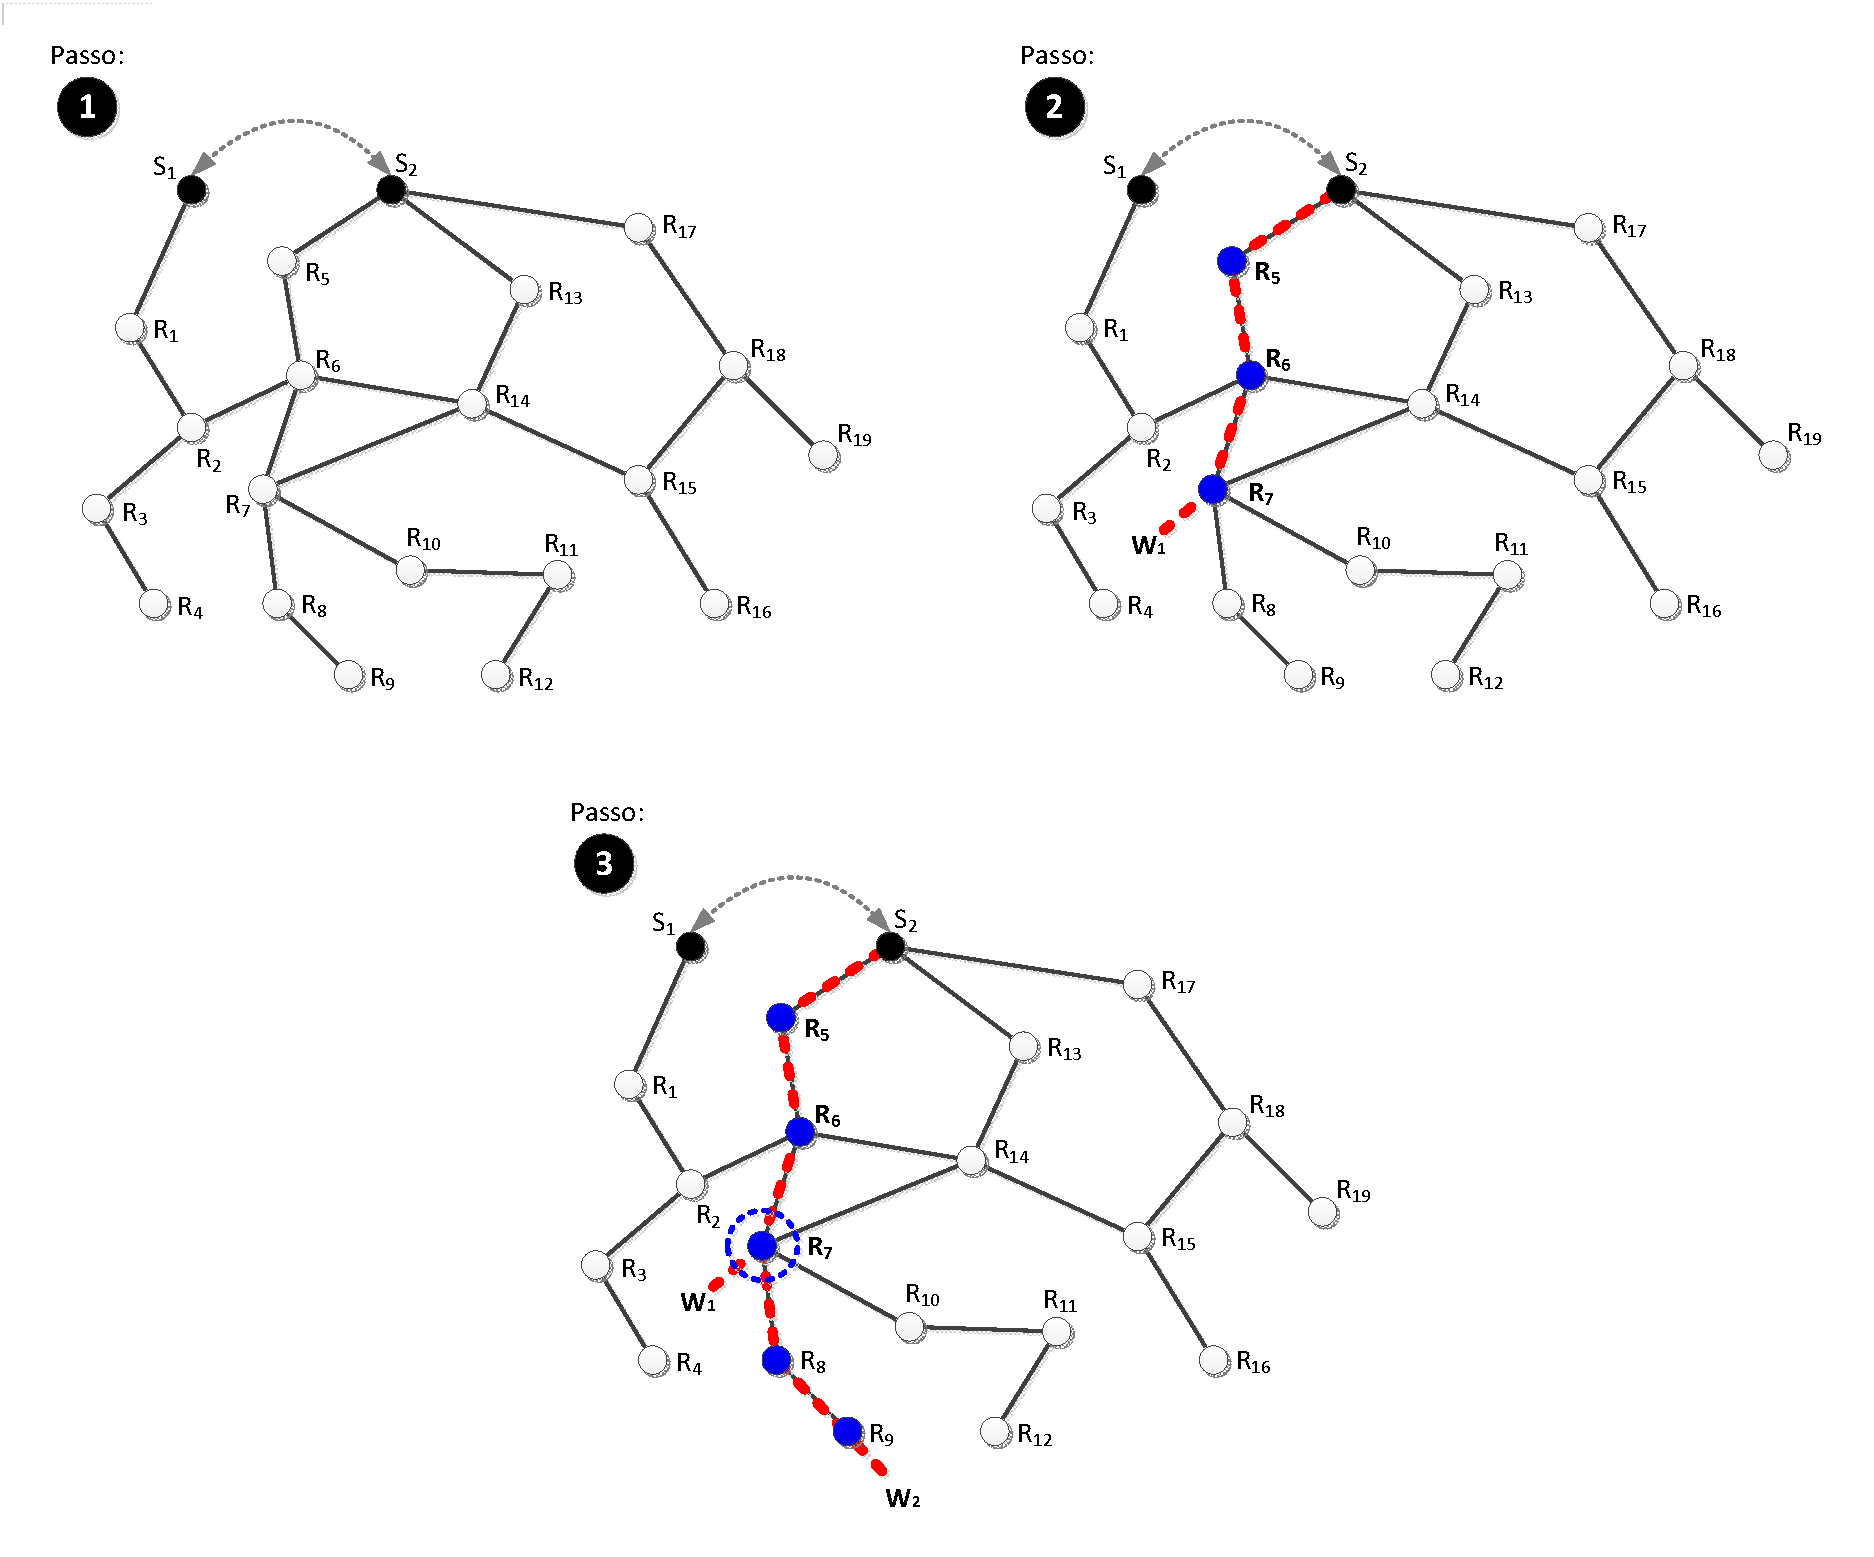
\includegraphics[scale=.5]{imgs/esquema-abstrato-formacao-parceria-intra.pdf}
\end{center}
\vspace{-0.8cm}
\caption{Cen�rio e passos para sele��o de n�s (exemplo 1).}
\label{fig:esquema-abstrato-formacao-parceria-intra}
\end{figure}

% $\{$\setwayiu{1}, \setwayiu{2}, $\dots$ \setwayiu{\setwayii}$\}$

Para entender detalhes desse processo, considere a Figura~\ref{fig:esquema-abstrato-formacao-parceria-intra}. No Passo 1, ilustra-se um cen�rio de rede \nets $=$ $G($\setservrepass, \setway$)$, onde \setservrepasss $=$ $\{$\servu{1}, \repassu{1..19}$\}$, \setways $=$ $\{\emptyset\}$ e \transmission $=$ $\{\{\emptyset\}$, $\{\emptyset\}$, $\{\emptyset\}\}$, ou seja, sem qualquer fluxo de dados \setpks sendo transmitido, tampouco nenhuma parceria efetivada e suprimindo-se os n�s \clis $\in$ \subsetcli$($\repassu{1..19}$)$. J� no Passo 2, ilustra-se a mesma rede \net, por�m com \transmission $=$ $\{\{$\servu{1}, \repassu{5..9}$\}$, \setpk, \subsetcli$($\repassu{9}$)\}$, constituindo-se o caminho \setwayiu{1} $=$ $\{$\servu{1}, ..., \repassu{9}$\}$ (linha tracejada e vermelha), portanto, \setway $=$ $\{$\setwayiu{1}$\}$ e \transmitqu{\repassu{9}} $=$ $1$. Nesse exemplo do Passo 2, o n� \repassu{9} recebe o fluxo de dados \setpks em modo \textit{unicast} e repassa \setpks para todos os n�s \clis $\in$ \subsetcli$($\repassu{9}$)$ em modo \textit{multicast}. Para constituir o caminho \setwayiu{1}, o n� \repassu{9} deve transmitir o pedido de registro de participa��o ao n� \servu{1} (como discutiu-se na Se��o~\ref{subsec:registro-participacao}) e, a partir de sua confirma��o,
processada pelo n� \servu{1} e enviada ao n� \repassu{9}, o n� \repassu{9} come�a a receber os pacotes \pks $\in$ \setpk. Com este procedimento, o n� \servu{1} passa a conhecer o caminho \setwayiu{1}, que pode ser utilizado para determinar futuras parcerias. Desse ponto em diante, utilizar-se-� tal exemplo como base para explicar outros aspectos do processo de forma��o de parceria do GMTP.

Na Figura~\ref{fig:esquema-abstrato-formacao-parceria-interseccao}, considera-se a forma��o de parceria por intersec��o do fluxo de dados \setpk, a partir do Passo 2 da Figura~\ref{fig:esquema-abstrato-formacao-parceria-intra}. Este procedimento ocorre quando um outro n� \repasss envia um pedido de registro de participa��o em dire��o ao n� \servu{1}, a fim de obter o fluxo de dados \setpk, motivado por algum n� \clis $\in$ \subsetcli$($\repass$)$. Nesse caso, se um n� \repasss transmitir um pedido de registro de participa��o atrav�s de um sub-caminho \setwayids tal que $\exists$\setwayis $\in$ \setway, o n� \servs determina a intersec��o de ambos e instrui o n� comum \ways a repassar o fluxo de dados \setpks tamb�m para \repass, sendo desnecessidade de enviar um segundo fluxo de dados na mesma dire��o de \setwayid. Sendo assim, a resposta de \servu{1} n�o resulta em uma nova transmiss�o do fluxo de dados \setpk, mas sim em uma mensagem de controle para o n� \way, ap�s identific�-lo como o n� comum a dois ou mais caminhos \setwayi. Isto implicar� que o referido n� \ways replique o fluxo de dados \setpk, mesmo quando $|$\subsetcli$($\way$)|$ $=$ $0$, mas de modo conveniente para evitar m�ltiplas transmiss�es do fluxo de dados \setpk, originadas em \serv. A fim de compreender o funcionamento desse procedimento, acompanhe a explica��o a seguir, com base na ilustra��o da Figura~\ref{fig:esquema-abstrato-formacao-parceria-interseccao} e no caminho \setwayiu{1}.

\begin{figure}
\begin{center}
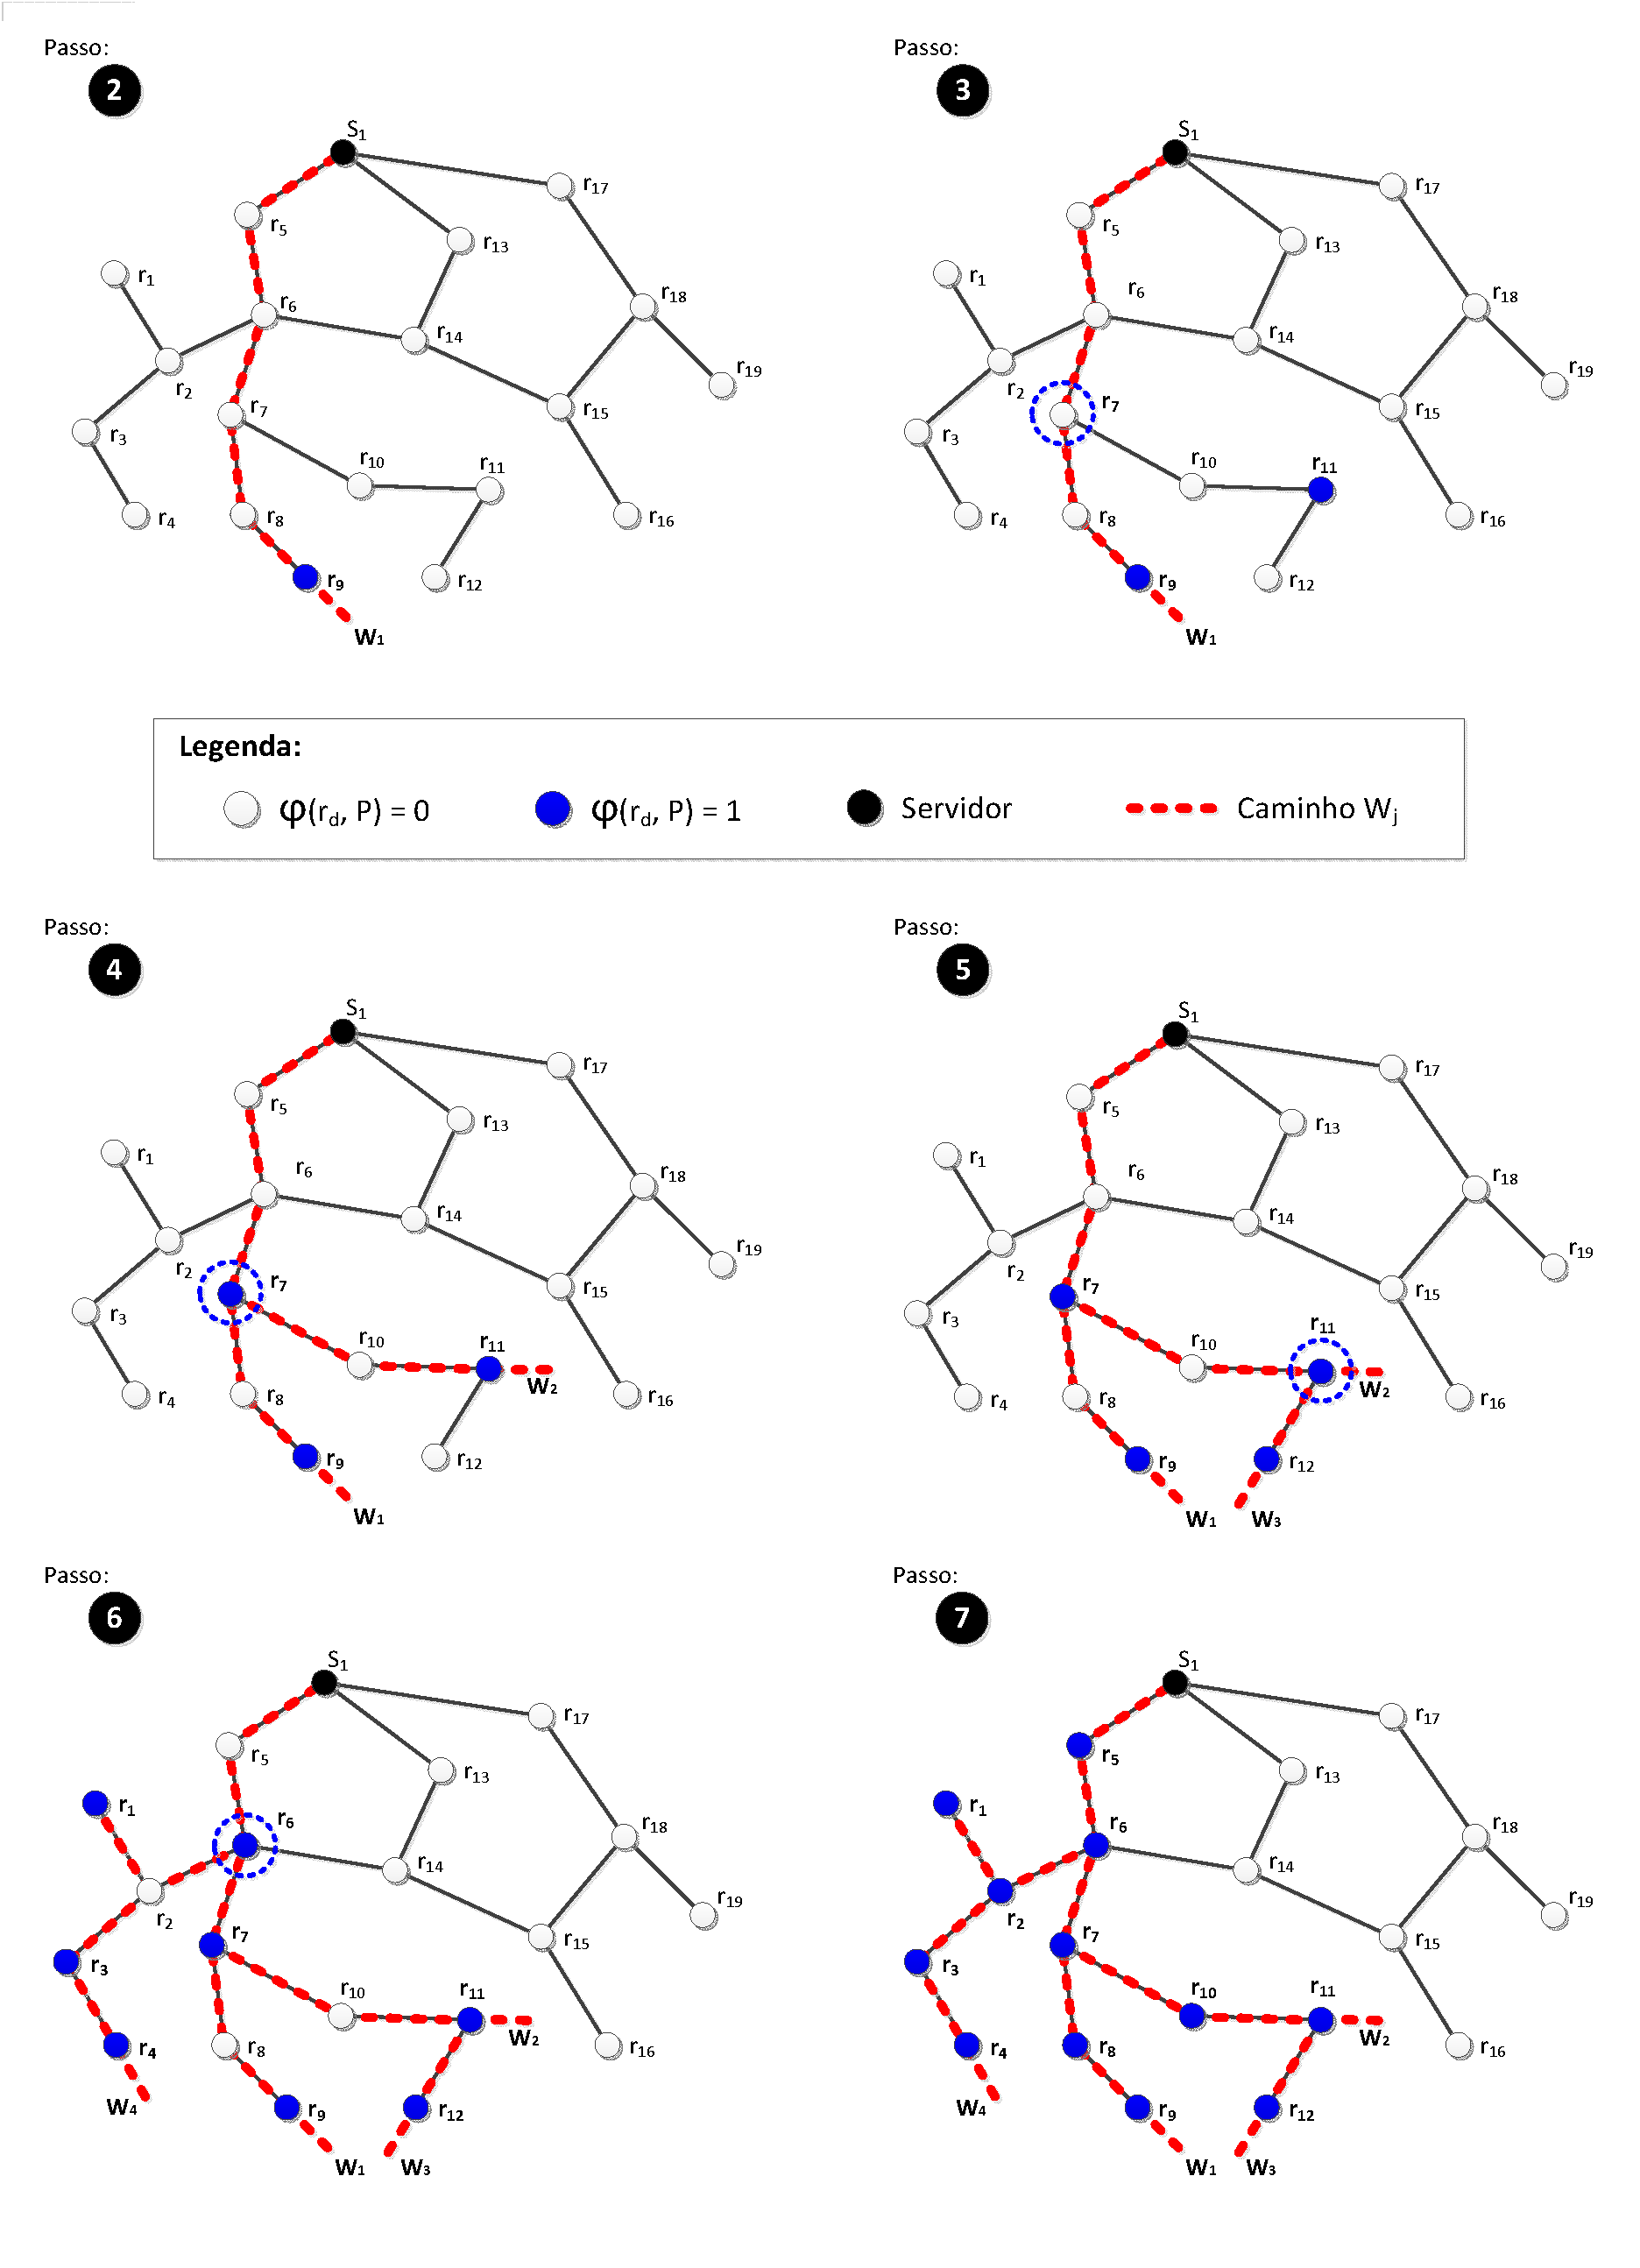
\includegraphics[scale=.5]{imgs/esquema-abstrato-formacao-parceria-interseccao.pdf}
\end{center}
\vspace{-0.8cm}
\caption{Cen�rio para sele��o de n�s por interse��o de caminhos \setwayi.}
\label{fig:esquema-abstrato-formacao-parceria-interseccao}
\end{figure}

Se qualquer um dos n�s \repassu{7,8,10,11,12}, suponha \repassu{11}, enviar um
registro de participa��o em dire��o � \servu{1} para obter um fluxo de dados
\setpks (Passo 3 da
Figura~\ref{fig:esquema-abstrato-formacao-parceria-interseccao}), o n�
\servu{1} descobrir� o caminho \setwayiu{2} $=$ $\{$\repassu{5}, \repassu{6},
\repassu{7}, \repassu{10}, \repassu{11}$\}$ (Passo 4). Em seguida, pela
intersec��o $($\setwayiu{1} $\cap$ \setwayiu{2}$)$, o n� \servu{1} determinar�
que o n� \repassu{7} � o n� comum e portanto instruir� que \repassu{7} repasse o
fluxo de dados \setpks tamb�m para o n� solicitante \repassu{11}. A instru��o de
\servu{1} para \repassu{7} deve determinar \transmitqu{\repassu{7}} $=$ $1$.
Em termos pr�ticos, isto obriga o n� \repassu{7} a adicionar uma nova entrada na
tabela de recep��o de fluxos de dados referente a \setpk, mesmo se
$|$\subsetcli$($\repassu{7}$)|$ $=$ $0$ para \setpk. � �bvio que, se
posteriormente $|$\subsetcli$($\repassu{7}$)|$ $>$ $0$ para \setpk, ser�
necess�rio apenas \repassu{7} criar um canal \textit{multicast} para a transmiss�o
local de \setpk, evitando-se um novo registro de participa��o em \servu{1}. Na
Se��o~\ref{subsec:conexao-requisicao}, discute-se em mais detalhes este aspecto
do GMTP, explicando-se os procedimentos de pedido de conex�o de um n� \cli.

Ao estender a discuss�o sobre o cen�rio ilustrado na
Figura~\ref{fig:esquema-abstrato-formacao-parceria-interseccao}, percebe-se que, se o n� \repassu{10} necessitar obter o mesmo fluxo de dados \setpk, seu pedido de registro de participa��o ser� interceptado pelo n� \repassu{7} e parte do procedimento supracitado se repete. Uma situa��o similar ocorre se o n� \repassu{12} ou qualquer n� \repasss $\in$ \setwayiu{4} tamb�m desejar obter o fluxo de dados \setpk, tal que \setwayiu{4} $=$ $\{$\repassu{1}, \repassu{2}, \repassu{3}, \repassu{4}$\}$ (Passo 5 e 6). Para o caso do n� \repassu{12}, o n� \repassu{11} interceptar� o pedido de registro de participa��o de \repassu{12}, ao passo que se for qualquer n� \repasss $\in$ \setwayiu{4}, o n� \repassu{6} realizar� tal intercepta��o, pois o n� \servu{1} determinar� \transmitqu{\repassu{6}} $=$ $1$, depois do primeiro pedido de registro de participa��o originado por qualquer n� \repasss $\in$ \setwayiu{4}. A �nica diferen�a nesses �ltimos casos � que, como \transmitqu{\repassu{7}} $=$ $1$ e \transmitqu{\repassu{11}} $=$ $1$, o n� \repassu{7} tem autonomia para responder ao n� \repassu{10} e ao n� \repassu{11} como se fosse o n� \servu{1}, sem repassar tal pedido em dire��o ao n� \servu{1}.

Para generalizar essa discuss�o sobre o processo de forma��o de parcerias do GMTP, caso existam outros n�s \repassu{q} interessados em obter um fluxo de dados \setpks e est�o interligados direto ou indiretamente a \repass, tal que \transmitqu{\repass} $=$ $1$, o n� \repasss sempre interceptar� o pedido de registro de participa��o dos n�s \repassu{q} e atuar� como se fosse o n� \servu{1}. No caso do exemplo que se discute, independente da ordem em que as requisi��es de registro de participa��o sejam enviadas por \ways $\in$ (\setwayiu{1} $\cup$ \setwayiu{2} $\cup$ \setwayiu{3} $\cup$ \setwayiu{4}), ser� necess�rio transmitir apenas um fluxo de dados \setpks para ``alimentar'' os quatro caminhos referidos. Isto significa que todos os n�s \clis $\in$ \subsetcli$($\setwayiu{1} $\cup$ \setwayiu{2} $\cup$ \setwayiu{3} $\cup$ \setwayiu{4}$)$ receber�o um �nico fluxo de dados, com repasse dos pacotes \pks $\in$ \setpks realizado em modo \textit{multicast} em cada sub-rede de cada n� \ways (Passo 7). Como a transmiss�o ser� em modo \textit{multicast}, torna-se indiferente a quantidade de n�s \clis desses caminhos, mas faz-se necess�rio um mecanismo para controle de congestionamento em modo \textit{multicast}, a ser discutido na Se��o~\ref{sec:ccgmtp}.

Note que, o n� \repasss que interceptar um pedido de conex�o para um fluxo de dados \setpk, deve transmitir para o n� \servs uma notifica��o sobre a(s) parceria(s) formada(s) por intersec��o. No caso do exemplo anterior, os n�s \repassu{6}, \repassu{7} e \repassu{11} devem realizar tal notifica��o enviando um pacote do tipo \pac{GMTP-Register}, como explicado na Se��o~\ref{subsec:registro-participacao}. Para isso, deve-se ativar o bit P (\textit{pass-along}) do cabe�alho GMTP (Figura~\ref{fig:gmtp-fixed-header}) para o pacote do tipo \pac{GMTP-Register}. Esta a��o � importante devido aos aspectos gerenciais de uma transmiss�o, onde uma aplica��o poder� contabilizar os n�s \repasss que est�o recebendo \setpk, mesmo que indiretamente, por meio da intercepta��o de registros de participa��o. A prop�sito, em ICN isso n�o � poss�vel.

Na pr�tica, n�o se faz necess�rio que o n� \repasss envie a notifica��o de intercep��o instantaneamente. Em vez disso, um n�s \repasss pode acumular diversos registros de participa��o durante um determinado intervalo de tempo e, em seguida, transmiti-los para o n� \serv. Como se trata de um aspecto em n�vel de implementa��o, tal decis�o est� fora do escopo dessa discuss�o. No caso da implementa��o do GMTP realizada em simulador e utilizada neste trabalho, definiu-se que para todo registro de participa��o interceptado, gera-se e transmite-se uma notifica��o ao n� \serv.

No Algoritmo~\ref{algo:findPartnerIntersectPath}, resumem-se os passos descritos anteriormente na perspectiva do n� \serv, a fim de determinar a forma��o de parcerias por intersec��o. Executa-se tal algoritmo quando o n� \servs recebe um pedido de registro de participa��o enviado por um n� \repasss para obter um fluxo de dados \setpk. Atrav�s dessa estrat�gia de forma��o de parceria, permitem-se repasses de pacotes de dados pelo nome do fluxo de dados e n�o com base no servidor que o produz e transmite. Em todo caso, o destino da requisi��o � sempre o servidor, garantindo-se que, se nenhum repassador interceptar o pedido de registro de participa��o, com certeza tal pedido alcan�ar� o servidor e o estabelecimento de conex�o ocorrer� normalmente. Por isso, � importante a continuidade do uso de endere�amento IP, ausente em redes ICN. Al�m disso, esta decis�o � fundamental para manter a compatibilidade com as aplica��es de rede existentes na Internet, que transmitem um pedido de conex�o e recebem uma resposta que pode ser ou n�o oficialmente gerada pelo servidor, mas o importante � receber o fluxo de dados \setpks -- o GMTP faz com que a rede cuide disso.

% O n� \servs compara os caminhos conhecidos
% \setwayis $\in$ \setways com o caminho \textit{\setwayiu{\repassconst_\repassi}}
% contido no pedido de conex�o transmitido por \repass. Se \servs encontrar um n�
% \ways em comum entre algum \setwayis e
% \textit{\setwayiu{\repassconst_\repassi}}, \servs instrui o n� \ways a
% interceptar os pr�ximos pedidos de registro de participa��o para obter \setpk;
% caso contr�rio, \servs aceita o novo pedido de conex�o, permitindo-se futuras
% parcerias por intersec��o. Note que, ap�s este procedimento, o n� \servs passa a
% conhecer o caminho \textit{\setwayiu{\repassconst_\repassi}}.

\begin{algorithm}[H]
\label{algo:findPartnerIntersectPath}
\SetAlgoLined
\caption{handleRegisterParticipation(\repass: PeerRelay, \pks $=$
\pac{GMTP-Register})}
\tcc{\servs executes this algorithm to finds the first node \ways common to a
known path \setwayis and the path \setwayiu{\repassconst_\repassi}. \setwayis is
already used for transporting \setpks to node in $\delta($\way, \setwayi$)$, and
\setwayiu{\repassconst_\repassi} contains all nodes between \repasss (requester)
and \serv. The packet \pks carries \setwayiu{\repassconst_\repassi} and the
\setpks flow name.}
\textit{done} \attrib \textit{false}\tcc*[r]{It becomes true when \ways is found}

\SetKwFunction{Union}{Union}\SetKwFunction{makePkt}{makePkt}
\SetKwFunction{Union}{Union}\SetKwFunction{getPacketFieldValue}{getPacketFieldValue}
\SetKwFunction{Union}{Union}\SetKwFunction{recvPktRdt}{recvPktRdt}
\SetKwFunction{Union}{Union}\SetKwFunction{sendPktRdt}{sendPktRdt}
\SetKwFunction{Union}{Union}\SetKwFunction{length}{length}
\SetKwFunction{Union}{Union}\SetKwFunction{getKnownPathsOfFlow}{getKnownPathsOfFlow}
\SetKwFunction{Union}{Union}\SetKwFunction{GMTPRegisterReply}{GMTPRegisterReply}

\textit{\setpk} \attrib \getPacketFieldValue{\pk, `flow'}\tcc*[r]{Extracts \setpks in \pk}
\textit{\setwayiu{\repassconst_\repassi}} \attrib \invert{\getPacketFieldValue{\pk, `path'}}\;
\textit{\setwayiu{\setpkc}} \attrib \getKnownPathsOfFlow{\setpk}\tcc*[r]{\setwayiu{\setpkc} $\subset$ \setway}
% \tcc*[r]{For a given flow and all the known paths \setways in this \serv, get a sub set of paths used to transmit \setpk}

\ForEach{\setwayis $\in$ \setwayiu{\setpkc}}{
    \ForEach{\ways $\in$ \setwayi} {
      \If(){\ways $\in$ \textit{\setwayiu{\repassconst_\repassi}}} {
        \tcc{The node \ways is common in \setwayis and in \textit{\setwayiu{\repassconst_\repassi}}.}
        \textit{done} \attrib \textit{true}\;
        break\;
      }
    }
    \If(){\textit{done}} {
% \tcc{Create a \pac{GMTP-Response} and send it to \way. After receiving \textit{\pk}, \ways becomes a relay of the flow \setpk.}
% \pks \attrib \makePkt{\pac{GMTP-Response}(1), \ways}\;
      \tcc{\servs stores \textit{\setwayiu{\repassconst_\repassi}} as a known path and replies to \repass, asking \ways to act as a relay for \setpk. \servs actives flag 'relay' of the \pac{GMTP-RegisterReply}.}
      \setwayiu{\setpkc}[\length{\setwayiu{\setpkc}}] \attrib \textit{\setwayiu{\repassconst_\repassi}}\;
      \Return{\GMTPRegisterReply{\way, relay=1}}\;
% \sendPktRdt(\pk)\;
% \exit{}\;
    }
}
\tcc{\servs must register \textit{\setwayiu{\repassconst_\repassi}} as a known path and reply to \repasss by accepting its connection request, since no node \ways is intersecting \textit{\setwayiu{\repassconst_\repassi}}. In this case, \servs starts the transmission of \pks $\in$ \setpks to \repass.}
\setway[\length{\setway}] \attrib \textit{\setwayiu{\repassconst_\repassi}}\;
\Return{\GMTPRegisterReply{\repass, relay=0}}\;
% \pks \attrib \makePkt{\pac{GMTP-Response}(0), \repass}\;
% \sendPktRdt(\pk)\;

\end{algorithm}
\vspace{0.8cm}

Com rela��o � praticidade do processo de forma��o de parcerias empregado no GMTP, um aspecto t�cnico muito importante deve ser ressaltado: apenas o n� \repasss que repassar \pks $\in$ \setpks para seus n�s \clis $\in$ \subsetcli$($\repass$)$ deve manter uma entrada sobre \setpks na tabela de recep��o de fluxos de dados, exceto quando sinalizado pelo n� \serv, como � o caso dos n�s \repassu{6} e \repassu{7} do exemplo anterior. Al�m disso, como a transmiss�o de um fluxo de dados \setpks entre um n� \repasss e seus n�s \clis $\in$ \subsetcli$($\repass$)$ ocorrer� sempre em modo \textit{multicast}, sendo necess�ria
apenas uma entrada na tabela de recep��o de fluxos de dados sobre \setpk. Com essa estrat�gia, espera-se permitir uma quantidade significativa de n�s \clis capazes de reproduzir um fluxo de dados \setpk, sem sobrecarregar a rede com demasiadas transmiss�es do mesmo fluxo de dados \setpk, al�m de reduzir o tempo de inicializa��o para reproduzir o fluxo de dados \setpks e o �ndice de continuidade para um fluxo de dados \setpk. Ademais, apresentaram-se procedimentos que n�o s�o adotados em nenhum protocolo de rede pesquisado no estado da arte. Trata-se da primeira solu��o em que o servidor auxilia os roteadores no processo de forma��o de parcerias, delegando-se para estes a responsabilidade de distribuir um determinado fluxo de dados \setpk, tudo de forma transparente para as aplica��es. Como resultado, pode-se afirmar que os roteadores passam a funcionar como se fossem servidores de uma CDN, s� que participando dinamicamente sempre que conveniente.

Por fim, um outro aspecto no processo de forma��o de parcerias do GMTP � o uso de informa��es sobre a capacidade de transmiss�o de um caminho \setwayis para determinar as parcerias entre os n�s \repass, bem como a qualidade do fluxo de dados a ser transmitido pelo servidor. Diferentemente se comparado �s solu��es baseadas em HTTP (por exemplo, DASH), em vez de um servidor GMTP gerar m�ltiplos fluxos de dados, codificados em diferentes taxas de bits, gera-se o fluxo de dados com a taxa de bits correspondente � capacidade m�xima de transmiss�o do caminho \setwayis em um determinado instante. Isto ocorre porque o GMTP exp�e, ao n� \serv, a informa��o de controle de congestionamento percebida pelos n�s \ways $\in$ \setwayi. Sendo assim, o n� \servs  codifica a m�dia em uma qualidade poss�vel de ser transportada atrav�s de \setwayis utilizando um codificador do tipo VBR (\textit{Variable Bit Rate}), como o H.264~\cite{6422289}. Na Se��o~\ref{subsec:mudccp-ucc}, discute-se essa fun��o em mais detalhes.

% \subsubsection{\space\space\space\space\space\space2. Forma��o de parcerias por
% intersec��o de \setwayi}
% \label{subsec:parcintersec}

% \subsubsection{\space\space\space\space\space\space3. Forma��o de parcerias por
% combina��o de \setwayi}
% \label{subsec:parccombina}
%
% O procedimento de forma��o de parcerias por combina��o considera um n�
% \textit{pivot} \servs e consiste em combinar caminhos distintos \setwayiu{1} e
% \setwayiu{2}, tal que \setwayiu{1} $\cap$ \setwayiu{2} $= \{$\serv$\}$, como
% ilustra-se na Figura~\ref{fig:esquema-abstrato-formacao-parceria-combinacao},
% Passo 1. Dessa forma, dado um conjunto de caminhos conhecidos \setway, o n�
% \servs executa as combina��es e instrui, por exemplo, dois n�s \wayu{1} $\in$
% \setwayiu{1} e \wayu{2} $\in$ \setwayiu{2} a se tornarem parceiros para
% compartilharem o mesmo fluxo de dados \setpk, transmitindo apenas um fluxo de
% dados \setpks para ser distribu�dos aos n�s \clis $\in$
% $($\subsetcli$($\wayu{1}$)$ $\cup$ \subsetcli$($\wayu{2}$))$. Este procedimento
% resultar� na constitui��o de um caminho \setwayis contendo todos os n�s \repasss
% entre os \wayu{1} e \wayu{2}. Como consequ�ncia, pode-se repassar o mesmo fluxo
% \setpks tamb�m para outros n�s \clis $\in$ \subsetcli$($\repass$)$.
%
% \begin{figure}[ht]
% \begin{center}
% \includegraphics[scale=.5]{imgs/esquema-abstrato-formacao-parceria-combinacao.pdf}
% \end{center}
% \vspace{-0.8cm}
% \caption{Cen�rio e passos para sele��o de n�s por combina��o de caminhos
% \setwayi.}
% \label{fig:esquema-abstrato-formacao-parceria-combinacao}
% \end{figure}
%
% % Tal procedimento pode ajudar os n�s \repasss a expandirem
% % suas parcerias, incluindo a possibilidade de obter pacotes de dados \pks $\in$
% % \setpks de m�ltiplos n�s parceiros \repassu{q}.
%
% Com o registro de participa��o de cada n� \repasss em \serv, o n� \servs
% conhece os caminhos \setwayis $\subset$ \setways atrav�s dos quais se
% transmite o fluxos de dados \setpk. Sendo assim, \servs pode determinar
% candidados a parceiros \repassu{q} de um determinado n� \repasss e esse
% procedimento acontece da seguinte forma. Um n� \repasss enviar uma mensagem ao
% n� \servs para solicitando a lista de parceiros
%
% Para isso, o n�
% \servs instrui
% os n�s \wayu{1} e \wayu{2} a executarem um algoritmo para determinar se
% \wayu{1} servir� \wayu{2} ou se \wayu{2} servir� \wayu{1}. Note que � poss�vel
% que a parceria entre \wayu{1} e \wayu{2} n�o ocorra. Por exemplo, \wayu{1} se
% tornar� parceiros de \wayu{2} apenas se o custo entre \wayu{1} e \wayu{2} for
% menor do que o custo entre \wayu{1} e \serv.
%
%  a
% execu��o da forma��o de parceria por combina��o, o n� \servs envia um pacote do
% tipo \pac{GMTP-Partnership} aos n�s \repass, escolhidos dentre os que est�o
% conectados e recebendo o fluxo de dados \setpks diretamente de \serv, para
% executarem o Algoritmo~\ref{algo:findPartnerCombinePath}. Em geral funciona com
% base em busca bin�ria, tendo como crit�rio o custo entre $\zeta($\setwayiu{1}$)$
% e $\zeta($\setwayiu{2}$)$  da seguinte forma. O n� \servu{2} processa os
% caminhos
% \setwayis conhecidos e determina quais s�o os melhores parceiros \repassu{q}
% para um determinado n� \repass, sendo tal informa��o enviada para \repass. No
% caso do cen�rio ilustrado na
% Figura~\ref{fig:esquema-abstrato-formacao-parceria-combinacao}, Passo 2, �
% poss�vel combinar os caminhos \setwayiu{1} e \setwayiu{2} pelos n�s \repassu{6}
% e o \repassu{15}. Ao combinar dois caminhos \setwayiu{1} e \setwayiu{2}, sempre
% haver� duas dire��es para a transmiss�o do fluxo de dados \setpk, uma ilustrada
% no Passos 3 e outra ilustrada no Passo 4 da
% Figura~\ref{fig:esquema-abstrato-formacao-parceria-combinacao}. Para decidir
% qual op��o escolher, o n� \servu{2} compara os custos $\zeta($\setwayiu{1}$)$ e
% $\zeta($\setwayiu{2}$)$. Se $\zeta($\setwayiu{1}$) \geq \zeta($\setwayiu{2}$)$,
% ent�o o n� \servu{2} solicita que \repassu{9} envie um pedido de conex�o para
% \repassu{16} (Passo 4). Por fim, o n� \repassu{15} deve enviar uma notifica��o
% para o n� \servu{2} informando sobre a constitui��o do novo caminho \setwayi. Em
% caso de $\zeta($\setwayiu{1}$) \leq \zeta($\setwayiu{2}$)$, ent�o o n� \servu{2}
% solicitar� que \repassu{16} envie um pedido de conex�o para \repassu{9} (Passo
% 3), ao passo que o restante do procedimento ocorrer� de forma similar ao que
% acabara de ser explicado.
%
% Esta � a grande motiva��o da forma��o de parceria por combina��o, pois quando o
% pedido de conex�o do n� \repassu{9} alcan�ar o n� \repassu{15}, este o
% interceptar� e, nesse instante, constitui-se um novo caminho \setwayis $=
% \{$\repassu{15}$,$\repassu{14}$,$\repassu{6}$,$\repassu{7}$,$\repassu{8}$,
% $\repassu{9}$\}$.
%
% � importante salientar que o pedido de conex�o enviado pelo n� \repassu{9}
% para o n� \repassu{15} deve conter uma sinaliza��o (\textit{flag}) que
% instruir� o n� \repassu{6} a n�o interceptar tal pedido de conex�o. Para
% tal sinaliza��o, d�-se o nome de \textit{ignorar pedido de conex�o},
% do ingl�s \textit{bypass connection request}.
%
% Nessa estrat�gia de forma��o de parceria, permite-se que um n� \repasss obtenha
% os pacotes \pks $\in$ \setpks de duas ou mais fontes distintas. No caso do
% exemplo supracitado, o n� \repassu{6} pode continuar recebendo o fluxo de dados
% atrav�s do caminho \setwayiu{1} e tamb�m atrav�s do novo caminho \setwayis que
% acabara de ser constitu�do.
%
% Nesse contexto, para realizar a forma��o de parceria por combina��o, o n� \servs
% executa o Algoritmo~\ref{algo:findPartnerCombinePath}.\\
%
% \begin{algorithm}[H]
% \label{algo:findPartnerCombinePath}
% \SetAlgoLined
% \KwData{\textit{relayPartners} \attrib [ ]}
%
% \SetKwFunction{Union}{Union}\SetKwFunction{make_pkt}{make\_pkt}
% \SetKwFunction{Union}{Union}\SetKwFunction{recv_pkt_rdt}{recv\_pkt\_rdt}
% \SetKwFunction{Union}{Union}\SetKwFunction{send_pkt_rdt}{send\_pkt\_rdt}
% \SetKwFunction{Union}{Union}\SetKwFunction{getKnownPaths}{getKnownPaths}
% \SetKwFunction{Union}{Union}\SetKwFunction{matchSimilarPath}{matchSimilarPath}
% \SetKwFunction{Union}{Union}\SetKwFunction{parse_path}{parse\_path}
% \SetKwFunction{Union}{Union}\SetKwFunction{length}{length}
%
% mspf \attrib 0.4\tcc*[r]{paths are considered similar if similarity level is
% equal or above mspf value}
% pathSet \attrib \getKnownPaths{}\tcc*[r]{get \setways known in this \serv}
%
% \ForEach{\setwayiu{x} $\in$ \setway}{
%   \If(){\matchSimilarPath{\setwayiu{x}, \setwayis} >= mspf}{
%     \tcc{Get the closest partner in the path (intersection between \setwayiu{x}
% and \setwayi) and add to the list of prospective partners for \repass.}
%
%     prosRelay = NULL\;
%     \ForEach{\ways $\in$ \setwayiu{x}} {
%       \If(){\ways $\in$ \setwayi} {
% 	\textit{relayPartners}[\length{relayPartners}] \attrib prosRelay\;
%       }
%     }
%   }
% }
%
% pkt $ \leftarrow$ make\_pkt(GMTP\_ADV\_RELAY(\textit{relayPartners}), \repass)\;
%
% send\_pkt\_rdt(pkt)\;
%
% \caption[matchPartnersByPathCombination(\setwayi,
% \repass)]{matchPartnersByPathCombination(\setwayi, \repass)}
% \end{algorithm}
% \vspace{0.8cm}

\section{Transmiss�o de \pks $\in$ \setpks atrav�s de \net}
\label{sec:asptransrecep}

No GMTP, transmite-se os pacotes de dados \pks $\in$ \setpks utilizando uma estrat�gia h�brida \textit{push/pull}. Utiliza-se o m�todo \textit{push} por padr�o, onde os n�s \servs iniciam a transmiss�o de \pks $\in$ \setpks para os demais n�s \ways $\in$ \setwayi. J� o m�todo \textit{pull} � utilizado somente quando um n� \clis $\in$ \setclis precisa obter parte de uma m�dia que est� na imin�ncia de ser reproduzida e ainda n�o foi repassada por um n� \repasss via \textit{push}, de acordo com o seu mapa de \textit{buffer}.

% Os n�s \repasss mant�m um mapas de
% \textit{buffer}, sendo que um no \repasss sempre ter� um mapa de \textit{buffer}
% mais atualizado do que os mapas de \textit{buffer} dos n�s \clis $\in$
% \subsetcli$($\repass$)$.

Nessa se��o, apresentam-se detalhes sobre como se realiza a dissemina��o de pacotes de dados \pks $\in$ \setpks e como os n�s \clis recebem tal conte�do para reprodu��o, discutindo-se aspectos sobre indexa��o, requisi��o, recep��o e compartilhamento de um fluxo de dados \setpk.

\subsection{Indexa��o de \setpk}
\label{subsec:content-index}

No GMTP, um fluxo de dados \setpks tem um nome �nico que o identifica em qualquer n�. Na pr�tica, cada fluxo de dados \setpks corresponde a uma m�dia gerada a partir de um evento ao vivo \event, por exemplo, a transmiss�o de um jogo de futebol, corrida de f�rmula 1, etc.

Define-se um nome de um fluxo de dados \setpks por um c�digo de \textit{hash} MD5 no formato UUID (\textit{Universally Unique IDentifier}) de \ut{128}{bits}~\cite{RFC4122}. Na sua forma can�nica, representa-se \setpks por uma sequ�ncia de 32 d�gitos hexadecimal, exibidos em cinco grupos separados por h�fen, na forma de \{8\}-\{4\}-\{4\}-\{4\}-\{12\}. Por exemplo, \setpks $=$ \textit{641f931f-d3ac-50e3-b625-537574541f1f}.

Na pr�tica, para gerar o nome para um fluxo de dados \setpk, utiliza-se uma fun��o de \textit{hash} do tipo MD5. Sendo assim, para determinar o nome de um fluxo de dados \setpk, disponibilizado por um n� \serv, utiliza-se MD5(IP$_{\servconst_\servi}$ + : + PORTA$_{\servconst_\servi}$). Por exemplo, suponha que um servidor esteja disponibilizando um fluxo de dados \setpks atrav�s do endere�o 200.17.113.98, na porta 21200. O nome do fluxo de dados \setpks ser� definido por \textit{MD5("200.17.113.98:21200") = f8ea01fd-4d71-5d95-89ec-35646e11d7fe}. 

Opcionalmente, o n� \servs pode divulgar o nome do fluxo de dados atrav�s do servi�o DNS. J� com rela��o ao t�tulo do conte�do e sua descri��o, tais informa��es podem ser divulgadas por meio de um servi�o web, ou por meio de uma busca de diret�rio via um \textit{Web Services}. Independente da forma que o n� \servs disponibilize os nomes dos fluxos de dados \setpk, de posse de um identificador de um fluxo de dados \setpk, um n� GMTP poder� solicitar os pacotes de dados \pks $\in$ \setpk. Al�m disso, os n�s \repasss mant�m a tabela de recep��o dos fluxo de dados que est�o repassando para os n�s \clis $\in$ \subsetcli$($\repass$)$ e, sendo assim, podem compartilh�-la para outros repassadores. Atualmente, n�o se explora o compartilhamento da tabela de repasse, mas pode ser feito para formar parcerias entre dois n�s \repasss sem precisar consultar o n� \serv, por exemplo. Com esse esquema de nomes baseado no endere�o IP e porta, o GMTP n�o requer altera��es na camada de aplica��o para informar o fluxo de dados de interesse -- a aplica��o continua informando endere�o IP e n�mero da porta no momento do estabelecimento de uma conex�o, mantendo-se a compatibilidade com as aplica��es existentes e, portanto, futuras ado��o do GMTP na Internet.

No caso do uso do DNS, o n� \servs divulga os identificadores de todos os eventos sendo transmitido por meio de um mecanismo de atualiza��o din�mica de registro de DNS, como especificado na RFC 2136~\cite{RFC2136}. Para o GMTP, criou-se um novo tipo de registro de DNS chamado de SID (\textit{Streaming IDentifier}).

No Quadro~\ref{algo:requestDNS}, ilustra-se um exemplo de uma requisi��o DNS, utilizando a ferramenta \textit{dig}, um comando de terminal para Linux. Nesse exemplo, apresenta-se a lista dos nomes dos fluxos de dados transmitidos pelo dom�nio administrativo \textit{globo.com}. Por ser uma consulta simples de DNS, qualquer sistema final conectado � Internet pode realizar tal procedimento, enaltecendo-se a facilitar de adaptar aplica��es multim�dia existentes para utilizar o GMTP. Ao indexar o conte�do atrav�s de um servi�o de DNS, permite-se desacoplar a forma de indexar um determinado conte�do e a forma de obt�-lo, que passa a ser de responsabilidade da infraestrutura de rede e n�o de uma ou mais aplica��es isoladamente, como nas solu��es apresentadas no Cap�tulo~\ref{cap:trabalhosrelacionados}. Isto pode permitir o aumento das aplica��es multim�dia sem se preocupar como localizar um determinado conte�do, extrapolando-se as barreiras administrativas de cada sistema de gera��o de conte�dos multim�dia, bastando para isso apenas todas as aplica��es utilizarem o protocolo GMTP. Consequentemente, um fluxo de dados \setpk, gerado por uma aplica��o qualquer APL1, em execu��o em um n� \serv, poder� ser reproduzido por uma aplica��o APL2, em execu��o em um n� \cli, independentemente de seus fornecedores (por exemplo, similar ao servi�o Web, onde as aplica��es servidoras, como o Apache, � independente das aplica��es cliente, como Chrome, Firefox, etc). Para que essa vis�o seja empregada, definiu-se uma fun��o para descrever a m�dia transmitida em um fluxo de dados \setpk.

\vspace{0.5cm}

\newcommand{\bigspace}{~~~~~}

\begin{algorithm}[H]
\label{algo:requestDNS}
\SetAlgoLined
\SetAlgorithmName{Quadro}{quadro}{.}

\caption{Exemplo de requisi��o e resposta da lista de nomes dos fluxos de dados
\setpks de um distribuidor de conte�dos multim�dia.}

\textbf{dig} -t SID globo.com\tcc*[r]{comando de requisi��o}
\textbf{QUESTION SECTION:}\\
\bigspace globo.com.\bigspace IN\bigspace SID\\

\textbf{ANSWER SECTION:}\\
\bigspace globo.com.\bigspace IN\bigspace SID\bigspace
"111f931f-d3ac-10e3-b62f-f17f74541f1f"\\
\bigspace globo.com.\bigspace IN\bigspace SID\bigspace
"72c44591-7d82-427c-825f-722f015787c1"\\
\bigspace globo.com.\bigspace IN\bigspace SID\bigspace
"0bb0b9f5-f57d-4da5-8a6c-13acf1965188"\\

\textbf{SUMMARY:}\\
\bigspace Query time: 4 msec\\
\bigspace SERVER: 192.168.1.252:53(192.168.1.252)\\
\bigspace WHEN: Tue Jul 16 15:44:25 2013\\

\end{algorithm}
\vspace{0.8cm}

\subsection{Descri��o de um fluxo de dados \setpk:}
\label{subsubsec:desc-conteudo}

O GMTP permite nativamente a descri��o da m�dia a ser transmitida e com isso promover a compatibilidade entre diferentes aplica��es. Para isto, incorporou-se ao GMTP o protocolo o SDP (\textit{Session Description Protocol}), definido na RFC 2327~\cite{RFC2327}. Com o SDP, permite-se que as aplica��es obtenham mais detalhes sobre a m�dia, flexibilizando-se o acesso a um determinado conte�do. Como consequ�ncia, as aplica��es se preocupam apenas com a decodifica��o e a reprodu��o do conte�do ao usu�rio, independente de qual sistema remoto que o gerou.

Com esta decis�o, torna-se mais f�cil implementar novas aplica��es multim�dia, ao passo que fica mais f�cil adaptar aplica��es existentes para fazer uso do GMTP, uma vez que, em sua grande maioria, j� se utiliza o SDP. Do ponto de vista de engenharia de software, isto evitar� a repeti��o de esfor�o com implementa��es j� consolidadas e que, com o passar dos anos, provou-se funcionar a contento, como foi o caso do SDP. Consequentemente, caso seja necess�rio a atualiza��o do referido padr�o, tal atualiza��o ser� realizada internamente no GMTP e todas as aplica��es automaticamente j� poder�o usufruir dos novos recursos disponibilizados. Na pr�tica, isto significa uma atualiza��o em n�vel de sistema operacional. A t�tulo comparativo, considerando os protocolos baseado em HTTP e os sistemas de distribui��o multim�dia, descritos no Cap�tulo~\ref{cap:trabalhosrelacionados}, cada um possui uma proposta diferente de descri��o da m�dia, predominando o uso de XML, por�m n�o se mantendo o mesmo formato. A consequ�ncia disso � que a aplica��o cliente, para suportar diversos sistemas, ter� que implementar cada uma dessas propostas e usar XML gasta-se mais espa�o se comparado ao SDP.

Para uma aplica��o em execu��o em \serv, faz-se necess�rio apenas determinar as informa��es da m�dia e as fornece ao GMTP atrav�s de passagem de par�metro via \textit{socket}. Em seguida, o GMTP fica pronto para enviar a descri��o da m�dia como resposta ao pedido de conex�o, dentro do campo de dados do pacote do tipo \pac{GMTP-Register-Reply} ou \pac{GMTP-MediaDesc}. Como um n� \repasss pode interceptar um pedido de conex�o, o n� \repasss tamb�m pode transmitir a descri��o da m�dia aos seus n�s parceiros \repassu{q}. Al�m disso, um n� \repass, ao interceptar uma solicita��o por uma m�dia para atender a um pedido de um n� \repassu{q}, decide qual fluxo de dados deve ser transmitido, com base na taxa de transmiss�o observada entre \repasss e \repassu{q} e na disponibilidade de codifica��o da m�dia gerada pelo n� \serv. No Quadro~\ref{algo:sdp-mediadesc}, apresenta-se um exemplo de uma mensagem SDP e, a seguir, descreve-se cada um dos poss�veis atributos de uma mensagem SDP.

\begin{itemize}

  \item \textit{v}, a vers�o do SDP;

  \item \textit{o}, a lista de n�s \servs que a distribui;

  \item \textit{s}, o nome da m�dia, como discutido na
Se��o~\ref{subsec:content-index};

  \item \textit{i}, o t�tulo da m�dia;

  \item \textit{u}, a URI que descreve detalhes sobre a m�dia;

  \item \textit{c}, as informa��es de conex�o, como a vers�o do protocolo de
rede e o endere�o do n� \repass;

  \item \textit{f}, o certificado digital emitido pelo n� \servs para
verifica��o
de autenticidade dos pacotes \pks $\in$ \setpks (opcional). Este assunto
ser� retomado na Se��o~\ref{sec:seguranca};

  \item \textit{m}, o tipo da m�dia, a porta de conex�o e protocolo de
transporte; e

  \item \textit{a}, atributos adicionais sobre a m�dia como, por exemplo,
qualidade, idioma, taxa de bits m�nima e m�xima necess�ria para transmitir a
m�dia, em bytes.

\end{itemize}

\vspace{0.5cm}

\begin{algorithm}[H]
\label{algo:sdp-mediadesc}
\SetAlgoLined
\SetAlgorithmName{Quadro}{quadro}{.}

\bigspace v=0\\
\bigspace o=- IN IP4 177.135.177.241, IP4 186.192.82.163, IP6 2001:0db8:85a3::7344\\
\bigspace m=video 51372 GMTP/RTP/MPEG-4.2 256 pt-br\\
\label{line:sdp-mediadesc:m1}
\bigspace m=video 51373 GMTP/RTP/MPEG-4.2 512 pt-br\\
\bigspace m=video 51374 GMTP/RTP/MPEG-4.2 1024 pt-br\\
\bigspace m=video 51375 GMTP/RTP/MPEG-4.2 2048 pt-br\\
\bigspace m=video 51376 GMTP/RTP/MPEG-4.2 4096 pt-br\\
\label{line:sdp-mediadesc:m5}
\bigspace s=72c44591-7d82-427c-825f-722f015787c1\tcc*[r]{ver
Se��o~\ref{subsec:content-index}}
\label{line:sdp-mediadesc:index}
\bigspace i=An Introduction about Global Media Transmission Protocol (GMTP).\\
\label{line:sdp-mediadesc:title}
\bigspace u=http://www.ic.ufal.br/projects/gmtp/introduction.ps\\
\label{line:sdp-mediadesc:desc}
% \bigspace c=IN IP4 200.17.113.100\\
\bigspace f=x509:http://177.135.177.241/certs/cert.crt\tcc*[f]{ver Se��o~\ref{sec:seguranca}}\\
\label{line:sdp-mediadesc:f}

\caption{Exemplo de uma mensagem SDP no pacote \pac{GMTP-MediaDesc}.}
\end{algorithm}
\vspace{0.8cm}

No exemplo apresentado no Quadro~\ref{algo:sdp-mediadesc}, Linha 1, define-se o uso da vers�o 1.0 do protocolo SDP. Na Linha 2, descreve-se que a m�dia correspondente a \setpks est� dispon�vel atrav�s de tr�s n�s \servs que constituem a rede CDN, os quais dois s�o acess�veis atrav�s de endere�os IPv4 e um atrav�s de um endere�o IPv6. Entre as Linhas~\ref{line:sdp-mediadesc:m1} e~\ref{line:sdp-mediadesc:m5}, descreve-se que o primeiro n� \serv, especificado na Linha 2, transmite \setpks codificado em cinco taxas de bits (\ut{256}{Kbps}, \ut{512}{Kbps}, \ut{1024}{Kbps}, \ut{2048}{Kbps} e \ut{4096}{Kbps}) e com a por��o do �udio no idioma \textit{portugues/brasil}. Cada fluxo de dados correspondente � uma determinada codifica��o de bits � acess�vel atrav�s de uma porta diferente em \servs e, dessa forma, pode-se permitir m�ltiplas codifica��es da m�dia e com diferentes formatos e idiomas (caso a organiza��o do evento ofere�a o servi�o de tradu��o simult�nea). Por exemplo, o primeiro fluxo de dados (Linha~\ref{line:sdp-mediadesc:m1}) est� codificado no formato MPEG-4 (Parte 2), com uma taxa de bits de \ut{256}{Kbps} e acess�vel atrav�s da porta $51372$. Em seguida, na Linha~\ref{line:sdp-mediadesc:index}, especifica-se o nome da m�dia e nas Linhas~\ref{line:sdp-mediadesc:title} e~\ref{line:sdp-mediadesc:desc}, especificam-se o t�tulo do evento e uma URL para maiores informa��es. Por fim, na Linha~\ref{line:sdp-mediadesc:f}, observa-se uma URL do certificado digital, a ser utilizado pelos n�s \repasss para verificar a autenticidade do conte�do de pacote de dados \pks $\in$ \setpk. Na Se��o~\ref{sec:seguranca}, discute-se este �ltimo assunto em mais detalhes.

� importante salientar que os n�s \repasss utilizam as informa��es da taxa de bits para determinar o tamanho do \textit{buffer} de recep��o necess�rio para comportar os pacotes de dados \pks $\in$ \setpks, sendo adicionada uma entrada na tabela de recep��o de fluxos de dados para cada fluxo codificado em uma taxa de bit.

% Al�m
% disso, o tamanho do \textit{buffer} � definido em conson�ncia com os par�metros
% determinados pelo algoritmo de controle de congestionamento executado no m�dulo
% GMTP-Inter, a ser discutido em detalhes na
% Se��o~\ref{sec:ccgmtp}, a seguir.

\subsection{Estabelecimento de conex�o entre \clis e \servs para obter \setpk}
\label{subsec:conexao-requisicao}

Divide-se o processo de estabelecimento de conex�o em tr�s fases. A Fase 1 acontece quando, por exemplo, um n� qualquer \cliu{1} $\in$ \subsetcli$($\repass$)$ deseja obter \setpks transmitido por um n� \servu{1} e n�o existe nenhum outro n� \clis $\in$ \subsetcli$($\repass$)$ em sua rede local recebendo \setpk. J� a Fase 2 acontece quando um outro n� \cliu{2} $\in$ \subsetcli$($\repass$)$ precisa obter o mesmo fluxo de dados \setpk, solicitado previamente pelo n� \cliu{1}. E, por fim, a Fase 3 acontece quando o n� \repasss come�a a buscar novos n�s parceiros \repassu{q} a fim de obter \setpk. Na Figura~\ref{fig:processo-conexao}, ilustram-se doze n�s \repass, que constituem uma rede de diferentes dom�nios administrativos, sendo o n� \repassu{1} o repassador de um desses dom�nios, composto por 6 n�s \clis $\in$ \subsetcli$($\repassu{1}$)$ (Rede Local), e um n� \serv, que gera o fluxo de dados \setpk.

\begin{figure}[ht]
\begin{center}
\includegraphics[scale=.7]{imgs/processo-conexao.pdf}
\end{center}
\vspace{-1cm}
\caption{Exemplo de rede para o estabelecimento de conex�o do \mudccp.}
\label{fig:processo-conexao}
\end{figure}

A regra geral � que um n� \repasss deve consultar a tabela de recep��o de fluxo de dados (Se��o~\ref{subsec:tabela-recepcao}) todas as vezes que processar um pacote do tipo \pac{GMTP-Request} ou do tipo \pac{GMTP-Register}. Com base no estado da referida tabela, que define a fase de conex�o para um determinado fluxo de dados \setpks solicitado, o n� \repasss realiza uma determinada a��o de registro de participa��o e repasse.

\subsection{Fase 1: primeira requisi��o a um fluxo de dados \setpk}
\label{subsec:conn-fase1}

A Fase 1 ocorre quando nenhum n� \clis $\in$ \subsetcli$($\repass$)$ est� recebendo um fluxo de dados \setpk. Com base na Figura~\ref{fig:processo-conexao-1}, onde ilustra-se um exemplo de conex�o na Fase 1, considere:

\begin{figure}[ht]
\begin{center}
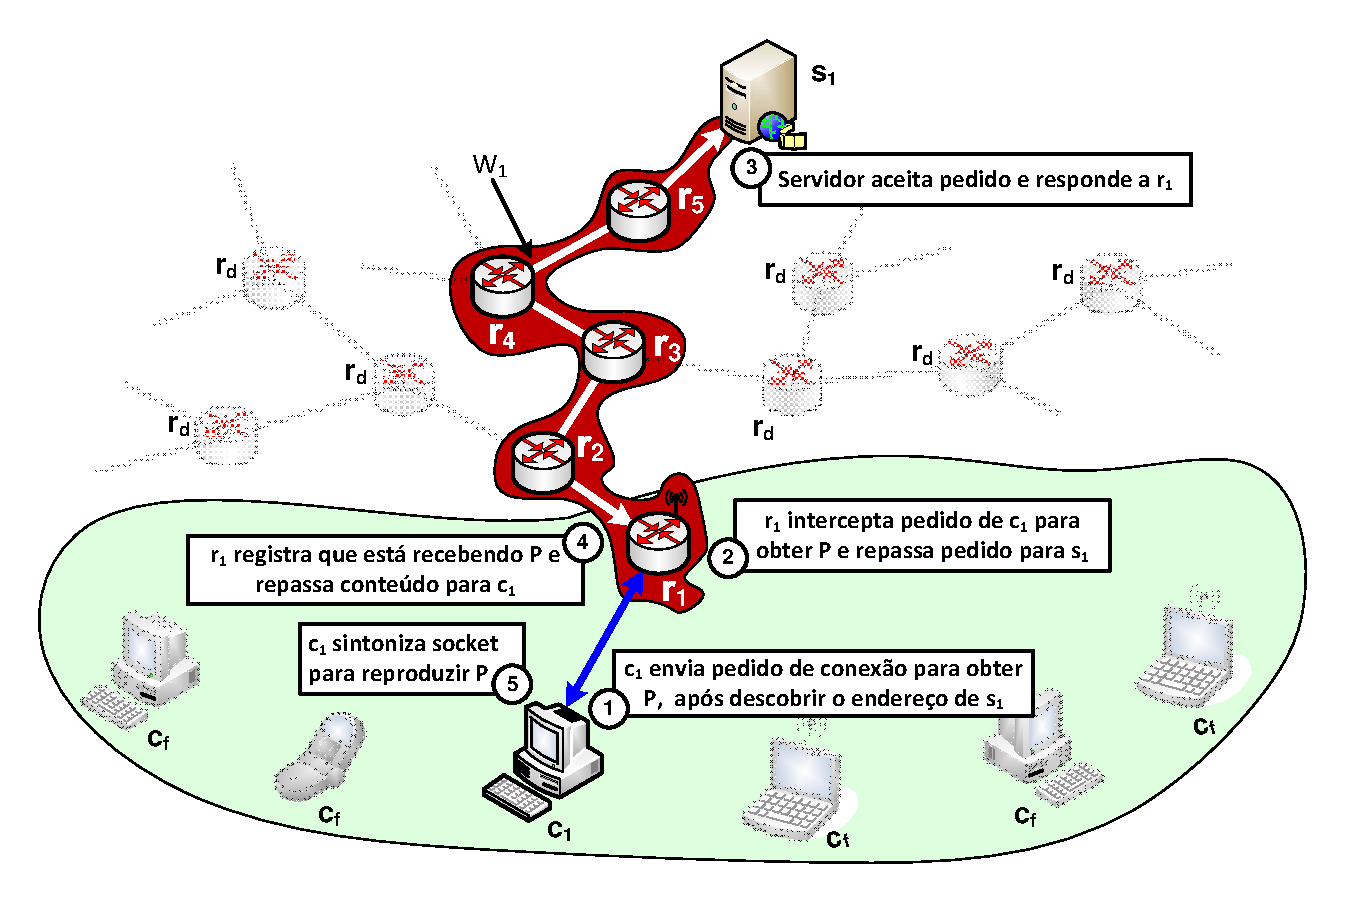
\includegraphics[scale=.7]{imgs/processo-conexao-1.pdf}
\end{center}
\vspace{-1cm}
\caption{Passos do processo de estabelecimento de conex�o do \mudccps (Fase 1).}
\label{fig:processo-conexao-1}
\end{figure}

\begin{itemize}

  \item \setpk, um fluxo de dados;

  \item \servu{1}, o servidor que gera os pacotes de dados \pks $\in$ \setpk;

  \item \repassu{1}, o repassador dos n�s \clis $\in$ \subsetcli$($\repassu{1}$)$; e

  \item \cliu{1}, um cliente que deseja obter um fluxo de dados \setpk, tal que \cliu{1} $\in$ \subsetcli$($\repassu{1}$)$.

\end{itemize}

Como ilustra-se na Figura~\ref{fig:processo-conexao-1}, para obter o fluxo de dados \setpk, o n� \cliu{1} inicia o canal de controle GMTP (detalhado na Se��o~\ref{subsec:canaiscommudccp}) e transmite um pacote do
tipo \pac{GMTP-Request} (Passo 1 da Figura~\ref{fig:processo-conexao-1}). Para construir o pacote do tipo \pac{GMTP-Request}, qualquer n� \clis deve especificar o valor para o endere�o IP de destino como sendo o endere�o do n� \servs que transmite \setpk, com o valor para o campo do cabe�alho de rede \textit{TTL=1}. Al�m dos valores para o IP de destino e para o \textit{TTL}, o n� \clis tamb�m deve informar o nome do fluxo de dados \setpks que o usu�rio deseja reproduzir, presente no cabe�alho de transporte do pacote do tipo \pac{GMTP-Request}. O valor de \textit{TTL=1} � intencional, pois faz com que o n� \repasss intercepte o referido pacote de requisi��o, evitando-se extrapolar o dom�nio administrativo de sua rede local. Este n�vel de detalhe � essencial para garantir que o roteador gerar� uma interrup��o atrav�s do processo que controla a fila de roteamento quando o \textit{TTL=0}, obrigando o roteador analisar o pacote e nesse momento perceber� que � um pacote do tipo \pac{GMTP-Request}. Isso evita que o roteador tenha que verificar se todos os pacotes correspondem ao tipo \pac{GMTP-Request}, reduzindo-se a carga de processamento e portanto o atraso nodal.

Quando o pacote \pac{GMTP-Request} alcan�ar o n� \repassu{1} (Passo 2), este consulta a tabela de recep��o de fluxos de dados e constata que n�o h� qualquer registro para o fluxo de dados \setpk. Nesse instante, o n� \repasss inicia um processo de registro de participa��o para obter o fluxo de dados \setpk. Isto significa que a execu��o do procedimento \textit{registerRelay(\serv, \pk)}, onde \pks � o pacote do tipo \pac{GMTP-Request}, far� o n� \repassu{1} transmitir um pacote do tipo \pac{GMTP-Register} em dire��o ao n� \servu{1}, conforme discutiu-se na Se��o~\ref{subsec:registro-participacao}. � medida que os n�s \repasss repassam o pacote \pac{GMTP-Register} at� alcan�ar o n� \servu{1}, constitui-se o caminho \setwayiu{1} $=$ $\{$\repassu{1},\repassu{2},\repassu{3},\repassu{4},\repassu{5},\servu{1}$\}$ (Passo 3, destacado na cor vermelha), conforme discutiu-se na Se��o~\ref{sec:descparc}.

Em seguida, ao receber o pacote do tipo \pac{GMTP-Register-Reply}, como resposta ao registro de participa��o, o n� \repassu{1} cria um canal \textit{multicast} e envia um pacote do tipo \pac{GMTP-RequestNotify} para um ou mais n�s \clis $\in$ \subsetcli$($\repassu{1}$)$ (Passo 4). Esta notifica��o permitir� aos n�s \cli, aguardando para obter \setpk, ``sintonizarem'' seus respectivos \textit{sockets} no canal \textit{multicast} correspondente. No caso do exemplo supracitado, o n� \cliu{1}, ap�s sintonizar o \textit{socket} no canal \textit{multicast} informado pelo n� \repassu{1}, come�a a receber os pacotes de dados \pks do tipo \pac{GMTP-Data} ou \pac{GTMP-DataAck} (Passo 5).

No Algoritmo~\ref{algo:respondToClients}, resumem-se os passos descritos anteriormente para iniciar a transmiss�o dos pacotes de dados \pks $\in$ \setpks aos n�s \clis $\in$ \subsetcli$($\repass$)$, ap�s \repasss receber o pacote do tipo \pac{GMTP-RequestReply}. Nota-se que, o n� \repasss invoca tal procedimento nas Linhas~\ref{algo-line:respondToClients1} e~\ref{algo-line:respondToClients2} do Algoritmo~\ref{algo:registerRelay} e nas Linhas~\ref{algo-line:respondToClients3} e~\ref{algo-line:respondToClients4} do Algoritmo~\ref{algo:onReceiveGMTPRegisterReply} (Se��o~\ref{subsec:registro-participacao}). Como resultado da Fase 1, gera-se uma nova entrada na tabela de recep��o de fluxos de dados do n� \repass, tal como ilustra-se na Figura~\ref{fig:tabela-recepcao-fluxo-11}. Com base no exemplo citado, a tabela de recep��o antes vazia, agora cont�m uma entrada que informa a ocorr�ncia de recep��o do fluxo de dados \setpks $=$ \textit{72c44591-7d82-427c-825f-722f015787c1}, originado em \serv, cujo endere�o � \textit{177.135.177.241}, com porta de recep��o \textit{49170}. Al�m disso, define-se o canal \textit{multicast} no endere�o \textit{239.192.68.79} e porta \textit{1900}, atrav�s do qual os n�s \clis $\in$ \subsetcli$($\repass$)$ podem receber os pacotes de dados \pks $\in$ \setpk.

\begin{figure}[ht]
\begin{center}
\includegraphics[scale=.55]{imgs/tabela-recepcao-fluxo-11.pdf}
\end{center}
\vspace{-1cm}
\caption{Tabela de recep��o de fluxos de dados ap�s a Fase 1.}
\label{fig:tabela-recepcao-fluxo-11}
\end{figure}

\vspace{0.8cm}

\begin{algorithm}[H]
\label{algo:respondToClients}
\caption{respondToClients(\pk: \pac{GMTP-RequestNotify})}
\SetAlgoLined
\tcc{A \repasss node executes this Algorithm to respond to clients waiting for
receiving a flow \setpk. This algorithm is invoked in Lines~\ref{algo-line:respondToClients1}
and~\ref{algo-line:respondToClients2} of
Algorithm~\ref{algo:registerRelay} and in
Lines~\ref{algo-line:respondToClients3} and~\ref{algo-line:respondToClients4}
of the Algorithm~\ref{algo:onReceiveGMTPRegisterReply}.}

\SetKwFunction{Union}{Union}\SetKwFunction{getClientsWaitingForFlow}{getClientsWaitingForFlow}
\SetKwFunction{Union}{Union}\SetKwFunction{getCtrlChannel}{getCtrlChannel}
\SetKwFunction{Union}{Union}\SetKwFunction{getMediaDescription}{getMediaDescription}
\SetKwFunction{Union}{Union}\SetKwFunction{setPacketFieldValue}{setPacketFieldValue}
\SetKwFunction{Union}{Union}\SetKwFunction{getPacketFieldValue}{getPacketFieldValue}
\SetKwFunction{Union}{Union}\SetKwFunction{sendPktRdt}{sendPktRdt}
\SetKwFunction{Union}{Union}\SetKwFunction{sendPkt}{sendPkt}
\SetKwFunction{Union}{Union}\SetKwFunction{waitAck}{waitAck}
\SetKwFunction{Union}{Union}\SetKwFunction{startRelay}{startRelay}
\SetKwFunction{Union}{Union}\SetKwFunction{removeClientsWaitingForFlow}{removeClientsWaitingForFlow}

% \clis \attrib \getPacketFieldValue{\pk, `client'}\;
\textit{destAddress} \attrib \getCtrlChannel{}\tcc*[r]{238.255.255.250:1900}
\setPacketFieldValue{\pk, `destinationAddress', destAddress}\;
\textit{\setpk} \attrib \getPacketFieldValue{\pk, `flow'}\tcc*[r]{Extracts \setpks in \pk}

\textit{errorCode} \attrib \getPacketFieldValue{\pk, `errorCode'}\;
\If(){errorCode $\neq$ NULL} {
  \removeClientsWaitingForFlow{\setpk}\tcc*[r]{See Algorithm~\ref{algo:registerRelay}}
  \sendPkt{\pk}\;
  \Return{0}\;
}

\textit{channel} \attrib \getPacketFieldValue{\pk, `channel'}\;
\label{algo-line:respondToClients-getChannel}
\uIf () {\textit{channel} $\neq$ NULL} {
  \tcc{Node \repasss is already receiving \setpks and clients \subsetcli$($\repass$)$ must know the media description.}
  \textit{mediaDescription} \attrib \getMediaDescription{\setpk}\;
  \setPacketFieldValue{\pk, `data', mediaDescription}\;
  \tcc{In Algorithm~\ref{algo:registerRelay}, Line~\ref{algo-line:addClientWaitingFlow}, \clis nodes are added in a list of clients waiting for flow \setpk. Now, \repasss notifies them, wait confirmation (ACKs) from them and start relaying \pks $\in$ \setpks to them through given channel.}
  \sendPkt{\pk}\;
  \subsetcli$($\repass$)$ \attrib \getClientsWaitingForFlow{\setpk}\;
  \waitAck{\subsetcli$($\repass$)$, \setpk}\;
  \label{algo-line:respondToClients-waitAck}
} \Else (\tcc*[f]{Let \subsetcli$($\repass$)$ know \repasss is waiting for registration.}) {
  \setPacketFieldValue{\pk, `waitingRegistration', true}\;
  \sendPkt{\pk}\;
}
\Return{0}\;

\end{algorithm}
\vspace{0.8cm}

\subsection{Fase 2: pr�ximas requisi��es para obter \setpk}

A Fase $2$ de conex�o ocorre quando futuras requisi��es para obter o fluxo de dados \setpks s�o originadas por qualquer n� \clis $\in$ \subsetcli$($\repassu{1}$)$. Considerando o exemplo anterior, citado na Fase 1,
se um n� \cliu{2} $\in$ \subsetcli$($\repassu{1}$)$ tamb�m solicitar \setpk, o n� \repassu{1} simplesmente informar� o canal \textit{multicast} correspondente ao fluxo de dados \setpk, como ilustra-se na Figura~\ref{fig:processo-conexao-2} (Passo 1). Para isto, o n� \repassu{1} intercepta a requisi��o do n� \cliu{2}, consulta a tabela de recep��o de fluxos de dados e dessa vez constata a recep��o do fluxo de dados \setpk, criando o pacote do tipo \pac{GMTP-Request-Reply} (Passo 2). Este procedimento ocorre no registro de participa��o, especificamente no trecho de c�digo definidos entre as
Linhas~\ref{algo-line:registerRelay-getP}-\ref{algo-line:registerRelay-returnChannel} do Algoritmo~\ref{algo:registerRelay}. Em seguida, transmite-se o pacote do tipo \pac{GMTP-Request-Reply} ao n� \cliu{2}, como descreve-se no trecho de c�digo entre as
Linhas~\ref{algo-line:respondToClients-getChannel}-\ref{algo-line:respondToClients-waitAck} do Algoritmo~\ref{algo:respondToClients}, que ent�o ``sintoniza'' seu \textit{socket} para o canal \textit{multicast} informado por \repassu{1} (Passo 3). Tal procedimento se repete para cada novo n� \clis $\in$ \subsetcli$($\repassu{1}$)$ interessado em obter \setpk.

\begin{figure}[ht]
\begin{center}
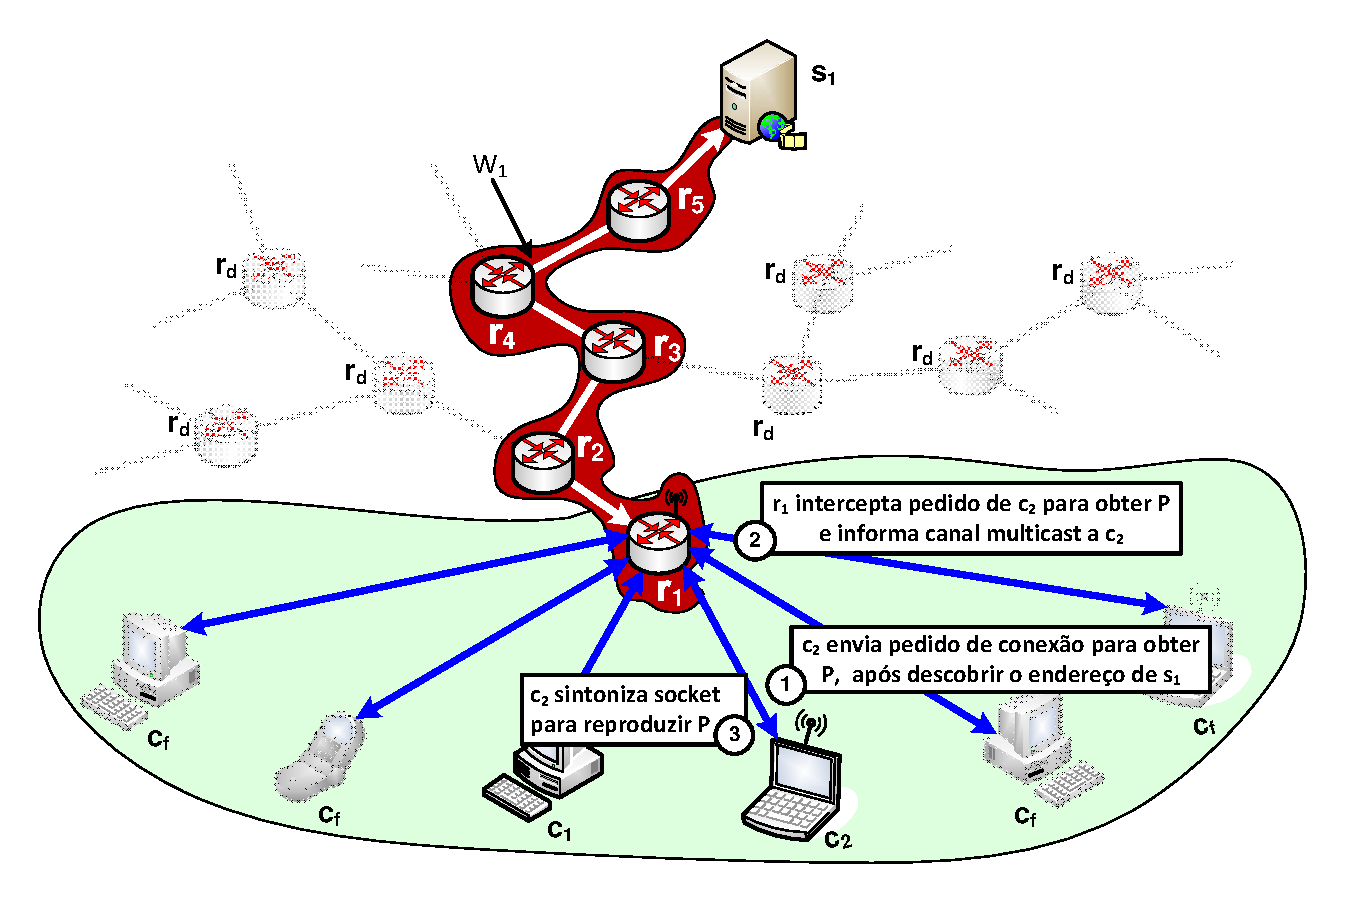
\includegraphics[scale=.6]{imgs/processo-conexao-2.pdf}
\end{center}
\vspace{-1cm}
\caption{Passos do processo de estabelecimento de conex�o do \mudccps (Fase 2).}
\label{fig:processo-conexao-2}
\end{figure}

\subsection{Fase 3: busca por mais parceiros \repassu{q} para obter \setpk}
\label{subsec:phase3}


% /////////////////////////////////
%
%
% \subsection{Sobre o melhor caminho \setwayi}
% \label{subsec:melhorcaminho}
%
% LER ISSO DAKI E O QUE EST� SENDO DESCRITO NESSA FASE 3. PENSAR NA ID�IA DE QUANDO
% O NO REPASS PROCURAR POR MAIS PARCEIROS, USAR
% O CRIT�RIO COM CAMINHOS MAIS FOLGADOS (MAIORES TAXAS DE TRANSMISS�O)
% %
% % \begin{algorithm}[H]
% % \label{algo:findPartnerIntersectPath}
% % \SetAlgoLined
% % \caption{handleRegisterParticipation(\repass: PeerRelay, \pks $=$
% % \pac{GMTP-Register})}
% % \tcc{\servs executes this algorithm to handle the request for register of
% % participation. It finds the first node \ways common to a known path \setwayis
% % and the path \setwayiu{\repassconst_\repassi}. \setwayis is already used for
% % transporting \setpks to node in $\delta($\way, \setwayi$)$, and
% % \setwayiu{\repassconst_\repassi} is the path composed by all nodes in between
% % \repasss and \serv. The packet \pks carries \setwayiu{\repassconst_\repassi} and
% % the \setpks name.}
% %
% % \SetKwFunction{Union}{Union}\SetKwFunction{makePkt}{makePkt}
% % \SetKwFunction{Union}{Union}\SetKwFunction{getPacketFieldValue}{getPacketFieldValue}
% % \SetKwFunction{Union}{Union}\SetKwFunction{recvPktRdt}{recvPktRdt}
% % \SetKwFunction{Union}{Union}\SetKwFunction{sendPktRdt}{sendPktRdt}
% % \SetKwFunction{Union}{Union}\SetKwFunction{length}{length}
% % \SetKwFunction{Union}{Union}\SetKwFunction{pathsContainingRelayByFlow}{pathsContainingRelayByFlow}
% % \SetKwFunction{Union}{Union}\SetKwFunction{GMTPRegisterReply}{GMTPRegisterReply}
% % \SetKwFunction{Union}{Union}\SetKwFunction{pathPriority}{pathPriority}
% %
% % \textit{\setpk} \attrib \getPacketFieldValue{\pk, `flow'}\tcc*[r]{Extracts \setpks in \pk}
% % \textit{\setwayiu{\repassconst_\repassi}} \attrib \invert{\getPacketFieldValue{\pk, `path'}}\;
% % \textit{\setwayiu{\setpkc}} \attrib \pathsContainingRelayByFlow{\repass, \setpk}\tcc*[r]{\setwayiu{\setpkc} $\subset$ \setway}
% % % \tcc*[r]{For a given flow and all the known paths \setways in this \serv, get a sub set of paths used to transmit \setpk}
% %
% % \setwayiu{selected} \attrib \setwayiu{\repassconst_\repassi}\;
% %
% % \ForEach{\setwayis $\in$ \setwayiu{\setpkc}}{
% %     \If() {\pathPriority{\setwayis > \setwayiu{selected}}} {
% %       \setwayiu{selected} \attrib \setwayi\;
% %     }
% % }
% %
% % \ForEach{\ways $\in$ \setwayiu{selected}} {
% %   \If(){\ways $\in$ \textit{\setwayiu{\repassconst_\repassi}}} {
% %     \tcc{The node \ways is common in \setwayis and in \textit{\setwayiu{\repassconst_\repassi}}.}
% %     \textit{done} \attrib \textit{true}\;
% %     break\;
% %   }
% % }
% %
% %     \If(){\textit{done}} {
% % %       \tcc{Create a \pac{GMTP-Response} and send it to \way. After receiving \textit{\pk}, \ways becomes a relay of the flow \setpk.}
% % %       \pks \attrib \makePkt{\pac{GMTP-Response}(1), \ways}\;
% %       \tcc{\servs stores \textit{\setwayiu{\repassconst_\repassi}} as a known path and replies to \repass, asking \ways to act as a relay for \setpk. \servs actives flag 'relay' of the \pac{GMTP-RegisterReply}.}
% %       \setwayiu{\setpkc}[\length{\setwayiu{\setpkc}}] \attrib \textit{\setwayiu{\repassconst_\repassi}}\;
% %       \Return{\GMTPRegisterReply{\way, relay=1}}\;
% % %       \sendPktRdt(\pk)\;
% % %       \exit{}\;
% %     }
% %
% % \tcc{\servs must register \textit{\setwayiu{\repassconst_\repassi}} as a known path and reply to \repasss by accepting its connection request, since no node \ways is intersecting \textit{\setwayiu{\repassconst_\repassi}}. In this case, \servs starts the transmission of \pks $\in$ \setpks to \repass.}
% % \setway[\length{\setway}] \attrib \textit{\setwayiu{\repassconst_\repassi}}\;
% % \Return{\GMTPRegisterReply{\repass, relay=0}}\;
% % % \pks \attrib \makePkt{\pac{GMTP-Response}(0), \repass}\;
% % % \sendPktRdt(\pk)\;
% %
% % \end{algorithm}
% % \vspace{0.8cm}
%
% De acordo com os procedimentos empregados de sele��o de n�s, � poss�vel obter
% diferentes caminhos \setwayi, partindo-se de um n� \repasss para um n� \serv.
% Por este motivo, � importante definir, a partir de um conjunto de caminhos
% poss�veis, qual � o melhor caminho a utilizar e orden�-los de acordo com a
% prioridade de uso. Com isto, � poss�vel obter \setpks a partir de m�ltiplos
% \repasss e usar caminhos alternativos em caso de falha de algum caminho, por
% exemplo, por desconex�o. No GMTP, utiliza-se os seguintes crit�rios para
% decidir entre um conjunto de caminhos \setway qual ser� o escolhido:
%
% \begin{enumerate}
%   \item Quanto mais o caminho \setwayis estiver pr�ximo de ser um caminho
% \setwayif; \label{i:c-waycomp}
%   \item Menor n�mero de n�s \ways $\in$ \setwayi; \label{i:c-nnos}
%   \item Escolha aleat�ria de \setwayis entre os \setways conhecidos.
% \label{i:c-aleat}
% \end{enumerate}
%
% O crit�rio~\ref{i:c-waycomp} � determinado atrav�s da verifica��o da condi��o
% $\mid$\setwayi$\mid$ $=$ $ttl($\repass$,$\setwayi$)$, onde \textit{ttl} � uma
% fun��o que determina o n�mero de saltos entre o n� \repasss at� o n� \serv. Na
% pr�tica, pode-se determinar tal condi��o comparando-se quantos n�s existem no
% caminho \setwayis e o valor do campo TTL (\textit{Time-to-Live}), dispon�vel no
% cabe�alho de qualquer pacote IP. Este crit�rio � o prim�rio porque quanto mais
% n�s GMTP estiverem no caminho, maior ser� a possibilidade de intercepta��o
% para obter um fluxo de dados \setpk. O crit�rio~\ref{i:c-nnos} � determinado
% pela contagem do n�mero de \ways $\in$ \setwayi. O crit�rio~\ref{i:c-aleat} �
% utilizado em caso de n�o determina��o do melhor \setwayis at� o crit�rio
% anterior.
%
% Note que no GMTP � poss�vel que um n� \repasss tenha simultaneamente mais de um
% n� parceiro \repassu{q}, por�m n�o mais do que uma certa qualidade configur�vel
% devido ao fato de que os pacotes \pks dos fluxos \setpks serem transientes,
% portanto n�o faz sentido realizar muitas parcerias. No caso do GMTP, a
% quantidade m�xima padr�o de parcerias que um n�s \repasss realiza � $5$, valor
% praticado em outros solu��es similares para transmiss�o de fluxos de dados ao
% vivo baseados em arquitetura P2P.
%
%
%
% /////////////////////////////////


Na Fase $3$, o n� \repasss inicia um processo de aumentar suas parcerias a fim
de obter mais rapidamente os pacotes \pks $\in$ \setpk, atrav�s de caminhos
\setwayis alternativos.
% , em caso de falha e/ou desconex�es de algum n� parceiro
% \repassu{q}.
% Ao
% considerar os aspectos discutido na Se��o~\ref{sec:descparc}, nota-se que na
% Fase $1$ e $2$ utiliza-se os modos de forma��o de parcerias intra \setways e por
% intersec��o, por�m ainda resta fazer uso do modo de forma��o de parceria por
% combina��o de \setway
% (Figura~\ref{fig:esquema-abstrato-formacao-parceria-combinacao}). Na fase $3$ de
% conex�o, o GMTP explora tal recurso.
Para isto, o n� \servs constr�i uma lista de n�s parceiros e envia ao n� \repass, funcionando como um indexador de n�s parceiros \repassu{q}, pr�-selecionando parceiros para \repass. Por exemplo, seja um n� \repassu{3} que esteja recebendo \setpks originado em um n� \serv, como ilustra-se na Figura~\ref{fig:conn-phase3-1}. Para conseguir mais n�s parceiros \repassu{q}, o n� \repassu{3} envia uma requisi��o do tipo \pac{GMTP-RelayQuery} para \servs e obt�m um subconjunto de n�s \repassu{q} candidatos a parceiro de \repassu{3}. No caso do exemplo supracitado, essa pr�-sele��o ajuda o n� \repassu{3} a escolher os melhores parceiros dispon�veis, de acordo com os seguintes crit�rios de prioridade:

\begin{figure}[b!ht]
\begin{center}
\includegraphics[scale=0.9]{imgs/gmtp-conn-phase3-1.pdf}
\end{center}
\vspace{-1cm}
\caption{Fase 3 de conex�o do GMTP (Passo 1).}
\label{fig:conn-phase3-1}
\end{figure}

\begin{enumerate}

  \item Maior capacidade de transmiss�o do caminho \setwayi. Define-se este crit�rio com base na menor taxa de transmiss�o dispon�vel entre todos os n�s \ways $\in$ \setwayis em um determinado instante \textit{t}. Na Se��o~\ref{sec:ccgmtp}, discutem-se os algoritmos de controle de congestionamento do GMTP e o procedimento para determinar a taxa de transmiss�o de um caminho \setwayi;
  \label{i:c-maiortranstx}

  \item Se for um caminho for \setwayif, determinado atrav�s da verifica��o da
condi��o $\mid$\setwayi$\mid$ $=$ $ttl($\repass$,$\setwayi$)$, onde \textit{ttl}
� uma fun��o que determina o n�mero de saltos entre o n� \repasss at� o n�
\serv. Este crit�rio � importante porque quanto mais n�s GMTP estiverem no
caminho, maior ser� a possibilidade de intercepta��o para obter um fluxo de
dados \setpk;
  \label{i:c-waycomp}
%
%   \item Menor n�mero de n�s \ways $\in$ \setwayi;
%   \label{i:c-nnos}

  \item Escolha aleat�ria de \setwayis entre os caminhos \setways conhecidos. Nota-se que, por exemplo, no CoolStreaming, a escolha aleat�ria � feita em n�vel de cliente, ao passo que no GMTP a escolha � com base na capacidade de transmiss�o dos caminhos \setwayis $\in$ \setway.
  \label{i:c-aleat}

\end{enumerate}

Sendo assim, define-se a Fase $3$ do processo de estabelecimento de conex�o do
GMTP em tr�s passos:

\begin{enumerate}

  \item Um n� \repasss envia periodicamente requisi��es do tipo \pac{GMTP-RelayQuery} para o n� \servs a fim de descobrir melhores parceiros e aumentar o n�mero de parcerias. Por se tratar de fluxos de dados ao vivo, n�o necessariamente quanto mais parceiros um n� \repasss tem, melhor ser� a qualidade do fluxo de dados \setpk. Por isso, um n� \repasss sempre mant�m uma lista de candidatos a parceiros \repassu{q} fornecida pelo n� \serv, por�m n�o necessariamente estabelece parcerias com todos. Em vez disso, executam-se, repetidamente, as seguintes a��es:

\begin{itemize}

  \item Um n� \repasss inicia uma nova parceria se a quantidade atual de
parcerias reduzir por desconex�o de um n� parceiro \repassu{q} ou se o \textit{buffer} de
recep��o estiver com menos de $\frac{1}{3}$ de sua capacidade. O objetivo �
evitar o esvazeamento do \textit{buffer} para o fluxo de dados \setpk, mantendo
continuamente o repasse de pacotes de dados \pks $\in$ \setpks aos n�s \clis
$\in$ \subsetcli$($\repass$)$.

  \item A quantidade de parcerias em um determinado instante \textit{t} �
inversamente proporcional a quantidade de pacotes de dados \pks $\in$ \setpks
que chegam repetidos ao n� \repass. Nesse caso, se um mesmo pacote \pks chegar
repetidamente na mesma quantidade de parcerias estabelecidas, o n� \repasss
desconecta-se daquele n� parceiro \repassu{q} cujo pacote \pks chegou por �ltimo.

\end{itemize}

  \item Ap�s obter a lista de candidatos a parceiros (Passo 1), o n� \repassu{3} forma uma parceria com um dos candidatos da lista de poss�veis parceiros. Para isto, o n� \repassu{3} envia requisi��es do tipo \pac{GMTP-Request} em dire��o a outros n�s \repassu{q} sugeridos por \servs e que j� estejam recebendo um fluxo de dados \setpk. Como ilustra-se na Figura~\ref{fig:conn-phase3-2}, este procedimento ocorre da seguinte forma: o n� \repassu{3} envia uma requisi��o do tipo \pac{GMTP-Request} para o n� \repassu{2}, contendo uma chave de autoriza��o conhecida por ambos e informada pelo n� \serv. Caso a chave de autoriza��o esteja correta, o n� \repassu{2} deve enviar um resposta do tipo \pac{GMTP-Response} ao n� \repassu{3} e ent�o come�ar a repassar os pacotes \pks $\in$ \setpk. O uso da chave de autoriza��o � importante para evitar que um n� \repasss se conecte a outro n� \repassu{q} sem que o n� \servs seja notificado sobre isto. As chaves de autoriza��o s�o geradas pelo n� \servs e transmitidas como resposta no pacote do tipo \pac{GMTP-Register-Reply}. Cada entrada dispon�vel no pacote do tipo \pac{GMTP-RelayQuery-Reply} cont�m o identificador do repassador candidado a parceiro e sua respectiva chave de autoriza��o.

\end{enumerate}

\begin{figure}[ht]
\begin{center}
\includegraphics[scale=0.9]{imgs/gmtp-conn-phase3-2.pdf}
\end{center}
\vspace{-1cm}
\caption{Fase 3 de conex�o do GMTP (Passo 2).}
\label{fig:conn-phase3-2}
\end{figure}


% Como se considera uma arquitetura h�brida P2P/CDN, o n� \servs pode realizar uma
% fun��o de balanceamento de carga, incluindo como resposta de uma requisi��o do
% tipo \pac{GMTP-RelayQuery} os outros n�s \serv, levando-se em considera��o,
% inclusive, todos os crit�rios estabelecidos na
% Se��o~\ref{subsec:melhorcaminho}.

A periodicidade de requisi��es do tipo \pac{GMTP-RelayQuery} e a quantidade m�xima de parcerias efetivas s�o par�metros control�veis pelo administrador do n� \repass. Na implementa��o do GMTP utilizada neste trabalho, definiu-se o tempo de 5 minutos para a periodicidade de requisi��es do tipo \pac{GMTP-RelayQuery} e 5 para a quantidade de parcerias efetivas.

Com a execu��o da Fase 3 do processo de conex�o do GMTP, pode-se expandir a quantidade de parcerias, registradas na tabela de recep��o de fluxos de dados, tal como ilustra-se na Figura~\ref{fig:tabela-recepcao-fluxo}. Nesse exemplo, observa-se que um n� \repasss est� recebendo e repassando aos seus n�s \clis $\in$ \subsetcli$($\repass$)$ quatro fluxos de dados diferentes, originados em quatro n�s \serv, por�m recebendo fluxos de dados de diferentes n�s parceiros \repassu{q}. Por exemplo, dentre os fluxos de dados que o n� \repasss est� recebendo, um deles � o \setpks $=$ \textit{72c44591-7d82-427c-825f-722f015787c1}, cujos pacotes de dados \pks $\in$ \setpks s�o transmitidos por tr�s n�s \repassu{q} identificados pelos
endere�os IP e porta \textit{182.111.88.21:49170}, \textit{90.39.135.46:62242} e \textit{83.67.132.41:53434}. Para esse fluxo de dados \setpk, o n� \repasss repassa os pacotes de dados \pks para os n�s \clis $\in$ \subsetcli$($\repass$)$ atrav�s do canal \textit{multicast} \textit{239.192.68.79:1900}.

\begin{figure}[htb!]
\begin{center}
\includegraphics[scale=.55]{imgs/tabela-recepcao-fluxo.pdf}
\end{center}
\vspace{-1cm}
\caption{Tabela de recep��o de fluxos de dados ap�s a Fase 3.}
\label{fig:tabela-recepcao-fluxo}
\end{figure}

% \subsection{Compartilhamento de \setpks entre \servs}
% \label{subsec:compartilhamento-de-p}
%
% Al�m do procedimento transparente � aplica��o para se obter um fluxo de dados
% \setpk, como os n�s \servs constituem uma rede CDN, estes podem negociar entre
% si o envio e a recep��o de um fluxo de dados \setpks de acordo com as
% requisi��es submetidas aos n�s \repass. Desta forma, se um n� \repasss enviar
% uma requisi��o para obter \setpks de um evento \events a um n� \servs e este n�o
% esteja recebendo tal fluxo, \servs poder� solicit�-lo a outros n�s \servs da
% CDN que participa. A partir desse ponto, o n� \servs passar� a servir o n�
% \repasss normalmente. Como no GMTP se faz uso indireto dessa fun��o das redes
% CDNs, a qual j� est� consolidada, resolveu-se suprimir maiores detalhes a
% respeito deste assunto. Para maiores informa��es sobre a fun��o de distribui��o
% de conte�dos ao vivo entre os servidores de uma rede CDN, o leitor pode
% consultar as
% refer�ncias~\cite{Nygren:2010:ANP:1842733.1842736,1250586,Pathan2008}.
%
\vspace{0.5cm}

Desta forma, o processo de conex�o do GMTP � fundamental para a efetiva distribui��o de m�dias ao vivo, pois permite que as aplica��es compartilhem fluxos de dados entre si, mesmo que estas n�o tenham sido desenvolvidas pelo mesmo fornecedor. Esta unifica��o ajuda no processo de distribui��o do fluxo de dados \setpk, pois at� mesmo uma aplica��o \textit{standalone} e um objeto de v�deo imbutido em uma p�gina Web podem obter o mesmo fluxo de dados sem que estas conhe�am uma a outra. Consequentemente, reduz-se para 1 o n�mero de transmiss�es para um mesmo fluxo de dados \setpks originado em \servs e destinados a uma mesma rede ou para um subconjuntos de redes adjacentes. Al�m dessa diferen�a, a forma de conex�o do GMTP supre uma antiga defici�ncia das solu��es tradicionais de transmiss�o \textit{multicast}, pois as aplica��es tinham que se adaptar �s configura��es est�ticas dos canais \textit{multicast}, definidos pelo administrador de rede, e os pr�prios administradores de rede tinham que fazer tal configura��o de forma manual, obrigatoriamente em todos os n�s roteadores de um determinado caminho. Isto � impratic�vel devido � independ�ncia dos diferentes dom�nios administrativos.

Desta forma, n�o se tem conhecimento de uma solu��o que permita configura��o din�mica de canais \textit{multicast} aliada � forma��o de uma rede de favores constitu�da entre roteadores. Constitui-se a rede de favores atrav�s da forma��o de parcerias pela intersec��o de rotas que se tornam conhecidas � medida que novos clientes se interessam por uma mesma m�dia, sendo este processo regido por um servidor \textit{pivot} transmissor da m�dia, que sugere as parcerias com base na capacidade de transmiss�o dos canais em uso. Nesse contexto, compartilham-se os fluxos de dados entre aplica��es de diferentes fornecedores, resultando no uso mais eficiente dos recursos computacionais e de rede. Os resultados obtidos com o uso dessa estrat�gia ser�o discutidos mais adiante no Cap�tulo~\ref{cap:analisedesemp}.

\subsection{Envio e recebimento de \pks $\in$ \setpks em \net}
\label{subsec:trocdados}

Ap�s o estabelecimento de conex�o, os n�s \repasss trocam dados entre si em modo
\textit{unicast} a fim de distribuir os pacotes de dados \pks $\in$ \setpks do tipo
\pac{GMTP-Data} e \pac{GMTP-DataAck}. De forma similar, os n�s \repasss
utilizam os mesmos tipos de pacotes para enviar \pks $\in$ \setpks para os n�s
\cli, por�m em modo \textit{multicast}. Quando o \mudccps estiver em funcionamento em
um n� \servs ou em um \repass, o estado � o de \textit{transmitindo dados}, ao
passo que quando executado em um cliente o estado � o de \textit{recep��o de
dados}. Para o transporte dos pacotes de dados \pk, um n� \servs deve transmitir
pacotes do tipo \pac{GMTP-Data} ou o \pac{GMTP-DataAck} em dire��o aos n�s
\repasss de acordo com os registros de partipa��o. Nesta se��o, detalha-se como
se executa os procedimentos de transmiss�o e recep��o desses pacotes de
dados.

% Embora o
% protocolo \mudccps transmite dados sem garantia de entrega, a aplica��o pode
% determinar que certos dados sejam transmitidos com garantia de entrega. Nestes
% casos, durante a transmiss�o de dados, um n� \mudccps utiliza-se do pacote do
% tipo \pac{GMTP-Data} para enviar dados, ao passo que utiliza-se pacote
% \pac{GMTP-Ack} para confirmar a recep��o de pacotes, ou ainda, utiliza-se
% \pac{GMTP-DataAck} para enviar pacotes de dados e ao mesmo tempo confirmar a
% recep��o de pacotes de dados vindos da dire��o oposta (\textit{piggyback}).

\subsubsection{\textit{Buffer} de envio e recep��o:}

A transmiss�o de um evento \events consiste no processo de dissemina��o
dos pacotes \pks $\in$ \setpks atrav�s dos n�s interessados em obt�-lo. Para
isto, cada n� GMTP controla um \textit{buffer} de envio e recep��o definido por uma
estrutura de dados do tipo \textit{array} circular (\textit{ring buffer}), onde cada
posi��o � utilizada para armazenar um pacote \pk, como ilustra-se na
Figura~\ref{fig:buffer-envio-recepcao-ring}. Ao receber \pk, um n� GMTP
armazena-o no \textit{buffer} e posteriormente o entrega para a aplica��o, que o
reproduz para o usu�rio final. Para o envio ou repasse de um pacote, o n� GMTP
consome os pacotes \pks do \textit{buffer} e transmite para o(s) n�(s) interessado(s),
seja em modo \textit{unicast} e/ou em modo \textit{multicast}. Isto porque � poss�vel que um n�
\repassu{1} repasse \pks para um outro n� \repassu{2} (\textit{unicast}) ao mesmo tempo
que \repassu{1} pode repassar \setpks para seus n�s \clis (\textit{multicast}).

O \textit{buffer} de envio e recep��o do GMTP tem seu tamanho definido no processo de
estabelecimento de conex�o, de acordo com o tipo da m�dia sendo transmitido, mas o n� \repasss pode determinar um limite a fim de evitar ataques de nega��o de servi�o. Isto pode ocorrer porque o GMTP permite uma aplica��o definir o tamanho do \textit{buffer} que cada n� \ways dever� alocar para repassar os pacote de dados \pks de um fluxo de dados \setpk. Ent�o, uma aplica��o maliciosa poderia alocar um espa�o de \textit{buffer} maior do que a que o roteador suporta, ou no m�nimo monopolizar tal \textit{buffer}. Ap�s definir o tamanho inicial do \textit{buffer} circular para um fluxo de dados \setpk, este pode variar de acordo com a capacidade de transmiss�o do canal em um determinado instante. Essa decis�o � importante porque permite um n� \servs alocar previamente o recurso necess�rio para o transporte de um determinado fluxo de dados \setpk. O tamanho do \textit{buffer} � especificado pelo n�
\servs e propagado para os demais n�s em um caminho \setway, no cabe�alho do
pacote do tipo \pac{GMTP-Register-Reply} ou \pac{GMTP-MediaDesc}.

\begin{figure}[ht]
\begin{center}
\includegraphics[scale=1]{imgs/buffer-envio-recepcao-ring.pdf}
\end{center}
\vspace{-1cm}
\caption{Exemplo da estrutura do \textit{buffer} de envio e recep��o de um n� GMTP com
dois ponteiros, um para escrever e outro para ler pacotes \pk.}
\label{fig:buffer-envio-recepcao-ring}
\end{figure}

\subsubsection{Mapa de \textit{buffer}:}

O mapa de \textit{buffer} do GMTP descreve o estado atual do \textit{buffer} de envio e recep��o
de um n� GMTP. Como ilustrado na Figura~\ref{fig:mapa-buffer-envio-recepcao},
trata-se de uma estrutura de dados que determina se um pacote \pks est�
ou n�o presente no \textit{buffer} de um respectivo n� GMTP. O conte�do de cada posi��o
� o n�mero de sequ�ncia do pacote, que determina a ordem que um pacote foi
gerado e transmitido pelo n� \serv, mas o n� \repasss n�o os ordena, pois tal responsabilidade � delegada aos n�s \clis no momento de sua reprodu��o ao usu�rio final.

\begin{figure}[ht]
\begin{center}
\includegraphics[scale=0.76]{imgs/mapa-buffer-envio-recepcao.pdf}
\end{center}
\vspace{-1cm}
\caption{Exemplo do mapa de \textit{buffer} de um n� GMTP com tamanho de 17 \pk.}
\label{fig:mapa-buffer-envio-recepcao}
\end{figure}

Um n� GMTP utiliza o mapa de \textit{buffer} para sinalizar seu atual estado com rela��o a um determinado fluxo de dados \setpk. Um n� GMTP pode enviar o mapa de \textit{buffer} completo, como ilustrado na Figura~\ref{fig:mapa-buffer-envio-recepcao}, ou o mapa de \textit{buffer} apenas dos \pks presentes ou ausentes. Na pr�tica, quando deseja indicar a sua atual disponibilidade, um n� \repasss envia para um n� parceiro \repassu{q} o mapa de \textit{buffer} dos \pks presentes e, quando desejar obt�-los, envia o mapa de \textit{buffer} dos \pks ausentes. Para diferen�ar o tipo de requisi��o, utiliza-se uma sinaliza��o bin�ria (\textit{flag}) chamada \textit{request-type}, onde $0$ significa que o mapa de \textit{buffer} cont�m pacotes
dispon�veis e $1$, pacotes ausentes. Note que, quando um n� \repasss transmite
um mapa de \textit{buffer} para um outro n� qualquer \repassu{q}, caracteriza-se automaticamente o uso do m�todo \textit{pull}, em vez do m�todo \textit{push}, que � o modo padr�o do GMTP. Salienta-se ainda que deve-se evitar o m�todo pull devido � transitoriedade dos pacotes de dados \pks (transmiss�o de dados ao vivo) e um n� \repasss deve apenas realiza tal procedimento ap�s completar a Fase 3 do processo de estabelecimento de conex�o. Isto porque um n� \repasss pode nunca receber a resposta para uma requisi��o do tipo \textit{pull}. Essa sinaliza��o ocorre atrav�s do uso do pacote do tipo \pac{GMTP-DataPull-Request}, que � preenchido com o mapa de \textit{buffer} dos pacotes ausentes e transmitido aos respectivos n�s parceiros. Ao receber esse tipo de requisi��o, um n� parceiro avalia seu conte�do e responde com o pacote do tipo \pac{GMTP-DataPull-Response}, o qual cont�m o mapa de \textit{buffer} dos pacotes dispon�veis, seguido dos pacotes \pks do tipo \pac{GMTP-Data}. Note que os pacotes do tipo \pac{GMTP-DataPullRequest} e \pac{GMTP-DataPull-Response} s�o transmitidos com garantia de entrega.

% , ou seja, caso sejam perdidos, o GMTP
% garante sua retransmiss�o. Para isto, o GMTP utiliza o mecanismo b�sico de
% envio e confirma��o utilizando o pacote do tipo \pac{GMTP-DataAck} ou
% \pac{GMTP-DataAck}. No caso de falha na execu��o de uma requisi��o utilizando o
% m�todo \textit{pull}, o n� GMTP pode reavaliar a necessidade de retransmitir o
% pedido, pois � poss�vel que os \pks ausentes j� tenham expirados e requisit�-los
% novamente n�o far� mais sentido.

Na pr�tica, o mapa de \textit{buffer} utilizado para sinalizar a presen�a ou aus�ncia de
\pks � representado por faixas de acordo com o �ndice do \textit{buffer}. Por exemplo,
para representar o mapa de \textit{buffer} dos pacotes ausentes ilustrados na
Figura~\ref{fig:mapa-buffer-envio-recepcao}, o n� GMTP preenche o pacote do
tipo \pac{GMTP-DataPull-Request} com a sequencia \textit{2;6-10;12}. Ao receber
esta sequ�ncia, o n� parceiro \repassu{q} responde com o pacote do tipo
\pac{GMTP-DataPull-Response}, que cont�m o mapa de \textit{buffer} de quais
pacotes ser�o enviados e come�a a transmit�-los.

% * RELATAR TAXA DE RECEPCAO	- NO RELATA QUAL A TAXA DE RECEP��O
% (PREENCHIMENTO+ATUALIZA��O DO BUFFER)
% * USA ESSA INFO PARA SELECIONAR OS MELHORES PARCEIROS (FILTRO APRIMORADO)

\subsubsection{Descarte de pacotes:}

O descarte de pacotes \pks ocorre sempre no repassador e em duas situa��es:

\begin{enumerate}

 \item \textbf{Por transbordo do buffer:} o transbordo do \textit{buffer} pode ocorrer devido ao mecanismo de controle de congestionamento empregado no GMTP, que pode reduzir a taxa de transmiss�o enquanto novos pacotes precisam ser alocados no \textit{buffer}. Sendo assim, deve-se descartar os primeiros pacotes \pks recebidos se o \textit{buffer} alcan�ou seu limite, mesmo que ainda n�o tenham sido repassados. Uma otimiza��o n�o explorada neste trabalho, mas que � poss�vel de ser realizada, � o descarte seletivo de pacotes, primeiro os que tenham menos impacto na qualidade da m�dia, por exemplo, pacotes de dados contendo quadros B (codifica��o MPEG4, tipo 2). O descarte seletivo de pacotes n�o impede que o v�deo seja reproduzido, por�m com perda de qualidade, mas ao menos se permite a transmiss�o dos pacotes de dados \pks de acordo com a largura de banda dispon�vel;

 \item \textbf{Por duplica��o:} ocorre quando o pacote \pks j� foi recebido anteriormente. Tal verifica��o � feita de acordo com o n�mero de sequ�ncia presente em cada pacote \pk. Essa contagem � importante e pode determinar que um n� \repasss desconecte de um n� parceiro \repassu{q}, tal como explicou-se na Se��o~\ref{subsec:phase3}.

\end{enumerate}

\section{Controle de Congestionamento em \net}
\label{sec:ccgmtp}

No GMTP, executa-se um algoritmo para controle de congestionamento h�brido, cujo comportamento depender� do modo de transmiss�o sendo utilizado para transportar os pacotes de dados \pks $\in$ \setpks (\textit{unicast} ou em \textit{multicast}). Como ilustra-se na Figura~\ref{fig:ucc-mcc-esquema}, tratam-se de dois algoritmos para controle de congestionamento, um que atua em transmiss�es \textit{unicast}, chamado de \textit{\mudccps Unicast Congestion Control} (GMTP-UCC) e outro que atual em transmiss�es \textit{multicast}, chamado de \textit{\mudccps Multicast Congestion Control} (GMTP-MCC). No GMTP-UCC, utilizado na comunica��o entre os n�s \repass, define-se a taxa de transmiss�o de um n� \mudccps com base em uma vers�o modificada do protocolo RCP~\cite{Dukkipati:2008:RCP:1368746}. J� em modo de transmiss�o \textit{multicast}, executa-se uma vers�o modificado do TFRC~\cite{CONG:Floyd00:TFRC:art}, com base em relat�rios transmitidos por n�s \rels $\in$ \subsetcli(\repass), eleitos em cada rede e controlados por um n� \repass.

\begin{figure}[htb!]
\begin{center}
\includegraphics[scale=.7]{imgs/ucc-mcc-esquema.pdf}
\end{center}
\vspace{-1cm}
\caption{Organiza��o do algoritmo de controle de congestionamento no \mudccp.}
\label{fig:ucc-mcc-esquema}
\end{figure}

\subsection{Controle de congestionamento \textit{unicast}}
\label{subsec:mudccp-ucc}

O \mudccp-UCC funciona de forma similar ao protocolo RCP, por�m com alguns diferenciais a serem discutidos a seguir. O RCP � um protocolo para controle de congestionamento assistido pela rede que tenta emular um Comutador Compartilhado (\textit{Processor Sharing} -- PS), por exemplo, um roteador~\cite{Dukkipati:2005:PSF:2103175.2103204}. Nesse contexto, entende-se que, se um roteador pudesse obter a informa��o exata sobre o n�mero de fluxos de entrada em um instante $\hat{t}$, a taxa de transmiss�o ideal para cada fluxo de dados seria $R_{ps}(\hat{t}) = \frac{C}{N(\hat{t})}$, onde $C$ corresponde � capacidade do \textit{enlace} e $N(\hat{t})$ o n�mero de fluxos no instante $\hat{t}$.

Com base nesse princ�pio, Nandita \textit{et al}~\cite{Dukkipati:2008:RCP:1368746} argumentaram
% em sua tese de doutorado
% \footnote{O v�deo do dia da defesa de Nandita Dukkipati, autora do RCP, est� dispon�vel atrav�s da refer�ncia~\cite{Nandita-video-defesa}.}
que para um roteador funcionar de forma equ�nime e reduzir o tempo de dura��o de um fluxo (seja de curta ou de longa dura��o, proporcional � capacidade e independente da topologia da rede), deve-se oferecer a mesma taxa de transmiss�o para todos os fluxos transmitidos atrav�s deste roteador. Com isso, objetiva-se manter o n�mero de pacotes na fila de roteamento perto de zero e evitar que apenas os fluxos mais antigos, ou seja, com a taxa de transmiss�o mais pr�xima da equ�nime, utilizem mais largura de banda se comparado aos fluxos mais recentes (discuss�es sobre este aspecto mais adiante, ainda nessa se��o).

Com base nisso, determinou-se a Equa��o~\ref{eq:cc-rcp-teoria}, onde $R(\hat{t})$ � a taxa de transmiss�o que deve ser oferecida para cada fluxo de dados que passa pelo roteador. Pela Equa��o~\ref{eq:cc-rcp-teoria}, estima-se a largura de banda dispon�vel em um determinado canal, representada pela por��o $\alpha(C - y(\hat{t})) - \beta \frac{q(\hat{t})}{h_0}$ (mudan�a agregada) e a divide por $N(\hat{t})$. Por�m, como � imposs�vel determinar o valor exato de $N(\hat{t})$, estima-se\footnote{Mais detalhes sobre a estimativa do valor de $\hat{N}(\hat{t})$ est� dispon�vel na Se��o 3.2.1 da refer�ncia~\cite{Dukkipati:2008:RCP:1368746}.} $\hat{N}(\hat{t}) = \frac{C}{R(\hat{t}-h_0)}$. Al�m disso, para atualizar $R(\hat{t})$ com mais frequ�ncia do que no intervalo de um RTT ($h_0$), definiu-se $H = min(H_{user}$, $h_0)$ e, para manter a estabilidade do restante da equa��o, escala-se a mudan�a agregada por $\frac{H}{h_0}$, resultando na Equa��o~\ref{eq:cc-rcp}, onde:

  \begin{equation}
  R(\hat{t}) = R(\hat{t} - h_0) + \frac{\alpha(C - y(\hat{t})) - \beta
\frac{q(\hat{t})}{h_0}}{\hat{N}(\hat{t})}
  \label{eq:cc-rcp-teoria}
  \end{equation}

  \begin{equation}
  R(\hat{t}) = R(\hat{t} - H) \left[1+\frac{\frac{H}{h_0}\left(\alpha(\gamma C - y(\hat{t})) - \beta \frac{q(\hat{t})}{h_0}\right)}{\gamma C}\right]
  \label{eq:cc-rcp}
  \end{equation}

  \begin{itemize}

    \item $h_0$, � a m�dia m�vel dos valores de $RTT_{s}$, calculada atrav�s da Equa��o~\ref{eq:calcrtt-rcp}, onde $\theta$ � o ganho e corresponde a $0.02$. Note que quanto maior o valor de $\theta$, mais r�pida ser� a converg�ncia de $h_0$ ao valor de $RTT_{s}$. $RTT_{s}$ � o tempo de ida e volta calculado entre o n� transmissor e o receptor.

      \begin{equation}
      h_0 = \theta \times RTT_{s} + (1 - \theta) \times h_0
      \label{eq:calcrtt-rcp}
      \end{equation}

    \item $H = min(H_{user}$, $h_0)$, sendo $H_{user}$ um tempo definido pelo usu�rio (por exemplo, o administrador do roteador), caso seja necess�rio atualizar $R(\hat{t})$ em um intervalo de tempo menor que $h_0$. Por exemplo, se a fila estiver enchendo, � desnecess�rio esperar um tempo de $h_0$ para processar a fila. O valor para $H$ � definido em \ut{}{milissegundos};

    \item $R(\hat{t} - H)$, � a �ltima taxa de transmiss�o medida, em \ut{}{bytes/milissegundos};

    \item $C$, � a capacidade total do canal;

    \item $y(\hat{t})$, � a taxa de tr�fego de entrada medida no intervalo entre a �ltima atualiza��o de $R(\hat{t})$ e o instante $H$;

    \item $q(\hat{t})$, � o tamanho instant�neo da fila de repasse, em bytes. No GMTP, esse valor � obtido pela soma de todos os pacotes \pks presentes nos buffers, para todos os fluxos de dados \setpks registrados na tabela de repasse. Nesse caso, um n� \repasss mant�m um \textit{buffer} geral e um \textit{buffer} para cada fluxo de dados \setpk, que esteja repassando aos seus n�s \clis $\in$ \subsetcli$($\repass$)$. Utiliza-se o \textit{buffer} geral para pacotes de dados que n�o precisam de tratamentos especiais, por exemplo, pacotes TCP;

%     \item $\hat{N}(t)$, � uma estimativa do n�mero de fluxos em um tempo $t$,
% por exemplo, o n�mero de fluxos enviando pacotes de dados \pk;

    \item $\alpha$ e $\beta$, tal que $0 < \alpha, \beta \leq 1$, determinam a estabilidade e o desempenho do algoritmo, respectivamente. Com base em discuss�es apresentadas em~\cite{Dukkipati:2008:RCP:1368746}, os valores de $\alpha$ e $\beta$ dependem do tamanho m�dio dos fluxos comparado com o produto largura de banda -- atraso. Quando o tamanho m�dio dos fluxos est�o pr�ximo do produto largura de banda -- atraso (fluxos longos), sugere-se um alto valor para $\alpha$ e um baixo valor para $\beta$ (por exemplo: $\alpha = 0.9$ e $\beta = 0.1$), uma vez que para fluxos longos, prefere-se maximizar a taxa de transmiss�o de cada fluxo a minimizar o atraso na fila. Por outro lado, para fluxos de curta dura��o, recomenda-se um valor baixo de $\alpha$ e um valor alto de $\beta$ (por exemplo: $\alpha = 0.1$ e $\beta = 1$), pois esta combina��o ajuda manter um baixo atraso de fila. Para um equil�brio entre a estabilidade e o desempenho, recomendam-se valores de $\alpha \in (0.4, 0.6)$ e $\beta = (0.2, 0.6)$. Para efeito de experimenta��o do GMTP, utilizou-se $\alpha = 0.3$ e $\beta = 0.6$;

    \item $\gamma$, tal que $0 < \gamma \leq 1$, controla o pico de utiliza��o do canal. Por exemplo, se desejar utilizar no m�ximo \ut{95}{\%} do canal em um certo instante $\hat{t}$, basta definir $\gamma = 0.95$. Nesse caso, pode-se tratar cen�rios de reserva de banda para um ou mais fluxos de dados espec�ficos. Para efeito de experimenta��o do GMTP, utilizou-se $\gamma = 1$.

  \end{itemize}

\begin{figure}[htb!]
\begin{center}
\includegraphics[scale=0.8]{imgs/ccgmtp-interacao-1.pdf}
\end{center}
\vspace{-1cm}
\caption{Cada \repasss mant�m uma �nica taxa de transmiss�o $R(\hat{t})$ que � atribu�da no cabe�alho de todos os pacotes transmitidos do n� \servs aos n�s \way $\in$ \setwayi. � medida que o pacote passa em cada \way, se a taxa atual $R(\hat{t})$ no roteador for menor do que $R_{p}$, informada no pacote sendo processado, $R_{p}$ $\leftarrow$ $R(\hat{t})$. Quando o pacote alcan�ar o �ltimo n� \way, este envia para \servs o valor de $R_{p}$, que � a m�xima taxa de transmiss�o suportada no caminho \setwayi. Ao receber o valor de $R_{p}$, \servs atualiza $R(\hat{t})$ e o valor de $h_0$, utilizando $R(\hat{t})$ para transmitir os pr�ximos pacotes de dados. Este procedimento se repete a cada intervalo de tempo $H$.}
\label{fig:ccgmtp-interacao-1}
\end{figure}

A ideia b�sica � a seguinte: para quaisquer dois n�s \transu{1},\transu{2} $\in$ \setwayi, a taxa de transmiss�o a ser utilizada por \transu{1} e \transu{2} ser� definida pela menor taxa de transmiss�o oferecida pelos n�s \ways $\in$ \setwayi, posicionados entre \transu{1} e \transu{2}. Desta forma, segmenta-se um caminho \setwayis em v�rios sub-caminhos \setwayid. Com isto, se existir largura de banda dispon�vel entre \transu{1} e \transu{2}, ou seja, $C - y(\hat{t}) > 0$, ent�o o GMTP-UCC compartilhar� igualmente o canal entre todos os fluxos, inclusive para o fluxo partindo de \transu{1} em dire��o a \transu{2}. Caso contr�rio, ou seja, se $C - y(\hat{t}) < 0$, considera-se o canal saturado e o GMTP-UCC reduzir� a taxa de transmiss�o igualmente para todos os fluxos, inclusive para o fluxo partindo de \transu{1} para \transu{2}. Por este motivo, o tempo $H$ � definido entre dois n�s \transs e \transu{\transi+1} contidos em um caminho \setwayi. A consequ�ncia dessa estrat�gia de segmentar um caminho � muito importante e por esse motivo o GMTP-UCC � relativamente diferente se comparado ao RCP, como se discute a seguir.

O algoritmo adotado no GMTP-UCC, adaptado do RCP, funciona da seguinte forma (acompanhe os passos de acordo com a Figura~\ref{fig:ccgmtp-interacao-1}):

\begin{enumerate}[{\tab}1$^{\circ}$]

  \item Seja um caminho \setwayi, todo n� \ways $\in$ \setwayis mant�m uma �nica taxa de transmiss�o local $R(\hat{t})$, que � atribu�da em qualquer pacote \pks $\in$ \setpks gerado em \serv, transmitido em dire��o a qualquer n� \way.
  \label{step:rcp-gmtp-0}

  \item Todos os pacotes gerados pelo n� \servs carregam duas informa��es de controle no campo de cabe�alho:
%   \item Todos os pacotes GMTP carregam duas informa��es de controle no campo de cabe�alho:
  \label{step:rcp-gmtp-1}
  \begin{itemize}

    \item \textit{taxa de transmiss�o proposta} ($R_{p}$): corresponde � taxa de transmiss�o inicialmente desejada pelo n� \servs para transmitir os pacotes de dados \pks $\in$ \setpk. Como o GMTP segmenta o caminho em v�rios sub-caminhos, o valor de $R_{p}$ pode conter a taxa de transmiss�o de um n� \ways $\in$ \setwayis que est� posicionado entre dois n�s \trans,\transu{\transi+1} $\in$ \setwayi, com a menor capacidade de transmiss�o em um instante $\hat{t}$;

    \item \textit{RTT na fonte} ($RTT_{s}$): corresponde ao RTT estimado entre quaisquer n�s \transu{\transi},\transu{\transi+1} $\in$ \setwayi, ou seja, o RTT entre dois n�s consecutivos que processam pacotes de dados \pac{GMTP-Data} de um fluxo de dados \setpk, a fim de repassar aos seus n�s \clis $\in$ $($\subsetcli(\trans) $\cup$ \subsetcli(\transu{\transi+1})$)$.

%     \item \textit{Diferen�a de RTT} (RTT$_{d}$): corresponde � diferen�a entre
% RTT$_{s}$ e o RTT medido entre dois n�s \way. Por exemplo, seja um
% caminho \setwayis por onde o fluxo de dados \setpks � transmitido, com
% \waysu{1}=\space \servu{1}, \waysu{2}=\space \repassu{1}, \waysu{3}=\space
% \repassu{2} e \waysu{4}=\space \repassu{3}, tal que
% \wayu{1},\wayu{2},\wayu{3},\wayu{4} $\in$ \setwayi. Considere que o RTT entre
% \wayu{1} e \wayu{2} corresponda a um valor qualquer \textit{x}, o RTT entre
% \wayu{2} e \wayu{3} corresponda a um valor qualquer \textit{y} e o RTT entre
% \wayu{3} e \wayu{4} corresponda a um valor qualquer \textit{z}. Para esse caso,
% \wayu{1} deve especificar RTT$_{s}$ = \textit{x} e RTT$_{d}$ = 0, \wayu{2} deve
% especificar RTT$_{s}$ = \textit{x} e RTT$_{d}$ = \textit{y}; e \wayu{3} deve
% especificar RTT$_{s}$ =
% \textit{x+y} e RTT$_{d}$ = \textit{z}. Com isto, � poss�vel que o n�
% \wayu{4} saiba qual � o RTT acumulado entre \wayu{1} at� seu n� parceiro
% \wayu{3} (RTT$_{s}$) e tamb�m o RTT apenas entre \wayu{3} e \wayu{4}
% (RTT$_{d}$). Com essas informa��es expostas para cada n� \ways em um caminho
% \setway, qualquer n� \repasss poder� fazer uso de tais informa��es para decidir
% com quais n�s devem fazer parcerias ou quais s�o seus melhores parceiros.

  \end{itemize}

  \textit{Observa��o:} no RCP, utiliza-se apenas os sistemas finais (transmissor e receptor) para determinar os valores de $R_{p}$ e $RTT_{s}$.

  \item No in�cio da transmiss�o de um fluxo de dados \setpks por parte de \serv, o n� \way, motivado por um ou mais n�s \clis $\in$ \subsetcli$($\way$)$, transmite um pedido de registro de participa��o ao n� \servs (Se��o~\ref{subsec:registro-participacao}). Ao receber o pacote \pac{GMTP-Register}, o n� \servs envia um pacote \pac{GMTP-Register-Reply} com o campo $R_{p}$ contendo a taxa de transmiss�o necess�ria para transmitir o fluxo de dados \setpk, com o campo $RTT_{s}$ igual a \ut{1}{s}~\cite{RFC6298}. O valor inicial de $RTT_{s} = \ut{1}{s}$ � bastante conservador, mas se decidiu utiliz�-lo por ser o valor inicial adotado no protocolo TCP. Al�m disso, inicia-se um temporizador para medir o pr�ximo RTT instant�neo, que de fato ser� o primeiro valor correto e alimentar� a m�dia m�vel $h_0$.
  \label{step:rcp-gmtp-2}

  \item Todo n� \ways $\in$ \setwayi, ao receber qualquer pacote gerado em \serv, verifica se sua capacidade atual de transmiss�o $R(\hat{t})$ � menor do que $R_{p}$ presente no referido pacote. Em caso afirmativo, atualiza-se $R_{p} \leftarrow R(\hat{t})$, caso contr�rio, n�o se realiza nenhuma modifica��o e repassa o pacote a diante. Nesse �nterim, se \transmitqu{\way} $=$ $1$, ou seja, \way = \transs $\in$ \settrans, \transs tamb�m executa as seguintes a��es:
  \label{step:rcp-gmtp-3}

  \begin{enumerate}

    \item se o pacote for do tipo \pac{GMTP-Data}, repassa-se o pacote para seus n�s \clis $\in$ \subsetcli(\trans) atrav�s do canal \textit{multicast}, a uma taxa de transmiss�o definida pelo algoritmo GMTP-MCC, como se discute na pr�xima se��o; e tamb�m repassa-o em dire��o ao pr�ximo n� \transu{\transi+1} $\in$ \setwayi, se houver. A transmiss�o dos pacotes \pac{GMTP-Data} partindo de \transs em dire��o ao n� \transu{\transi+1} (ou seja, \textit{down-streaming}), ocorre a uma taxa de $R(\hat{t})$ atualmente definida em \trans;

    \item cria-se um pacote \pac{GMTP-Ack} informando o valor de $R_{p}$ e o envia de volta em dire��o a \transu{\transi-1}, se \transs $\neq$ \serv. Ao receber esse pacote de \pac{GMTP-Ack}, \transu{\transi-1} utilizar� $R_{p}$ como a nova taxa para transmitir os pr�ximos pacotes de dados \pks $\in$ \setpk, pois se trata da menor taxa de transmiss�o oferecida ao longo do sub-caminho \setwayias $\subset$ \setwayi, tal que \setwayias $=$ $\{$\transu{\transi-1}, ..., \way, \wayu{\wayi+1}, \wayu{\wayi+2}, ..., \trans$\}$. 

    \textit{Observa��o}: Pela defini��o de \setwayi, \transs pode ser o n� \serv, ent�o esse mecanismo segmenta o caminho \setwayis a cada n� \ways $\in$ (\setwayis $\cup$ \settrans), incluindo o servidor. O objetivo disso � criar sub-fluxos de transmiss�o dentro de um caminho \setwayis de acordo com a capacidade de transmiss�o e recep��o a cada dois n�s \transu{\transi} e \transu{\transi+1}. Trata-se de uma peculiaridade GMTP-UCC, pois se evita que um n� \transs com uma maior capacidade de recep��o seja penalizado caso a capacidade de recep��o $R_{p}$ do pr�ximo n� \transu{\transi+1} seja menor do que a sua pr�pria capacidade de transmiss�o. Este assunto ser� detalhado na pr�xima se��o.
    \label{item:gmtp-ucc-bottleneck-ack}

  \end{enumerate}

  \item A cada instante $H$, o n� \ways atualiza $h_0$ de acordo a Equa��o~\ref{eq:calcrtt-rcp}, utilizando como par�metro o valor do campo $RTT_{s}$ do �ltimo pacote recebido. Em seguida, recalcula-se a taxa de transmiss�o local $R(\hat{t})$ usando a Equa��o~\ref{eq:cc-rcp}.

\end{enumerate}

% Especificamente, a largura de banda necess�ria para repassar todos
% os pacotes \pks $\in$ \setpks que est�o na fila de roteamento no intervalo de um
% RTT corresponde �
% $\frac{q(t)}{h_0}$~\cite{Dukkipati:2005:PSF:2103175.2103204}.

% \subsubsection{Diferen�a entre o RCP e o GMTP-UCC}
%
% Como discutido, o RCP � um protocolo para controle de congestionamento
% fim-a-fim, % onde os sistemas finais de origem e destino se comunicam e trocam
% pac tes de ACK % para determinar a nova taxa de transmiss�o $R(\hat{t})$ que o n�
% transmissor deve  utilizar para transmitir um fluxo de dados \setpk. Por�m, no
% caso do GMTP um n� % \repassu{1} tem como principal fun��o repassar os pacotes
% de dados \pks $\in$ % \setpks do tipo \pac{GMTP-Data/DataAck} para seus n�s
% parceiros \repass, em c so % de $\mid$\subsetcli$($\repassu{1})$\mid$ $>$ $0$
% para o fluxo de % dados setpk. Nesse inter�m, tais n�s realizam a��es para dar
% suporte ao % ecanismo de controle de congestionamento da rede, como por exemplo
% atualizar o % valor de $R_p$ e $RTT_s$. No RCP, o valor de $RTT_s$ � calculado
% pelo sistema  final de origem, mas no GMTP, quando um n� \repassu{1} forma uma
% parceria co % outros n�s \repass, � como se \repassu{1} funcionasse como o n� de
% origem \se vs % e portanto tamb�m deveria atualizar o valor para $RTT_s$. Para
% isto, um n� % \repasss precisaria manter estado para cada fluxo de dados \setpk,
% o que % significa manter um temporizador para cada fluxo de dados \setpks %
% compart lhado. Do ponto de vista computacional, delegar tal responsabil dade %
% para um roteador seria uma atividade onerosa porque m�ltiplos fluxo de dados, %
% originados por diversas fontes \serv, podem passar por um roteador e facilment %
% este se tornaria um ponto de gargalo por ter que processar cada pacote, ca cular
% e atualizar o valor para $RTT_s$ para cada um deles.
%
% Diante desta quest�o, no GMTP-UCC, em vez de um n� \repasss manter o
% temporizador para cada fluxo de dados \setpk, os n�s relatores \rels, tal
% que \rels $\in$ \subsetcli$($\repass) s�o respons�veis por tal atividade. Isto
% significa que um cliente \cli=\rel, localizado na rede de \repass,
% realizar� a computa��o para obter o valor de $RTT_s$, bastando o n� \repasss
% notificar qual n� \rels ser� respons�vel por manter tal estado. Isto s� �
% poss�vel porque quando um n� \repasssu{1} se torna parceiro de outro n�
% \repassu{2}, a condi��o $\mid$\subsetcli$($\repassu{1})$\mid$ $>$ $0$ �
% satisfeita para um fluxo de dados \setpk.

\subsubsection{Segmenta��o de um caminho \setwayi:}

O RCP considera todo o caminho entre o n� transmissor e o n� receptor para determinar o novo valor da taxa de transmiss�o do n� transmissor, especificado por $R(\hat{t})$ e atualizado a cada instante $H$ utilizando o novo valor medido de $R_{p}$ e $h_0$. Por�m, essa estrat�gia pode limitar alguns n�s \clis a receberem os pacotes de dados \pks $\in$ \setpks em uma taxa maior, quando dispon�vel. Por exemplo, na Figura~\ref{fig:ccgmtp-interacao-2}, ilustra-se um cen�rio de transmiss�o abstraindo-se os n�s \clis $\in$ \subsetcli$($\way$)$, ou seja, com apenas n�s \repass. Nesse cen�rio, observa-se um caminho \setwayis $=$ $\{$\transu{1}, \wayu{2}, \transu{3}, \wayu{4}$\}$. Isto significa que existem n�s \clis $\in$ $($\subsetcli(\transu{1}) $\cup$ \subsetcli(\transu{3})$)$ interessados em receber os pacotes de dados \pk. Ao utilizar apenas o RCP, o n� \servs transmitiria os pacotes de dados \pks a uma taxa de transmiss�o de \ut{1}{Mbps} tanto para os n�s \clis $\in$ \subsetcli(\transu{1}) quanto para os n�s \clis $\in$ \subsetcli(\transu{3}). Por�m, isso faz sentido apenas para os n�s \clis $\in$ \subsetcli(\transu{1}) e n�o para os n�s \clis $\in$ \subsetcli(\transu{3}), visto que em \transu{3} o valor de $R(\hat{t})$ � igual a \ut{4}{Mbps} e o n� \wayu{4} n�o limita o uso dessa taxa de transmiss�o para os n�s \clis $\in$ \subsetcli(\transu{3}), uma vez que em \wayu{4} o valor de $R(\hat{t})$ corresponde a \ut{8}{Mbps}.

\begin{figure}[htb!]
\begin{center}
\includegraphics[scale=0.625]{imgs/ccgmtp-interacao-2.pdf}
\end{center}
\vspace{-1cm}
\caption{O RCP utiliza uma abordagem fim-a-fim para determinar a taxa de transmiss�o de um n�, por�m isto pode limitar alguns clientes a receberem os pacotes de dados em uma taxa maior. Nesse caso, o n� \transu{3} tinha capacidade para receber o conte�do a uma taxa de transmiss�o de \ut{4}{Mbps}, por�m a taxa de m�xima relatada por \transu{1} � de \ut{1}{Mbps}, fazendo com que todos os n�s no caminho \setwayis recebam o fluxo de dados \setpks a \ut{1}{Mbps}.}
\label{fig:ccgmtp-interacao-2}
\end{figure}

\begin{figure}[htb!]
\begin{center}
\includegraphics[scale=0.625]{imgs/ccgmtp-interacao-3.pdf}
\end{center}
\vspace{-1cm}
\caption{O GMTP-UCC segmenta o caminho e dessa forma n�o limita a taxa de transmiss�o de um n� capaz de receber um fluxo de dados em uma taxa de transmiss�o maior.}
\label{fig:ccgmtp-interacao-3}
\end{figure}

No caso do GMTP-UCC, decidiu-se determinar que se \transmitqu{\way} $=$ $1$, ou seja, \ways $=$ \transs $\in$ \settrans, ent�o a taxa de transmiss�o informada em $R_{p}$ ser� utilizada por \way, por�m n�o ser� considerada para determinar a taxa de transmiss�o do pr�ximo n� \transu{\transi+1}. Sendo assim, considerando o mesmo exemplo ilustrado na Figura~\ref{fig:ccgmtp-interacao-2}, mas adotando essa estrat�gia de segmentar o caminho \setwayi, tal cen�rio corresponde ao ilustrado na Figura~\ref{fig:ccgmtp-interacao-3}. Note que, no sub-caminho \setwayidus{1} $=$ $\{$\transu{3}, \wayu{2}, \transu{1}$\}$, a taxa de transmiss�o de \transu{3} em dire��o a \transu{1} ser� de \ut{1}{Mbps}, ao passo que no sub-caminho \setwayidus{2} $=$ $\{$\servu{1}, \wayu{4}, \transu{3}$\}$ ser� de \ut{4}{Mbps}. Sendo assim, os n�s \clis $\in$ \subsetcli(\transu{1}) receber�o o fluxo de dados \setpks em uma taxa de \ut{1}{Mbps}, ao passo que os n�s \clis $\in$ \subsetcli(\transu{3}) receber�o
os pacotes de dados \pks a uma taxa de \ut{4}{Mbps}. Como resultado dessa estrat�gia e ainda considerando o exemplo em discuss�o, o n� \transu{3} dever� solicitar ao n� \servu{1}, o fluxo de dados \setpks com codifica��o compat�vel com a taxa de bits de \ut{1}{Mbps} ou inferior e ent�o servir ao n� \transu{1}. A partir deste ponto, em teoria, o n� \transu{3} deve receber a m�dia codificada em duas taxas de bits: \ut{1024}{Kbps} e \ut{3072}{Kbps}. Dessa forma, \transu{3} torna-se capaz de servir a outros n�s \repasss tanto a uma taxa de \ut{1}{Mbps} quanto a uma taxa de \ut{4}{Mbps}.

Como discutiu-se na Se��o~\ref{subsubsec:desc-conteudo}, o GMTP permite descrever a m�dia em m�ltiplas codifica��es, ao mesmo tempo que os n�s repassadores podem acessar tal informa��o para implementar a solu��o discutida anteriormente. Como resultado dessa estrat�gia, permite-se que a rede seja capaz de selecionar fluxos codificados pelo servidor de forma segmentada, de acordo com a capacidade de transmiss�o de sub-caminhos entre observados entre os n�s repassadores e o servidor. Salienta-se que a decis�o e as fun��es de adapta��o da m�dia � uma responsabilidade da aplica��o servidora e est� fora do escopo deste trabalho. Apesar disso, pode-se considerar o uso de estrat�gias avan�adas para este prop�sito, como a apresentada em~\cite{Fernandes20111683}.

\subsubsection{Ordena��o dos melhores caminhos com base em $R(\hat{t})$:}

Na Se��o~\ref{subsec:phase3}, discutiu-se que na Fase 3 de conex�o do GMTP, um n� \servs pode sugerir poss�veis n�s \repassu{q} como candidatos a parceiros de um n� solicitante \repass. O primeiro crit�rio para sugerir n�s parceiros \repassu{q} � priorizar os que fazem parte de um caminho \setwayis com maiores capacidade de transmiss�o. No GMTP, isto � poss�vel porque os n�s \servs conhecem a capacidade de transmiss�o de todo o caminho, inclusive os pontos onde se termina um sub-caminho e se inicia o subsequente, obtidos pelo Passo~\ref{item:gmtp-ucc-bottleneck-ack} do algoritmo GMTP-UCC.

Ap�s o n� \servs selecionar um sub-conjunto de n�s candidatos \repassu{q} e sugerir ao n� \repass, \repasss envia um pedido de interesse de recep��o para obter um fluxo de dados \setpks aos n�s \repassu{q}. O n� \repasss escolhe o(s) n�(s) \repassu{q} com base na capacidade de transmiss�o percebida entre este e cada \repassu{q} (na dire��o inversa). Nesse caso, cada n� \repassu{q} sugere ao n� \repasss o valor de $R_{p}$ atualmente entre \servs e \repassu{q}. Por�m, at� o pacote alcan�ar \repass, os n�s \repasss intermedi�rios podem atualizar o valor de $R_{p}$ devido ao Passo~\ref{step:rcp-gmtp-3} do algoritmo GMTP-UCC.

% ANTES: revisar a se��o que fala sobre selecionar n�s parceiros. Qd o servidor sugerir 
% roteadores parceiros para outro, pode-se medir a capacidade de transmiss�o com a estrat�gia apresentada baseada em RCP. FAZER UM APPEND NA SUBSUBSEC DA SE��O DO UCC QUE FALA SOBRE SUGEST�O DE PARCERIAS (Quando um roteador recebe a lista de parceiros, de tempos em tempos manda ack pra eles a fim de marcar as medi��es dos melhores caminhos)
% 
% ========

\subsubsection{Escolha do algoritmo RCP em detrimento ao TCP e ao XCP:}

A motiva��o para o RCP � identificar um algoritmo para controle de
congestionamento simples e pr�tico para emular a capacidade de transmiss�o de um PS ($R_{ps}(\hat{t})$), independente da caracter�stica do tr�fego e das condi��es da rede. A abordagem adotada no RCP � diferente se comparada ao TCP e ao XCP. No RCP, em vez de monitorar a mudan�a de uma janela deslizante a cada tempo de RTT, busca-se determinar se existe uma taxa de transmiss�o a qual o roteador pode oferecer para todos os fluxos de modo a emular um PS, sem manter estado e nem filas por fluxo de dados, tampouco computa��o por cada pacote no roteador. Tanto o RCP quanto o XCP s�o os protocolos mais conhecidos do estado da arte que tentam emular um PS
e, por este motivo, suas equa��es de controle de congestionamento s�o similares.
Por�m, o modo que o RCP e o XCP tentam convergir suas respectivas taxas de
transmiss�o $R_{rcp}(\hat{t})$ e $R_{xcp}(\hat{t})$ � bastante diferente, alocando-se suas taxas para cada fluxo de dados a fim de emular $R_{ps}(\hat{t})$. Dessa forma, foi fundamental decidir qual dos dois protocolos seria mais adequado ao GMTP-UCC e, para tomar tal decis�o, estudou-se as diferen�as entre tais protocolos, com base no que se apresenta a seguir e detalhado em~\cite{Dukkipati:2008:RCP:1368746,Dukkipati:2005:PSF:2103175.2103204}.

Especificamente, a principal diferen�a entre o RCP e o XCP est� no tipo de
informa��o enviada para um n� transmissor de um fluxo de dados para atualizar o
valor de $R_{rcp}(t)$ ou de $R_{xcp}(t)$. O XCP continuamente tenta convergir a
taxa de transmiss�o para um ponto de equil�brio onde todos os transmissores
transmitir�o pacotes de dados a uma taxa de transmiss�o $R_{xcp}(t)$, ao passo
que o RCP calcula uma �nica taxa de transmiss�o que deve ser utilizada por todos
os n�s transmissores em um certo instante \textit{t}. Apesar dessa diferen�a
sucinta, deve-se entender o que isto significa.

No caso do XCP, o protocolo aumenta ou diminui a janela de congestionamento de
um fluxo de dados de acordo com o tamanho atual da sua janela de congestionamento. Isto significa que o XCP reduz gradativamente os tamanhos da
janela de congestionamento dos fluxos com $R_{xcp}(t)$ maior do que o
$R_{ps}(t)$ estimado, aumentando-se gradativamente o tamanho das janelas de
congestionamento dos fluxos com $R_{xcp}(t)$ menor do que $R_{ps}(t)$ estimado. Por�m, como se sabe, o tamanho da janela de congestionamento � sempre menor para os fluxos iniciados mais recente. Assim, em qualquer momento, os fluxos XCP podem ter diferentes tamanhos de janela de congestionamento e de RTTs, portanto diferentes taxas de transmiss�o $R_{xcp}(t)$, resultando em valores para $R_{xcp}(t)$ n�o
equ�nimes para todos os fluxos de dados.

Para se ter uma vis�o mais adequada, nos gr�ficos da Figura~\ref{fig:xcp-vs-tcp-vs-ps}, compara-se o TCP e o XCP com um PS ideal com base em uma rede simulada, com taxa de entrada de pacotes de dados definida em \textit{Poisson} e tamanhos dos fluxos em distribui��o \textit{Pareto}, com m�dia de 30 pacotes (\ut{1000}{bytes/pacote}), \textit{shape} igual a $1.4$, capacidade do link igual a \ut{2.4}{Gbps} e RTT igual a \ut{100}{ms}, com carga ofertada igual a $0.9$. No gr�fico da esquerda, ilustra-se o tempo m�dio de dura��o de um fluxo (quanto tempo o respectivo protocolo gasta para completar o fluxo) em fun��o do tamanho do fluxo. No gr�fico da direita, ilustra-se o n�mero de fluxos ativos em fun��o do tempo. Os valores de PS foram calculados a partir de express�es anal�ticas~\cite{Wolff1989} e mostram que os fluxos poderiam ser finalizados uma ordem de magnitude mais r�pida do que o TCP.

\begin{figure}[ht]
\begin{center}
\includegraphics[scale=0.29]{imgs/xcp-vs-tcp-vs-ps.png}
\end{center}
\vspace{-1cm}
\caption{No gr�fico da esquerda, ilustra-se o tempo m�dio de dura��o (quanto tempo leva para finalizar o fluxo) de um fluxo versus o tamanho do fluxo utilizando o TCP e o XCP. No gr�fico da direita, ilustra-se o n�mero de fluxos ativos versus o tempo. Ambos os gr�ficos s�o resultados de simula��es com chegada de fluxo em \textit{Poisson} e tamanhos do fluxo em distribui��o \textit{Pareto} com m�dia de 30 pacotes (\ut{1000}{bytes/pacote}), \textit{shape} igual a $1.4$, capacidade do \textit{enlace} igual a \ut{2.4}{Gbps} e RTT igual a \ut{100}{ms}, com carga ofertada igual a $0.9$. Os valores de PS foram calculados a partir de express�es anal�ticas. Extra�do de~\cite{Dukkipati:2008:RCP:1368746}.}
\label{fig:xcp-vs-tcp-vs-ps}
\end{figure}

Com base nos gr�ficos da Figura~\ref{fig:xcp-vs-tcp-vs-ps}, observa-se que o TCP demora para finalizar os fluxos de dados porque se consomem m�ltiplos RTTs na fase de partida lenta para encontrar uma taxa de transmiss�o equ�nime. Al�m do mais, muitas vezes, o fluxo acaba antes que tal taxa seja encontrada. Em seguida, quando o fluxo TCP entra no modo de preven��o de congestionamento, o TCP adapta-se lentamente devido ao m�todo de aumento aditivo, o que aumenta o tempo de finaliza��o do fluxo. Al�m disso, o TCP deliberadamente preenche o \textit{buffer} dos roteadores saturados de modo a ajustar a taxa de transmiss�o com base nos descartes de pacotes, mas \textit{buffers} adicionais resulta em aumento no tempo (atraso) para entregar um pacote de dados, impactando no tempo total de dura��o de um fluxo. J� o XCP funciona melhor em redes com altos produtos largura de banda--atraso. Os roteadores disponibilizam para as fontes transmissoras relat�rios sobre as mudan�as da janela de congestionamento, enviados em m�ltiplos RTTs, que funcionam a contento apenas quando todos os fluxos s�o de longa dura��o. Por isso, em um ambiente din�mico, o XCP pode aumentar a dura��o de cada fluxo em rela��o ao PS ideal, resultando em mais fluxos de dados em tr�nsito na rede em qualquer instante, principalmente os fluxos de curta dura��o.

Um outro exemplo comparativo e importante entre o RCP, XCP e TCP se observa na Figure~\ref{fig:rcp-vs-xcp-vs-tcp-sn}. Nesses gr�ficos, ilustram-se dois fluxos de tamanhos distintos, um considerado de curta dura��o (260 pacotes) e outro de longa dura��o (3600 pacotes). Nota-se que no primeiro gr�fico o fluxo do TCP finalizou primeiro (enquanto ainda estava na fase de partida lenta) do que mesmo transmitido usando o XCP. J� no segundo gr�fico, observa-se o impacto causado no TCP quando houve uma perda de pacote na fase de partida lenta, for�ando-o a entrar na fase de AIMD, retardando a finaliza��o do fluxo. Em ambos os casos, o RCP obteve um melhor desempenho se comparado ao TCP e ao XCP, porque o roteador oferece uma taxa de transmiss�o inicial muito pr�xima ao PS, sendo eficiente em rapidamente perceber largura de banda ociosa e que pode ser oferecida aos fluxos.

O XCP � lento em ofertar largura de banda para os fluxos, oferecendo uma baixa taxa de transmiss�o para os fluxos mais recentes. O XCP gradativamente reduz o tamanho da janela dos fluxos mais antigos e aumenta o tamanho da janela dos fluxos mais recentes, a fim de garantir que n�o ocorrer� super-utiliza��o da largura de banda dispon�vel. Por isso, gastam-se m�ltiplos RTTs para fazer com que a maioria dos fluxos alcancem uma taxa de transmiss�o equ�nime (que muda � medida que se iniciam novos fluxos na rede), mantendo-se uma baixa ocupa��o dos \textit{buffers} dos roteadores.

\begin{figure}[ht]
\begin{center}
\includegraphics[scale=0.35]{imgs/rcp-vs-xcp-vs-tcp-sn.png}
\end{center}
\vspace{-1cm}
\caption{Evolu��o dos n�meros de sequ�ncia de fluxos de dados, quando utilizando TCP (Reno), XCP e RCP. O tamanho do fluxo no primeiro gr�fico foi de 230 pacotes, e no segundo gr�fico foi de 3600 pacotes. Extra�do de~\cite{Dukkipati:2008:RCP:1368746}.}
\label{fig:rcp-vs-xcp-vs-tcp-sn}
\end{figure}

J� no RCP, todos os fluxos (novos e antigos) recebem a mesma taxa de transmiss�o $R_{rcp}(t)$ baseada no estado atual do n� \repasss com menor largura de banda dispon�vel em um certo instante $t$. Isto permite que um fluxo de dados de curta dura��o termine o mais r�pido poss�vel, ao passo que os fluxos de dados mais longos n�o influenciam diretamente no compartilhamento equ�nime do PS, sem permitir que parte da largura de banda dispon�vel fique ociosa por muito tempo. Este procedimento ocorre em um intervalo de tempo definido por $H$ (vide Equa��o~\ref{eq:cc-rcp}). Isso ocorre ao pre�o de ocorrer uma super-utiliza��o tempor�ria do canal (quando ocorrer um aumento substancial no n�mero de fluxos no intervalo menor do que $H$ -- \textit{flash crowd}), mas para fluxos de m�dias ao vivo pode-se tolerar perdas circunstanciais.

J� ao observar o gr�fico da Figura~\ref{fig:rcp-vs-xcp-vs-tcp}, percebe-se que a estrat�gia do RCP de compartilhar uma �nica taxa de transmiss�o para qualquer fluxo com base no estado atual do roteador saturado, produz um resultado satisfat�rio no que diz respeito � melhor utiliza��o o canal de transmiss�o (seja quando em altos n�veis de utiliza��o quanto de ociosidade). Com base no gr�fico, observa-se que, em compara��o ao XCP e �s solu��es tradicionais, como o TCP, o RCP emula melhor um PS e por isso acompanha o tempo m�dio de finaliza��o de um fluxo de dados � medida que se aumenta o tamanho do fluxo. Nesse contexto, observa-se que o XCP obteve um desempenho pior se comparado, inclusive, ao TCP.

\begin{figure}[ht]
\begin{center}
\includegraphics[scale=0.33]{imgs/rcp-vs-xcp-vs-tcp.png}
\end{center}
\vspace{-1cm}
\caption{Tempo m�dio, em segundos, de finaliza��o de um fluxo de dados, ao
utilizar os protocolos XCP, TCP e RCP como resultados de simula��es com taxa de entrada de dados em \textit{Poisson} e tamanhos do fluxo em distribui��o Pareto com m�dia de 25 pacotes (\ut{1000}{bytes/pacote}), \textit{shape} igual a $1.2$, capacidade do link igual a \ut{2.4}{Gbps} e RTT igual a \ut{100}{ms}, com carga ofertada igual a $0.9$. Os valores de PS foram calculados a partir de express�es anal�ticas. Extra�do de~\cite{Dukkipati:2008:RCP:1368746}.}
%  Os fluxos foram
% injetados na rede com base na distribui��o pareto, com E[L] = \ut{25}{pacotes} e
% shape = 1.2.
\label{fig:rcp-vs-xcp-vs-tcp}
\end{figure}

O XCP � computacionalmente mais complexo do que o RCP, uma vez que o XCP define diferentes valores de \textit{feedback} para cada fluxo, envolvendo opera��es matem�ticas (multiplica��o e soma) para cada pacote, o que torna o XCP mais lento que o RCP. Pela estrat�gia de mudan�a no tamanho da janela de congestionamento, o XCP pode levar m�ltiplos RTTs para a maioria dos fluxos alcan�arem a taxa de transmiss�o equ�nime entre eles, mas que mudam com o passar do tempo � medida que novos fluxos s�o injetados na rede e outros s�o finalizados, devido � natureza din�mica das redes. No caso do RCP, essa complexidade � menor e h� uma redu��o significativa na converg�ncia entre a taxa de transmiss�o praticada $R_{rcp}(t)$ e a taxa estimada do PS
($R_{ps}(t)$). Isto porque se mant�m uma �nica taxa de transmiss�o para todos os fluxos, n�o envolvendo qualquer computa��o adicional por pacote \pks que passa por \repass. Al�m disso, para determinar $R_{rcp}(t)$, utilizam-se apenas o tamanho da fila e a taxa agregada de entrada, sem necessitar manter estado por fluxo de dados e opera��es matem�ticas por pacote de dados.

Desta forma, os aspectos que determinam o funcionamento do RCP s�o fundamentais quando se trata de transmiss�o de conte�dos multim�dia ao vivo, aliado �s outras estrat�gias adotadas no GMTP. O RCP define uma taxa de transmiss�o equ�nime para todos os fluxos, sua rea��o � r�pida �s mudan�as circunstanciais na rede, tanto para uma super-utiliza��o de um canal quanto para a sua sub-utiliza��o. Como o RCP escala naturalmente com rela��o � capacidade de transmiss�o do canal e ao RTT, o seu desempenho � invariante com rela��o ao tamanho de um fluxo, portanto n�o importa qual tipo de fluxo as aplica��es geram (se de curta ou de longa dura��o; independente de qualquer protocolo de transporte). Com isto, pode-se permitir que fluxos de dados GMTP/RCP e TCP/RCP coexistam na Internet de forma equ�nime, evitando-se tamb�m sobrecarregar os n�s \serv atrav�s da fun��o do GMTP de registro de participa��o. 

Apesar das observa��es anteriores, n�o � foco desse trabalho aprofundar as discuss�es acerca do desempenho do XCP comparado ao RCP, mas para n�o deixar a impress�o de que o XCP sempre � ruim comparado ao TCP, ressalta-se que tamb�m h� cen�rios onde o XCP tem um desempenho superior ao TCP, incluindo as variantes de \textit{High Speed} TCP. � poss�vel observar um melhor desempenho do XCP quando se aumenta o tamanho m�dio de dura��o de um fluxo para se aproximar ao produto largura da banda -- atraso. Nesses casos, aproxima-se de um regime onde existem fluxos consumindo praticamente toda a largura de banda dispon�vel de um canal, com o valor equ�nime da taxa de transmiss�o alocada individualmente para cada fluxo. Nesse tipo de cen�rio, o TCP-SACK apresenta v�rios problemas de desempenho, que foram aprimorados pelo HS-TCP~\cite{Dukkipati:2008:RCP:1368746}. Em todo caso, sabe-se que em cen�rios reais, o tamanho dos fluxos variam, existindo fluxos de curta e longa dura��o multiplexados a todo instante em um roteador. %(51:40m -> 3100s)

% ~\cite{4460574}. O artigo est� na area de trabalho
% http://ieeexplore.ieee.org/xpl/login.jsp?tp=&arnumber=4460574&url=http%3A%2F%2Fi
% eeexplore.ieee.org%2Fiel5%2F90%2F4359146%2F04460574.pdf%3Farnumber%3D4460574

% Achieving efficient and fair bandwidth allocation while minimizing packet loss
% and bottleneck queue in high bandwidth-delay product networks has long been a
% daunting challenge. Existing end-to-end congestion control (e.g., TCP) and
% traditional congestion notification schemes (e.g., TCP+AQM/ECN) have significant
% limitations in achieving this goal. While the XCP protocol addresses this
% challenge, it requires multiple bits to encode the congestion-related
% information exchanged between routers and end-hosts. Unfortunately, there is no
% space in the IP header for these bits, and solving this problem involves a
% non-trivial and time-consuming standardization process. In this paper, we design
% and implement a simple, low-complexity protocol, called variable-structure
% congestion control protocol (VCP), that leverages only the existing two ECN bits
% for network congestion feedback, and yet achieves comparable performance to XCP,
% i.e., high utilization, negligible packet loss rate, low persistent queue
% length, and reasonable fairness. On the downside, VCP converges significantly
% slower to a fair allocation than XCP. We evaluate the performance of VCP using
% extensive ns2 simulations over a wide range of network scenarios and find that
% it significantly outperforms many recently-proposed TCP variants, such as HSTCP,
% FAST, CUBIC, etc. To gain insight into the behavior of VCP, we analyze a
% simplified fluid model and prove its global stability for the case of a single
% bottleneck shared by synchronous flows with identical round-trip times.



%
% =====>> PAREI AQUI. LER O ARQUIVO http://yuba.stanford.edu/rcp/RCP-IWQoS.pdf,
% SE��O 2.2
%
% Rate Control Protocol (RCP) is a congestion control algorithm designed for fast
% download times (i.e. aka user response times, or flow-completion times). Whereas
% other modifications to TCP (e.g. STCP, Fast TCP, XCP) are designed to work for
% specialized applications that use long-lived flows (scientific applications and
% supercomputer centers), RCP is designed for the typical flows of typical users
% in the Internet today. For example, a mid-size flow in the Internet today
% contains 1000 packets and TCP typically makes them last 10x longer than need-be
% (XCP is even worse). RCP makes flows finish close to the minimum possible,
% leading to a perceptible improvement for web users, distributed computing, and
% distributed file-systems. We believe RCP is the only congestion control
% algorithm to do this.
% The main properties of RCP are:
%
% Typical Internet flows will see 10 times faster download times than TCP and 30
% times faster than XCP. Winners are the greater than 90% of sessions that never
% leave slow-start today.
% Efficiently uses high bandwidth-delay product networks such as the long haul
% optical links
% Provably stable network independent of link-capacities, round-trip times and
% number of flows
% Flows are easy to police, to ensure they adhere to congestion control (not
% generally possible with other schemes)
% Network operators can give preference (or weighted preference) to some
% flows/aggregates.
% RCP has two components: (1) End-host congestion control layer that sits between
% IP and TCP/UDP. During introduction, the end-host could adapt by testing for RCP
% at each end and along the path, falling back to TCP if need-be. (2) Each router
% maintains a single fair-share rate per link. Each packet carries the rate of the
% bottleneck link. For each packet, the router compares the two values. If the
% router's fair-share rate is smaller, it overwrites the value in the packet. This
% way, the source learns the fair-share rate of bottleneck link. It is simple,
% requires a very minor change to switches/routers and requires no per-flow
% state.

% \subsubsection{Considera��es do GMTP-UCC em caminhos \setwayisfs e \setwayif}

% \subsubsection{Integra��o do GMTP-UCC com o ConEx}
%
% COMPARAR O GMTP AO TCP NO QUE DIZ RESPEITO COMO AS INFORMA��ES S�O EXPOSTAS VIA
% CONEX.
%
% ========== REVER ===========
%
% No GMTP, os n�s \repasss transmitem os vetores de ACKs para o seus n�s \repasss
% parceiros e n�o para o n� \servs que origina o fluxo de dados \setpk. Esta �
% uma diferen�a consider�vel se o GMTP-UCC for comparado a qualquer variante do
% protocolo TCP, onde um sistema final transmite os pacotes de ACK para o sistema
% oposto e vice-versa. O ponto � o seguinte: sejam todos os caminhos \setwayis tal
% que um n� \repasss= \ways $\in$ \setwayi. No GMTP, um n� \ways enviar� o vetor
% de ACKs apenas para seus n�s parceiros \waysu{\wayi-1}. Essa estrat�gia �
% fundamental para uma transmiss�o de um fluxo de dados ao vivo que leva em
% considera��o uma arquitetura P2P e o uso de um mecanismo para controle de
% congestionamento. Quando um n� \ways exp�e o seu vetor de ACK apenas para seus
% n�s parceiros \waysu{wayi-1}, permite-se uma regula��o da taxa de transmiss�o
% espec�fica apenas entre eles. Isto significa que o GMTP-UCC realiza controle
% de congestionamento regulando a taxa de transmiss�o entre dois n�s \repass
% visinhos a fim de controlar apenas aquelas que est�o envolvidos em um
% congestionamento. Com isto, evita-se o aumento ou a redu��o da taxa de
% transmiss�o de um fluxo \setpks para todo um caminho \setway, que ocorreria com
% o uso de algoritmos de congestionamento fim-a-fim, como os adotados no TCP.
% Consequentemente, o GMTP-UCC n�o sobrecarrega a rede com uma taxa de
% transmiss�o acima do esperado e tamb�m n�o sub-utiliza a rede com uma taxa de
% transmiss�o inferior a que a rede pode suportar.
%
% ============================
%
% Uma das funcionalidades do
% TCP � computar os pacotes que alcan�am o sistema de destino, uma vez que se
% trata de um protocolo com suporte a garantia de entrega cujo mecanismo funciona
% com base na retransmiss�o de cada pacote perdido. No caso de protocolos como
% o \mudccp, a computa��o dos pacotes recebidos e perdidos pelo n� receptor �
% realizada pelo algoritmo de controle de congestionamento. No \mudccp-UCC,
% utiliza-se um mecanismo de vetores de ACKs, computado pelo n� receptor e
% transmitido para o n� transmissor, que ent�o s�o repassados para o algoritmo
% Cubic a fim de definir a pr�xima taxa de transmiss�o. Os vetores de ACKs cont�m
% informa��es sobre pacotes perdidos ou pacotes marcados com ECN. Para maiores
% detalhes de como funciona o mecanismo de vetores de ACKs, o leitor pode
% consultar a RFC4341~\cite{RFC4341}.
%
%
% O ConEx � um protocolo que permite um n� remetente informar � rede sobre o
% congestionamento experimentado por pacotes anteriormente transmitindo em uma
% determinada transmiss�o de dados. No GMTP, especificamente no m�dulo
% GMTP-Inter, discutido na Se��o~\ref{subsec:gmtp-intra-inter}, incorporou-se o
% ConEx para permitir que um n� \repasss possa obter as informa��es de
% congestionamento experimentada pelos seus n�s \repasss parceiros. Com tais
% informa��es expostas aos n�s \repass, � poss�vel utiliz�-las para realizar
% gerenciamento de tr�fego, por exemplo.

% \subsubsection{Justificativa de uso do TCP-Cubic no GMTP}
%
% Por se tratar de um algoritmo j� consolidado, decidiu-se omitir explica��es
% detalhadas do funcionamento do algoritmo Cubic no \mudccp. Embora n�o ser�
% apresentada uma explica��o detalhada do algoritmo TCP Cubic, considera-se de
% suma import�ncia justificar os motivos que levaram a escolha do TCP Cubic para
% transmiss�es \textit{unicast} no \mudccp.
%
% O primeiro motivo est� relacionado com os diversos resultados de pesquisas
% anteriores, incluindo uma s�rie de resultados obtidos no contexto deste
% trabalho. Nos �ltimos anos diversas pesquisas cient�ficas constataram a efic�cia
% do TCP Cubic em termos da sua equidade para com outros fluxos TCP e, ao
% mesmo tempo, para com fluxos de dados TCP transmitidos utilizando outras
% variantes do TCP, como o TCP Vegas~\cite{Low:2002:UTV:506147.506152}, TCP
% HSTCP~\cite{RFC3649} e o rec�m lan�ado TCP Compound~\cite{4146841,5472999},
% utilizado na vers�o do sistema operacional Windows Vista em diante. O TCP Cubic
% n�o degrada os fluxos de dados transmitidos utilizando estas variantes do TCP e
% tamb�m n�o � degradado quando em disputa com fluxos de dados n�o-controlados,
% como os transmitidos utilizando o protocolo UDP.
%
% O segundo motivo � que o TCP Cubic tem sido utilizado pela maioria dos sistemas
% em execu��o na Internet da atualidade, uma vez que este � o algoritmo para
% controle de congestionamento utilizado por padr�o para o sistema operacional
% Linux. Diante disto, desenvolver um protocolo cujo mecanismo para controle de
% congestionamento seja compat�vel com a maioria dos fluxos de dados � uma decis�o
% primordial para o correto funcionamento e aproveitamento dos recursos de rede,
% em especial na Internet.

\subsection{Controle de congestionamento \textit{multicast}}
\label{subsec:mudccp-mcc}

Da mesma forma que no \mudccp-UCC, o objetivo principal do \mudccp-MCC �
determinar uma taxa de transmiss�o equ�nime entre os fluxos de dados
transmitidos pelo GMTP e por outros protocolos, como o TCP, por�m
em modo de transmiss�o \textit{multicast}. No caso GMTP-MCC, trata-se de um algoritmo
respons�vel pelo controle de congestionamento em uma rede local constitu�da por
\net$_{local}$ = \repasss $\cup$ \subsetcli(\repass). Na pr�tica, os n�s da rede
\net$_{local}$ formam um grupo \textit{multicast} para a transmiss�o e recep��o de um ou
mais fluxos de dados \setpk, onde o n� \repasss sempre ser� o transmissor e os
n�s \clis $\in$ \subsetcli(\repass) os receptores. A estrat�gia � que o
valor a ser utilizado pelo GMTP-MCC para a taxa de transmiss�o de fluxo de dados
\setpks seja t�o pr�ximo ao valor da taxa de transmiss�o que o TCP usaria
se este fosse utilizado para transmitir \setpk, tornando-se o GMTP-MCC um
algoritmo \textit{TCP-Friendly}. Um fluxo de dados � considerado
\textit{TCP-Friendly} quando este n�o degrada a taxa de transmiss�o de um fluxo
de dados TCP mais do que outro fluxo TCP degradaria se come�asse a ser
transmitido na rede.

O \mudccp-MCC foi inspirado em um protocolo publicado pela IETF chamado \textit{TCP-Friendly Rate Control protocol (TFRC)} (RFC 3448~\cite{RFC3448}). O TFRC � um mecanismo para controle de congestionamento de fluxos \textit{unicast} que tenta prever a taxa de transmiss�o de um fluxo TCP e utiliz�-la em protocolos diferentes do TCP~\cite{CONG:Floyd00:TFRC:art}. Trata-se de uma abordagem diferente da utilizada em algoritmos baseados em janela deslizante e que utilizam pacotes de confirma��o para determinar a taxa de transmiss�o de uma conex�o, como acontece no TCP/NewReno. No TFRC, o receptor envia para o transmissor relat�rios sobre as perdas observadas e, com base nesse relat�rio, o transmissor calcula a nova taxa de transmiss�o. O TFRC � categorizado com um protocolo de controle de congestionamento baseado em uma equa��o matem�tica
(\textit{Equation Based Congestion Control}) e algoritmos desse tipo s�o adotados em diversos protocolos, como no CCIDs 3 e 4 do DCCP~\cite{RFC4341,RFC4342}. Em resumo, o algoritmo TFRC funciona da seguinte forma:

\begin{enumerate}[{\tab}1$^{\circ}$]
 \item o receptor mede a taxa de perda de pacotes e a envia para o
n� transmissor;
 \item o n� transmissor usa esse relat�rio para medir o RTT at� o
receptor;
 \item o n� transmissor utiliza a Equa��o~\ref{eq:trfcmudccp} para determinar
qual ser� a sua pr�xima taxa de transmiss�o em fun��o do relat�rio de perdas e o
RTT obtidos;
 \item o n� transmissor ajusta sua taxa de transmiss�o para o valor
calculado no passo anterior.
\end{enumerate}

\begin{equation}
R(s,p) = \frac{s}{RTT \times \left(\sqrt{\frac{2 \times p}{3}} + \left(12 \times
\sqrt{\frac{3 \times p}{8}}\right) \times p \times (1 + 32 \times p^2)\right)}
\label{eq:trfcmudccp}
\end{equation}

\vspace{0.5cm}

Na Equa��o~\ref{eq:trfcmudccp}~\cite{Padhye98model}, $R(s,p)$ � a taxa de
transmiss�o medida em bytes/segundo definida em fun��o de \textit{s}, que � o
tamanho do pacote medido em bytes e $p$, que corresponde a taxa de perda de
pacotes observado pelo n� receptor; $RTT$ � o tempo de ida-volta entre o n�
transmissor e o receptor, medido em segundos.

Apesar de ser uma estrat�gia interessante e funcionar em conex�es \textit{unicast}, em transmiss�es \textit{multicast} o algoritmo descrito anteriormente n�o � eficiente. O algoritmo � limitado devido a um problema conhecido por \textit{explos�o de confirma��es} (\textit{feedback implosion}). Esse problema ocorre quando h� muitos receptores enviando relat�rios de perdas para o mesmo transmissor, o que resulta em uma inunda��o de relat�rios, os quais o transmissor � incapaz de processar em tempo h�bil.

Nesse contexto, para evitar o problema da \textit{explos�o de confirma��es}, determinou-se que apenas alguns n�s \clis s�o obrigados a enviar tais relat�rios ao n� \repass. Estes n�s s�o chamados de relatores e
representados por \rel. No GMTP-MCC, a vers�o original do TFRC foi alterada e funciona da segunte forma:

\begin{enumerate}[{\tab}1$^{\circ}$]

  \item O n� \repasss executa um algoritmo de elei��o de n�s \rels
$\in$ \subsetcli(\repass). Na Se��o~\ref{subsec:electrelsreps}, descreve-se o
procedimento para eleger os n�s \rel.

  \item Os n�s \rels calculam a taxa de transmiss�o utilizando a
Equa��o~\ref{eq:trfcmudccp}, em vez do transmissor realizar este c�lculo,
como na vers�o original do TFRC;
  \label{step:gmtp-mcc2}

  \item Os n�s \rels determinam a taxa de eventos de perda, e n�o todos os
receptores do grupo \textit{multicast}. Para calcular o evento de perda $p$, utiliza-se
o mesmo procedimento feito pelo TFRC, onde um intervalo de perda � determinado
por consecutivas perdas de pacotes, desde do primeiro pacote perdido at� o
�ltimo pacote perdido, seguido de um pacote recebido com
sucesso~\cite{RFC3448,Padhye98model};

  \item O RTT � calculado entre o n� \rels e o n� \repass, com o temporizador controlado pelos n�s \rels e n�o pelo n� \repass. Isto evita que o n� \repasss tenha que manter estado de temporizador para cada fluxo de dados \setpks transmitido para os n�s \clis $\in$ \subsetcli(\repass). Para determinar o valor do par�metro RTT e calcular a taxa de transmiss�o atrav�s da Equa��o~\ref{eq:trfcmudccp}, o GMTP-MCC utiliza a Equa��o~\ref{eq:calcrtt-rcp}, que tamb�m � utilizada no GMTP-UCC, por�m com $\theta = 0.25$, valor igual ao utilizado no TCP e no DCCP;

  \item A taxa de transmiss�o a ser utilizada pelo n� \repasss � a m�dia aritm�tica de todas as taxas enviadas pelos n�s \rel;

  \item Repetem-se todos os passos a partir do passo~\ref{step:gmtp-mcc2} a cada intervalo igual ao RTT ou quando um intervalo de perda $p$ � determinado.

\end{enumerate}

Teoricamente, o GMTP-MCC seria um protocolo \textit{TCP-Friendly} se $R(s,p)$
fosse o valor m�ximo entre as taxas de transmiss�o relatadas pelos n�s \rel.
Por�m, optou-se por utilizar a m�dia aritim�tica dos valores relatados pelos
n�s \rels porque, na pr�tica, diversos fatores podem alterar o estado da rede no
instante da transmiss�o usando o valor m�ximo da taxa de transmiss�o reportada
pelos n�s \rel. Com esta decis�o, define-se uma margem de seguran�a
evitando-se que o GMTP-MCC alcance o limite superior para o valor da taxa de
transmiss�o de um fluxo transmitido com TCP. Al�m disso, a m�dia aritim�tica
suaviza os valores subsequentes para a taxa de transmiss�o a ser utilizada pelo
n� \repass.

Um aspecto importante na medi��o do RTT est� relacionado com o in�cio de uma
conex�o GMTP, pois n�o se sabe o valor para inicial para RTT at� o final do
processo de estabelecimento de uma conex�o. Nesse caso, deve-se utilizar um
valor consideravelmente alto para evitar taxas de transmiss�es maiores do
que a rede tem capacidade de suportar. No GMTP, utiliza-se o valor inicial de
RTT igual a \ut{64}{ms}, que � um valor relativamente alto se considerar apenas redes locais em condi��es normais, que � o caso aqui. Quando um n� \clis envia um pedido de conex�o utilizando o pacote do tipo \pac{GMTP-Request}, o mesmo deve realizar a sua primeira medi��o do valor de RTT, iniciando-se o marcador de tempo para o c�lculo do RTT quando enviar o primeiro \pac{GMTP-Request} e parando-o quando receber o pacote do tipo \pac{GMTP-Response}. Em seguida, deve-se acionar o mecanismo de c�lculo da taxa de transmiss�o atrav�s da Equa��o~\ref{eq:trfcmudccp}, caso o respectivo n� \clis seja eleito um relator.

% No caso do \mudccp-MCC, cada n� \rels
% agrega as perdas de pacotes que ocorrem dentro de um evento de perda, definido
% por uma ou mais perdas de pacotes no espa�o de tempo de um RTT. Para o c�lculo
% de $p$, utiliza-se a m�dia dos tamanhos dos intervalos de perda, calculada
% atrav�s da m�dia ponderada dos $m$ mais recentes intervalos de perdas $l_k,
% \dots, l_{k-m+1}$ seguindo a Equa��o~\ref{eq:losseventmean}. O conjunto de todos
% os intervalos de perda � chamado de \textit{hist�rico de perdas}.
%
% \begin{equation}
% l_{avg} = \frac{\sum_{i=0}^{m} w_i \times l_{k-i}}{\sum_{i=0}^{m} w_i}
% \label{eq:losseventmean}
% \end{equation}
%
% Os pesos $w_i$ s�o escolhidos de tal forma que os intervalos de perdas mais
% recentes recebem pesos mais altos, decrescendo-os gradualmente at� $1$
% para os intervalos de perdas mais antigos. Por exemplo, para $8$ intervalos de
% perda $m$, pode-se utilizar os pesos $w = [5, 5, 5, 5, 4, 3, 2, 1]$. Ao
% utilizar-se da m�dia ponderada para o c�lculo da m�dia dos tamanhos dos
% intervalos de perda, obtem-se mudan�as mais suaves para o valor de $l_{avg}$ �
% medida que os tamanhos dos intervalos de perdas se tornam mais antigos. Para
% grandes valores de $m$, obtem-se mudan�as mais suaves para $p$ ao longo do
% tempo, por�m isto tamb�m reduz a capacidade de resposta e portanto a equidade do
% protocolo. No TFRC, recomenda-se utilizar valores de $m$ entre $8$ e $32$ e por
% este motivo no \mudccps � considerada esta recomenda��o. A
% Equa��o~\ref{eq:losseventmean} � definida na RFC 3448~\cite{RFC3448} e foi
% mantida no \mudccp. O protocolo DCCP tamb�m utiliza essa mesma abordagem no
% algoritmo de controle de congestionamento CCID-3~\cite{RFC4342}.
%
% Uma vez definido como determina-se a m�dia dos tamanhos dos intervalos de
% perda, a taxa dos eventos de perda $p$ � definido pelo inverso de $l_{avg}$,
% definido na Equa��o~\ref{eq:losseventrate}. Como um intervalo de perda �
% definido em fun��o do n�mero de pacotes entre de eventos de perdas consecutidos,
% o mais recente evento de perda n�o pode influenciar na taxa do evento de perda,
% por isto utilizou a fun��o \textit{max} no denominador da
% Equa��o~\ref{eq:losseventrate}.
%
% \begin{equation}
% p = \frac{1}{max(l_{avg}(k), l_{avg}(k-1))}
% \label{eq:losseventrate}
% \end{equation}
%
%
% Uma outra observa��o com rela��o ao ajuste da nova taxa de transmiss�o de $s_i$
% est� relacionado ao fato de um n� $\hat{r}_i$ se desconectar ou perder
% repentinamente sua conex�o. Caso isto aconte�a com algum n� $\hat{r}_x$, seu
% valor $T_{\hat{r}_x}$ dever� ser desconsiderado no c�lculo da nova taxa de
% transmiss�o $T_{s_{i}}$. Existem duas formas que um relay $s_i$ pode perceber a
% desconex�o de um ou mais n�s $\hat{r}_i$. A primeira forma � quando um n�
% $\hat{r}_x$ envia explicitamente um pedido de desconex�o para $s_i$,
% tal processo � discutido na Se��o~\ref{subsec:mudccp-desconexao}, ao passo que a
% segunda forma � quando um contador de tempo de manuten��o de conex�o, mantido
% pelo relay $s_i$ se expira, tal processo � discutido na
% Se��o~\ref{subsec:electrelsreps}. Com esta medida, evita-se utilizar um taxa de
% transmiss�o $T_{s_{i}}$ incorreta, portanto n�o correr o risco de utilizar uma
% taxa de transmiss�o n�o condizente com o estado atual da rede.
%
% \subsection{Taxa de Eventos de Perda $p$}
% \label{subsec:mcclossevent}


% Para mais discuss�es acerca de como funciona o mecanismo para medi��o dos
% intervalos de perda, consulte a refer�ncia~\cite{CONG:Floyd00:TFRC:art}.

% Um aspecto importante no c�lculo do valor de $p$ � determinar o seu valor
% inicial.

% \subsection{C�lculo do RTT}
% \label{subsec:mccrtt}
%
% O c�lculo do RTT realizado no \mudccp-MCC � feito apenas pelos n�s
% reporters e funciona da seguinte forma. Um n� $\hat{r}_i$ transmite ao seu
% respectivo relay $\hat{s}_i$ um pacote de controle e inicia um marcador de
% tempo. Ao receber uma resposta do n� relay $\hat{s}_i$, o n� reporter
% $\hat{r}_i$ p�ra o marcador de tempo e utiliza este tempo chamado de
% $RTT_{instant}$ para calcular o valor do pr�ximo $RTT$ de acordo com a
% Equa��o~\ref{eq:calcrtt}.
%
% \begin{equation}
% RTT = \beta \times RTT_{instant} + (1 - \beta) \times RTT
% \label{eq:calcrtt}
% \end{equation}
%
% Note que no \mudccp-MCC n�o se utiliza o valor de $RTT$ instant�neo
% ($RTT_{instant}$) como o valor do $RTT$, mas sim utiliza-se de um mecanismo
% para suavizar as mudan�as do $RTT$ ao longo do ciclo de vida de uma conex�o.
% Desta forma, procura-se evitar que valores absurdos de $RTT_{instant}$ -- muito
% baixos ou muito altos com rela��o aos valores medidos anteriormente --
% influenciem demasiadamente na taxa de transmiss�o $T_{\hat{s}_i}$.
%
% O mecanismo mencionado anteriormente para suavizar as medi��es do valor de
% $RTT$ � chamado de M�dias M�veis Exponencialmente Ponderadas ou
% \textit{Exponentially Weighted Moving Average} (EWMA). O EWMA foi primeiramente
% utilizado para �ndices financeiros de medi��o de risco, onde a s�rie de retornos
% di�rios com $n$ observa��es � ponderada por um fator de decaimento. As
% observa��es mais recentes no tempo s�o ponderadas com um peso maior que as
% observa��es mais antigas. O peso de uma observa��o decai exponencialmente com
% $n$. Em seguida, utilizou-se EWMA em medi��es de tempo do $RTT$ em protocolos
% como o TCP. Como trata-se de uma estrat�gia conhecida para medi��o de RTT, no
% \mudccp-MCC manteve-se o mesmo mecanismo, principalmente por j� ter sido
% exaustivamente testado e utilizado. Tanto no TCP quanto no caso do \mudccp,
% utiliza-se $\beta = 0.25$ para o c�lculo do valor de $RTT$ atrav�s da
% Equa��o~\ref{eq:calcrtt}~\cite{kurose2006}.

% Por�m, diferentemente do mecanismo de medi��o de $RTT$ no TCP e no TFRC, os n�s
% reporters $\hat{r}_i$ s�o os respons�veis pela medi��o do $RTT$ e n�o o n�
% transmissor. Um aspecto importante na medi��o do RTT est� relacionado com o
% in�cio de uma conex�o \mudccp, pois n�o se sabe o valor para $RTT_{instant}$
% at� o final do processo de estabelecimento de uma conex�o. Nesse caso, deve-se
% utilizar um valor consideravelmente alto para evitar taxas de transmiss�es
% $T_{\hat{s}_i}$ muito maiores do que a rede tem capacidade de suportar. No
% \mudccp, utiliza-se o valor inicial de $RTT_{instant}$ igual a \ut{150}{ms}.
% Quando um n� $\hat{r}_i$ enviar um pedido de conex�o utilizando o pacote do tipo
% \mudccp-Request, o mesmo deve realizar a sua primeira medi��o do valor de
% $RTT_{instant}$, iniciando-se o marcador de tempo para o c�lculo do RTT quando
% enviar o primeiro \mudccp-Request e parando-o quando receber o pacote do tipo
% \mudccp-Response. Em seguida, deve-se acionar o mecanismo de c�lculo de
% $T_{\hat{r}_i}$, caso o respectivo n� $\hat{r}_i$ seja eleito como reporter.

% \subsubsection{Confirma��o de recep��o de \pk}
%
% O GMTP realiza confirma��o de recep��o de pacotes \pks para avaliar a
% capacidade de entrega e realizar controle de congestionamento.
%
% Nesse contexto, o GMTP � um protocolo orientado a mensagem, como o UDP e o DCCP,
% e n�o a cadeia de bytes, como � o caso do TCP. Dessa forma, a unidade b�sica de
% transporte no GMTP � um segmento completo e n�o cada byte individualmente. O
% tamanho de um segmento varia de acordo com o MTU (\textit{Maximum Transport
% Unit}) da rede, que em geral tem tamanho de \ut{1500}{bytes}, contando com o
% espa�o ocupado pelo cabe�alho.
%
% Vetor de ACK \pac{GMTP-DataAck}

\section{Autenticidade de \setpk}
\label{sec:seguranca}

Em uma solu��o baseada em um modelo de servi�o P2P, � poss�vel que n�s mal-intencionados \repasss poluam o sistema com conte�dos que n�o foram gerados pelo servidor.
%  (Figura~\ref{fig:bucket-brigade-principle-4}).
%
% \begin{figure}[ht]
% \begin{center}
% \includegraphics[natwidth=797,natheight=213,scale=.74]{imgs/bucket-brigade-principle-4.png}
% \end{center}
% \vspace{-0.8cm}
% \caption{Um n� \repasss mal-intencionados podem poluir o sistema com conte�dos
% que n�o foram gerados pelo n� \serv.}
% \label{fig:bucket-brigade-principle-4}
% \end{figure}
Para evitar esse tipo de ataque, executa-se um procedimento para verificar a autenticidade de um fluxo de dados \setpk. Para isto, os pr�prios n�s \ways $\in$ \setwayis verificam se o conte�do de um pacotes de dados \pks $\in$ \setpks foi alterado por algum n� \ways anterior durante o procedimento de repasse. Apenas ap�s comprovar a autenticidade de um pacote \pk, o n� \ways repassa tal pacote de dados \pks para o pr�ximo n� \wayu{\wayconst+1}, transmitindo-os tamb�m para seus n�s \clis $\in$ \subsetcli$($\way$)$, se houver demanda. Este procedimento evita que todos os n�s \clis que receberem o fluxo de dados \setpks tenham que verificar a autenticidade dos pacotes \pk, evitando-se que a rede repasse conte�do multim�dia errados, consequentemente n�o consumindo recursos computacionais desnecess�rios.

Na pr�tica, o ideal seria que todos n�s \ways verificassem a autenticidade de cada pacote \pk, por�m, tal a��o pode onerar os recursos computacionais de cada n� \ways e aumentar o tempo de entrega de \pks aos n�s \clis $\in$ \subsetcli$($\way$)$. Isto porque os n�s \ways tamb�m processam cada pacote de dados \pks para decidir sobre seu repasse e para executar os algoritmos de controle de congestionamento, como discutiu-se nas
Se��es~\ref{sec:connformnet}, \ref{sec:asptransrecep} e~\ref{sec:ccgmtp}.

Para reduzir a sobrecarga de verifica��o de autenticidade de um fluxo de dados \setpks em cada n�s \way, definiram-se duas regras, uma para decidir quais n�s devem realizar a verifica��o de autenticidade (Regra 1) e a outra para determinar a quantidade de pacotes que se deve realizar tal procedimento
(Regra 2). Tais regras s�o definidas a seguir.

\begin{enumerate}

  \item apenas os n�s \way, tal que \transmitqu{\way} = 1 devem realizar o
procedimento de verifica��o de autenticidade do fluxo de dados \setpk; e

  \item os n�s \way, definidos pela Regra 1, n�o devem verificar todos os
pacotes \pks $\in$ \setpk, mas apenas uma quantidade $pc(t)$ de pacotes de dados
\pks $\in$ \setpk, em um instante $t$. Nesse caso, define-se
$pc(t)$, apresentada na Equa��o~\ref{eq:qtpxcheck}, em fun��o de:

  \begin{itemize}

    \item $bs(t, \setpkc)$, o n�mero de pacotes \pks $\in$ \setpks presentes no
\textit{buffer} de repasse de \ways em um instante $t$;

    \item $\frac{1}{\mid \setwayc^{\lhd}_{\setwayii} \mid -1}$, a probabilidade
de um n� \repasss $\in$ \setwayids ter alterado o conte�do de um ou mais \pks
presente(s) no \textit{buffer} de repasse de \way, onde \setwayids $=$
\invert{$\delta(\wayconst_{\wayi+1}$, \setwayi$)$} e \setwayis � o caminho
atrav�s do qual se transmite os pacotes de dados \pks $\in$ \setpk;

  \end{itemize}

\end{enumerate}

\begin{equation}
pc(t) = \floor*{bs(t, \setpkc) \times \left(1 - \frac{1}{\mid
\setwayc^{\lhd}_{\setwayii} \mid -1}\right)}
\label{eq:qtpxcheck}
\end{equation}

\vspace{0.5cm}

Sendo assim, quanto mais distante um n� \ways estiver do n� \serv, mais pacotes \pks $\in$ \setpks devem ser verificados. Antes de entender o procedimento para verificar a autenticidade de um pacote \pks $\in$ \setpk, deve-se entender como o n� \servs gera os pacotes de dados para que seja poss�vel verificar sua autenticidade.

\subsection{Transmiss�o e assinatura de autenticidade de \pks $\in$ \setpk}
\label{subsec:gerar-pacote-assinado}

Quando o n� \servs gerar cada pacote de dados \pks $\in$ \setpk, este deve
gerar uma assinatura digital dos dados da aplica��o a serem transportados. Em
seguida, o n� \servs deve incluir a assinatura digital gerada no cabe�alho do
pacote de dados \pk, no campo assinatura (\textit{signature}). Para assinar
digitalmente o conte�do da aplica��o, utiliza-se o m�todo de criptografia
assim�trica RSA, onde $K^{-}_{\servconst_{\servi}}$ e
$K^{+}_{\servconst_{\servi}}$ representam a chave privada e a chave p�blica de
\serv, respectivamente. No Trecho de C�digo~\ref{algo:digitalSignPacket},
apresenta-se o procedimento de assinatura de um pacote \pks $\in$ \setpks
adotado no GMTP, utilizando-se a mesma t�cnica apresentada
na Se��o~\ref{sec:crypthashdigitalsign}.

\vspace{0.5cm}

\begin{algorithm}[H]
\label{algo:digitalSignPacket}
\caption{digitalSignPacket(\pk: \pac{GMTP-Data})}

\SetAlgoLined
\tcc{\servs executes this algorithm to digital sign the packet content using
its private key $K^{-}_{\servconst_{\servi}}$ and a pre-defined hash function,
such as the well-know md5 or sha1 function. \servs get the value of data field,
which is the content that application wants to transport and generates a
signature by encrypt the hash of the data using the \servs private key. After,
put the generated signature in the signature field of the packet \pk. The
signature field will be used later by a note \repasss to verify the packet \pks
authenticity executing the Algorithm~\ref{algo:verifyPacketAuthenticity}.}

\SetKwFunction{Union}{Union}\SetKwFunction{getPacketFieldValue}{getPacketFieldValue}
\SetKwFunction{Union}{Union}\SetKwFunction{setPacketFieldValue}{setPacketFieldValue}
\SetKwFunction{Union}{Union}\SetKwFunction{hash}{hash}
\SetKwFunction{Union}{Union}\SetKwFunction{encrypt}{encrypt}

\textit{data} \attrib \getPacketFieldValue{\pk, `data'}\;
\textit{hashValue} \attrib \hash{\textit{data}}\;
\textit{signature} \attrib \encrypt{$K^{-}_{\servconst_{\servi}}$,
\textit{hashValue}}\;
\setPacketFieldValue{\pk, `signature', \textit{signature}}\;
\Return{\pk}\;

\end{algorithm}
\vspace{0.8cm}

\subsection{Verifica��o de autenticidade de \pks $\in$ \setpk}
\label{subsec:verifyPacketAuthenticity}

Ap�s definir as regras para verifica��o de autenticidade do fluxo de dados \setpks e a quantidade de pacotes $pc(t)$ que um n� \ways deve verificar, nesta se��o discute-se como ocorre o procedimento de verifica��o de autenticidade de um ou mais pacotes de dados \pks $\in$ \setpk.

Dada a quantidade $pc(t)$ de pacotes que \ways deve verificar suas respectivas autenticidades, o n� \ways escolhe aleatoriamente (distribui��o uniforme) os pacotes \pks dispon�veis no \textit{buffer} de recep��o, gerando um conjunto \setpk' $\subset$ \setpk. Uma vez definido \setpk', \ways executa o procedimento de verifica��o de autenticidade que funciona da seguinte forma. Para cada pacote \pks $\in$ \setpk', extrai-se a assinatura do pacote \pk, gerada pelo n� \serv, como explicado na Se��o~\ref{subsec:gerar-pacote-assinado}. Em seguida, extrai-se o campo de dados para que se possa verificar sua autenticidade. Para isto, gera-se o valor de \textit{hash} do campo de dados e compara-se com o valor de \textit{hash} gerado pelo n� \servs no momento da transmiss�o do pacote \pk. Salienta-se que o valor de \textit{hash} gerado pelo n� \servs � obtido atrav�s do processo de decriptar a assinatura do pacote de dados \pks utilizando a chave p�blica do n� \serv. Assim, se o valor de \textit{hash} gerado com base no conte�do transportado no pacote \pks for igual ao valor de \textit{hash} dispon�vel na assinatura do pacote, conclui-se que o pacote \pks n�o foi alterado por nenhum n� \ways $\in$ \setwayids $=$ \invert{$\delta(\wayconst_{\wayi+1}$, \setwayi$)$}. Se o pacote de dados \pks n�o foi alterado, marca-o como aprovado para ser repassado, caso contr�rio, marca-o como desaprovado e deve ser descartado. No Trecho de C�digo~\ref{algo:verifyPacketAuthenticity}, apresenta-se o procedimento de verifica��o de autenticidade de um pacote \pks $\in$ \setpk.

\vspace{0.5cm}

\begin{algorithm}[H]
\label{algo:verifyPacketAuthenticity}
\caption{verifyPacketAuthenticity(\setpk': \textbf{array of} \pac{GMTP-Data})}

\SetAlgoLined
\tcc{\ways executes this Algorithm to check if the content of a subset of
packets \setpk' $\subset$ \setpks was modified. It marks each \pks $\in$ \setpk'
to be relayed or discarded. \ways uses the \servs public key to decrypt the \pks
signature and compares it to the hash value of the \pks content. It marks \pks
to be relayed if \pks content was not modified, otherwise it marks \pks to be
discarded, because \pks was modified by a node in \setwayids $=$
\invert{$\delta(\wayconst_{\wayi+1}$, \setwayi$)$}.}

\SetKwFunction{Union}{Union}\SetKwFunction{getPacketFieldValue}{getPacketFieldValue}
\SetKwFunction{Union}{Union}\SetKwFunction{GMTPResponse}{GMTPResponse}
\SetKwFunction{Union}{Union}\SetKwFunction{hash}{hash}
\SetKwFunction{Union}{Union}\SetKwFunction{decrypt}{decrypt}
\SetKwFunction{Union}{Union}\SetKwFunction{destroy}{destroy}

verifiedPackets \attrib \textbf{array of} boolean;

\ForEach{\pks $\in$ \setpk} {
  \textit{signature} \attrib \getPacketFieldValue{\pk, `signature'}\;
  \textit{data} \attrib \getPacketFieldValue{\pk, `data'}\;
  \textit{verifiedPackets[$x$]} \attrib $($\hash{\textit{data}} =
\decrypt{$K^{+}_{\servconst_{\servi}}$, \textit{signature}}$)$\;
}
\Return{\textit{verifiedPackets}}\;

\end{algorithm}
\vspace{0.8cm}


\subsection{Habilitar / desabilitar a valida��o de pacotes \pks $\in$ \setpk}

A fun��o de verifica��o de autenticidade de um fluxo de dados \setpks do GMTP � opcional e desabilitada por padr�o. Isto porque um sistema de transmiss�o, em execu��o na camada de aplica��o, pode ou n�o desejar tal fun��o. Por isso, considera-se que apenas o n� \servs tem o controle de habilitar tal funcionalidade, e este procedimento requer sinalizar os n�s \ways para que estes executem o procedimento de verifica��o de autenticidade descrito na Se��o~\ref{subsec:verifyPacketAuthenticity}. Para isto, o n� \servs ativa a op��o assinado (\textit{signed}), dispon�vel no pacote de dados \pac{GMTP-Register-Reply}, sinalizando que todos os pacotes de dados \pks $\in$ \setpks conter� a assinatura da por��o de dados sendo transportados naquele pacote de dados, podendo ser verificado pelos n�s \ways $\in$ \setwayi, desde que \transmitqu{\way} $=$ 1.

Quando um n� \clis $\in$ \subsetcli$($\repass$)$ solicitar um fluxo de dados \setpk, em resposta a tal pedido, o n� \repasss retornar� um pacote do tipo \pac{GMTP-Request-Notify}. No cabe�alho desse pacote, o n� \repasss deve tamb�m ativar a op��o \textit{assinado}, para que o n� \clis seja notificado e entenda que seu n� \repasss realizar� a verifica��o de autenticidade do fluxo de dados \setpks da forma descrita anteriormente na Se��o~\ref{subsec:verifyPacketAuthenticity}. Este procedimento permitir� que a aplica��o em execu��o em \clis possa informar ao usu�rio final que tal funcionalidade est� habilitada, por exemplo.

Al�m disso, como par�metros de configura��o, o usu�rio administrador do n� \repasss pode habilitar ou desabilitar a op��o de verifica��o de autenticidade dos fluxos de dados \setpk, mesmo que o n� \servs possibilite tal verifica��o, como descrito anteriormente. Por fornecer essa fun��o de verifica��o da por��o de dados transportado em um pacote, no GMTP n�o se realiza checagem de erro por soma de verifica��o (\textit{checksum}), tal como em protocolos como TCP, UDP, DCCP e SCTP.

\subsection{Obten��o da chave p�blica $K^{+}_{\servconst_{\servi}}$ de \serv}
\label{subsec:obterchavepublica}

Um n� \repasss obt�m a chave p�blica $K^{+}_{\servconst_{\servi}}$ de \servs atrav�s do certificado digital dispon�vel na URI especificada no par�metro \textit{f} da descri��o da m�dia, como ilustrou-se no Trecho de C�digo~\ref{algo:sdp-mediadesc}, Linha~\ref{line:sdp-mediadesc:f}, da Se��o~\ref{subsubsec:desc-conteudo}. Isto ocorre ap�s o n� \repasss receber o pacote \pac{GMTP-Register-Reply}, que confirma o registro de participa��o ou a conex�o para obter um fluxo de dados \setpk, como apresentou-se no Trecho de C�digo~\ref{algo:registerRelay}, Linha~\ref{algo-line:respondToClients1}, Se��o~\ref{subsec:registro-participacao}.

Ap�s obter o referido certificado digital do n� \serv, o n� \repasss pode
realizar \textit{cache} do certificado, que pode ser utilizado quando os
pr�ximos n�s \clis realizarem outras requisi��es ao n� \serv, evitando
ter que obt�-lo a todo instante. De forma alternativa, o usu�rio administrador
do n� \repasss pode obter o arquivo de certifica��o digital do n� \repasss e
inform�-lo, por meio de \textit{upload} nas configura��es do n� \repass. Deve
ser opcional tamb�m para o usu�rio administrador do n� \repasss escolher se tal
n� deve ou n�o realizar \textit{cache} dos certificados digitais dos n�s \serv.

%
% Para evitar esta situa��o, empregou-se no GMTP um mecanismo para valida��o do
% conte�do de \pks antes que o mesmo seja transmitido para os n�s \clis $\in$
% \subsetcli(\repass). Esta fun��o � opcional no GMTP e funciona da forma
% apresentada a seguir.
%
% \begin{enumerate}
%  \item
% \end{enumerate}


\section{Outras Considera��es}
\label{sec:outros-aspectos}

Nesta se��o, apresentam-se brevemente outras funcionalidades do GMTP, tais como os canais de comunica��o, elei��o de relatores e procedimentos de desconex�o e falha de um n� repassador.

% =========
%
%
% \subsection{Modos de Transmiss�o:}
% \label{subsec:tiposconexao}
%
% \begin{itemize}
%
%   \item \textbf{\textit{Unicast}:} ocorre em toda comunica��o entre dois n�s
% \textit{Repassadores GMTP}, com a interpreta��o do conceito definido por
% \textit{unicast} em sua forma tradicional no contexto de redes de
% computadores.
%
%   \item \textbf{\textit{Multi-unicast}:} � a combina��o de dois ou mais
% fluxos de dados \textit{unicast}.
%
% \item \textbf{\textit{Multicast}:} ocorre em toda comunica��o entre um n�
% \textit{Repassador GMTP} e seus respectivos \textit{Clientes GMTP}, com a
% interpreta��o do conceito definido por \textit{multicast} em sua forma
% tradicional no contexto de redes de computadores.
%
% \end{itemize}
%
% O modo \textit{multicast} sempre � utilizado para a transmiss�o dos datagramas
% correspondentes ao fluxo de dados multim�dia. � mandat�rio que o modo
% \textit{multicast} seja utilizado para transmiss�es entre um n�
% \textit{Repassador GMTP} e seus \textit{Clientes GMTP} diretos. O modo
% \textit{unicast} � utilizado para que \textit{Clientes GMTP} estabele�am uma
% conex�o com um \textit{Servidor GMTP} ou um \textit{Repassador GMTP} e passe a
% distribuir o conte�do de dados multim�dia em sua rede local.
%
% =========



\subsection{Canais de comunica��o}
\label{subsec:canaiscommudccp}

No GMTP, utilizam-se tr�s canais de comunica��o para executar suas
funcionalidades, o canal de controle, o de transmiss�o \textit{unicast} e o de
transmiss�o \textit{multicast}. A seguir, definem-se tais conceitos.

% (Figura~\ref{fig:canais-comunicacao}).
%
% \begin{figure}[ht]
% \begin{center}
% \includegraphics[scale=.86]{imgs/canais-comunicacao.pdf}
% \end{center}
% \vspace{-1cm}
% \caption{Canais de Comunica��o do \mudccp.}
% \label{fig:canais-comunicacao}
% \end{figure}

\subsubsection{Canal de Controle:}

Quando um repassador iniciar uma inst�ncia do protocolo \mudccp, este deve
criar um \textit{socket} \textit{multicast} no endere�o IP 238.255.255.250 e na porta $1900$, em
toda interface de rede local, ou seja, nas interfaces por onde se permite
acesso aos clientes. Atrav�s desse \textit{socket}, um n� GMTP � capaz de enviar e
receber pacotes de controle utilizados para negociar as fun��es de transmiss�o
de um determinado fluxo de dados de m�dia ao vivo. Por exemplo, utiliza-se este
canal para permitir que um cliente envie pedidos de conex�o e descobrir quais
fluxos de dados j� est�o sendo recebidos e qual canal \textit{multicast} cada um deles
est� dispon�vel.

A decis�o do uso do endere�o IP \textit{multicast} \textit{238.255.255.250} foi baseada
na RFCs 2365~\cite{RFC2365}, que define o escopo administrativo do uso dos
endere�os \textit{multicast} entre 239.0.0.0 e 239.255.255.255. O endere�o
\textit{238.255.255.250} � definido no escopo de uso global e sua aloca��o deve
ser confirmada pela IANA antes do uso massivo do GMTP na Internet.

\subsubsection{Canal de transmiss�o \textit{unicast}:}

O canal de controle e recep��o \textit{unicast} � criado por todos os repassadores ao
iniciar uma inst�ncia do protocolo GMTP. Na pr�tica, trata-se de um \textit{socket} que
os repassadores formam as devidas parcerias para transmitir os fluxos de
dados uns para os outros e, posteriormente, serem disseminados em
modo \textit{multicast} pelos respectivos repassadores aos seus clientes.

Do ponto de vista de roteamento, todo repassador deve avaliar os datagramas
GMTP e realizar as a��es apropriadas, definidas nas pr�ximas se��es deste
cap�tulo. Por exemplo, no processo de estabelecimento de conex�o, a ser
detalhado na Se��o~\ref{subsec:conexao-requisicao}, ao processar um pacote GMTP
transmitido por um cliente, o repassador deve verificar se o pacote � do
tipo \pac{GMTP-Request} e, em caso positivo, deve-se retornar um pacote do tipo
\pac{GMTP-Response} ao cliente, se o fluxo de dados de interesse do n�
cliente especificado no pacote \pac{GMTP-Request} j� estiver sendo recebido por
tal repassador.

% \subsubsection{Canal de Controle Unicast}
%
% Tal canal de controle � criado apenas entre os repassadores e relatores
% para troca de informa��es implementar as funcionalidades do protocolo, tais
% como
% procedimentos de estabelecimento de conex�o, descoberta de n�s e notifica��es
% de
% desconex�es, elei��o de n�s relatores e envio e recebimento de relat�rios para
% controle de congestionamento.

\subsubsection{Canal de repasse \textit{multicast}}

O canal de repasse \textit{multicast} � utilizado por um repassador para encaminhar datagramas vindos de um servidor ou de outro repassador para a rede local. Na pr�tica, esse canal de repasse � um \textit{socket} \textit{multicast}, criado pelo repassador, para transmitir os datagramas para todos os seus clientes interessados por um evento ao vivo.

O \textit{socket de repasse multicast} deve ser criado quando um repassador come�a a receber um determinado fluxo de dados correspondente a um evento de interesse de pelo menos um dos seus clientes. Na pr�tica, quando isto acontece, o repassador deve criar um \textit{socket} \textit{multicast} em um endere�o IP e n�mero de porta
escolhida aleatoriamente na faixa de endere�os IP de escopo local 239.192.0.0/14, definida na RFC 2365~\cite{RFC2365}. Como se trata de uma faixa de endere�amento IP \textit{multicast} de dom�nio local, n�o se faz necess�rio registrar o uso desses endere�os. Isto significa que para todo fluxo de dado de um evento ao vivo, deve-se alocar um endere�o IP e uma porta. No caso do esquema de endere�amento IPv4, ser� poss�vel definir a transmiss�o de exatos 17.179.607.040 (dezessete bilh�es, cento e setenta e nove milh�es, seiscentos e sete mil e quarenta) diferentes fluxos de dados em uma rede local, o que � mais do que suficiente e escal�vel por v�rios s�culos.


% \subsubsection{Canal de Recep��o de Dados:}
%
% O canal de recep��o de dados � um \textit{socket} \textit{multicast} criado por um
% cliente para receber um fluxo de dados transmitindo por um repassador em
% algum endere�o IP da faixa 239.192.0.0/14. Alternativamente, um canal de
% recep��o de dados ser� um \textit{socket} \textit{unicast} quando existir apenas um
% cliente em uma rede interessado por um fluxo de dados, utilizando-se o
% endere�o da sua pr�pria interface de rede local. O endere�o IP e o
% n�mero de porta que o cliente deve se conectar � determinado pelo n�
% repassador
% no momento da conex�o.

% \subsection{Diagrama de Estados do GMTP}
%
% TBD

% \section{Fluxograma de Estados do \mudccp}
%
% Ap�s o processo de estabelecimento de conex�o do \mudccp, o protocolo entra no
% estado de transmiss�o de dados, se o n� for um servidor ou um relay, ao passo
% que o protocolo entra no estado de recep��o de dados, se o n� for um cliente.
%
% Um servidor ou um relay come�a a transmitir os dados ap�s o processo de
% estabelecimento de conex�o e at� quando o fluxo de dados no servidor se
% encerrar ou quando o relay n�o desejar mais receber o fluxo de dados.
%
% =========


\subsection{Procedimentos para desconex�o de n�s \cli, \rels e \repass}
\label{subsec:desconexao}

% \begin{figure}[ht]
% \begin{center}
% \includegraphics[natwidth=797,natheight=173,scale=.73]{imgs/bucket-brigade-principle-3.png}
% \end{center}
% \vspace{-0.8cm}
% \caption{Um usu�rio pode desconectar e � preciso um mecanismo de toler�ncia �
% desconex�o.}
% \label{fig:bucket-brigade-principle-3}
% \end{figure}
%
% \vspace{0.5cm}

O processo de finaliza��o de uma conex�o \mudccps ocorre com algumas
diferen�as se comparado com outros protocolos orientados � conex�o. Para
sinalizar uma desconex�o, um n� \clis transmite um pacote do tipo
\pac{GMTP-Close} pelo canal de controle, contendo o nome do fluxo que deseja
se desconectar. Ao receber este tipo de pacote, o n� \repasss transmite ao n�
\clis um pacote do tipo \pac{GMTP-Reset}, sinalizando que est� ciente do
fechamento da conex�o. Nesse �nterim, os n�s desalocam recursos relacionados �
respectiva conex�o. Este procedimento � suficiente para o pedido de finaliza��o
de uma conex�o de um cliente \mudccp, por�m para finalizar uma conex�o de um n�
\rels e \repasss outros procedimentos s�o necess�rios.

\subsubsection{Desconex�o de um n� \rel:}

Como apresentado na Se��o~\ref{subsec:mudccp-mcc}, um n� \rels � respons�vel
por relatar ao n� \repasss as condi��es de recep��o de pacotes \pks $\in$
\setpks em uma transmiss�o \textit{multicast} e assim determinar a taxa de transmiss�o
que deve ser utilizada para repassar o referido fluxo de dados. Sem os n�s
\rel, tal procedimento n�o seria poss�vel. Sendo assim, deve-se realizar um
procedimento para eleger um novo n� \rels quando um n� com tal responsabilidade
solicite desconex�o. Os candidados a se tornar n� \rels s�o os n�s \clis j�
recebendo o fluxo de dados \setpk, sendo que o n� \rels em procedimento de
desconex�o deve esperar que o procedimento de nova elei��o seja conclu�do. Nesse
�nterim, o n� \rels em processo de desconex�o deve continuar enviando pacotes
do tipo \pac{GMTP-Ack} para o n� \repass.

\subsubsection{Desconex�o de um n� \repass:}

Um n� \repasss realiza o procedimento de desconex�o n�o por interven��o da aplica��o, mas sim quando \subsetcli(\repass) $=$ $0$ para um determinado fluxo de dados \setpk, ou quando o n� \servs explicitamente sinaliza a desconex�o. Neste caso, pode ocorrer uma situa��o cr�tica para todos os n�s parceiros \repassu{q} de \repass, pois teoricamente estes n�o poder�o mais receber os pacotes de dados \pks $\in$ \setpk. Para evitar um per�odo de instabilidade na recep��o de \setpks por parte dos n�s parceiros de \repass, define-se um par�metro chamado de per�odo de car�ncia para novas parcerias (\textit{grace period for new partnerships}). Trata-se de um par�metro que determina o tempo em que um n� \repass, em processo de desconex�o, continuar� repassando o fluxo de dados \setpks para seus parceiros \repassu{q}.

O valor para o \textit{per�odo de car�ncia para novas parcerias} � transmitido
para os n�s parceiros \repassu{q} de \repass, que por sua vez deve iniciar o
procedimento de realizar outras parcerias a fim de continuar recebendo o fluxo
de dados \setpks (Fase 3 do procedimento de conex�o do GMTP). Opcionalmente, um
n� \repasss pode aceitar receber de seus n�s parceiros \repassu{q}, o valor
para o per�odo de car�ncia, desde que n�o ultrapasse um limite m�ximo definido
pelo administrador de \repass.

% \subsubsection{Falha de um n� \repass}
%
% \begin{figure}[ht]
% \begin{center}
% 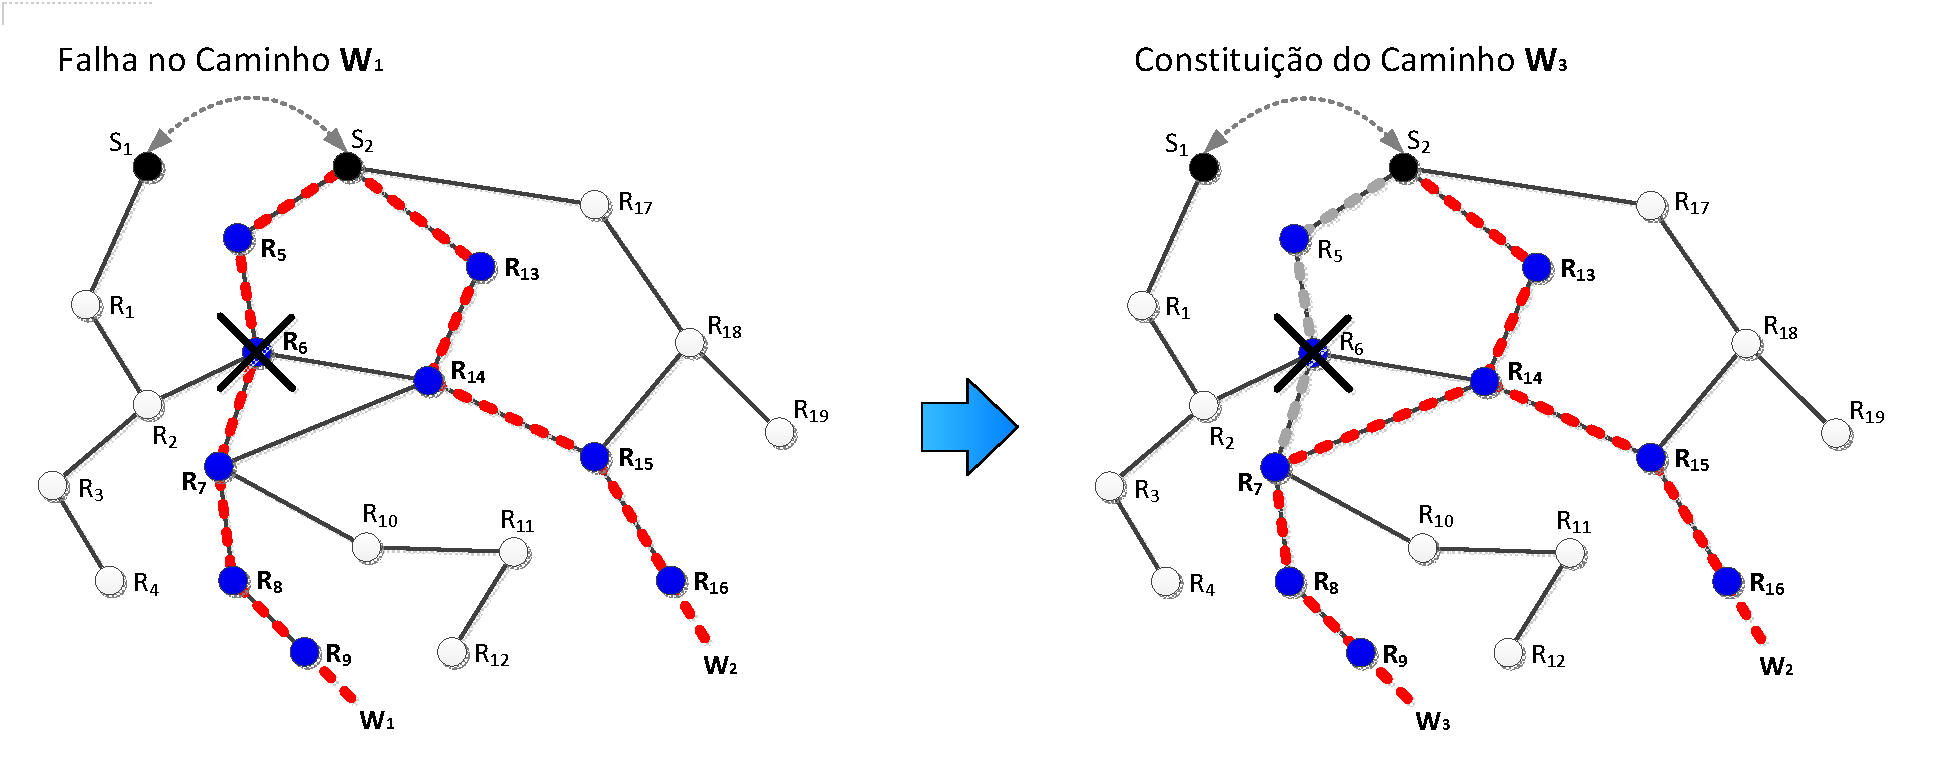
\includegraphics[scale=.5]{imgs/esquema-abstrato-formacao-parceria-intra-falha.pdf}
% \end{center}
% \vspace{-0.8cm}
% \caption{Cen�rio de falha do n� \repassu{6} em um caminho \setwayiu{1}, seguida
% de constitui��o de um novo caminho \setwayiu{3} formado pelo procedimento de
% forma��o de parceria intra \setwayi.}
% \label{fig:esquema-abstrato-formacao-parceria-intra-falha}
% \end{figure}
%
% Al�m da desconex�o expl�cita de um n� \repass, uma a��o espec�fica deve ser
% realizada se um n� \ways $\in$ \setwayis circunstancialmente falhar. Para tratar
% estes casos, definiu-se que o n� \repasss pode formar parcerias com os pr�prios
% n�s \repasss $\in$ \setwayid, tal que \setwayid\space $=$
% \invert{$\delta($\wayu{\wayi+1}, \setwayi$)$}, atrav�s
% de uma outra rota de rede que tamb�m alcance o n� \servs -- isto pode acontecer
% devido � execu��o de algoritmos de roteamento din�mico \textit{Intra-AS
% (Autonomous Systems)}, por exemplo, o OSPF, e \textit{Inter-AS}, por exemplo, o
% BGP~\cite{kurose2006}.
%
% Para entender o comportamento do GMTP em caso de falha de um n� \repass,
% observe a Figura~\ref{fig:esquema-abstrato-formacao-parceria-intra-falha}. Se o
% n� \repassu{6} falhar e o n� \repassu{14} tamb�m estiver repassando \setpk, uma
% nova parceria � formada transparentemente entre o n� \repassu{7} e o n�
% \repassu{14}. Isto porque o n� \repassu{14} interceptar� os pacotes de controle
% de \textit{keep-aline} que o n� \repassu{7} est� transmitindo para o n� \serv.
% Mas, pode acontecer o caso de que \transmitru{14} $ = 0$ e \transmitru{13} $ =
% 0$ para o fluxo de dados \setpk, portanto o pedido de conex�o enviado pelo n�
% \repassu{9} alcan�ar� o n� \servu{1} como antes. Isto resultar� na constitui��o
% de um novo caminho \setwayiu{3} $=$ \setwayidu{1} $\cup$ \setwayidu{2}, tal que
% \setwayidu{1} $=$ \invert{$\delta($\repassu{6}, \setwayiu{1}$)$} e \setwayidu{2}
% $=$ $\delta($\invert{\setwayiu{2}}, \repassu{15}$)$. Isto far� com que todo o
% caminho \setwayiu{3} repasse o fluxo de dados \setpk. Como consequ�ncia,
% aumenta-se a possibilidade de parcerias futuras com n�s \repasss cujo pedido de
% conex�o para obter \setpks seja roteado pelo caminho \setwayiu{3}. Para este
% caso, criou-se o procedimento de forma��o de parceria por intersec��o de
% caminhos \setwayi, detalhado mais adiante.
%
% Na Se��o~\ref{subsec:desconexao}, apresenta-se uma discuss�o geral sobre o
% comportamento do GMTP em outros casos de desconex�es. O procedimento de forma��o
% de parceria intra \setwayi, apresentado nesta se��o, est� intimamente
% relacionado com o processo de estabelecimento de conex�o do GMTP, detalhado mais
% adiante na Se��o~\ref{subsec:conexao-requisicao}.

\subsection{Elei��o de n�s \rel}
\label{subsec:electrelsreps}

Para um fluxo de dados \setpk, o primeiro n� \rels ser� o n� \clis que iniciar a
primeira conex�o para obter o referido fluxo. Os seguintes n�s \rels ser�o os
pr�ximos n�s \clis que se conectar para receber o fluxo de dados \setpk, at�
atingir um par�metro que determinar� a quantidade m�xima de n�s \rels por fluxo
de dados \setpk. Tal par�metro pode ser determinado pelo administrador do n�
\repass. Por padr�o, utiliza-se $\frac{1}{6}$ dos n�s \clis $\in$
\subsetcli$($\repass$)$ como sendo relatores para a transmiss�o de um fluxo
de dados \setpk.

Sendo assim, � medida que um n� \repasss recebe pacotes do tipo
\pac{GMTP-Request}, no pacote de resposta \pac{GMTP-Response}, o n�
\repasss ativa um indicador sinalizando que o referido n� \clis em processo de
conex�o dever� se comportar como um n� \rel, passando a enviar relat�rios
da taxa de transmiss�o calculada, como discutiu-se na
Se��o~\ref{subsec:mudccp-mcc}.

% Note que este modo de transmiss�o deve
% ser implementado com garantia de entrega, ou seja, com a confirma��o de recep��o
% de pacotes e retransmiss�o caso este tipo de pacote seja perdido. Assim, um n�
% \repasss poder� ter controle sobre a quantidade de n�s \rels e receber
% relat�rios apenas dos n�s \rels $\in$ \setrel.

Uma outra situa��o que se faz necess�ria a elei��o de n�s \rels � no
procedimento de desconex�o, como explicado na Se��o~\ref{subsec:desconexao}.
Para esse caso, quando o n� \repasss receber o pacote do tipo
\pac{GMTP-Close}, este deve verificar se o referido n� \clis � um n� \rel. Em
caso afirmativo, o n� \repasss deve transmitir para um dos n�s \clis que
tamb�m recebe o referido fluxo de dados \setpks (se houver), um pacote do tipo
\pac{GMTP-Elect-Request} e aguardar por um \pac{GMTP-Elect-Response}. Este procedimento
deve ocorrer com garantia de entrega.






% Ao \mudccps foi incorporado um mecanismo de toler�ncia a desconex�o que
% funciona de modo a evitar que os clientes deixem de receber dados da
% transmiss�o em quest�o, caso um n� relay desconecte repentinamente sem conseguir
% transmitir um pacote do tipo \mudccp-ElectAck, tal como explicado na
% Se��o~\ref{subsec:mudccp-desconexao}. Considere $T$ uma vari�vel corresponde a
% $4$ vezes o valor do tempo do RTT. Um n� relay deve transmitir no canal de
% controle um pacote do tipo \mudccp-AdvConn a cada instante de $T$, anunciando
% aos demais n�s da rede que est� ativo e operando corretamente. Caso um n� relay
% secund�rio n�o receba o pacote do tipo \mudccp-AdvConn durante o per�odo de
% tempo $T$, assume-se que o relay atual foi desconectado por algum motivo
% desconhecido e o relay secund�rio que n�o recebeu o pacote do tipo
% \mudccp-AdvConn dever� transmitir um pacote do tipo \mudccp-ElectAck. Na
% pr�tica, o n� relay secund�rio torna-se um n� relay prim�rio do o grupo de
% clientes, incluindo os n�s reporters, conectados ao relay que foi desconectado.
% Neste caso, o novo n� relay deve iniciar um novo processo de estabelecimento de
% conex�o. Ap�s o estabelecimento dessa conex�o, como descritos na
% Se��o~\ref{sec:conexaomudccp}, o novo n� relay deve criar o canal de repasse e
% come�a a repassar os dados da transmiss�o multim�dia.


% \subsection{Adapta��o de Fluxo de Dados}
% \label{subsec:adapt-flow}
%
% \begin{figure}[ht]
% \begin{center}
% \includegraphics[natwidth=794,natheight=170,scale=.73]{imgs/bucket-brigade-principle-2.png}
% \end{center}
% \vspace{-0.8cm}
% \caption{Uma aplica��o pode n�o ter recurso suficiente, adapta��es devem ser realizadas.}
% \label{fig:bucket-brigade-principle-2}
% \end{figure}
%
%
% Uma funcionalidade peculiar do \mudccps � sua capacidade de permitir a
% realiza��o de adapta��o de fluxos multim�dia de forma distribu�da. A maioria
% das solu��es para transmiss�o de dados multim�dia, al�m de realizar controle
% de congestionamento em n�vel de aplica��o, realizam adapta��o de fluxo
% multim�dia na fonte geradora dos dados. Em diversas solu��es
% existentes, os autores consideram a transmiss�o de fluxos de dados multim�dia
% adaptados e transmitidos em diferentes canais, sendo que em cada canal
% transmite-se os fluxos multim�dia em uma determinada qualidade. Dependendo da
% qualidade desejada pelo n� receptor, o sistema cliente solicita a transmiss�o em
% um determinado canal. O problema dessa abordagem � que o n� transmissor,
% necessariamente deve transmitir os dados em m�ltiplos canais, o que aumenta a
% complexidade da aplica��o e a quantidade de fluxos de dados sendo transmitidos a
% partir do servidor.
%
% No \mudccp, � poss�vel realizar a adapta��o de fluxo de dados de forma
% distribu�da, na pr�tica, em cada relay. Por exemplo, considere duas redes
% adjacentes, rede 1 e rede 2. Considere que existe um n� relay na rede 1 e entre
% a rede 1 e o n� transmissor a largura de banda de transmiss�o dispon�vel seja de
% \ut{100}{Mbps}. Caso a largura de banda dispon�vel na rede 2 seja de no
% m�ximo \ut{10}{Mbps}, um n� receptor na rede 2 teria que solicitar um fluxo
% multim�dia em um canal diferente, considerando as solu��es que adotam a
% estrat�gia de adapta��o de fluxo com o uso de m�ltiplos canais de transmiss�o.
% No caso do \mudccps � poss�vel que um n� na rede 2 obtenha o fluxo multim�dia
% atrav�s do relay presente na rede 1, com o relay da rede 1 adaptando o fluxo
% multim�dia de acordo com a capacidade do canal de transmiss�o dispon�vel para a
% rede 2. Desta forma, pode-se diminuir o tr�fego na rede do n� transmissor e
% ainda permitir que n�s em redes com largura de banda limitada consigam obter o
% fluxo multim�dia adaptado (caso mais comum para clientes residenciais).
%
%
%
%
%
%
%
%
%
%
% Com essa estrat�gia, fica �bvio que quanto mais requisi��es de
% \textit{pull} por uma parte da m�dia, mais urgente � o seu conte�do para
% reprodu��o. Muitas requisi��es via \textit{pulling} � um sinal que a rede n�o
% est� sendo capaz de entregar \pks t�o r�pido quanto o suficiente para permitir
% a reprodu��o sem que haja interrup��es. Essa informa��o pode ser utilizada para
% adaptar o fluxo de dados \setpk, reduzindo-se sua qualidade e consequentemente
% exigindo menos da rede.
%
%
%
%
%

% \section{Implemeta��o e Implanta��o}
% \label{sec:impl}
%
% PROVER API PARA SETAR AS INFOS DO SDP
%
% O \mudccp\space n�o necessita explicitamente da instala��o de um n� na rede para
% encaminhar o conte�do de uma rede externa para uma rede interna
% (\textit{proxy}). Al�m disso, o \mudccp\space mant�m a \textit{interface} de
% programa��o com a camada de aplica��o inalterada, apenas adicionando uma
% extens�o na API padr�o de \textit{socket} BSD para preservar a compatibilidade
% com as aplica��es multim�dia existentes e, ao mesmo tempo, permitir que as
% aplica��es fa�am uso dos novos recursos do \mudccp. Esta decis�o pode ajudar em
% uma r�pida ado��o do GMTP nas aplica��es multim�dia, permitindo-se simples
% altera��es das aplica��es existentes e, ao mesmo tempo, a efetiva padroniza��o
% da forma como algumas funcionalidades hoje em dia s�o implementadas.


% \section{Benef�cios, Aplicabilidade e Justificativas}
% \label{sec:benef}


%\subsection{Sele��o de Parceiros e de \textit{Chunks}}

% \subsection{Balanceamento de Carga}
%
% Um outro aspecto interessante do protocolo \mudccps � sua capacidade em
% permitir divis�o de carga entre n�s relays. Como os n�s relays recebem e
% repassam os fluxos de dados oriundos de um servidor, obtem-se natualmente uma
% solu��o de distribui��o de conte�do multim�dia sem sobrecarregar a fonte
% geradora de dados (geralmente o servidor). Por�m, mesmo considerando o
% mecanismo atualmente empregado no \mudccps para divis�o de carga entre n�s
% relays, atualmente estuda-se um mecanismo complementar de balanceamento de
% carga a fim de evitar que os n�s relays entre em colapso de congestionamento
% devido ao grande n�mero de clientes conectados a um determinado n� relay.
%
% Considerando isso, est� em estudo no contexto do protocolo \mudccps um
% mecanismo
% de balanceamento de carga que quando um n� relay possui muitas conex�es de
% clientes permite-se que outro cliente seja... PROBLEMA: UM RELAY POR REDE!


% \subsection{Outra Estrat�gia para Descoberta de N�s Relays}
% \label{sec:arcdescorels}
%
% Um aspecto primordial do \mudccps � a capacidade de obter fluxos de
% dados multim�dia atrav�s de n�s relays, os quais repassam esses dados vindo de
% uma fonte geradora. No processo de conex�o, esses n�s relays s�o encontrados,
% aceitam conex�es de clientes e repassam dados da aplica��o como se fossem o
% servidor. Um gargalo no procedimento padr�o adotado no \mudccps � que pode-se
% demorar at� que um cliente \mudccps encontre um n� relay e comece a receber o
% fluxo de dados desejado devido ao mecanismo de busca por profundidade por n�s
% relays utilizando transmiss�es \textit{multicast}, utilizando-se valores incrementais
% para o campo de TTL presente no cabe�alho IP.
%
% Diante disso, est� em estudo no contexto desse trabalho um mecanismo alternativo
% para permitir que um cliente encontre um n� relay mais rapidamente. Este
% mecanismo consiste em permitir que um cliente solicite diretamente ao n�
% servidor a lista de n�s relays conectados a ele, ou seja, a lista dos n�s
% relays de primeiro n�vel (Figura~\ref{fig:cenario-global-detailed}).
%
% O mecanismo de busca por n�s relays permitir� que o cliente consulte, ao longo
% dos n�veis dos n�s relays, aquele n� relay que mais se adequa aos requisitos da
% aplica��o, principalmente com rela��o ao atraso observado desde do servidor at�
% um determinado relay. Um cliente que desejar solicitar esse tipo de
% requisi��o, utiliza o pacote do tipo \mudccp-RelayQuery e transmite o pedido de
% consulta ao servidor, o qual responde ao cliente com a lista dos n�s relays
% de primeiro n�vel utilizando o pacote do tipo \mudccp-RelayReply. Com isto, �
% poss�vel encontrar um melhor relay cujo atraso n�o ultrapasse um determinado
% limiar de tempo definido pela aplica��o, o que n�o necessariamente ser� o n�
% relay mais pr�ximo geograficamente do cliente.



% , dentre
% outros referenciados em~\cite{REF, REF, REF, REF, REF}.

% discutir aqui sobre o que o protocolo tr�s de bom para as aplica��es
%
% - cloud computing
%
% - transmiss�o de casa
%
% - vod
%
% - youtube/copa america
%
% - twitcam

% \section{Outros Aspectos Importantes do \mudccp}
%
% \subsubsection{Uso do Campo \textit{Offset} de Dados}
%
% \subsubsection{Uso do Campo \textit{CCVal} de Dados}
%
% \subsubsection{Soma de Verifica��o e Valida��o de Pacotes}
%
% \subsection{Compatibilidade com outras recomenda��o da IETF}
%
% - NAT - http://www.brynosaurus.com/pub/net/p2pnat/
% - 4340
% - GERA��O DO N�MERO DE SEQU�NCIA
% - RFC2365
% - RFC4086
% - RFC2119
% - TFMCC 4654
% - 5166
% - TFRC 3448

%\section{Considera��es sobre redes de distribui��o de conte�do}

%\section{Considera��es sobre a escolha do DCCP como base para o \mudccp}

\section{Sum�rio do Cap�tulo}
\label{sec:sumario-gmtp}

Neste cap�tulo, apresentou-se o \textit{Global Media Transmission Protocol} (\mudccp), um protocolo baseado em uma arquitetura h�brida P2P/CDN para distribui��o de m�dias ao vivo atrav�s da Internet. Para viabilizar a distribui��o de um fluxo de dados, uma aplica��o obt�m o conte�do e requisita sua transmiss�o ao protocolo GMTP, por meio de uma API \textit{socket}. Para disseminar o conte�do da aplica��o, o GMTP utiliza servidores dispostos em uma rede CDN e constitui dinamicamente uma rede P2P, formada pelos roteadores localizados entre os clientes interessados em obter o fluxo de dados multim�dia e os servidores da CDN. Para isto, os roteadores expressam interesse em participar da rede ao realizarem registros de participa��o (previamente ou sob-demanda) em um ou mais servidores, ao passo que os servidores come�am a conhecer todas as poss�veis rotas para alcan�ar os clientes.

Quando um cliente requisita um fluxo de dados a um servidor, seu roteador de borda, participante da rede P2P, assume a responsabilidade de obter o fluxo de dados de interesse. Nesse �nterim, o roteador do cliente transmite um pedido ao servidor e receber como resposta os pacotes de dados referentes � m�dia de interesse (em modo \textit{unicast/push}). � medida que transmiss�es diretas (servidor $\rightarrow$ cliente) ocorrem, os roteadores presentes nas rotas entre o servidor e os clientes v�o sendo ``alimentados'' pelos pacotes de dados referentes � m�dia em quest�o, ao passo que os roteadores intermedi�rios interceptam os mesmos pacotes de dados quando seus clientes locais tamb�m t�m interesse pela mesma m�dia. Isso habilita o conceito de sub-fluxo.

Os roteadores formam parcerias entre si, diretamente por intercepta��o de pacotes de dados ou com base em instru��es obtidas atrav�s dos servidores, que executam um algoritmo para determinar a intersec��o de rotas usadas por outros roteadores para obter o mesmo fluxo a partir do servidor. Isto ocorre quando o servidor detecta pontos comuns nas rotas e, em vez de aceitar um novo pedido de conex�o de um n� solicitante em obter o fluxo de dados, recusa-o e sugere ao n� solicitante uma lista de roteadores candidatos a parceiros, de modo a evitar m�ltiplas conex�es em dire��o ao servidor. Um roteador pode tamb�m solicitar explicitamente uma lista de candidatos a parceiros a fim de obter mais rapidamente os pacotes de dados e, secundariamente, conhecer outros roteadores e contata-los em caso de desconex�es dos seus parceiros atuais.

A distribui��o do conte�do em uma rede local sempre ocorre em modo \textit{multicast}. Para isto, o roteador cria dinamicamente canais \textit{multicast} e os divulga na rede � medida que recebem pedidos de conex�o para obter fluxos de dados que j� est�o sendo recebidos. Sendo assim, n�o se transmite mais de um pedido de conex�o ao servidor para uma mesma m�dia, partindo da mesma rede. O GMTP executa tr�s fases de conex�o. A primeira fase de conex�o ocorre quando o primeiro n� em uma rede local solicita receber um determinado fluxo de dados; a segunda fase ocorre atrav�s do compartilhamento dos pacotes de dados de um fluxo em modo \textit{multicast}; e a terceira fase permite que os roteadores aumentem suas parcerias.

Em seguida, discutiu-se sobre a estrat�gia para realizar controle de congestionamento durante o processo de dissemina��o de uma m�dia ao vivo. Nesse contexto, prop�e-se dois algoritmos. O GMTP-UCC tem como objetivo controlar o congestionamento no n�cleo da rede P2P, al�m de expor as informa��es de seu estado aos servidores. Os servidores podem utilizar tal informa��o para adaptar o conte�do multim�dia de acordo com a capacidade de transmiss�o da rede, que sempre tende a ser pr�xima da capacidade de um PS. Al�m disso, o algoritmo GMTP-UCC pode auxiliar os n�s receptores a selecionarem os melhores parceiros de acordo com a capacidade de transmiss�o do canal entre os receptores e os transmissores. J� o GMTP-MCC tem como objetivo controlar o congestionamento na rede local, em transmiss�es dos fluxos de dados \textit{multicast}. O roteador elege um sub-conjunto de clientes (relatores) respons�veis por enviar relat�rios de suas respectivas capacidade de recep��o de dados, ao passo que o roteador define a pr�xima taxa de transmiss�o com base nesses relat�rios. Por utilizar uma estrat�gia adaptada do TFRC, o GMTP-MCC emula a taxa de transmiss�o que seria utilizada pelo TCP caso este fosse utilizado para transmitir o fluxo de dados, tornando o GMTP um protocolo TCP-Friendly.

Por fim, discutiram-se aspectos sobre seguran�a e os m�todos empregados no GMTP para evitar ataques de polui��o. O mecanismo de seguran�a do GMTP permite que os servidores assinem digitalmente os dados transmitidos, ao passo que se permite aos repassadores validarem se tal conte�do n�o foi alterado ao longo do caminho entre o servidor e os diversos clientes. Al�m disso, discutiram-se outros aspectos relacionados ao GMTP, como as a��es realizadas na desconex�o dos repassadores, relatores e clientes, bem como a elei��o de relatores.

As defini��es das fun��es do GMTP foram propostas com base em investiga��es dos trabalhos dispon�veis no estado da arte e guiadas por questionamentos sobre quais fun��es se mostraram eficazes ao longo de 15 anos de pesquisa quando aplicadas em sistemas P2P e P2P/CDN, bem como aquelas que podem ser aprimoradas (ou ainda, aquelas que fazem sentido manter na camada de aplica��o). Com esta vis�o, decidiu-se reduzir as responsabilidades dos clientes e aumentar a responsabilidade dos roteadores de rede no processo de dissemina��o dos pacotes de dados multim�dia, fazendo uso de informa��es mais precisas sobre a capacidade de transmiss�o do n�cleo da rede e abstraindo-se a complexidade desse processo da camada de aplica��o. Consequentemente, padroniza-se a forma como as aplica��es distribuem e recebem conte�dos multim�dia, permitindo-se que aplica��es, desenvolvidas por diferentes fornecedores, possam cooperar entre si para obter um mesmo conte�do multim�dia de interesse.

A decis�o de utilizar roteadores para formar uma rede colaborativa, a fim de disseminar o conte�do multim�dia, pode melhorar o desempenho das transmiss�es de conte�dos multim�dia ao vivo, pois reduz-se o impacto negativo causado por fatores que desestabilizam a rede e a qualidade de servi�o, tais como a capacidade de processamento e mem�ria dos dispositivos, mobilidade e din�mica de entrada/sa�da dos clientes (\textit{churn}). Esses fatores s�o os mais cr�ticos em se utilizar uma rede P2P para distribui��o de conte�dos multim�dia, principalmente com a populariza��o dos dispositivos m�veis. Por exemplo, usar dispositivos m�veis como n�s contribuidores de recurso n�o � uma estrat�gia apropriada, principalmente em redes h�bridas IP/celular (por exemplo, 3G). A partir do uso do GMTP, bastar� posicionar um roteador GMTP entre a rede IP e a rede celular para atender � demanda de todos os n�s m�veis.

% No pr�ximo cap�tulo, apresentam-se os resultados e discuss�es acerca do uso do protocolo GMTP para a distribui��o de conte�dos multim�dia ao vivo.
%%%\chapter{Implementa��o do MU-DCCP}

\section{}


%%%\chapter{Experimentos e Estudo de Desempenho do DCCP}

\section{}


% \chapter{An�lise de Projeto e Desempenho do \mudccp}
\label{cap:analisedesemp}

% ====
% 
% * Qual � a diferen�a entre um ensaio, uma simula��o e um experimento?
% * Melhores pr�ticas em design de experimentos sugerem 20 (ou 10 ou 5) experimentos para estimar o desvio padr�o da popula��o inicialmente.
% 
% * Me parece que o racioc�nio na p�gina 105 est� errado. � poss�vel construir um intervalo de confian�a de 95\% para a m�dia de uma popula��o com qualquer quantidade de amostras. O que � o intervalo de confian�a de 95\% sendo constru�do na equa��o 5.11?
%      - Me parece que � um IC com largura igual a 10\% do valor da m�dia. O texto estaria ent�o conceitualmente errado.
% 
% * N�o entendi o experimento: a impress�o que d� � que ele compara a transmiss�o em �rvore vs. uma transmiss�o centralizada. O DCCP tem que ser usado de maneira cliente-servidor? Se n�o, a compara��o � absolutamente injusta. Os experimentos deveriam considerar dois sistemas P2P, um implementado com GMTP e outro com DCCP, n�o? Agora parece uma compara��o de multicast vs. unicast, que j� foi feita 20 anos atr�s.
%      - N�o � bem assim! O GMTP n�o usa multicast exclusivamente
%      - Dizer que o Denacast faz multicast local tb
% 
% * p15: Voc� diz que o DCCP n�o � escal�vel: o problema me parece ser na arquitetura que voc� usou, e n�o no protocolo ponto-a-ponto. Ele pode ser usado para implementar uma mesh.
%      - Sim! Tenho que mudar essa vis�o. O cara pode fazer P2P com DCCP. OK! Ent�o o foco � investir no papo de que o P2P com GMTP est� na infraestrutura, escalar est� na ess�ncia do protocolo, ao passo que usar outros protocolos isso deve ser feito individualmente. OK! Mas o cara pode querer ter flexibilidade na aplica��o, a� faz sua pr�pria solu��o e perde tudo o que o GMTP pode oferecer. Alternativamente, o cara pode fazer um novo GMTP-Intra e aproveitar tudo dispon�veis no GMTP-Inter.
% 
% * p16 (fim): controlar o congestionamento e evitar a trag�dia dos bens comuns n�o � a mesma coisa?
%      - 
% 
% * p17: na sua tese, o que seria um resultado que a negaria? Ela n�o pode ser �bvia.
%      - Um protocolo que comprovasse fazer melhor do que o GMTP considerando apenas a comunica��o end-to-end, com suporte a controle de congestionamento (o que mais??)
%      - Sele��o de n�s � importante
% 
% * Eu entendo que a implementa��o � meio e n�o fim na sua tese. N�o devia ser um objetivo. O objetivo n�o seria obter uma solu��o para um problema X com propriedades Y, Z e W?
%      - Revisar se o papo na introdu��o est� com essa cara
% 
% * N�o entendi o experimento: a impress�o que d� � que ele compara a transmiss�o em �rvore vs. uma transmiss�o centralizada. O DCCP tem que ser usado de maneira cliente-servidor? Se n�o, a compara��o � absolutamente injusta. Os experimentos deveriam considerar dois sistemas P2P, um implementado com GMTP e outro com DCCP, n�o? Agora parece uma compara��o de multicast vs. unicast, que j� foi feita 20 anos atr�s.
%      - Concordo!
% 
% No planejamento:
%      - � necess�ria uma fase de experimentos de simula��o para explorar e justificar as decis�es de design, par�metros e permitir o estudo da contribui��o do trabalho
% 
% ====

Neste cap�tulo, apresentam-se as an�lises do projeto e do desempenho do GMTP para distribui��o de m�dias ao vivo. Na Se��o~\ref{sec:analisedeproj} (an�lise do projeto), generaliza-se a discuss�o acerca dos servi�os disponibilizados no GMTP em compara��o �queles implementados nos principais sistemas. Na Se��o~\ref{sec:analisedesemp} (an�lise de desempenho), estabelecem-se confrontos entre uma implementa��o de refer�ncia do GMTP, o Denacast/CoolStreaming e o CCN/TV, em um ambiente de simula��o que proporcionou a obten��o de valores para as m�tricas avaliadas em um cen�rio que simula parte da Internet. Por fim, na Se��o~\ref{sec:resdisc-sumario}, apresenta-se o sum�rio deste cap�tulo.

Com essa estrat�gia, possibilita-se aprofundar o entendimento sobre o GMTP em duas vertentes (projeto e desempenho), estudando-o por meio de diferentes configura��es de rede e identificando-se suas vantagens e limita��es em compara��o ao estado da arte e da pr�tica.

\section{An�lise do Projeto GMTP}
\label{sec:analisedeproj}

% \subsection{GMTP na Rede Nacional de Pesquisa (RNP)}
% \label{subsec:gmtp-rnp}
% 
% O \textit{backbone} da RNP � estruturado em 27 roteadores distribu�dos em todos os estados brasileiros e foi projetado para garantir n�o s� a largura de banda necess�ria ao tr�fego de Internet usual (navega��o web, correio eletr�nico, transfer�ncia de arquivos), mas tamb�m o uso de servi�os e aplica��es avan�adas e a experimenta��o. A rede possui ramifica��es para atender mais de 500 institui��es de ensino e pesquisa em todo o pa�s, beneficiando mais de 3,5 milh�es de usu�rios.
% 
% A capacidade agregada da RNP � de \ut{233,2}{Gbps}, com velocidades multigigabits ($\ge$ \ut{2}{Gbps}) em 24 dos 27 roteadores (Figura~\ref{fig:rnp-mapa-br}). No contexto internacional, a RNP tem uma conex�o de \ut{1,45}{Gbps} com a Coopera��o Latino-Americana de Redes Avan�adas (RedCLARA), que integra 15 pa�ses da Am�rica Latina e \ut{20}{Gbps} com a Academic Network at S�o Paulo (ANSP). Por meio da uma opera��o em parceria com a ANSP, a RNP se conecta a outras infraestruturas acad�micas internacionais, como � Internet2, � europeia G�ant e � Internet comercial mundial.
% 
% \begin{figure}
% \begin{center}
% \includegraphics[natwidth=1061,natheight=928,scale=.34]{imgs/rnp-mapa-br.png}
% \end{center}
% \vspace{-1cm}
% \caption{Capacidade dos enlaces e pontos de presen�a da RNP no Brasil.}
% \label{fig:rnp-mapa-br}
% \end{figure}
% 
% Na Figura~\ref{fig:rnp-backbone}, ilustram-se detalhes do \textit{backbone} da RNP. Por exemplo, 
% 
% \begin{figure}
% \begin{center}
% \includegraphics[natwidth=664,natheight=340,scale=.61]{imgs/rnp-backbone.png}
% \end{center}
% \vspace{-1cm}
% \caption{\textit{Backbone} da Rede Nacional de Pesquisa (RNP). 27 pontos de presen�a, um em cada estado brasileiro, com 22 pontos de troca de tr�fego. Extra�da de http://www.rnp.br/.}
% \label{fig:rnp-backbone}
% \end{figure}

% Nesta se��o,
% % organiza-se a discuss�o sobre o projeto GMTP em duas partes. Na Se��o~\ref{subsec:gmtp-rnp}, discute-se o funcionamento do GMTP se fosse posto em funcionamento em uma grande rede, instanciando-se a Rede Nacional de Pesquisa (RNP). E, na Se��o~\ref{subsec:gmtp-servicos},
% examinam-se os servi�os do GMTP oferecidos aos sistemas de distribui��o de m�dias ao vivo com vistas aos atuais recursos implementados de forma paliativa nos sistemas existentes, devido � inexist�ncia de um suporte mais efetivo das redes atuais.

No Cap�tulo~\ref{cap:introducao}, questionou-se sobre a real necessidade de diversos recursos implementados nos sistemas para suprir servi�os de rede inexistentes nas camadas inferiores. Em seguida, no Cap�tulo~\ref{cap:fundamentacao}, discutiram-se as abordagens geralmente adotadas nos sistemas de distribui��o de m�dias ao vivo e, de forma similar, o mesmo foi feito no Cap�tulo~\ref{cap:trabalhosrelacionados}, instanciando-se as principais propostas do estado da arte.

Neste cap�tulo, especificamente nesta se��o, objetiva-se justificar a proposta do GMTP n�o apenas como um protocolo com o apelo de reduzir a complexidade dos recursos disponibilizados na camada de aplica��o, mas tamb�m discutir que um conjunto m�nimo de servi�os, quando organizados de forma mais apropriada (nas camadas inferiores), tornam-se equivalentes aos recursos dos atuais sistemas e ainda possibilitam melhorias substanciais tanto no projeto da aplica��o quanto no uso dos recursos de rede.

% \begin{figure}
% \begin{center}
% \includegraphics[natwidth=664,natheight=340,scale=.61]{imgs/gmtp-servicos-sistemas.png}
% \end{center}
% \vspace{-1cm}
% \caption{\textit{Backbone} da Rede Nacional de Pesquisa (RNP). 27 pontos de presen�a, um em cada estado brasileiro, com 22 pontos de troca de tr�fego. Extra�da de http://www.rnp.br/.}
% \label{fig:gmtp-servicos-sistemas}
% \end{figure}

Com esse norte e organizando a discuss�o de acordo com a Figura~\ref{fig:gmtp-servicos-sistemas}, enumeram-se $7$ principais benef�cios promovidos pelo GMTP tanto aos sistemas de distribui��o de m�dias ao vivo e quanto �s redes, relacionando-os com os recursos atualmente empregados na camada de aplica��o.

\begin{itemize}

  \item \textit{Conex�o multi-ponto e tratamentos de diferentes topologias:} Nos sistemas existentes, tratam-se aspectos de conex�o multi-ponto 

  \item \textit{Sele��o de n�s:} 

  \item \textit{toler�ncia a desconex�es e outros problemas causados pelo \textit{churn}}: 

  \item \textit{disponibiliza��o de informa��o de contexto sobre rede para dar suporte � execu��o dos servi�os das aplica��es, como localiza��o da rede, medi��es e custos entre redes para melhorar a qualidade de servi�os dos sistemas finais:}

  \item \textit{estrat�gias para incentivos � coopera��o entre n�s:}

  \item \textit{algoritmos para inibir a participa��o de n�s \textit{free-riders}:}

  \item \textit{adapta��o de fluxo baseado na capacidade de recep��o dos n�s:} 

  \item \textit{seguran�a:}

\end{itemize}

across differents administratives domain
traffic isolation
sem precisar considerar IGP, BGP etc? ler a respeito
diffserv? qual � o outro mesmo? mencionar na problem�tica?


futuro: estudar gmtp + anycast?

\begin{enumerate}

  \item \textit{Otimiza��o arquitetural:} das aplica��es existentes... cliente/servidor, p2p/cdn... usar a palavra autom�tico para cria��o de canais multicast, inclusive entre diferentes dom�nios administrativos, uso transparente de estrat�gias de redes de favores e cdn

  \item \textit{Interoperabilidade entre sistemas:} conex�o, unifica... unifica as aplica��es clientes no ponto de vista do processo de conex�o e obten��o dos dados, uma vez que todo esse processo ocorre na camada de transporte sem qualquer influ�ncia da aplica��o. Isto significa que se existir um n� executando um cliente do sistema PPLive e um outro cliente do sistema SopCast, portanto desenvolvido por equipes diferentes, ambos ainda sim ser�o compat�veis e capazes de cooperar entre si na obten��o do fluxo de m�dia de interesse comum.

  \item \textit{Facilidade na integra��o:} das aplica��es existentes... falar da api socket

  \item \textit{Melhor utiliza��o dos recursos de rede:} controle de congestionamento assistido pela rede, trag�dia dos bens comuns...

  \item \textit{Flexibilidade de uso:} gmtp-inter gmtp-intra extensibilidade

  \item \textit{Elimina��o de recursos paliativos e fen�menos consequentes:} das aplica��es por qu�? pegar a lista abaixo e meter o pau!

  \item \textit{Generaliza��o de boas pr�ticas e abstra��o da complexidade:} citar o que era de aplica��o e foi pra dentro do GMTP

\end{enumerate}

- isso � t�o verdade que na pr�xima se��o ser�o comparadas uma aplica��o gmtp, com um sistema proeminente atualmente e um sistema que segue uma proposta de uma arquitetura futura da internet.

Sendo assim, o que resta para a aplica��o? replicar conteudo nos servidores da cdn e estrat�gias para acessa-los (load balancing etc)

acho que seria muito bom colocar a QeA aqui, n�o desistir f�cil dessa ideia, pois trar� mais robustez a essa se��o. Colocar aqui dentro ou l� no final desse cap? ou nas concls?

- O GMTP n�o � um protocolo multicast fim-a-fim, mas usa multicast na rede local: evitar problemas de integra��o

\section{An�lise de Desempenho do GMTP}
\label{sec:analisedesemp}

PENSAR EM ALGUM GR�FICO PARA COLOCAR L� NA PROBLEM�TICA?

\subsection{Metodologia}
\label{subsec:metodologia}

Nesta se��o, apresentam-se os detalhes dos experimentos realizados. Tais experimentos consistiram de simula��es realizadas no simulador OverSim~\cite{oversim2014} com base no OMNet++~\cite{XU2011,omnetpp2014}, um arcabou�o para constru��o de simuladores de rede. O OverSim possibilita a simula��o de redes e de aplica��es P2P, contendo diversos modelos de protocolos de sobreposi��o: estruturados (por exemplo, Chord, Kademlia e Pastry) e n�o-estruturados (por exemplo, GIA). Sobre essa infraestrutura, utilizou-se a implementa��o do sistema Denacast/CoolStreaming~\cite{denacast2014} e implementou-se o protocolo GMTP e uma aplica��o de refer�ncia~\cite{gmtp2014}. Considera-se uma compara��o  equ�nime porque o Denacast estende o funcionamento do CoolStreaming para dar suporte a uma estrutura h�brida P2P/CDN no processo de distribui��o de m�dias ao vivo atrav�s da Internet, ao passo que o GMTP essencialmente segue o mesmo modelo arquitetura.

\subsection{Objetivo}

O principal objetivo desse estudo foi analisar os valores obtidos das principais m�tricas que determinam a qualidade de servi�o em sistemas de distribui��o de m�dias ao vivo, confrontando-se o desempenho do Denacast/CoolStreaming e do GMTP.

Quebrar a hip�tese da tese em v�rios aspectos

\subsection{Defini��o das Vari�veis (M�tricas)}

Com esse norte, delimitou-se algumas m�tricas que determinam a qualidade de
servi�o para permitir que os usu�rios assistam conte�do ao vivo na Internet
com base na refer�ncia~\cite{5343509}. Tais m�tricas s�o divididas em tr�s
grupos, detalhados a seguir:

\begin{enumerate}

 \item \textit{Qualidade da experi�ncia do usu�rio:} avalia-se o tempo em que os n�s levam para come�ar a reproduzir os primeiros datagramas; o �ndice de continuidade; e a qualidade do conte�do recebido em compara��o ao conte�do original.

 \item \textit{Escalabilidade dos sistemas com rela��o a quantidade de n�s conectados:} avalia-se a quantidade de n�s simult�neos conectados, a contribui��o da rede CDN e da rede P2P na transmiss�o de um fluxo de dados.

 \item \textit{Execu��o dos protocolos:} avalia-se a sobrecarga de controle
gerados pelos protocolos a fim de executar suas fun��es.

\end{enumerate}

M�tricas:
   - Atraso de inicializa��o do fluxo
   - Quantidade de interrup��es
   - �ndice do Continuidade
   - Tempo de recupera��o
   - Distor��o do conte�do recebido em compara��o ao transmitido
   - Sobrecarga de controle
   - N�mero de conex�es no servidor / duplica��es
   - Escalabilidade quanto ao n�mero de n�s clientes interessados por um mesmo fluxo
   - Como posso medir a qualidade das parcerias? pela taxa de transmiss�o entre o n� que compartilha e o n� que recebe
   - Como medir a quantidade de aplica��es de distribui��o de m�dias ao vivo diferentes e a quantidade de eventos iguais sendo transmitidos


Olhar o cap�tulo 4 da tese da nandita para ver os valores dos par�metros que ela usou
ver a p�gina 99 para discuss�es sobre os valores de alfa e beta

\subsection{Defini��o da popula��o}

\subsection{Defini��o da topologia de rede}

\subsection{Defini��o dos experimentos e tratamentos}

\subsection{Considera��es sobre Implementa��o}

Com o intuito de investigar o desempenho do GMTP, implementou-se no simulador de redes OMNet++~\cite{XU2011} suas principais funcionalidades. A vers�o  e sua vers�o atual do protocolo j� permite a execu��o de transmiss�o de dados. Com o
desenvolvimento preliminar do protocolo \mudccps no simulador NS-2, permitiu-se
a execu��o de diversas simula��es a fim de avaliar o comportamento do protocolo
considerando diversas configura��es.

Em linhas gerais, a implementa��o no referido simulador de rede permite a
comunica��o entre os n�s atrav�s dos modos de transmiss�o multicast e unicast.
Foram implementados os tipos de pacotes do \mudccps e os processos de
estabelecimento de conex�o, incluindo o processo de uso de n�s relays, troca
de dados em modos multicast e unicast e os algoritmos para controle de
congestionamento, incluindo o uso de n�s reporters.

Contudo, n�o foi implementado o arcabou�o de extens�o para permitir o
desenvolvimento de novos algoritmos para o processo de conex�o, descoberta e
sele��o de n�s, adapta��o de fluxo de dados e toler�ncia a falhas. Tal
implementa��o ser� feita no n�cleo do sistema operacional Linux, juntamente com
todos os mecanismos b�sicos para o funcionamento do \mudccp.

A proposta � de implementar um arcabou�o de extens�o para as fun��es previstas
no \mudccp, permitindo-se o desenvolvimento e adi��o de novos algoritmos para
as funcionalidades supracitadas, de modo que torne o \mudccps flex�vel para
permitir que qualquer aplica��o os utilizem.

Na pr�tica, um cen�rio desejado para essa proposta de implementa��o do \mudccps
� que o desenvolvedor possa configurar quais algoritmos deseja utilizar em sua
aplica��o, permitindo-se que estes sejam alterados em modo de execu��o da
da mesma. Neste caso, suponha um algoritmo de descoberta de n�s chamado
\textit{DN-1}, um algoritmo para controle de congestionamento chamado
\textit{CC-2}, um algoritmo de toler�ncia a desconex�o \textit{TD-3}; um
algoritmo de adapta��o de fluxo \textit{AF-4} e um algoritmo para reciprocidade
% \textit{R-2}. As implementa��es de tais algoritmos ser�o feitas na camada de
transporte, acoplando-as em forma de m�dulos do sistema operacional ao protocolo
\mudccp. Em seguida, as aplica��es podem selecionar quais algoritmos melhor se
adequa as suas necessidades, com o \mudccps sendo respons�vel por:

\begin{enumerate}

  \item carregar o conjunto de algoritmos \textit{A = \{DN-1, CC-2, TD-3, AF-4,
R-2\}};

  \item definir os par�metros iniciais para cada um dos algoritmos em A,
definidos pela aplica��o;

  \item executar fun��es preliminares para ajustes iniciais, tais como informar
aos n�s participantes de uma transmiss�o quais dos algoritmos est�o sendo
utilizados (o conjunto \textit{A}) e quais outros est�o dispon�veis;

  \item executar os algoritmos em momentos apropriados de acordo com os eventos
de rede, notificando a aplica��o caso necess�rio e desej�vel pela aplica��o;

  \item descarregar os algoritmos quando n�o forem mais necess�rios e informar
aos n�s parceiros.

\end{enumerate}

Desta forma, um n� servidor poder� solicitar que seus n�s clientes carreguem um
determinado m�dulo, dependendo da sua disponibilidade nos n�s clientes. Neste
caso, o \mudccps controlar� todo o processo de carregamento dos mesmos.

Com isso, o \mudccps se tornar� um protocolo extens�vel que gerencia quais
algoritmos devem ser executados em cada ponto de extens�o. Esses algoritmos
podem ser adicionados ao protocolo atrav�s de m�dulos do sistema operacional,
carreg�veis utilizando-se comandos como o \textit{modprobe} (no Linux, por
exemplo) e manipulados (passagem de par�metros) pela aplica��o atrav�s de uma
API de programa��o, por exemplo, utilizando-se as primitivas
\textit{setsockopt()} e \textit{getsockopt()} da especifica��o \textit{BSD
Socket API}~\cite{1197551}.

Para que as aplica��es possam utilizar o \mudccp, o protocolo deve ser
compat�vel com todas as fun��es prevista na especifica��o \textit{BSD Socket
API}, s�o elas: \textit{socket()}, \textit{bind()}, \textit{listen()},
\textit{connect()}, \textit{accept()}, \textit{send()}, \textit{recv()},
\textit{write()}, \textit{read()}, \textit{sendto()}, \textit{recvfrom()},
\textit{close()}, \textit{select()}, \textit{setsockopt()},
\textit{getsockopt()} e \textit{pull()}.

Outros trabalhos podem ser desenvolvidos para tornar o \mudccps compat�vel com o
padr�o de \textit{sockets} do sistema operacional Windows, conhecido pelo nome
de \textit{winsock}. Todavia, por ser um sistema operacional de c�digo fechado,
a implementa��o do \mudccps s� ser� poss�vel ap�s sua padroniza��o em forma de
RFC.



\section{Resultados e Discuss�es}
\label{sec:resdisc}

GMTP vs. CoolStreaming

- Denacast com GMTP, DCCP e UDP
     - Com e sem o RCP
          - Com RCP sem sub-fluxo
          - Com RCP com sub-fluxo
- CoolStreaming com GMTP n�o faz sentido porque transformaria-se o GMTP em uma aplica��o igual a que ser� utilizada para os confrontos

- Lembrar de enfatizar a interoperabilidade em cen�rios reais que o GMTP proporciona. "Arquiteturalmente, o GMTP resolve o problema de permitir a interoperabilidade dos sistemas e otimiza o uso de recursos de rede ..."

- Colocar uma curva que mostra a capacidade da rede e o quanto o GMTP consegue usar?

- Pensar em colocar diversas aplica��es em execu��o no mesmo instante. Isso poderia como um "at a glance" na se��o de problem�tica.

PENSAR NAS VARI�VEIS DEPENDENTES E INDEPENDENTES

TEM QUE DIZER QUE USEI O BRITE

REPENSAR SE AVALIA TAMB�M O CCN-TV OU N�O! SE N�O FOR FAZER ISSO, REVER AS INFORMA��ES NA CAP DE TR SOBRE DETALHAR A COMPARA��O, CASO CONTR�RIO, PENSAR SE DEIXA ESSE ITEM OU TIRA
MANTER O PPSP/Swift? Se sim, rever o que o nazareno colocou sobre isso...


\subsection{M�todos e simula��es}

\subsection{Par�metros de simula��o}

\subsection{Resultados}

\subsection{Discuss�es}

% -----------------


% OS PROTOCOLOS DE TRANSPORTE NAO FORAM PROJETADOS/PENSADOS/PREPARADOS PARA P2P
% VER OUTRAS CARACTER�STICAS DOS SISTEMAS DE DISTRIBUI��O

% FAZER FIGURA DE COMO ESTES PAR�METROS SE RELACIONAM
% startup delay time ->
% recovery period to restart
% content distortion
% vs
% * qualidade das parcerias -> atraso -> pr�-defini��o de rotas (tracer)
% redu��o do churn (oportunismo) -> melhor startup delay time e recovery period
% to restart -> rede p2p constitu�da entre os roteadores -> buffer pequeno e
% expiram rapidamente
%

\section{GMTP vs. CCN-TV}

CCN-TV 6550523

% - http://named-data.net/wp-content/uploads/2013_Yuan_Infocom_Mini.pdf
  Olhar os gr�ficos desse artigo

cite 6607500
cite 6386696

\subsection{M�todos e simula��es}

\subsection{Par�metros de simula��o}

\subsection{Resultados}

\subsection{Discuss�es}

\section{Sum�rio do Cap�tulo}
\label{sec:resdisc-sumario}
% \chapter{Considera��es Finais}
\label{cap:conclusao}

Fazer pacote geral do GMTP

Conclusions are not a rambling summary of the thesis: they are short, concise statements of the inferences that you have made because of your work. It helps to organize these as short numbered paragraphs, ordered from most to least important. All conclusions should be directly related to the research question stated in Section 4. Examples:

1. The problem stated in Section 4 has been solved: as shown in Sections ? to ??, an algorithm capable of handling large-scale Zylon problems in reasonable time has been developed.

2. The principal mechanism needed in the improved Zylon algorithm is the Grooty mechanism.

3. Etc.

TBD

- EVIDENCIAR OS GANHOS DE MOVER ALGUMAS QUEST�ES DE UMA CAMADA PRA OUTRA
- REPENSAR SE COLOCO COMO CONTRIBUI��O O LANCE DO SIMULADOR
- RETOMAR:

\textit{a constitui��o de uma rede de favores entre roteadores que interceptam, realizam cache tempor�rio e compartilham pacotes de dados tanto em modo \textit{multicast} (em redes locais) quanto em modo unicast (entre redes distintas), com o aux�lio de um algoritmo para controle de congestionamento assistido pela rede, possibilita a independ�ncia dos sistemas e o melhor uso dos recursos de rede e, consequentemente, a distribui��o eficiente de fluxos de m�dias ao vivo}.

% \section{Perguntas Frequentes}


\section{Conclus�es}

* Colocar no �ltimo slide da apresenta��o: os direcionamentos sugeridos na qualifica��o foram fundamentais para...

* Falar que o GMTP-Intra pode ser alterado sem impactar no GMTP-Inter e vice-versa. � uma ``falsa'' mistura entre as duas camadas (cross-layer).

* Por que PS? � invariante a distribui��o do tamanho do fluxo, ou seja, n�o importa ao diferentes s�o os tamanhos dos fluxos na rede. Mesmo com longos fluxos, o compartilhamento do canal � melhor porque estabiliza mais r�pido se comparado com abordagens de monitoramento de perdas.
   RCP: atualiza a taxa (simples e pr�tico): aproxima a taxa de transmiss�o oferecida aos fluxos da taxa do PS, sem o conhecimento do n�mero exato de fluxos; baseia-se no tamanho da fila, no tr�fego agregado de entrada e no RTT m�dio do tr�fego passando atrav�s do link
   R(t) � atualizado de acordo com h0.
   Cada roteador tem que fazer tr�s coisas
       - offer the same rate to every flow
       - preencher a fila de sa�da com os pacotes que chegam na fila de entrada
       - manter a fila de entrada e sa�da pequena
   Long-flow: 100\% link utilization
   Short-flow: reduce flow completion time,
   Flash-crownd no RCP: pode ter perde
   A quest�o �: em vez de definir aumentos ou uma diminui��es incrementais na janela com base no RTT, no RCP a pergunta �: existe uma taxa de transmiss�o que os roteadores podem pedir aos fluxos transmitirem e emular o PS. Qual seria essa taxa? como encontr�-la de forma simples?
   Para ter um FCT pequeno, tem que ter alta utiliza��o do link, ent�o precisa-se garantir  que o buffer n�o estoure (rever 28:30min da defesa da Nandita)
   Nem sempre o XCP � ruim, quando s� tem long-lived, mas em cen�rios din�micos (diferentes tamanhos de fluxos) it performs badly and short lived flows last almost the same time of some long lived flows. Quando aumenta o tamanho m�dio do fluxo para se aproximar ao Bandwidth-delay product, you approach the regime where you have a few high Bandwidth flows multiplex in a large link (51:00min)
   Diferentes topologias: 
     - Sem manter estado por fluxo
     - TCP: perda de pecotes ou atraso
     - XCP: alcan�a desempenho similar ou melhor do que HS-TCP para long-lived flows
            n�o � 100\% fair em determinados momentos
            em fluxos mistos (tamanho) e na din�mica da rede n�o � bom
            multiplica��es e divis�es � sim ruim (Nandita -> Cisco)
            
            
     - CC: na literatura, em geral, s� focam em usar o m�ximo do link


\section{Resumo das Contribui��es}
\label{sec:contribuicoes}

The Summary of Contributions will be much sought and carefully read by the examiners. Here you list the contributions of new knowledge that your thesis makes. Of course, the thesis itself must substantiate any claims made here. There is often some overlap with the Conclusions, but that's okay. Concise numbered paragraphs are again best. Organize from most to least important. Examples:

1. Developed a much quicker algorithm for large-scale Zylon problems.

2. Demonstrated the first use of the Grooty mechanism for Zylon calculations.

3. Etc.


No contexto desta tese, resume-se as principais contribui��es.

\begin{enumerate}

%   \item Uma revis�o bibliogr�fica sobre o estado da arte no contexto do
% tema que se discute. Apresenta-se a forma de com os sistemas atualmente s�o
% projetados e as principais considera��es sobre os mesmos, como t�cnicas,
% m�todos e abordagens utilizadas;

  \item a concep��o e descri��o detalhada de um protocolo para distribui��o de conte�dos multim�dia ao vivo. Apresenta-se a elabora��o do GMTP, que considera a comunica��o mais efetiva entre as duas camadas mais importantes da pilha TCP/IP, a de transporte e a de rede.
%   Al�m disso, (re)visita-se assuntos importantes na �rea de redes e traz-se � tona os recentes avan�os da �rea de estudo, como os conceitos das redes centradas na informa��o~\cite{6563278} e os algoritmos de controle de congestionamento assistido pela rede~\cite{983548}.
  Nesse contexto, contribui-se com uma proposta de como pode-se permitir a interoperabilidade dos atuais sistemas de distribui��o multim�dia, promovendo-se formas de adapta��o dos sistemas existentes.
% , bem como o re�so de algumas fun��es comuns a todos os sistemas.

  \item discuss�es sobre a aplica��o do \textit{Rate Control Protocol} (RCP)~\cite{Dukkipati:2008:RCP:1368746} no GMTP. O RCP � um proeminente algoritmo de controle de congestionamento assistido pela rede e foi usado no GMTP para auxiliar no processo de distribui��o de m�dias ao vivo. Nesse contexto, contribui-se com discuss�es sobre as adapta��es realizadas no RCP para permitir sua aplica��o ao GMTP e como se pode utiliz�-lo no processo de forma��o de parcerias em uma rede de favores, fun��o jamais vista em qualquer outra solu��o de distribui��o de m�dias ao vivo. Ou seja, al�m de utilizar o RCP para melhorar o consumo dos recursos compartilhados de rede (controle de congestionamento), prop�e-se um algoritmo de sele��o de n�s parceiros com base na atual capacidade de transmiss�o dos enlaces entre os n�s servidores de um fluxo de dados ao vivo e os n�s clientes interessados em receb�-lo. Ademais, discute-se aspectos fundamentais sobre a escolha do RCP em detrimento a outras propostas bem conhecidas, como o XCP~\cite{Katabi2003} e o VCP~\cite{4460574}.

  \item os resultados e discuss�es acerca do GMTP frente a uma proeminente proposta: o Denacast/CoolStreaming~\cite{5764567}.
%  e o CCN-TV~\cite{6550523}.
O Denacast � um sistema de distribui��o de m�dias ao vivo baseado no CoolStreaming com suporte a uma rede de distribui��o de conte�dos (P2P/CDN). Com os resultados comparativos obtidos, contribui-se para tomada de decis�es sobre futuras pesquisas no contexto de distribui��o de m�dias ao vivo.
% O CCN-TV � um sistema de TV para Internet com suporte �s redes centradas na informa��o. Com isto, contribui-se para tomada de decis�es sobre futuras pesquisas no contexto de distribui��o de m�dias ao vivo.

  \item a implementa��o de artefatos de software que permitem a reprodu��o do ambiente de estudo, tais como implementa��o do GMTP no simulador de rede OMNet++~\cite{XU2011,omnetpp2014}.
%  bem como encaminhamentos iniciais de implementa��o no n�cleo do Linux.

  \item os encaminhamentos da pesquisa sobre futuros avan�os do estado da arte,
tais como as limita��es do protocolo proposto e uma breve discuss�o de como
essas limita��es poder�o ser aprimoradas.

\end{enumerate}

Ademais, destaca-se a import�ncia e originalidade do presente trabalho por ser o primeiro a trazer � tona um problema e uma proposta de solu��o do uso de um protocolo de transporte e rede, exclusivamente projetado para a distribui��o de m�dias ao vivo na Internet. At� ent�o, distribuir conte�dos multim�dia na Internet se resumia em sistemas baseados em protocolos tradicionais (TCP, UDP, DCCP, SCTP) ou outros propriet�rios, em geral, dispon�veis na camada de aplica��o e independentes.

PS: O GMTP vai al�m de uma simples solu��o multicast porque permite a parceria entre diferentes n�s que n�o est�o necessariamente na mesma �rvore multicast.

\section{Limita��es}

- a quebra de fluxos em sub-fluxos requer maior processamento para medi��es de RTT
- implanta��o (ver a tese da dina)
- 

\section{Trabalhos Futuros}

- Considerar outras topologias
- Tr�fego background + impacto no TCP

The Future Research subsection is included so that researchers picking up this work in future have the benefit of the ideas that you generated while you were working on the project. Again, concise numbered paragraphs are usually best.

- montar uma rede e colocar pra funcionar na Internet
- otimizar a obten��o dos n�s em uma rota (pensar sobre como nem sempre colocar o identificador nos pacotes de registro de participa��o). Que tal olhar para o endere�o de destino e fazer cache, em um determinado per�odo de cache n�o p�e mais o identificador. Ser� que funcionar�? como ficam as quest�o de um roteador colocar e outro n�o? ou todos colocam ou nenhuma coloca. Nesse caso, pode-se usar uma flag qd o primeiro n�o colocar.


8. Appendices

COLOCAR CABE�ALHO DOS PACOTES?

REPRODUCIBLE RESEARCH?

What goes in the appendices? Any material which impedes the smooth development of your presentation, but which is important to justify the results of a thesis. Generally it is material that is of too nitty-gritty a level of detail for inclusion in the main body of the thesis, but which should be available for perusal by the examiners to convince them sufficiently. Examples include program listings, immense tables of data, lengthy mathematical proofs or derivations, etc.



\section{An�lise do Projeto GMTP}
\label{sec:analisedeproj}

% \subsection{GMTP na Rede Nacional de Pesquisa (RNP)}
% \label{subsec:gmtp-rnp}
% 
% O \textit{backbone} da RNP � estruturado em 27 roteadores distribu�dos em todos os estados brasileiros e foi projetado para garantir n�o s� a largura de banda necess�ria ao tr�fego de Internet usual (navega��o web, correio eletr�nico, transfer�ncia de arquivos), mas tamb�m o uso de servi�os e aplica��es avan�adas e a experimenta��o. A rede possui ramifica��es para atender mais de 500 institui��es de ensino e pesquisa em todo o pa�s, beneficiando mais de 3,5 milh�es de usu�rios.
% 
% A capacidade agregada da RNP � de \ut{233,2}{Gbps}, com velocidades multigigabits ($\ge$ \ut{2}{Gbps}) em 24 dos 27 roteadores (Figura~\ref{fig:rnp-mapa-br}). No contexto internacional, a RNP tem uma conex�o de \ut{1,45}{Gbps} com a Coopera��o Latino-Americana de Redes Avan�adas (RedCLARA), que integra 15 pa�ses da Am�rica Latina e \ut{20}{Gbps} com a Academic Network at S�o Paulo (ANSP). Por meio da uma opera��o em parceria com a ANSP, a RNP se conecta a outras infraestruturas acad�micas internacionais, como � Internet2, � europeia G�ant e � Internet comercial mundial.
% 
% \begin{figure}
% \begin{center}
% \includegraphics[natwidth=1061,natheight=928,scale=.34]{imgs/rnp-mapa-br.png}
% \end{center}
% \vspace{-1cm}
% \caption{Capacidade dos enlaces e pontos de presen�a da RNP no Brasil.}
% \label{fig:rnp-mapa-br}
% \end{figure}
% 
% Na Figura~\ref{fig:rnp-backbone}, ilustram-se detalhes do \textit{backbone} da RNP. Por exemplo, 
% 
% \begin{figure}
% \begin{center}
% \includegraphics[natwidth=664,natheight=340,scale=.61]{imgs/rnp-backbone.png}
% \end{center}
% \vspace{-1cm}
% \caption{\textit{Backbone} da Rede Nacional de Pesquisa (RNP). 27 pontos de presen�a, um em cada estado brasileiro, com 22 pontos de troca de tr�fego. Extra�da de http://www.rnp.br/.}
% \label{fig:rnp-backbone}
% \end{figure}

% Nesta se��o,
% % organiza-se a discuss�o sobre o projeto GMTP em duas partes. Na Se��o~\ref{subsec:gmtp-rnp}, discute-se o funcionamento do GMTP se fosse posto em funcionamento em uma grande rede, instanciando-se a Rede Nacional de Pesquisa (RNP). E, na Se��o~\ref{subsec:gmtp-servicos},
% examinam-se os servi�os do GMTP oferecidos aos sistemas de distribui��o de m�dias ao vivo com vistas aos atuais recursos implementados de forma paliativa nos sistemas existentes, devido � inexist�ncia de um suporte mais efetivo das redes atuais.


\bibliographystyle{unsrt} % estilo de bibliografia   plain,unsrt,alpha,abbrv.
%\bibliographystyle{plain}
% \bibliographystyle{abnt}
\bibliography{biblio-phd,biblio-master,biblio-zotero}

% \appendix
% % \chapter{Sistemas de Transmiss�o de V�deo P2P}
% \label{apd:survey-video-p2p}
%
% TBD

% http://tools.ietf.org/wg/ppsp/draft-ietf-ppsp-survey/
% surveys/10.1.1.111.3092.pdf
% surveys/draft-ietf-ppsp-survey-02.txt
% surveys/p2pvs.pdf

%\chapter{M�todos, Simula��es e Experimentos}
\label{cap:metodosexperimentos}

% \begin{center}
%     \begin{minipage}{300pt}
%     \small
%     \centering
% 	``Sabemos que uma conclus�o definitiva n�o pode ser feita baseando-se nas caracter�sticas de todos os sistemas, mas � poss�vel obter conclus�es probabil�sticas baseando-se num intervalo onde estar�o as caracter�sticas da maioria dos sistemas.'' (Raj Jain, em \emph{A Arte da An�lise de Desempenho em Sistemas de Computa��o})
%     \end{minipage}
% \end{center}

\vspace{1cm}

Neste cap�tulo � descritos o m�todo estat�stico utilizado para a
obten��o das m�tricas estabelecidas para analisar o desempenho do
protocolo \mudccps e as metodologias adotadas para obten��o dos valores finais
para cada uma das m�tricas obtidas.

Para isto, apresenta-se um m�todo estat�stico baseado na teoria da
probabilidade, que possibilita calcular a quantidade de ensaios necess�rios para
um determinado tratamento de simula��o e assim obter um n�vel de confian�a de
\ut{95}{\%} nos valores apresentados. Com este m�todo, foi poss�vel realizar
compara��es quanto ao desempenho do \mudccps frente a outros protocolos
tradicionais, como o DCCP e o TCP. Tais discuss�es comparativas s�o
apresentadas no Cap�tulo~\ref{cap:analisedesemp}.

% Para entender melhor os conceitos apresentados a seguir, antes � necess�rio
% entender algumas nomenclaturas utilizadas universalmente em pesquisas
% cient�ficas e portanto tamb�m utilizadas neste trabalho. Em pesquisas
% cient�fica, um tratamento � um cen�rio de simula��o definido por uma
% combina��o de fatores. Um fator � um par�metro de configura��o de um tratamento,
% por exemplo a largura de banda ou a taxa de perda de pacotes configurada para
% um determinado canal de transmiss�o simulado. Em cada tratamento deseja-se
% estudar as vari�veis, ou tamb�m chamadas de m�tricas, as quais s�o informa��es
% coletadas e geradas atrav�s da execu��o de um tratamento, por exemplo, a taxa de
% transmiss�o obtida por um determinado protocolo. Por fim, para cada execu��o de
% um tratamento d�-se o nome de ensaio.

\section{Tratamentos}
\label{sec:paramexp}

Neste trabalho, considerou-se a an�lise do protocolo \mudccps em confronto com o protocolo
DCCP e o TCP.

De acordo com os objetivos deste trabalho, considera-se desnecess�ria uma
an�lise de desempenho do \mudccps em confronto com protocolos tradicionais como
o UDP. Isto porque em diversos trabalhos anteriores, inclusive na disserta��o de
mestrado do autor desta proposta de tese~\cite{leandro-master-2008},
j� foram apresentadas avalia��es comparativas entre o DCCP, o TCP e o UDP. No
estado atual, procura-se avaliar o comportamento do \mudccps com rela��o a sua
capacidade de escalabilidade diante de grandes quantidades de n�s receptores e
de sua equidade diante de m�ltiplos fluxos de dados. Por este motivo,
descartou-se a necessidade de avaliar o desempenho do \mudccps em confronto
com o UDP, uma vez que este �ltimo n�o implementa qualquer solu��o para controle
de congestionamento, compartilhamento de conex�o etc.

Para os tratamentos que apresentam resultados do confronto entre o protocolo
\mudccps e o DCCP, cujo principal objetivo � apresentar a capacidade de
escalabilidade de ambos os protocolos, as simula��es foram executadas de forma
isolada, primeiramente o DCCP e em seguida o \mudccp.

O tempo de dura��o da execu��o de cada ensaio foi de \ut{400}{s}, onde cada
ensaio foi repetido a quantidade de vezes necess�rias at� atingir um intervalo
de confian�a de \ut{95}{\%}, de acordo com as defini��es estabelecidas na
Se��o~\ref{sec:metestat}.

% Um outro ponto considerado foi com rela��o ao momento de iniciar cada fluxo. Em
% se tratando das transmiss�o TCP, em qualquer tratamento os fluxos TCP foram
% iniciados primeiro e isoladamente at� os \ut{50}{s} iniciais do ensaio.
% Ap�s esse tempo, fluxos \mudccps foram iniciados. O objetivo para tal
% procedimento foi analisar qualquer impacto gerado pelo \mudccps em
% rela��o a um fluxo de dados TCP.

Definiu-se dois tratamentos, um com confrontos \mudccps vs. DCCP vs. TCP
(Tratamento 1) e o outro com confrontos entre \mudccps vs. DCCP (Tratamento 2).
O objetivo do Tratamento 1 � averiguar a capacidade de converg�ncia e
equidade dos fluxos transmitidos utilizando o \mudccps analizando a vaz�o
obtida por esses fluxos. Por outro lado, o objetivo para o Tratamento 2 �
averiguar a escalabilidade do \mudccps no que diz respeito a quantidade de n�s
receptores interessados em um mesmo fluxo de dados transmitido por um n�
servidor. Esta avalia��o foi realizada aumentando-se a quantidade de n�s
receptores gradativamente em uma transmiss�o de v�deo \mys, coletando-se
valores para as m�tricas de vaz�o, carga de dados transmitida e perda de
pacotes, atraso e qualidade do v�deo transmitido. A metodologia adotada neste
trabalho para obten��o de cada uma das m�tricas mencionadas anteriormente ser�
explicada na Se��o~\ref{sec:metrescdevexp}.

Os Tratamentos $1$ e $2$ foram executados em simula��es de rede
no NS-2~\cite{netsimulator2} cuja topologia da rede foi definida como uma �rvore
bin�ria completa, segundo a Figura~\ref{fig:topologia_rede_metodo_experimento}.
Al�m disso, alguns fatores foram pr�-definidos e s�o descritos a seguir.

\begin{figure}[ht]
\begin{center}
\includegraphics[scale=.7]{imgs/topologia.pdf}
\end{center}
\vspace{-0.5cm}
\caption[Topologia da rede definida para as simula��es com \mudccp, DCCP e
TCP]{Topologia da rede definida para as simula��es realizadas. Cada
rede � representada por um roteador e com 10 n�s em cada rede.}
\label{fig:topologia_rede_metodo_experimento}
\end{figure}

\begin{itemize}
\item N�mero de computadores receptores por rede: 10
\item Largura de banda da rede local: \ut{100}{Mbps}
\item Lat�ncia da rede local: \ut{1}{ms}
\item Largura de banda do backbone: \ut{100}{Mbps}
\item Lat�ncia do backbone: \ut{5}{ms}
\item Tamanho da fila dos roteadores do backbone: \ut{3000}{}pacotes
\item Dura��o da simula��o: \ut{400}{s}
\end{itemize}

De acordo com a topologia definida, cada n� da �rvore representou um roteador,
cada um com $10$ n�s receptores TCP, DCCP e/ou \mudccps conectados a
ele. Para o caso do Tratamento 2, os ensaios foram executados � medida em
que se aumentava o n�vel da �rvore. Por exemplo, $r$ ensaios foram
executados para $10$ n�s receptores e $1$ roteador, pois o n�vel da �rvore
\textit{L} foi igual a $0$ (zero); em seguida $r$ outros ensaios foram
executados utilizando-se $30$ n�s receptores e $3$ roteadores, pois L=1; em
seguida, outros $r$ ensaios foram executados utilizando-se $70$ n�s receptores e
$7$ roteadores, pois L=2; e assim por diante at� L=9, quando utilizou-se
$10.230$ n�s receptores e $1.023$ roteadores. Deve-se utilizar $n=2^{L+1}-1$
para se obter a quantidade \textit{n} de roteadores dado um n�vel \textit{L} da
topologia de rede utilizada.

Os fluxos de dados foram transmitidos da seguinte forma: um n� localizado na
raiz da �rvore transmitiu o mesmo conte�do multim�dia para todos os outros n�s
conectados � rede, simulando uma t�pica transmiss�o multim�dia \mys\space e um
tr�fego de comportamento equivalente a um v�deo MPEG-2.

\section{M�tricas Selecionadas e M�tricas Derivadas}
\label{sec:metrescdevexp}

Com rela��o aos tratamentos que envolveram transmiss�es de fluxos de dados dos
protocolos TCP e \mudccp, foi estudada apenas a m�trica de vaz�o, ao passo que
tratamentos que envolveram a an�lise de desempenho do \mudccps com rela��o do
protocolo DCCP, foram analisadas as m�tricas de vaz�o, perda de pacote e a
lat�ncia, que atrav�s desta �ltima foi poss�vel calcular o \emph{jitter} m�dio
para uma determinada transmiss�o. Al�m disso, atr�ves da vaz�o e da quantidade
de pacotes perdidos, pode-se obter a carga efetiva de dados transmitidos.

Para cada m�trica selecionada, foram coletados seus valores instant�neos e para
cada uma delas algumas considera��es s�o discutidas a seguir.

\subsection{Vaz�o M�dia, Carga Efetiva M�dia, Lat�ncia M�dia e Jitter}
\label{subsec:vazcaglat}

Para um determinado tratamento, a m�dia final da vaz�o e da carga efetiva
transmitida pelo TCP foi obtida atrav�s da m�dia aritm�tica das m�dias das
vaz�es obtidas em cada ensaio \textit{r}, ou seja, atrav�s das
Equa��o~\ref{eq:vazaomediaTCP} e~\ref{eq:cargamediaTCP}, onde \textit{n}
� o total de ensaios de um determinado tratamento. Assim, temos:

\begin{equation}
\mu_{vazaotcp} = \frac{\sum_{r=1}^{n} \fmtvar{vaz�o\_m�dia}_{r}}{n}
\label{eq:vazaomediaTCP}
\end{equation}

\begin{equation}
\mu_{cargatcp} = \frac{\sum_{r=1}^{n} \fmtvar{carga\_m�dia}_{r}}{n}
\label{eq:cargamediaTCP}
\end{equation}

No entanto, para obter as m�dias da vaz�o e carga efetiva dos fluxos \mudccp, o
procedimento foi um pouco diferente. Considerando que os fluxos \mudccps foram
sempre iniciados \ut{50}{s} ap�s o fluxo TCP, � preciso definir um mecanismo que
n�o penalize \mudccp, j� que eles deixaram de transmitir por \ut{50}{s}. Assim,
dado que:

\begin{equation*}
\mu_{\fmtvar{vaz�o}\lmudccp} = \frac{\sum_{r=1}^{n}
\fmtvar{vaz�o\_m�dia}_{r}}{n}
\label{eq:vazaomediaUDDC}
\end{equation*}

\noindent onde $\fmtvar{vaz�o\_m�dia}_{r}$ � obtida atrav�s da m�dia aritm�dia
das vaz�es em cada segundo de cada ensaio, tem-se que a vaz�o para os fluxos do
protocolo \mudccps � obtida atrav�s da Equa��o~\ref{eq:vazaomediafinalUDDC}.

\begin{equation}
\mu_{vazao-final-\mudccp)} = \mu_{\fmtvar{vaz�o}\lmudccp} + S \times
(\frac{\mu_{\fmtvar{vaz�o}\lmudccp}}{T})
\label{eq:vazaomediafinalUDDC}
\end{equation}

Onde,

\begin{itemize}

 \item $S$, o tempo de atraso para iniciar os fluxos UDP ou DCCP
($S=\ut{50}{s}$);

 \item $T$, o tempo total do ensaio ($T=\ut{400}{s}$).

\end{itemize}

Assim, as m�dias s�o normalizadas para n�o penalizar nenhum dos protocolos, com
base na Equa��o~\ref{eq:vazaomediafinalUDDC}.

De forma equivalente, pode-se obter a carga m�dia efetivamente transmitida e da
lat�ncia m�dia. Note que para o confronto \mudccps $\times$ DCCP, a vaz�o
m�dia e carga m�dia s�o obtidas atrav�s das Equa��es~\ref{eq:vazaomediaTCP}
e~\ref{eq:cargamediaTCP}, respectivamente.

\subsubsection*{Jitter}

O c�lculo para obter o valor m�dio do \emph{jitter} para um fluxo transmitido �
bastante similar ao c�lculo da vaz�o m�dia. Este valor pode ser obtido atrav�s
da Equa��o~\ref{eq:jittermediofinalUDDC}. Esta equa��o foi obtida da seguinte
forma:

\begin{equation}
\mu_{\fmtvar{jitter-parcial-\lmudccp}} = \frac{\sum_{r=1}^{n}
\fmtvar{jitter\_m�dio}_{r}}{n}
\label{eq:jittermediaUDDC}
\end{equation}

onde,

\begin{equation*}
\fmtvar{jitter\_m�dio}_{r} = \frac{\sum_{k=1}^{Q} V_k}{Q}
\label{eq:latenciamediarUDDC}
\end{equation*}

Logo,

\begin{equation}
\mu_{\fmtvar{jitter-final-\lmudccp}} = \mu_{\fmtvar{jitter-parcial-\lmudccp}}
+ S \times (\frac{\mu_{\fmtvar{jitter-parcial-\lmudccp}}}{T})
\label{eq:jittermediofinalUDDC}
\end{equation}

Sendo,

\begin{itemize}

 \item $Q$, quantidade de intervalos ($Q = T - 1$) entre cada medi��o do
ensaio, ou seja, entre dois segundos quaisquer consecutivos;

 \item $V$, valor da varia��o do atraso entre pacotes de um mesmo fluxo, por
exemplo para $\fmtvar{instante}_1 = \ut{10,3}{ms}$ e $\fmtvar{instante}_2 =
\ut{11,2}{ms}$, $V = \ut{0,9}{ms}$;

 \item $T$, o tempo total do ensaio ($T=\ut{400}{s}$).

\end{itemize}

\section{Metodologia Estat�stica para o C�lculo Final das M�tricas Estudadas}
\label{sec:metestat}

Os resultados apresentados neste trabalho, por exemplo, para determinar que um
protocolo obteve melhor desempenho que outro em termos da vaz�o m�dia, foram
baseados em amostras dos dados coletados em cada ensaio de um tratamento. A
metodologia adotada baseia-se no conceito de intervalo de
confian�a~\cite{jain1991}, considerando $\rho = \ut{95}{\%}$ (n�vel de
confian�a) e portanto $\alpha = \ut{5}{\%}$ (n�vel de signific�ncia, ou erro).

\subsubsection*{Determinando o Intervalo de Confian�a para $\rho = \ut{95}{\%}$}
\label{subsubsec:interconf}

O princ�pio do intervalo de confian�a � baseado no fato de que � imposs�vel
determinar uma m�dia perfeita $\mu$ para uma popula��o de infinitas amostras N,
considerando um n�mero finito $n$ de amostras \{$x_1, ..., x_n$\}. Por�m, em
termos probabil�sticos � poss�vel determinar um intervalo em que $\mu$ estar�
dentro dele com probabilidade igual a $\rho$ e que estar� fora dele com
probabilidade igual a $\alpha$.

Para determinar o valor m�nimo $c_1$ e um valor m�ximo $c_2$ deste intervalo,
chamado de intervalo de confian�a, considera-se uma probabilidade $1-\alpha$,
tal que o valor $\mu$ esteja dentro desde intervalo de confian�a, para $n$
ensaios de um determinado tratamento. Assim, temos a seguinte
rela��o:

\begin{equation}
Probabilidade\{c_1 \leq \mu \leq c_2\} = 1 - \alpha
\label{eq:prob}
\end{equation}

onde,

\begin{itemize}

 \item ($c_1$, $c_2$) � o intervalo de confian�a;

 \item $\alpha$ � o n�vel de signific�ncia, expresso como uma fra��o e
tipicamente perto de zero, por exemplo, $0,05$ ou $0,1$;

 \item ($1-\alpha$) � o coeficiente de confian�a; e

 \item $\rho$ = 100 * ($1-\alpha$), � o n�vel de confian�a, tradicionalmente
expresso como porcentagem e tipicamente perto de \ut{100}{\%}, por exemplo,
\ut{90}{\%} ou \ut{95}{\%}.
\end{itemize}

% http://omnis.if.ufrj.br/~srsouza/mcf1/limitc/limitc.html
% http://pt.wikipedia.org/wiki/Distribui%C3%A7%C3%A3o_normal
%http://pt.wikipedia.org/wiki/Abraham_de_Moivre

Assim, atrav�s do \emph{Teorema do Limite Central}\footnote{Teorema do Limite
Central: expressa o fato de que qualquer soma de muitas vari�veis aleat�rias
independentes e com mesma distribui��o de probabilidade tende a distribui��o
normal.}~\cite{jain1991}, se um conjunto de amostras $\{x_1, ..., x_n\}$ s�o
independentes, tem uma m�dia $\bar{x}$ e pertencem a uma mesma popula��o N, com
m�dia $\mu$ e desvio padr�o $\sigma$, ent�o a m�dia das amostras tende a
distribui��o normal com $\bar{x} = \mu$ e desvio padr�o $\sigma/\sqrt{n}$:

\begin{equation}
\bar{x} \simeq N (\mu, \frac{\sigma}{\sqrt{n}})
\label{eq:limitecentral}
\end{equation}

Ent�o, tendo como base a rela��o \ref{eq:prob} e o \emph{Teorema do Limite
Central} (\ref{eq:limitecentral}), obtem-se o intervalo de confian�a $(c_1,
c_2)$ para $\rho = 95\%$ e $\alpha = 0.05$ da seguinte forma:

\begin{equation}
(\mu - z_{1-\alpha/2} \times \frac{s}{\sqrt{n}} \textbf{,} \mu + z_{1-\alpha/2} \times \frac{s}{\sqrt{n}})
\label{eq:intervaloconfianca}
\end{equation}

onde,

\begin{itemize}

 \item $\mu$ � a m�dia para $n$ ensaios;

 \item $z_{1-\alpha/2}$ � igual a $1.96$. Esse valor determina \ut{95}{\%} para
o n�vel de confian�a, como definido na Tabela A.2, do Ap�ndice A, da
refer�ncia~\cite{jain1991};

 \item $n$ � igual ao n�mero de ensaios; e

 \item $s$ � o desvio padr�o das m�dias para as $n$ ensaios.
\end{itemize}

Com rela��o ao valor $1.96$ para o termo $z_{1-\alpha/2}$, tamb�m chamado de
quantil, este � baseado no \emph{Teorema do Limite Central} e por ser
freq�entemente utilizado, encontra-se na tabela de \emph{Quantis da Unidade de
Distribui��o Normal}. Esta tabela pode ser encontrada no ap�ndice A, Tabela A.2,
da refer�ncia~\cite{jain1991}. Para determinar este valor, temos:

\begin{equation}
z_{1-\alpha/2} = (1 - 0.05)/2 = 0.975
\label{eq:calcp}
\end{equation}

O valor correspondente ao resultado da Equa��o~\ref{eq:calcp}, que ser� o valor
da vari�vel $z$, � igual a $1.96$, segundo a tabela \emph{Quantis da Unidade de
Distribui��o Normal}.

Portanto, baseando-se nos intervalos de confian�a para cada m�dia das m�tricas
calculadas de acordo com a Se��o~\ref{subsec:vazcaglat}, � poss�vel realizar
compara��es com estes valores segundo o tratamento realizado para
\ut{95}{\%} de confian�a com \ut{5}{\%} de erro.

\subsubsection*{Determinando o Valor de $n$ para obter $\rho = \ut{95}{\%}$}

O n�vel de confian�a depende da quantidade $n$ de amostras coletadas para um
dado tratamento. Assim, quanto maior o valor de $n$, maior ser� o n�vel de
confian�a. Entretanto, obter uma quantidade grande de amostras exige mais
esfor�o e tempo. Portanto, � importante definir o valor de $n$ de tal forma que
consiga-se poupar esfor�o e tempo, por�m mantendo o n�vel de confian�a desejado,
ou seja, $\rho = \ut{95}{\%}$.

Para iniciar o processo, utilizamos uma quantidade pequena $n_{base} = 3$ de
amostras preliminares, por exemplo, $3$ valores da vaz�o para um determinado
fluxo transmitido. O objetivo � obter um valor alto para a vari�ncia, a qual �
utilizada para determinar o valor de $n$ ensaios necess�rias para \ut{95}{\%}
de n�vel de confian�a.

Como vimos atrav�s da rela��o~\ref{eq:intervaloconfianca}, temos que o
intervalo de confian�a para uma quantidade $n$ de amostras � defindo da seguinte
forma:

\begin{equation}
\mu \pm z \times \frac{s}{\sqrt{n}}
\label{eq:intervaloconfiancaresumo}
\end{equation}

Assim, para um n�vel de confian�a $\rho = \ut{95}{\%}$ e $\alpha = 0.05$, o
intervalo de confian�a �:

\begin{equation}
%z_{1-0.05} \times \frac{s}{\sqrt{n}}
(\mu(1-0.05) \textbf{,} \mu(1+0.05))
\label{eq:intervaloconfiancaext}
\end{equation}

Ent�o, igualando os intervalos de confian�a~\ref{eq:intervaloconfiancaext} ao
intervalo de confian�a~\ref{eq:intervaloconfiancaresumo} (geral), obtemos a
Equa��o~\ref{eq:intervaloconfiancaigual}.

\begin{equation}
\mu \pm z \times \frac{s}{\sqrt{n}} = \mu (1 \pm 0.05)
\label{eq:intervaloconfiancaigual}
\end{equation}

Portanto, organizando a express�o para isolar a vari�vel $n$, para
cada tratamento, foram executados $n$ ensaios, j� contando com os $3$
ensaios iniciais ($n_{base}$), atrav�s da Equa��o~\ref{eq:valorfinaln}, para um
n�vel de confian�a $\rho = \ut{95}{\%}$, o que implica em $z = 1.96$ (a partir
da Equa��o~\ref{eq:calcp}).

\begin{equation}
n = (\frac{1.96 \times s}{0.05 \times \mu}) ^ 2
\label{eq:valorfinaln}
\end{equation}

% \section{Metodologia para Compara��o da Qualidade de V�deo}
%
% O m�todo escolhido para realizar a compara��o da qualidade de v�deo transmitido
% dentro do simulador foi o PSNR (\textit{Peak Signal to Noise
% Ratio})~\cite{Webster93anobjective}.
%
% O PSNR representa a rela��o sinal ru�do em fun��o do erro quadr�tico m�dio, o
% MSE (\textit{Mean Squared Error}). Quanto mais pr�xima a imagem transmitida em
% rela��o da recebida, maior ser� o PSNR. A Equa��o~\ref{eq:psnr} � utilizada
% para o c�lculo do PSNR, onde $n$ representa o n�mero de bits por amostra da
% imagem, geralmente tem-se $n=8$ e o MSE � a diferen�a da imagem transmitida pela
% imagem recebida pelo usu�rio, segundo a Equa��o~\ref{eq:mse}, onde $u_{ij}$ e
% $\bar{u}_{ij}$ representam os pixels das imagens original e reconstru�da,
% respectivamente.
%
% \begin{equation}
% PSNR = 10 \log_{10} (\frac{(2^n - 1)^2}{MSE})
% \label{eq:psnr}
% \end{equation}
%
% \begin{equation}
% MSE = (\frac{1}{MN}) \sum_{i=1}^{N} \sum_{j=1}^{M} (u_{ij} -
% \bar{u}_{ij})^2
% \label{eq:mse}
% \end{equation}
%
% Quanto maior o valor do PSNR, maior � a rela��o entre a pot�ncia do sinal pela
% pot�ncia do ru�do, o que significa melhor qualidade. Em termos gerais, valores
% de PSNR acima de \ut{42}{dB} correspondem � compress�es que introduzem perdas
% impercept�veis ao olho humano, resultando em uma �tima qualidade. Pode-se
% considerar que v�deos com PSNR acima de \ut{36}{dB} tem qualidade bastante
% aceit�vel, entre \ut{30}{dB} e \ut{36}{dB} uma qualidade mediana e abaixo de
% \ut{30}{dB} a qualidade j� � bem ruim.
%
% Para mais detalhes sobre o uso do PSNR para medi��o objetiva da qualidade do
% v�deo, pode-se consultar a refer�ncia \cite{Webster93anobjective}. Note que os
% valores de PSNR apresentados nos resultados presentes no
% Cap�tulo~\ref{cap:analisedesemp} foram automaticamente obtidos atrav�s do
% simulador de rede utilizado neste trabalho, o qual utiliza-se como base de
% c�lculo a Equa��o~\ref{eq:psnr}.

% \section{Metodologia para Compara��o da Qualidade de �udio}
% \label{sec:metcompaudio}
%
% % EAC use an algo which I wrote by myself, but it is closely related to the following :
% % http://en.wikipedia.org/wiki/Longest_common_subsequence
% % http://en.wikipedia.org/wiki/Longest_increasing_subsequence
%
% Existem basicamente dois m�todos para comparar a qualidade de um arquivo de
% �udio: o m�todo subjetivo e o m�todo objetivo.
%
% Nas abordagens que utilizam o m�todo subjetivo, geralmente o interessado em
% comparar os �udios solicita que um conjunto (geralmente grande) de pessoas
% escute os �udios transmitidos e comparem com o �udio original. Em seguida, essas
% pessoas fornecem uma pontua��o indicando um valor de qualidade. Uma abordagem
% bastante utilizada � a MOS (\emph{Mean Opinion Score})~\cite{MOS-ITU} que define
% uma tabela que relaciona uma pontua��o de $0$ � $100$ com a qualidade do �udio,
% onde $0$ significa muito ruim e $100$ muito boa.
%
% Por outro lado, a metodologia objetiva pode ser �til quando se deseja realizar
% utilizar m�todos estat�sticos para determinar a qualidade do �udio transmitido
% atrav�s da rede, tamb�m baseando-se na qualidade do �udio original. A
% compara��es entre o �udio original e os �udios transmitidos na rede por cada
% protocolo � baseado em amostras recuperadas tanto do �udio original quanto do
% �udio transmitido.
%
% Existem diversos mecanismo que s�o utilizados nesta abordagem, uma delas � a
% RMS (\emph{Root Mean Square}). Esta foi a abordagem adotada neste trabalho para
% determinar a qualidade de um �udio transmitido na rede. Esta abordagem foi
% utilizada porque permite a plotagem de gr�ficos, o que nos habilitou realizar
% uma an�lise visual do conte�do do �udio original com o �udio transmitido de
% acordo com a dura��o da transmiss�o. Al�m disso, utilizou-se essa abordagem
% porque com ela � poss�vel relacionar as perdas de informa��es que ocorrem
% durante a transmiss�o do fluxo de �udio e verificar o impacto dessa perda na
% qualidade do �udio.
%
% Especificamente a $RMS$ � uma medida estat�stica da magnitude de uma quantidade
% vari�vel. Pode-se calcular para uma s�rie de valores discretos ou para uma
% fun��o vari�vel cont�nua. O nome deriva do fato de que � a raiz quadrada da
% m�dia aritm�tica dos quadrados dos valores discretos, ou seja:
%
% \begin{equation}
% RMS  = \sqrt{\frac{(x_1)^2 + (x_2)^2 + (x_3)^2 + ... + (X_n)^2}{n}}
% \label{eq:rms}
% \end{equation}
%
% Para o caso espec�fico dos �udios utilizados nos experimentos, a cada
% \ut{8}{ms} o valor de RMS foi coletado dos dois canais do �udio, haja vista que
% o formato de �udio transmitido foi um arquivo \emph{MP3} de \ut{44100}{Mhz}, a
% uma taxa de \ut{128}{Kbits/s}.

%e normalizado entre $0$ e $1$ de acordo com a seguinte Equa��o:
% \begin{equation}
% RMS_i  = 10^{rms\_dB/20}
% \label{eq:rmsNorm}
% \end{equation}
%
% Onde,
% \begin{itemize}
%  \item rms\_dB � o valor RMS em decib�l~\cite{REF}\marginpar{<<<<}.
% \end{itemize}

% Um outro m�todo utilizado para comparar o conte�do transmitido e o original foi utilizar o algoritmo de \emph{hash} MD5 (\emph{Message-Digest algorithm 5})~\cite{REF}\marginpar{<<<<}. Este algoritmo foi desenvolvido pela empresa \emph{RSA Data Security} e permite realizar verifica��o de integridade de uma informa��o, sendo largamente utilizado nos mecanismos de criptografia da atualidade. Portanto, neste trabalho al�m do mecanismo RMS explicado anteriormente, o algoritmo MD5 foi utilizado para verificar a integridade do �udio transmitido na rede e compar�-lo com o �udio original. Nestes casos, utilizou-se o comando $md5sum$ dispon�vel para Linux. Este procedimento foi adotado apenas quando foi necess�rio verificar se ocorreram penas

%Root Mean Square/Quadratic Mean = Sqrt((X_1)^2+(X_2)^2+(X_3)^2+........+(X_N)^2/N)

%http://www.easycalculation.com/statistics/root-mean-square.php
%http://pt.wikipedia.org/wiki/Valor_eficaz
%http://wapedia.mobi/en/Root_mean_square
%http://www.opamp-electronics.com/tutorials/measurements_of_ac_magnitude_2_01_03.htm

%
% Por amplitude??
% http://www.mp3-tech.org/programmer/docs/2001-P03a.pdf
% EAC
% %http://en.wikipedia.org/wiki/Peak_signal-to-noise_ratio
% MOS http://www.rhyshaden.com/voice.htm
% http://www.itu.int/ITU-T/studygroups/com12/emodelv1/help.htm
% %http://pt.wikipedia.org/wiki/Mean_Opinion_Score
% http://pt.wikipedia.org/wiki/E-Model
% Methods for Measuring Perceptual Speech Quality

\section{Sum�rio do Cap�tulo}

Neste cap�tulo apresentou-se a metodologia adotada para uma an�lise de
desempenho do protocolo \mudccp, a ser apresentada no pr�ximo cap�tulo.

Foram descritos um m�todo estat�stico utilizado para a obten��o das m�tricas
estabelecidas para analisar o desempenho do protocolo \mudccps e discuss�es
sobre o c�lculo para obten��o dos valores finais para cada uma das m�tricas
avaliadas. Apresentou-se um m�todo estat�stico baseado na teoria da
probabilidade, que possibilita calcular a quantidade de ensaios necess�rios para
um determinado tratamento de simula��o. Na metodologia discutida, determinou-se
um n�vel de confian�a de \ut{95}{\%} para os valores obtidos para cada m�trica
estudada. Com este m�todo, foi poss�vel realizar compara��es quanto ao
desempenho do \mudccps frente a outros protocolos tradicionais, como o DCCP e o
TCP. Al�m disso, apresentou-se o c�lculo para se obter a quantidade de
repeti��es (ensaios) necess�rio para conseguir o n�vel de confian�a
estabelecido.

Definiu-se dois tratamentos e seus fatores. No Tratamento 1, definiu-se
confrontos \mudccps vs. DCCP vs. TCP, ao passo que no Tratamento 2
definiu-se confrontos entre \mudccps vs. DCCP. O objetivo do Tratamento 1 �
averiguar a capacidade de converg�ncia e equidade dos fluxos transmitidos
utilizando o \mudccps analizando a vaz�o obtida por esses fluxos. Por outro
lado, o objetivo para o Tratamento 2 � averiguar a escalabilidade do \mudccps no
que diz respeito a quantidade de n�s receptores interessados em um mesmo fluxo
de dados transmitido por um n� servidor. Esta avalia��o foi realizada
aumentando-se a quantidade de n�s receptores gradativamente em uma transmiss�o
de v�deo \mys, coletando-se valores para as m�tricas de vaz�o, carga de dados
transmitida e perda de pacotes, atraso e qualidade do v�deo transmitido.

Os Tratamentos $1$ e $2$ foram executados em simula��es de rede no NS-2, cuja
topologia da rede foi definida como uma �rvore bin�ria completa. Por fim,
discutiu-se o mecanismo estat�stico para obten��o dos valores finais para as
m�tricas estudadas e o c�lculo do N�vel de Confian�a, fixado em \ut{95}{\%}.

% \input{mudccp-tecnica}

% \chapter{Pesquisa Reproduz�vel}

% \chapter{Detalhamento dos Tipos de Pacotes do GMTP}
\label{app:gmtp-cabecalhos}

% todas as opera��es no GMTP sob o n�mero de sequ�ncia
%    All operations on DCCP sequence numbers use circular arithmetic
%    modulo 2^48, as do comparisons such as "greater" and "greatest".
%    This form of arithmetic preserves the relationships between sequence
%    numbers as they roll over from 2^48 - 1 to 0.  Implementation
%    strategies for DCCP sequence numbers will resemble those for other
%    circular arithmetic spaces, including TCP's sequence numbers [RFC793]
%    and DNS's serial numbers [RFC1982].  It may make sense to store DCCP
%    sequence numbers in the most significant 48 bits of 64-bit integers
%    and set the least significant 16 bits to zero, since this supports a
%    common technique that implements circular comparison A < B by testing
%    whether (A - B) < 0 using conventional two's-complement arithmetic.
% Reserved bitfields in DCCP packet headers MUST be set to zero by
%    senders and MUST be ignored by receivers, unless otherwise specified.
%    This allows for future protocol extensions.  In particular, DCCP
%    processors MUST NOT reset a DCCP connection simply because a Reserved
%    field has non-zero value [RFC3360].

Neste ap�ndice, apresenta-se detalhes t�cnicos dos tipos de pacotes do 
protocolo \mudccps, discutindo-se o uso de cada campo dos cabe�alhos. Desta 
forma, este cap�tulo � dedicado aos leitores interessados em sua implementa��o.

Todos os \textit{bytes} no \mudccp, tais como n�meros de portas, n�meros de
seq��ncia e valores para op��es s�o transmitidos em \textit{network byte order}
(primeiro os bytes mais significativos).

Os n�meros aleat�rios no \mudccps s�o utilizados por raz�es de seguran�a e podem
ser escolhidos de acordo com a RFC 4086~\cite{RFC4086}.

\section{Cabe�alhos e Tipos de Pacotes do \mudccp}
\label{sec:tipodepacotesmudccp-tecnica}

Na Figura~\ref{fig:cabecalhomudccp48}, ilustra-se o cabe�alho gen�rico do
\mudccp. O nome gen�rico � justificado porque o cabe�alho assume um
formato diferente dependendo do tipo de pacote transmitido. De acordo com o
tipo de pacote transmitido, o \mudccps poder� utilizar at� $48$ bits para
diferentes finalidades e, nestes casos, o tamanho total do cabe�alho passa a ser
de $20$ bytes. A descri��o dos campos do cabe�alho gen�rico � apresentada a
seguir.

\begin{figure}[ht]
    \begin{center}
        \includegraphics[scale=0.5]{imagens/mudccp-generic-header.pdf}
    \end{center}
    \vspace{-1.2cm}
    \caption{Cabe�alho Gen�rico do protocolo \mudccp.}
    \label{fig:cabecalhomudccp48}
\end{figure}

\begin{description}

  \item[Porta de origem e destino:] cada porta possui um tamanho de $16$ bits.
Estes campos identificam a conex�o, como acontece com os protocolos TCP, UDP e
o DCCP;

  \item[\textit{Offset} de dados:] ou simplesmente \emph{offset},
determina o tamanho do cabe�alho \mudccp, contando do in�cio do cabe�alho at� o
in�cio de onde est�o os dados da aplica��o. Este campo tem o tamanho de $8$
bits;

  \item[CCVal:] � utilizado pelo controle de congestionamento do sistema
transmissor. O tamanho desse campo � de $4$ bits. Em uma transmiss�o \mudccps
% entre um cliente e um servidor \mudccps ou de um \mdrel, o algoritmo para
controle de congestionamento de cada lado pode enviar $4$ bits de informa��o
para o lado oposto utilizando este campo para tal;

  \item[Tipo do pacote:] tamanho de $4$ bits. Este campo determina o tipo de
pacote que est� sendo transmitido/recebido. Os poss�veis valores desse campo
ser�o apresentados na Se��o~\ref{subsec:tipopacote-mudccp};

  \item[\emph{Checksum}:] tamanho de $16$ bits. Este campo � utilizado para
checagem de erro, tradicionalmente como acontece em outros protocolosde
transporte;

  \item[N�mero de seq��ncia:] n�mero de seq��ncia com $32$ bits utilizado para
transmitir requisi��es, podendo ser estendido para $48$ bits ao utilizar-se dos
pr�ximos $16$ bits de conte�do vari�vel, o que depender� do tipo de pacote a ser
transmitido. Como em outros protocolos, este campo identifica unicamente um
pacote transmitido na rede por um sistema final. O valor deste campo aumenta-se
em $1$ a cada pacote transmitido;

  \item[Op��o:] tamanho de $4$ bits. Este campo � utilizado para sinalizar a
ativa��o ou n�o de alguma op��o do \mudccp, por exemplo, para sinalizar se a
conex�o entre um cliente e um relay \mudccps deve ser unicast ou multicast;

  \item[Reservado:] tamanho de $12$ bits. Campo reservado para utiliza��es
futuras;

  \item[Conte�do vari�vel:] tamanho de $48$ bits. Campo reservado para uso em
mecanismos espec�ficos do \mudccps como, por exemplo, especificar o endere�o IP
e n�mero da porta do servidor \mudccps no momento de uma conex�o
multicast.

\end{description}

\subsection{Tipos de Pacotes}
\label{subsec:tipopacote-mudccp}

No Cap�tulo~\ref{cap:mudccp}, apresentou-se a
Tabela~\ref{tab:tipospacotemudccp}, quando descreveu-se brevemente os tipos de
pacotes utilizados no \mudccp. No campo \emph{tipo do pacote} desse cabe�alho
gen�rico do \mudccp, determina-se que tipo de informa��o est� contida no pacote
transmitido por um n� \mudccp. Isto permite que um n� execute uma determinada
a��o ao recebe um pacote de um outro n� \mudccps e possivelmente gerando-se
outros pacotes como resposta. Nesta se��o, apresenta-se detalhes do uso de cada
um dos tipos de pacotes, discutindo-se atrav�s de exemplos o preenchimento dos
campos do cabe�alho gen�rico apresentado anteriormente.

\subsubsection{\mudccp-Request}

O pacote do tipo \mudccp-Request, n�mero 0 (0000$_2$), � utilizado pelo cliente
\mudccps para enviar um pedido de estabelecimento de conex�o em modo multicast.
% Quando transmitido na rede, um n� \mdrel\space captura esse tipo de pacote e
responde ao cliente \mudccp, notificando-o a respeito do fluxo de interesse e
% que este � um dos \mdrels\space do servidor de m�dia \mudccp. Considerando o
cabe�alho gen�rico do \mudccps ilustrado na
Figura~\ref{fig:cabecalhomudccp48}, os dois campos vari�veis desse cabe�alho
s�o utilizados. Como pode-se observar na
Figura~\ref{fig:cabecalhomudccp-request}, o campo vari�vel de $16$ bits �
utilizado para armezenar o n�mero da porta do servidor de m�dia \mudccps e o
segundo campo de $32$ bits � utilizado para armazenar o endere�o IP desse
servidor. No processo de conex�o, esses dois campos vari�veis s�o lidos por um
% \mdrel\space a fim de identificar o fluxo de m�dia desejado pelo usu�rio e, caso
% exista algum \mdrel\space recebendo o fluxo de m�dia de interesse, o mesmo
% responde pelo pedido de conex�o como se fosse o servidor de m�dia \mdrel\space
original, utilizando-se do pacote \mudccp-Response, descrito a seguir. Na
Se��o~\ref{sec:conexaomudccp}, discutem-se detalhes do processo de
estabelecimento de conex�o do \mudccp.

\begin{figure}[ht]
    \begin{center}
        \includegraphics[scale=0.5]{imagens/mudccp-header-request.pdf}
    \end{center}
    \vspace{-1.2cm}
    \caption{Cabe�alho do pacote \mudccp-Request.}
    \label{fig:cabecalhomudccp-request}
\end{figure}

\subsubsection{\mudccp-Response}

O pacote do tipo \mudccp-Response, n�mero 1 (0001$_2$), � utilizado pelo
% \mdrel\space para enviar uma resposta a um pedido de estabelecimento de conex�o
% enviado por um cliente \mudccps em modo multicast. Quando um n� \mdrel\space
recebe um pacote \mudccp-Request, este cria um pacote do tipo \mudccp-Response
para informar ao cliente \mudccps sobre o estabelecimento de conex�o.
Neste caso e considerando o cabe�alho gen�rico do \mudccps ilustrado na
Figura~\ref{fig:cabecalhomudccp48}, os dois campos vari�veis desse cabe�alho
s�o utilizados. Como pode-se observar na
Figura~\ref{fig:cabecalhomudccp-response}, o campo vari�vel de $16$ bits �
% utilizado para armezenar o n�mero da porta do \mdrel\space e o segundo campo de
$32$ bits � utilizado para armazenar o endere�o IP desse Relay. Desta forma, um
cliente \mudccps � capaz de ler pacotes do tipo \mudccp-Data transmitidos por um
% \mdrel\space via multicast na rede e reproduzir a m�dia de interesse. O tipo de
pacote \mudccp-Data e \mudccp-DataAck s�o descritos a seguir.

\begin{figure}[ht]
    \begin{center}
        \includegraphics[scale=0.5]{imagens/mudccp-header-response.pdf}
    \end{center}
    \vspace{-1.2cm}
    \caption{Cabe�alho do pacote \mudccp-Response.}
    \label{fig:cabecalhomudccp-response}
\end{figure}

\subsubsection{\mudccp-Data e \mudccp-DataAck}

Os pacotes do tipo \mudccp-Data e \mudccp-DataAck, n�meros 2 e 4 (0010$_2$ e
% 0100$_2$), respectivamente, s�o utilizados por um \mdrel\space para enviar dados
em modo multicast a todos os clientes \mudccps interessados pelo fluxo por ele
% transmitido. A partir do momento que um n� \mudccps se torna um n� \mdrel,
% atrav�s do processo de elei��o de n�s \mdrels, descrito na
Se��o~\ref{subsec:electrelsreps}, este come�a a retransmitir, em modo multicast,
% os dados vindos do servidor de m�dia \mudccps ou de outro \mdrel,
utilizando pacotes dos tipos \mudccp-Data ou \mudccp-DataAck para este fim.
Neste caso, o cabe�alho gen�rico do \mudccps ilustrado na
Figura~\ref{fig:cabecalhomudccp48}, passa a ter a forma dos cabe�alhos
ilustrados nas Figuras~\ref{fig:cabecalhomudccp-data}
e~\ref{fig:cabecalhomudccp-dataack}, respectivamente. Note que ambos pacotes n�o
possuem os campos endere�o IP e porta relacionados ao servidor de m�dia \mudccp.
Esta decis�o foi intencional para for�ar que um cliente \mudccps realize o
pedido de conex�o enviando o pacote \mudccp-Request, caso contr�rio um cliente
% \mudccps poderia capturar um pacote \mudccp-Data sem que um \mdrel\space
soubesse de sua exist�ncia.

\begin{figure}[ht]
    \begin{center}
        \includegraphics[scale=0.5]{imagens/mudccp-header-data.pdf}
    \end{center}
    \vspace{-1.2cm}
    \caption{Cabe�alho do pacote \mudccp-Data.}
    \label{fig:cabecalhomudccp-data}
\end{figure}

\begin{figure}[ht]
    \begin{center}
        \includegraphics[scale=0.5]{imagens/mudccp-header-dataack.pdf}
    \end{center}
    \vspace{-1.2cm}
    \caption{Cabe�alho do pacote \mudccp-DataAck.}
    \label{fig:cabecalhomudccp-dataack}
\end{figure}

\subsubsection{\mudccp-Ack}

O pacote do tipo \mudccp-Ack, n�mero 3 (0011$_2$), � utilizado por um n�
\mudccps para enviar confirma��es de recep��o de pacotes contendo dados
enviados com garantia de entrega. Por exemplo, um pacote \mudccp-Ack pode ser
% enviado por um \mdrel\space para confirmar pacotes de defini��es de op��es de
uma conex�o \mudccps ou por um n� \mudccps ao aceitar ser eleito para ser
% um \mdrep.

\begin{figure}[ht]
    \begin{center}
        \includegraphics[scale=0.5]{imagens/mudccp-header-ack.pdf}
    \end{center}
    \vspace{-1.2cm}
    \caption{Cabe�alho do pacote \mudccp-Ack.}
    \label{fig:cabecalhomudccp-ack}
\end{figure}

\subsubsection{\mudccp-Elect, \mudccp-ElectReply e \mudccp-ElectAck}

Os pacotes do tipo \mudccp-Elect, \mudccp-ElectReply e \mudccp-ElectAck, n�meros
5, 6 e 7 (0101$_2$, 0110$_2$ e 0111$_2$), respectivamente, s�o utilizados por um
% \mdrel\space ou por um cliente \mudccps para tratar do processo de elei��o de
% n�s \mdreps\space ou de promo��es de clientes \mudccps para se tornarem \mdrel.
% Quando um \mdrel\space assume seu papel de repassar o fluxo de dados em modo
multicast para os clientes \mudccps interessados, o mesmo precisa obter
% informa��es sobre o estado da rede. Para isto, um \mdrel\space cria um pacote do
 tipo \mudccp-Elect e transmite no canal multicast. Quando um cliente \mudccps
% recebe um pacote deste tipo, o mesmo pode se candidatar a um \mdrep, enviando um
% pacote do tipo \mudccp-ElectReply para o n� \mdrel\space que enviou o pacote
\mudccp-Elect. Como muitos n�s \mudccps podem receber um pacote \mudccp-Elect, o
% n� \mdrel\space utiliza o pacote do tipo \mudccp-ElectAck para confirmar a
elei��o apenas de um subconjunto de clientes \mudccp.

Neste caso, para os pacotes \mudccp-Elect, \mudccp-ElectReply e
\mudccp-ElectAck, o cabe�alho gen�rico do \mudccps ilustrado na
Figura~\ref{fig:cabecalhomudccp48} passa a ter a forma dos cabe�alhos ilustrados
nas Figuras~\ref{fig:cabecalhomudccp-elect},
\ref{fig:cabecalhomudccp-electreply} e \ref{fig:cabecalhomudccp-electack},
respectivamente. Note que no pacote \mudccp-Elect, os campos vari�veis de $16$ e
% $32$ bits s�o utilizados para o \mdrel\space especificar um n�mero de porta e
um endere�o IP para o qual um cliente \mudccps enviar� um pacote do tipo
\mudccp-ElectReply.

\begin{figure}[ht]
    \begin{center}
        \includegraphics[scale=0.5]{imagens/mudccp-header-elect.pdf}
    \end{center}
    \vspace{-1.2cm}
    \caption{Cabe�alho do pacote \mudccp-Elect.}
    \label{fig:cabecalhomudccp-elect}
\end{figure}

\begin{figure}[ht]
    \begin{center}
        \includegraphics[scale=0.5]{imagens/mudccp-header-electreply.pdf}
    \end{center}
    \vspace{-1.2cm}
    \caption{Cabe�alho do pacote \mudccp-ElectReply.}
    \label{fig:cabecalhomudccp-electreply}
\end{figure}

\begin{figure}[ht]
    \begin{center}
        \includegraphics[scale=0.5]{imagens/mudccp-header-electack.pdf}
    \end{center}
    \vspace{-1.2cm}
    \caption{Cabe�alho do pacote \mudccp-ElectAck.}
    \label{fig:cabecalhomudccp-electack}
\end{figure}

\subsubsection{Outros pacotes: \mudccp-RelayQuery,
\mudccp-RelayReply, \mudccp-AdvConn, \mudccp-CloseReq, \mudccp-Close
e \mudccp-Reset}

Os pacotes \mudccp-RelayQuery, \mudccp-RelayReply, \mudccp-AdvConn,
\mudccp-CloseReq, \mudccp-Close e \mudccp-Reset tem fun��es e formatos
similares aos outros pacotes anteriormente discutidos.

\section{Detalhamento do Processo de Conex�o do \mudccp}
\label{sec:detalhe-proc-conexao}

Como discutido na Se��o~\ref{sec:conexaomudccp}, o processo de conex�o do
protocolo \mudccps acontece em duas fases. A fase 1 ocorre quando n�o existe
nenhum n� recebendo os dados desejados por um outro n� \mudccp. J� a fase 2
ocorre quando existe um n� na rede local recebendo um fluxo de dados de
interesse de um segundo n� interessado em tamb�m receb�-lo.

\subsection{Fase 1}

O primeiro pacote a ser utilizado neste processo � o \mudccp-Request,
apresentado na Figura~\ref{fig:cabecalhomudccp-request}, seguindo-se da forma
como discutido na Se��o~\ref{subsec:conn-fase1}. Um aspecto importante ainda n�o
discutido � o tempo que um cliente deve esperar para receber um pacote do tipo
\mudccp-Response. Baseando-se em simula��es de rede realizadas no contexto desse
trabalho e considerando os padr�es de tecnologia de rede atualmente difundidas,
constatou-se ser suficiente que um cliente espere por um \mudccp-Response at� no
m�ximo \ut{300}{ms}. Considerando-se uma rede local, este tempo � suficiente
para que um relay receba um pacote \mudccp-Request, processe-o e em seguida crie
e envie um \mudccp-Response de volta para o cliente.

Mesmo com este procedimento, � poss�vel que no final do processo existam dois
n�s relays presentes na mesma rede local, o que significa duas conex�es na mesma
rede local recebendo o mesmo conte�do de dados. Como discutido na
Se��o~\ref{sec:problematica}, este tipo de situa��o deve ser evitada ao utilizar
protocolos orientados a conex�o a fim de evitar o problema da trag�dia dos
comuns, principalmente considerando os cen�rios de aplica��es estudados neste
trabalho. Dito isto, deve-se garantir que existir� apenas um relay na rede local
e, para garantir esta premissa, outra decis�o foi tomada. Caso um cliente inicie
uma conex�o unicast com o servidor, mas receba um pacote \mudccp-Response
durante este tempo ou ap�s o estabelecimento da conex�o com o servidor, o mesmo
deve encerr�-la e obter os dados da conex�o multicast transmitidos pelo relay
que o enviou o pacote \mudccp-Response. Antes de iniciar o processo de
encerramento de conex�o, um cliente nessa situa��o dever� contactar primeiro
o n� relay e come�ar a receber o fluxo de dados de interesse e em seguida este
dever� parar de agir como n� relay.

No contexto deste trabalho, atualmente est�o sendo avaliadas outras propostas
para defini��o do tempo que um cliente deve esperar por uma resposta ao pedido
de conex�o enviado por ele. Por�m, de acordo com uma s�rie de simula��es
realizadas at� o momento, o uso de um tempo fixo de \ut{300}{ms} � suficiente e
ao mesmo tempo simples de se implementar, pois n�o requer quaisquer c�lculos
extras, como por exemplo, c�lculos baseados no valor do RTT ou na quantidade de
saltos entre o cliente e o servidor, pr�ticas bastante adotadas por outros
protocolos de transporte, como o TCP. Independente disto, no protocolo \mudccps
permite-se que uma aplica��o cliente altere o tempo de espera padr�o por um
\mudccp-Response atrav�s da pr�pria API de \textit{sockets} padr�o BSD. Para
isto, o desenvolvedor da aplica��o deve utilizar a fun��o \textit{setsockopt} e
alterar o valor da op��o SO\_SNDTIMEO, aumentando-se ou diminuindo-se o tempo
padr�o de espera como desejado.

Como o pacote \mudccp-Request � transmitido na rede local com TTL igual a $1$,
o pacote \mudccp-Request inicial n�o ser� roteado para a rede externa e apenas
% os n�s da rede local o receber�. Note que se houvesse um \mdrel\space na rede
local, este responderia com um pacote do tipo \mudccp-Response, notificando o
cliente de que o mesmo passar� a transmitir dados multim�dia em modo multicast
relacionado � conex�o desejada. Este procedimento est� relacionado com a fase
$2$ do processo de estabelecimento de conex�o do protocolo \mudccp, a seguir
discutida mais adiante.

Como exemplo de uma conex�o \mudccps na fase $1$, suponha que um servidor de
m�dias ao vivo esteja respondendo por conex�es \textit{sockets} atrav�s do
endere�o IP 200.200.211.5 e porta $8900$. Suponha tamb�m que um cliente com
endere�o IP 200.200.200.1 e n�mero de porta de origem $53900$ esteja interessado
pelo fluxo de dados enviado por este servidor. Neste caso, o cliente deve enviar
um pacote do tipo \mudccp-Request para o canal de controle do \mudccps com os
campos endere�o IP e n�mero de porta do servidor de m�dia preenchidos com os
dados do \textit{socket} do servidor em quest�o, ou seja, endere�o IP
200.200.211.5 e n�mero de porta $8900$.

Na Figura~\ref{fig:cabecalhomudccp-request-exemplo}, ilustra-se como os campos
mais relevantes do cabe�alho do pacote \mudccp-Request devem ser preenchidos
para o caso do exemplo supracitado. Note que os valores est�o preenchidos em
decimal para facilitar o entendimento, mas na pr�tica esses valores devem estar
representados em bin�rio. Note tamb�m que o campo IPPROTO do cabe�alho do IP
deve ser preenchido com o valor $253$. O valor para este campo � tamb�m regulado
pela IANA, que definiu o valor $253$ para protocolos experimentais, como � o
caso do \mudccp~\cite{protonum2008}.

\begin{figure}[ht]
    \begin{center}
        \includegraphics[scale=0.5]{imagens/mudccp-header-request-exemplo.pdf}
    \end{center}
    \vspace{-1.2cm}
    \caption{Exemplo do Cabe�alho do \mudccp-Request e do IP.}
    \label{fig:cabecalhomudccp-request-exemplo}
\end{figure}

Quando um n� cliente \mudccps se promove a relay, um outro procedimento deve
ser executado por ele. Ap�s estabelecer a conex�o, o relay j� come�a a receber o
fluxo de dados, mas em segundo plano, o relay deve continuar em busca de outro
n� relay mais pr�ximo a ele. O objetivo desse procedimento � sempre evitar a
sobrecarga de acessos simult�neos no servidor partindo de uma mesma rede.

Para encontrar um relay em outras redes, um cliente deve enviar o pedido de
conex�o utilizando o pacote do tipo \mudccp-Request, da mesma forma que da
primeira tentativa, por�m com o valor de TTL igual a 2 em diante. Neste
caso, se o roteador da rede do cliente estiver participando do grupo multicast
do canal de controle do \mudccp, o mesmo dever� repassar o pacote
\mudccp-Request para suas interfaces de rede de sa�da. Se houver algum relay
correspondente ao pedido de conex�o do cliente, este dever� responder ao cliente
em modo unicast, atrav�s do endere�o IP e porta do \textit{socket} do cliente.

Note que o procedimento para descoberta de novos relays discutido anteriormente
n�o funcionar� em redes que utilizam NAT~\cite{RFC1631} e, para a atual vers�o
do \mudccp, este assunto est� fora do escopo deste trabalho. Como o procedimento
de encontrar um relay � baseado em busca por profundidade, n�o se pode conhecer
facilmente o limite de saltos at� encontrar um relay correspondente a conex�o
desejada pelo cliente. Desta forma, este procedimento de busca deve ser limitado
a no m�ximo $5$ saltos, ou seja TTL igual a $5$.

% Uma quest�o fundamental que pode levar a um impasse por parte do cliente �
% como este detecta se seu pacote \mudccp-Request, com TTL igual a 2 em diante,
% est� sendo roteado para uma rede adjacente, mas nenhum relay foi encontrado ou
% se simplesmente seu pacote \mudccp-Request n�o foi roteado para uma rede
% adjante. Em ambos os casos, o comportamento ser� o mesmo, ou seja, nenhum pacote
% do tipo \mudccp-Response ser� recebido. Saber diferenciar esses dois casos �
% muito importante para evitar que o cliente continue tentando enviar pacotes
% \mudccp-Request com TTL acima de 2 quando se detecte que o roteador n�o
% est� repassando este tipo de pacote para redes adjacentes. Na
% Se��o~\ref{subsec:detectmulticast}, discute-se como o \mudccps lida com esta
% quest�o, onde ser�o apresentadas algumas estrat�gias para evitar este impasse.

% Como o processo de busca em profundidade adotada no protocolo \mudccps pode ser
% bastante oneroso, est� em estudo uma estrat�gia alternativa caso nenhum relay
% seja encontrado utilizando o procedimento descrito anteriormente. Sendo assim,
% quando um cliente A n�o consegue encontrar nenhum relay, o mesmo pode enviar
% uma requisi��o da lista de relays de n�vel $1$ ao servidor que ele est�
% conectado em modo unicast, ou seja, o cliente solicita a lista de todos os
% clientes conectados diretamente ao servidor, pois estes podem ser potenciais
% relays e estarem localizados mais pr�ximos a ele. Na
% Se��o~\ref{sec:arcdescorels}, discute-se como este processo funciona no
% protocolo \mudccp.

%  Este
% procedimento pode ser oneroso por dois motivos: (1) pode-se demorar para
% encontrar um relay e (2) mais dados de controle ser�o transmitidos sem a
% garantia de encontrar um relay, consumindo recursos de rede
% desnecessariamente.

\subsection{Fase 2}

A fase 2 inicia quando um relay cria um socket de repasse multicast.
Por exemplo, suponha um socket de repasse multicast no endere�o IP
239.255.255.252 e n�mero de porta $23456$. Como ilustrado na
Figura~\ref{fig:cabecalhomudccp-response-exemplo}, o relay deve preencher os
campos endere�o IP e o n�mero de porta do pacote do tipo \mudccp-Response com os
valores 239.255.255.252 e $23456$, respectivamente. Note que o pacote do tipo
\mudccp-Response a ser transmitido pelo n� relay ao cliente em resposta ao
pacote \mudccp-Request deve ser transmitido em modo unicast, neste caso para o
endere�o IP 200.200.200.1 e na porta $53900$. Note que neste exemplo o endere�o
IP do relay � o 200.200.200.2.

\begin{figure}[ht]
    \begin{center}
        \includegraphics[scale=0.5]{imagens/mudccp-header-response-exemplo.pdf}
    \end{center}
    \vspace{-1.2cm}
    \caption{Exemplo do Cabe�alho do \mudccp-Response.}
    \label{fig:cabecalhomudccp-response-exemplo}
\end{figure}

Um aspecto importante nesse processo � que todos os pacotes \mudccp-Response e
\mudccp-Ack utilizados no processo de conex�o do \mudccp, transmitidos atrav�s
do canal de controle, devem ser transportados de forma confi�vel, ou seja, com o
uso de confirma��o de recebimento utilizando o pacote do tipo \mudccp-Ack e
retransmiss�o caso pacotes desse tipo sejam perdidos.

% As regras de implementa��o
% desse mecanismo confi�vel de transmiss�o podem ser as mesmas adotadas no
% protocolo DCCP, descritos nas se��es 6, 7 e 11 da RFC 4340~\cite{RFC4340}.

Para os casos em que um cliente encontre um relay localizado fora da sua rede
local, o relay deve iniciar um \textit{socket} unicast e repassar os dados
recebidos do servidor para o cliente em quest�o, criando-se portanto um
\textit{socket} para o canal de repasse. Para que o cliente saiba dessa decis�o,
o relay deve enviar um pacote do tipo \mudccp-Response com os campos endere�o IP
e n�mero de porta do relay preenchidos com as informa��es do canal de repasse,
como ilustrado na Figura~\ref{fig:cabecalhomudccp-response-externo-exemplo}.
Nesse pacote, o primeiro bit do campo \textit{op��o} deve est� ativado para
sinalizar ao cliente que a transmiss�o � unicast e n�o multicast.

\begin{figure}[ht]
    \begin{center}

\includegraphics[scale=0.5]{imagens/mudccp-header-response-externo-exemplo.pdf}
    \end{center}
    \vspace{-1.2cm}
    \caption{Exemplo do Cabe�alho do \mudccp-Response quando o relay n�o est�
na mesma rede do cliente.}
    \label{fig:cabecalhomudccp-response-externo-exemplo}
\end{figure}

\subsection{Conex�o R�pida}
\label{subsec:fasccommudccp}

O processo de conex�o do \mudccps requer que o cliente envie um pacote do tipo
\mudccp-Request para o canal de controle. Este procedimento objetiva fazer com
que o relay tenha conhecimento dos n�s \mudccps interessados em receber o fluxo
de dados repassado pelo relay e, com este conhecimento, permitir que o relay
regule a taxa de transmiss�o a fim de controlar o congestionamento da rede. O
problema � que o processo de conex�o do \mudccps pode demorar devido as
tentativas de busca para encontrar um n� relay. Sabendo-se disso, no \mudccps
adicionou-se um mecanismo que permite um cliente estabelecer uma conex�o de
forma mais r�pida.

A conex�o r�pida do \mudccps � opcional e funciona da seguinte forma.
Quando um cliente \mudccps se torna um n� relay e come�a a enviar dados
utilizando o pacote do tipo \mudccp-Data, o mesmo pode anunciar no canal de
controle suas conex�es ativas e qual canal de repasse est� sendo utilizado.
Neste caso, o relay utiliza o pacote do tipo \mudccp-AdvConn para anunciar,
atrav�s do canal de controle, suas conex�es de repasse ativas e clientes
interessados em obter o conte�do multim�dia correspondente pode passar a
receber pacotes de dados no canal especificado no an�ncio do relay. O an�ncio
do conex�o de repasse deve ser enviado a cada \ut{30}{s}.

Na Figura~\ref{fig:anuncio-advconn}, ilustra-se o cabe�alho do pacote
\mudccp-AdvConn para o caso em que um n� relay tem uma conex�o de repasse na
porta $32231$ atrav�s do endere�o IP 200.200.200.2.

\begin{figure}[ht]
    \begin{center}

\includegraphics[scale=0.5]{imagens/mudccp-header-advconn-exemplo.pdf}
    \end{center}
    \vspace{-1.2cm}
    \caption{Exemplo do Cabe�alho do \mudccp-AdvConn para an�ncio de conex�o
de repasse.}
    \label{fig:anuncio-advconn}
\end{figure}

%
% \subsubsection{Desconex�o de um n� relay}
%
% \subsubsection{Desconex�o de um n� reporter}

%\subsection{Detec��o do Modo Multicast}
%\label{subsec:detectmulticast}

% You could listen on 224.0.0.1 for 125s for an IGMP query but this wont detect
% static multicast routing.
% 
% The only sure method is to have a transport to another host on a different LAN
% segment and test a join & send. Still then dependent upon sparse or dense mode
% routing its not an immediate response.
% 
% ----
% 
% The best way is you have to have atleast 2 nodes on the both sides of a ROUTER.
% Then you can run a very small Utility written in C Lang called "mcfirst" and a
% sender "vlc" or "smtext" etc. So Scene is
% 
% PC1 (Sender)---->>-- Router ---->>-----PC2 (Receiver)
% 
% If you have any issue you can send message to me.
% 
% Above works for both IPv4 and IPv6


% - A frequencia que � feito (pode ser proporcional ao valor de p), quanto maior
% p, provavelmente maior ser� rtt

% \subsection{Envio da Taxa de Transmiss�o}
% \label{subsec:txetime}
%
% FALAR AQUI DO FORMATO DO PACOTE

% \subsection{Frequ�ncia de Envio de Relat�rios}
% \label{subsec:freqenvrel}
%
% Essa taxa n�o pode ser muito alta para n�o causar o problema da
% \textit{explos�o
% de feedbacks}, por�m, se essa taxa for muito baixa, o \mudccp-MCC ir� demorar
% para reagir �s mudan�as do estado da rede. Para o caso que a taxa de envio de
% relat�rios for muito baixa, dois
% problemas agravantes podem ser observados. O primeiro problema � se a taxa de
% transmiss�o estiver muito alta e o n� receptor perceber muitas perdas de
% pacotes. Neste caso, o transmissor pode levar a rede a altos n�veis de
% congestionamento e, como consequ�ncia, o \mudccp-MCC pode n�o manter a
% equidade
% para com fluxos do protocolo TCP. E o seguindo problema � se a taxa de
% transmiss�o praticada pelo n� transmissor estiver muito baixa e o n� receptor
% calcular uma taxa maior do que a atual. Neste caso, o algoritmo \mudccp-MCC
% pode
% sub-utilizar o canal de transmiss�o por um determinado instante at� que a nova
% taxa de transmiss�o seja enviada para o n� transmissor.

\section{Considera��es sobre Implementa��o}

O n�cleo do protocolo \mudccps foi implementado no simulador NS-2 e a vers�o atual
do protocolo j� permite a execu��o de transmiss�o de dados. Com o
desenvolvimento preliminar do protocolo \mudccps no simulador NS-2, permitiu-se
a execu��o de diversas simula��es a fim de avaliar o comportamento do protocolo
considerando diversas configura��es.

Em linhas gerais, a implementa��o no referido simulador de rede permite a
comunica��o entre os n�s atrav�s dos modos de transmiss�o multicast e unicast.
Foram implementados os tipos de pacotes do \mudccps e os processos de
estabelecimento de conex�o, incluindo o processo de uso de n�s relays, troca
de dados em modos multicast e unicast e os algoritmos para controle de
congestionamento, incluindo o uso de n�s reporters.

Contudo, n�o foi implementado o arcabou�o de extens�o para permitir o
desenvolvimento de novos algoritmos para o processo de conex�o, descoberta e
sele��o de n�s, adapta��o de fluxo de dados e toler�ncia a falhas. Tal
implementa��o ser� feita no n�cleo do sistema operacional Linux, juntamente com
todos os mecanismos b�sicos para o funcionamento do \mudccp.

A proposta � de implementar um arcabou�o de extens�o para as fun��es previstas
no \mudccp, permitindo-se o desenvolvimento e adi��o de novos algoritmos para
as funcionalidades supracitadas, de modo que torne o \mudccps flex�vel para
permitir que qualquer aplica��o os utilizem.

Na pr�tica, um cen�rio desejado para essa proposta de implementa��o do \mudccps
� que o desenvolvedor possa configurar quais algoritmos deseja utilizar em sua
aplica��o, permitindo-se que estes sejam alterados em modo de execu��o da
da mesma. Neste caso, suponha um algoritmo de descoberta de n�s chamado
\textit{DN-1}, um algoritmo para controle de congestionamento chamado
\textit{CC-2}, um algoritmo de toler�ncia a desconex�o \textit{TD-3}; um
algoritmo de adapta��o de fluxo \textit{AF-4} e um algoritmo para reciprocidade
\textit{R-2}. As implementa��es de tais algoritmos ser�o feitas na camada de
transporte, acoplando-as em forma de m�dulos do sistema operacional ao protocolo
\mudccp. Em seguida, as aplica��es podem selecionar quais algoritmos melhor se
adequa as suas necessidades, com o \mudccps sendo respons�vel por:

\begin{enumerate}

  \item carregar o conjunto de algoritmos \textit{A = \{DN-1, CC-2, TD-3, AF-4,
R-2\}};

  \item definir os par�metros iniciais para cada um dos algoritmos em A,
definidos pela aplica��o;

  \item executar fun��es preliminares para ajustes iniciais, tais como informar
aos n�s participantes de uma transmiss�o quais dos algoritmos est�o sendo
utilizados (o conjunto \textit{A}) e quais outros est�o dispon�veis;

  \item executar os algoritmos em momentos apropriados de acordo com os eventos
de rede, notificando a aplica��o caso necess�rio e desej�vel pela aplica��o;

  \item descarregar os algoritmos quando n�o forem mais necess�rios e informar
aos n�s parceiros.

\end{enumerate}

Desta forma, um n� servidor poder� solicitar que seus n�s clientes carreguem um
determinado m�dulo, dependendo da sua disponibilidade nos n�s clientes. Neste
caso, o \mudccps controlar� todo o processo de carregamento dos mesmos.

Com isso, o \mudccps se tornar� um protocolo extens�vel que gerencia quais
algoritmos devem ser executados em cada ponto de extens�o. Esses algoritmos
podem ser adicionados ao protocolo atrav�s de m�dulos do sistema operacional,
carreg�veis utilizando-se comandos como o \textit{modprobe} (no Linux, por
exemplo) e manipulados (passagem de par�metros) pela aplica��o atrav�s de uma
API de programa��o, por exemplo, utilizando-se as primitivas
\textit{setsockopt()} e \textit{getsockopt()} da especifica��o \textit{BSD
Socket API}~\cite{1197551}.

Para que as aplica��es possam utilizar o \mudccp, o protocolo deve ser
compat�vel com todas as fun��es prevista na especifica��o \textit{BSD Socket
API}, s�o elas: \textit{socket()}, \textit{bind()}, \textit{listen()},
\textit{connect()}, \textit{accept()}, \textit{send()}, \textit{recv()},
\textit{write()}, \textit{read()}, \textit{sendto()}, \textit{recvfrom()},
\textit{close()}, \textit{select()}, \textit{setsockopt()},
\textit{getsockopt()} e \textit{pull()}.

Outros trabalhos podem ser desenvolvidos para tornar o \mudccps compat�vel com o
padr�o de \textit{sockets} do sistema operacional Windows, conhecido pelo nome
de \textit{winsock}. Todavia, por ser um sistema operacional de c�digo fechado,
a implementa��o do \mudccps s� ser� poss�vel ap�s sua padroniza��o em forma de
RFC.

% http://en.wikipedia.org/wiki/Berkeley_sockets

\section{Sum�rio do Cap�tulo}

Neste cap�tulo, apresentou-se uma vis�o t�cnica do \mudccp. Discutiu-se o uso e
as aplicabilidades dos diferentes tipos de pacotes do \mudccp, onde foram
abordados exemplos para a execu��o das funcionalidade de tal protocolo.

Em seguida, apresentou-se discuss�es acerca do processo de estabelecimento de
conex�o do \mudccps e uma formaliza��o do algoritmo para controle de
congestionamento em modo de transmiss�o multicast empregado no
\mudccps atrav�s do uso de teoria de conjuntos.

Por fim, apresentou-se algumas considera��es importantes quanto a implementa��o
do \mudccps em sistemas operacionais, tais como o Linux (\textit{BSD Socket
API}) e Windows (\textit{Winsock API}).

\chapter{Detalhes dos Experimentos}
\label{app:detalhes-experimentos}

Neste ap�ndice, apresentam-se alguns detalhes relacionados aos experimentos realizados.

% Na Se��o~\ref{sec:tabela-atrasos-propagacao-rede}, apresentam-se os larguras de banda e atrasos de propaga��o definidos na topologia de rede ilustrada na Figura~\ref{fig:rede-geant}. Na Se��o~\ref{sec:tabela-compilacao-resultados}, apresentam-se os resultados compilados para cada m�trica (vari�vel dependente) estudada nos experimentos.

\section{Largura de Banda e Atraso de Propaga��o Utilizados na Rede Simulada}
\label{sec:tabela-atrasos-propagacao-rede}

Na Tabela~\ref{tab:largura-atraso}, apresenta-se a largura de banda e o atraso de propaga��o da rede utilizada no experimento apresentado no Cap�tulo~\ref{cap:analisedesemp}.

\renewcommand\multirowsetup{\centering}
\begin{center}
\footnotesize
\begin{longtable}[tp]{c|c|c|c|c}
\caption[Largura de banda e atraso de propaga��o utilizados na rede simulada.]{Largura de banda e atraso de propaga��o utilizados na rede simulada.} \label{tab:largura-atraso} \\

\hline\hline
%\rowcolor[gray]{0.8}
\multirow{2}{0.5cm}{\textcolor{black}{\bfseries \#}}
&
\multirow{2}{1.8cm}{\textcolor{black}{\bfseries Roteador 1}}
&
\multirow{2}{1.8cm}{\textcolor{black}{\bfseries Roteador 2}}
&
\multirow{2}{3cm}{\textcolor{black}{\bfseries Largura de Banda}}
&
\multirow{2}{3.4cm}{\textcolor{black}{\bfseries Atraso de Propaga��o}} \\
%\rowcolor[gray]{0.8}
& & & & \\
\hline \hline
\endfirsthead

\multicolumn{5}{c}%
% \multicolumn{7}{c}%
{{\bfseries \tablename\ \thetable{} -- continua��o da p�gina anterior}} \\
\hline\hline
%\rowcolor[gray]{0.8}
\multirow{2}{0.5cm}{\textcolor{black}{\bfseries \#}}
&
\multirow{2}{1.8cm}{\textcolor{black}{\bfseries Roteador 1}}
&
\multirow{2}{1.8cm}{\textcolor{black}{\bfseries Roteador 2}}
&
\multirow{2}{3cm}{\textcolor{black}{\bfseries Largura de Banda}}
&
\multirow{2}{3.4cm}{\textcolor{black}{\bfseries Atraso de Propaga��o}} \\
%\rowcolor[gray]{0.8}
& & & & \\
\hline \hline
\endhead

\hline \hline \multicolumn{5}{c}{Continua��o na pr�xima p�gina} \\ \hline \hline
\endfoot

\hline \hline
\endlastfoot

1 & DE & SE & \ut{32}{Mbps} & \ut{6.34}{ms} \\ \hline
2 & DE & CZ & \ut{32}{Mbps} & \ut{2.10}{ms} \\ \hline
3 & DE & FR & \ut{32}{Mbps} & \ut{11.39}{ms} \\ \hline
4 & DE & IT & \ut{32}{Mbps} & \ut{11.93}{ms} \\ \hline
5 & DE & NL & \ut{27}{Mbps} & \ut{5.23}{ms} \\ \hline
6 & DE & AT & \ut{27}{Mbps} & \ut{4.71}{ms} \\ \hline
7 & DE & GR & \ut{16}{Mbps} & \ut{21.69}{ms} \\ \hline
8 & DE & IE & \ut{10}{Mbps} & \ut{13.69}{ms} \\ \hline
9 & SE & UK & \ut{32}{Mbps} & \ut{14.59}{ms} \\ \hline
10 & SE & EE & \ut{10}{Mbps} & \ut{8.78}{ms} \\ \hline
11 & SE & LV & \ut{3}{Mbps} & \ut{9.71}{ms} \\ \hline
12 & SE & LT & \ut{5}{Mbps} & \ut{10.78}{ms} \\ \hline
13 & SE & PL & \ut{27}{Mbps} & \ut{6.49}{ms} \\ \hline
14 & UK & FR & \ut{32}{Mbps} & \ut{5.51}{ms} \\ \hline
15 & UK & NL & \ut{27}{Mbps} & \ut{1.29}{ms} \\ \hline
16 & UK & IE & \ut{10}{Mbps} & \ut{3.97}{ms} \\ \hline
17 & UK & IL & \ut{5}{Mbps} & \ut{36.09}{ms} \\ \hline
18 & UK & GR & \ut{10}{Mbps} & \ut{31.25}{ms} \\ \hline
19 & FR & CH & \ut{32}{Mbps} & \ut{3.84}{ms} \\ \hline
20 & FR & BE & \ut{27}{Mbps} & \ut{4.56}{ms} \\ \hline
21 & FR & LU & \ut{10}{Mbps} & \ut{3.34}{ms} \\ \hline
22 & CH & AT & \ut{32}{Mbps} & \ut{4.01}{ms} \\ \hline
23 & CH & IT & \ut{32}{Mbps} & \ut{2.14}{ms} \\ \hline
24 & IT & ES & \ut{27}{Mbps} & \ut{7.54}{ms} \\ \hline
25 & NL & BE & \ut{27}{Mbps} & \ut{1.18}{ms} \\ \hline
26 & BE & LU & \ut{10}{Mbps} & \ut{1.16}{ms} \\ \hline
27 & PL & CZ & \ut{27}{Mbps} & \ut{3.64}{ms} \\ \hline
28 & CZ & SK & \ut{27}{Mbps} & \ut{2.21}{ms} \\ \hline
29 & SK & HU & \ut{27}{Mbps} & \ut{2.13}{ms} \\ \hline
30 & AT & HU & \ut{27}{Mbps} & \ut{3.68}{ms} \\ \hline
31 & AT & HR & \ut{3}{Mbps} & \ut{3.88}{ms} \\ \hline
32 & AT & SI & \ut{16}{Mbps} & \ut{1.18}{ms} \\ \hline
33 & HU & SI & \ut{10}{Mbps} & \ut{2.18}{ms} \\ \hline
34 & HU & RO & \ut{3}{Mbps} & \ut{2.18}{ms} \\ \hline
35 & ES & PT & \ut{16}{Mbps} & \ut{2.57}{ms} \\ \hline
36 & CY & GR & \ut{3}{Mbps} & \ut{2.57}{ms} \\ \hline
37 & BG & GR & \ut{3}{Mbps} & \ut{2.57}{ms} \\ \hline

\end{longtable}
\end{center}

\section{Distribui��o da quantidade de n�s clientes nos primeiros \ut{200}{s} de simula��o}
\label{sec:distribution_first_200s}

Para definir o instante de cada requisi��o do cliente definiu-se o seguinte: gerou-se uma quantidade de n�meros inteiros entre $0-200$ igual � quantidade de n�s clientes determinado para um certo tratamento. Por exemplo, no Tratamento $1$, sortearam-se $500$ n�meros inteiros aleat�rios entre $0-200$ e somou-se o n�mero de ocorr�ncias de cada n�mero sorteado. Durante a execu��o dos ensaios, adicionou-se � rede a quantidade de n�s correspondente ao n�mero de ocorr�ncias em cada instante da simula��o. Por exemplo, se o n�mero $199$ foi sorteado $10$ vezes, no instante $199$ da simula��o foram adicionados $10$ n�s clientes que imediatamente requisitaram a m�dia ao servidor. 

\section{Distribui��o da quantidade de n�s clientes ap�s os \ut{400}{s} de simula��o}
\label{sec:distribution_churn}

Para definir o churn da rede definiu-se a seguinte estrat�gia: a cada intervalo de \ut{5}{s}, um n�mero \textit{x} $\in$ $[0,1]$ foi gerado. Dependendo do valor de \textit{x}, \ut{10}{\%} dos n�s clientes foram mantidos ou removidos com uma probabilidade de $0.8$. Ou seja, os n�s foram mantidos conectados � rede com uma probabilidade de \ut{80}{\%} e removidos com uma probabilidade de \ut{20}{\%}.

\section{Quantidade de Ensaios}
\label{sec:ineq-proporcional}

No experimento realizado para comparar o GMTP com o Denacast/CoolStreaming e o CCN-TV, apresentado no Cap�tulo~\ref{cap:analisedesemp}, fez-se necess�rio determinar a quantidade de repeti��o de um tratamento para que fosse poss�vel comparar, com \ut{95}{\%} de certeza, os valores obtidos para as vari�veis dependentes nos confrontos estabelecidos. Para isto, cada valor de $n$ que representou uma vari�vel dependente (por exemplo, $n_{ST}$) foi calculado atrav�s da Inequa��o~\ref{eq:n-confianca}, onde $\mu_1$ correspondeu � m�dia obtida para uma vari�vel dependente atrav�s da execu��o do GMTP e, $\mu_2$, a m�dia obtida para a mesma vari�vel dependente atrav�s da execu��o do outro sistema confrontado.

\begin{equation}
\mu_1 \pm 1.96 \sqrt{\frac{0,995\mu_1}{n}} \le \mu_2 \pm 1.96 \sqrt{\frac{0,995\mu_2}{n}}
\label{eq:n-confianca}
\end{equation} 


\section{Compila��o dos Resultados}
\label{sec:tabela-compilacao-resultados}

Na Tabela~\ref{tab:resultado-gmtp-denacast}, apresentam-se os resultados do confronto GMTP vs. Denacast/CoolStreaming e na Tabela~\ref{tab:resultado-gmtp-ccntv} os resultados do confronto GMTP vs. CCN-TV.

% % RESULTADO GMTP VS. DENACAST
% \afterpage{%
%   \clearpage%
% %   \thispagestyle{empty}% empty page style (?)
% \begin{landscape}
\renewcommand\multirowsetup{\centering}
\begin{center}
\footnotesize
\begin{longtable}[tp]{c|c|c|c|c}
% \begin{longtable}[tp]{c|c|c|c|c|c|c}
\caption[Sum�rio dos valores obtidos para as vari�veis dependentes em cada tratamento do confronto GMTP vs. Denacast/CoolStreaming.]{Sum�rio dos valores obtidos para as vari�veis dependentes em cada tratamento do confronto GMTP vs. Denacast/CoolStreaming.} \label{tab:resultado-gmtp-denacast} \\

\hline\hline
%\rowcolor[gray]{0.8}
\multirow{2}{1.4cm}{\textcolor{black}{\bfseries Trat. \#}}
&
\multirow{2}{2.4cm}{\textcolor{black}{\bfseries Atraso de inicializa��o (s)}}
&
\multirow{2}{2.7cm}{\textcolor{black}{\bfseries �ndice de continuidade (\%)}}
&
\multirow{2}{1.9cm}{\textcolor{black}{\bfseries Distor��o do v�deo (\%)}}
&
% \multirow{2}{2.5cm}{\textcolor{black}{\bfseries Conex�es ao servidor}}
% &
% \multirow{2}{2.5cm}{\textcolor{black}{\bfseries Conex�es entre clientes}}
% &
\multirow{2}{2.5cm}{\textcolor{black}{\bfseries Pacotes de controle}} \\
%\rowcolor[gray]{0.8}
& & & & \\
% & & & & & & \\
\hline \hline
\endfirsthead

\multicolumn{5}{c}%
% \multicolumn{7}{c}%
{{\bfseries \tablename\ \thetable{} -- continua��o da p�gina anterior}} \\
\hline\hline
%\rowcolor[gray]{0.8}
\multirow{2}{1.4cm}{\textcolor{black}{\bfseries Trat. \#}}
&
\multirow{2}{2.4cm}{\textcolor{black}{\bfseries Atraso de inicializa��o (s)}}
&
\multirow{2}{2.7cm}{\textcolor{black}{\bfseries �ndice de continuidade (\%)}}
&
\multirow{2}{1.9cm}{\textcolor{black}{\bfseries Distor��o do v�deo (\%)}}
&
% \multirow{2}{2.5cm}{\textcolor{black}{\bfseries Conex�es ao servidor}}
% &
% \multirow{2}{2.5cm}{\textcolor{black}{\bfseries Conex�es entre clientes}}
% &
\multirow{2}{2.5cm}{\textcolor{black}{\bfseries Pacotes de controle}} \\
%\rowcolor[gray]{0.8}
& & & & \\
% & & & & & & \\
\hline \hline
\endhead

\cline{2-5} \multicolumn{5}{c}{Continua��o na pr�xima p�gina} \\ \hline \hline
% \cline{2-7} \multicolumn{7}{c}{Continua��o na pr�xima p�gina} \\ \hline \hline
\endfoot

\hline \hline
\endlastfoot

\multirow{2}{*}{\textcolor{black}{\bfseries GMTP}} & $4.80$ & $92.96$ & $93.94$ & $260.93$ & $253.81$ & $986.98$ & \multirow{4}{*}{$58$} \\ \multirow{2}{*}{\textcolor{black}{\bfseries 1}} & $(4.59 - 5.02)$ & $(91.97 - 93.95)$ & $(92.93 - 94.95)$ & $(225.75 - 296.11)$ & $(218.63 - 288.99)$ & $(909.02 - 1064.95)$ \\
 \cline{2-7} 
 \multirow{2}{*} {\textcolor{black}{\bfseries Denacast}} & $10.35$ & $73.84$ & $68.41$ & $256.02$ & $253.53$ & $1799.38$ \\
 & $(10.12 - 10.58)$ & $(70.19 - 77.48)$ & $(64.34 - 72.48)$ & $(219.95 - 292.09)$ & $(217.46 - 289.61)$ & $(1617.28 - 1981.48)$ \\ \hline

\multirow{2}{*}{\textcolor{black}{\bfseries GMTP}} & $4.91$ & $93.60$ & $93.09$ & $789.10$ & $769.31$ & $3015.95$ & \multirow{4}{*}{$61$} \\ \multirow{2}{*}{\textcolor{black}{\bfseries 2}} & $(4.71 - 5.12)$ & $(92.66 - 94.55)$ & $(92.21 - 93.97)$ & $(685.87 - 892.33)$ & $(666.08 - 872.54)$ & $(2793.13 - 3238.77)$ \\
 \cline{2-7} 
 \multirow{2}{*} {\textcolor{black}{\bfseries Denacast}} & $10.51$ & $69.39$ & $68.64$ & $771.89$ & $850.62$ & $5480.46$ \\
 & $(10.24 - 10.78)$ & $(65.86 - 72.91)$ & $(64.87 - 72.41)$ & $(661.87 - 881.90)$ & $(740.61 - 960.63)$ & $(4940.02 - 6020.89)$ \\ \hline

\multirow{2}{*}{\textcolor{black}{\bfseries GMTP}} & $4.88$ & $92.91$ & $93.65$ & $6142.36$ & $7317.30$ & $29212.23$ & \multirow{4}{*}{$56$} \\ \multirow{2}{*}{\textcolor{black}{\bfseries 3}} & $(4.66 - 5.09)$ & $(91.89 - 93.92)$ & $(92.56 - 94.73)$ & $(5065.48 - 7219.24)$ & $(6240.42 - 8394.19)$ & $(27066.69 - 31357.77)$ \\
 \cline{2-7} 
 \multirow{2}{*} {\textcolor{black}{\bfseries Denacast}} & $10.43$ & $70.01$ & $68.10$ & $7590.93$ & $6189.64$ & $51084.38$ \\
 & $(10.13 - 10.72)$ & $(66.28 - 73.73)$ & $(64.25 - 71.95)$ & $(6659.95 - 8521.91)$ & $(5258.66 - 7120.62)$ & $(45365.17 - 56803.58)$ \\ \hline

\multirow{2}{*}{\textcolor{black}{\bfseries GMTP}} & $4.85$ & $92.58$ & $92.91$ & $17315.10$ & $12034.84$ & $58910.10$ & \multirow{4}{*}{$51$} \\ \multirow{2}{*}{\textcolor{black}{\bfseries 4}} & $(4.58 - 5.12)$ & $(91.54 - 93.62)$ & $(91.78 - 94.04)$ & $(15184.62 - 19445.57)$ & $(9904.37 - 14165.32)$ & $(54004.78 - 63815.42)$ \\
 \cline{2-7} 
 \multirow{2}{*} {\textcolor{black}{\bfseries Denacast}} & $10.45$ & $72.48$ & $73.31$ & $14960.90$ & $15547.69$ & $105902.39$ \\
 & $(10.17 - 10.72)$ & $(69.04 - 75.92)$ & $(69.46 - 77.16)$ & $(12507.17 - 17414.63)$ & $(13093.96 - 18001.41)$ & $(93991.93 - 117812.86)$ \\ \hline

\multirow{2}{*}{\textcolor{black}{\bfseries GMTP}} & $5.00$ & $93.26$ & $92.41$ & $29001.62$ & $30207.58$ & $117061.43$ & \multirow{4}{*}{$84$} \\ \multirow{2}{*}{\textcolor{black}{\bfseries 5}} & $(4.82 - 5.18)$ & $(92.40 - 94.13)$ & $(91.58 - 93.23)$ & $(25637.29 - 32365.95)$ & $(26843.25 - 33571.92)$ & $(109491.15 - 124631.71)$ \\
 \cline{2-7} 
 \multirow{2}{*} {\textcolor{black}{\bfseries Denacast}} & $10.53$ & $67.89$ & $68.82$ & $27994.92$ & $32999.65$ & $213266.51$ \\
 & $(10.31 - 10.75)$ & $(64.78 - 70.99)$ & $(65.40 - 72.25)$ & $(24289.11 - 31700.72)$ & $(29293.85 - 36705.46)$ & $(194627.52 - 231905.50)$ \\ \hline

\multirow{2}{*}{\textcolor{black}{\bfseries GMTP}} & $5.00$ & $92.82$ & $94.08$ & $36679.02$ & $40155.76$ & $157918.18$ & \multirow{4}{*}{$51$} \\ \multirow{2}{*}{\textcolor{black}{\bfseries 6}} & $(4.80 - 5.20)$ & $(91.83 - 93.82)$ & $(92.93 - 95.22)$ & $(30105.65 - 43252.39)$ & $(33582.40 - 46729.13)$ & $(145542.62 - 170293.74)$ \\
 \cline{2-7} 
 \multirow{2}{*} {\textcolor{black}{\bfseries Denacast}} & $10.41$ & $70.60$ & $64.77$ & $39684.27$ & $41123.94$ & $258488.51$ \\
 & $(10.14 - 10.69)$ & $(66.77 - 74.43)$ & $(60.84 - 68.70)$ & $(33090.85 - 46277.70)$ & $(34530.52 - 47717.37)$ & $(228083.18 - 288893.84)$ \\ \hline

\multirow{2}{*}{\textcolor{black}{\bfseries GMTP}} & $4.84$ & $92.77$ & $92.79$ & $50525.84$ & $47026.49$ & $188712.37$ & \multirow{4}{*}{$82$} \\ \multirow{2}{*}{\textcolor{black}{\bfseries 7}} & $(4.64 - 5.04)$ & $(91.92 - 93.62)$ & $(91.94 - 93.65)$ & $(44188.85 - 56862.83)$ & $(40689.50 - 53363.48)$ & $(176667.49 - 200757.24)$ \\
 \cline{2-7} 
 \multirow{2}{*} {\textcolor{black}{\bfseries Denacast}} & $10.59$ & $66.89$ & $71.43$ & $48559.12$ & $51075.59$ & $346409.50$ \\
 & $(10.38 - 10.80)$ & $(63.79 - 70.00)$ & $(68.32 - 74.54)$ & $(42540.84 - 54577.41)$ & $(45057.30 - 57093.87)$ & $(312724.14 - 380094.86)$ \\ \hline

\multirow{2}{*}{\textcolor{black}{\bfseries GMTP}} & $15.34$ & $93.43$ & $93.78$ & $232.55$ & $248.34$ & $976.17$ & \multirow{4}{*}{$87$} \\ \multirow{2}{*}{\textcolor{black}{\bfseries 8}} & $(14.85 - 15.82)$ & $(92.64 - 94.22)$ & $(92.94 - 94.62)$ & $(202.98 - 262.13)$ & $(218.77 - 277.92)$ & $(912.47 - 1039.87)$ \\
 \cline{2-7} 
 \multirow{2}{*} {\textcolor{black}{\bfseries Denacast}} & $31.05$ & $68.00$ & $70.06$ & $248.98$ & $256.33$ & $1697.68$ \\
 & $(30.31 - 31.79)$ & $(65.04 - 70.95)$ & $(66.96 - 73.17)$ & $(217.52 - 280.43)$ & $(224.88 - 287.79)$ & $(1545.97 - 1849.38)$ \\ \hline

\multirow{2}{*}{\textcolor{black}{\bfseries GMTP}} & $14.81$ & $93.52$ & $93.49$ & $753.77$ & $719.04$ & $3134.82$ & \multirow{4}{*}{$79$} \\ \multirow{2}{*}{\textcolor{black}{\bfseries 9}} & $(14.34 - 15.28)$ & $(92.54 - 94.49)$ & $(92.57 - 94.42)$ & $(663.80 - 843.74)$ & $(629.07 - 809.01)$ & $(2948.95 - 3320.70)$ \\
 \cline{2-7} 
 \multirow{2}{*} {\textcolor{black}{\bfseries Denacast}} & $30.94$ & $70.75$ & $68.87$ & $721.87$ & $751.72$ & $5700.53$ \\
 & $(30.26 - 31.63)$ & $(67.66 - 73.85)$ & $(65.52 - 72.22)$ & $(622.91 - 820.83)$ & $(652.76 - 850.68)$ & $(5227.02 - 6174.04)$ \\ \hline

\multirow{2}{*}{\textcolor{black}{\bfseries GMTP}} & $14.87$ & $92.93$ & $93.12$ & $7502.23$ & $7668.90$ & $32206.27$ & \multirow{4}{*}{$73$} \\ \multirow{2}{*}{\textcolor{black}{\bfseries 10}} & $(14.27 - 15.46)$ & $(92.10 - 93.77)$ & $(92.14 - 94.10)$ & $(6571.33 - 8433.14)$ & $(6738.00 - 8599.81)$ & $(30178.11 - 34234.43)$ \\
 \cline{2-7} 
 \multirow{2}{*} {\textcolor{black}{\bfseries Denacast}} & $31.60$ & $67.81$ & $66.98$ & $8452.79$ & $7655.18$ & $50798.82$ \\
 & $(30.95 - 32.26)$ & $(64.66 - 70.97)$ & $(63.84 - 70.12)$ & $(7391.96 - 9513.63)$ & $(6594.34 - 8716.01)$ & $(46333.07 - 55264.57)$ \\ \hline

\multirow{2}{*}{\textcolor{black}{\bfseries GMTP}} & $15.14$ & $93.34$ & $93.68$ & $15951.85$ & $13311.70$ & $62719.88$ & \multirow{4}{*}{$88$} \\ \multirow{2}{*}{\textcolor{black}{\bfseries 11}} & $(14.64 - 15.63)$ & $(92.49 - 94.19)$ & $(92.85 - 94.51)$ & $(14178.37 - 17725.33)$ & $(11538.22 - 15085.19)$ & $(59773.77 - 65665.98)$ \\
 \cline{2-7} 
 \multirow{2}{*} {\textcolor{black}{\bfseries Denacast}} & $31.77$ & $71.17$ & $72.33$ & $15278.49$ & $13613.27$ & $99839.75$ \\
 & $(31.11 - 32.42)$ & $(68.20 - 74.14)$ & $(69.10 - 75.57)$ & $(13339.16 - 17217.82)$ & $(11673.95 - 15552.60)$ & $(90539.29 - 109140.21)$ \\ \hline

\multirow{2}{*}{\textcolor{black}{\bfseries GMTP}} & $14.58$ & $92.96$ & $92.53$ & $33089.48$ & $29135.12$ & $123148.37$ & \multirow{4}{*}{$95$} \\ \multirow{2}{*}{\textcolor{black}{\bfseries 12}} & $(14.11 - 15.05)$ & $(92.24 - 93.68)$ & $(91.70 - 93.37)$ & $(29641.05 - 36537.92)$ & $(25686.68 - 32583.55)$ & $(116550.22 - 129746.52)$ \\
 \cline{2-7} 
 \multirow{2}{*} {\textcolor{black}{\bfseries Denacast}} & $31.36$ & $72.53$ & $69.93$ & $31343.58$ & $28036.03$ & $210759.53$ \\
 & $(30.77 - 31.94)$ & $(69.73 - 75.34)$ & $(66.72 - 73.15)$ & $(28062.34 - 34624.82)$ & $(24754.79 - 31317.27)$ & $(193081.19 - 228437.86)$ \\ \hline

\multirow{2}{*}{\textcolor{black}{\bfseries GMTP}} & $14.63$ & $93.27$ & $92.48$ & $43220.88$ & $35732.38$ & $153745.12$ & \multirow{4}{*}{$86$} \\ \multirow{2}{*}{\textcolor{black}{\bfseries 13}} & $(14.17 - 15.10)$ & $(92.47 - 94.07)$ & $(91.58 - 93.38)$ & $(38183.36 - 48258.41)$ & $(30694.86 - 40769.91)$ & $(143910.94 - 163579.29)$ \\
 \cline{2-7} 
 \multirow{2}{*} {\textcolor{black}{\bfseries Denacast}} & $31.77$ & $70.47$ & $69.88$ & $39363.94$ & $35561.79$ & $289820.22$ \\
 & $(31.14 - 32.41)$ & $(67.42 - 73.52)$ & $(66.83 - 72.93)$ & $(34491.32 - 44236.57)$ & $(30689.17 - 40434.41)$ & $(265310.61 - 314329.83)$ \\ \hline

\multirow{2}{*}{\textcolor{black}{\bfseries GMTP}} & $15.05$ & $93.09$ & $93.64$ & $52034.19$ & $46648.21$ & $205646.55$ & \multirow{4}{*}{$85$} \\ \multirow{2}{*}{\textcolor{black}{\bfseries 14}} & $(14.59 - 15.52)$ & $(92.26 - 93.92)$ & $(92.72 - 94.56)$ & $(46004.60 - 58063.77)$ & $(40618.63 - 52677.80)$ & $(194001.91 - 217291.20)$ \\
 \cline{2-7} 
 \multirow{2}{*} {\textcolor{black}{\bfseries Denacast}} & $32.13$ & $68.06$ & $70.09$ & $53481.91$ & $47835.26$ & $341706.84$ \\
 & $(31.52 - 32.75)$ & $(64.80 - 71.33)$ & $(67.06 - 73.12)$ & $(47136.99 - 59826.83)$ & $(41490.34 - 54180.18)$ & $(311514.68 - 371898.99)$ \\ \hline

\multirow{2}{*}{\textcolor{black}{\bfseries GMTP}} & $34.42$ & $93.11$ & $92.71$ & $252.26$ & $235.96$ & $1060.56$ & \multirow{4}{*}{$77$} \\ \multirow{2}{*}{\textcolor{black}{\bfseries 15}} & $(33.29 - 35.55)$ & $(92.19 - 94.03)$ & $(91.83 - 93.60)$ & $(219.36 - 285.16)$ & $(203.06 - 268.86)$ & $(999.32 - 1121.79)$ \\
 \cline{2-7} 
 \multirow{2}{*} {\textcolor{black}{\bfseries Denacast}} & $74.09$ & $71.58$ & $71.58$ & $253.97$ & $236.08$ & $1859.36$ \\
 & $(72.44 - 75.74)$ & $(68.57 - 74.58)$ & $(68.31 - 74.84)$ & $(219.79 - 288.16)$ & $(201.89 - 270.26)$ & $(1702.21 - 2016.52)$ \\ \hline

\multirow{2}{*}{\textcolor{black}{\bfseries GMTP}} & $35.28$ & $93.89$ & $92.89$ & $782.73$ & $732.90$ & $3105.01$ & \multirow{4}{*}{$94$} \\ \multirow{2}{*}{\textcolor{black}{\bfseries 16}} & $(34.07 - 36.48)$ & $(93.09 - 94.68)$ & $(92.03 - 93.74)$ & $(700.22 - 865.25)$ & $(650.39 - 815.42)$ & $(2931.85 - 3278.17)$ \\
 \cline{2-7} 
 \multirow{2}{*} {\textcolor{black}{\bfseries Denacast}} & $72.40$ & $69.22$ & $71.48$ & $737.38$ & $687.83$ & $5072.32$ \\
 & $(71.02 - 73.79)$ & $(66.38 - 72.06)$ & $(68.37 - 74.58)$ & $(658.14 - 816.63)$ & $(608.58 - 767.08)$ & $(4629.15 - 5515.48)$ \\ \hline

\multirow{2}{*}{\textcolor{black}{\bfseries GMTP}} & $34.85$ & $93.12$ & $92.64$ & $7099.21$ & $9519.89$ & $29220.91$ & \multirow{4}{*}{$53$} \\ \multirow{2}{*}{\textcolor{black}{\bfseries 17}} & $(33.36 - 36.34)$ & $(92.06 - 94.19)$ & $(91.58 - 93.69)$ & $(6017.59 - 8180.82)$ & $(8438.27 - 10601.50)$ & $(26982.56 - 31459.25)$ \\
 \cline{2-7} 
 \multirow{2}{*} {\textcolor{black}{\bfseries Denacast}} & $74.12$ & $68.82$ & $67.90$ & $6924.94$ & $7861.79$ & $50187.79$ \\
 & $(72.20 - 76.05)$ & $(65.12 - 72.52)$ & $(64.19 - 71.62)$ & $(5612.32 - 8237.57)$ & $(6549.17 - 9174.42)$ & $(44551.93 - 55823.66)$ \\ \hline

\multirow{2}{*}{\textcolor{black}{\bfseries GMTP}} & $34.18$ & $92.92$ & $93.00$ & $14810.34$ & $15273.02$ & $59721.77$ & \multirow{4}{*}{$56$} \\ \multirow{2}{*}{\textcolor{black}{\bfseries 18}} & $(32.74 - 35.62)$ & $(91.86 - 93.97)$ & $(91.84 - 94.17)$ & $(12384.17 - 17236.51)$ & $(12846.85 - 17699.19)$ & $(54822.04 - 64621.49)$ \\
 \cline{2-7} 
 \multirow{2}{*} {\textcolor{black}{\bfseries Denacast}} & $73.08$ & $65.32$ & $68.77$ & $15540.43$ & $14678.09$ & $104119.32$ \\
 & $(71.03 - 75.13)$ & $(61.60 - 69.04)$ & $(64.80 - 72.74)$ & $(13202.98 - 17877.87)$ & $(12340.64 - 17015.53)$ & $(92724.26 - 115514.38)$ \\ \hline

\multirow{2}{*}{\textcolor{black}{\bfseries GMTP}} & $34.77$ & $93.33$ & $92.86$ & $30237.37$ & $29773.10$ & $120138.92$ & \multirow{4}{*}{$62$} \\ \multirow{2}{*}{\textcolor{black}{\bfseries 19}} & $(33.34 - 36.20)$ & $(92.46 - 94.21)$ & $(91.94 - 93.77)$ & $(26095.00 - 34379.74)$ & $(25630.73 - 33915.47)$ & $(111072.70 - 129205.14)$ \\
 \cline{2-7} 
 \multirow{2}{*} {\textcolor{black}{\bfseries Denacast}} & $73.98$ & $69.05$ & $66.89$ & $29822.74$ & $30345.29$ & $216150.05$ \\
 & $(72.26 - 75.70)$ & $(65.20 - 72.90)$ & $(63.17 - 70.60)$ & $(25518.39 - 34127.10)$ & $(26040.93 - 34649.65)$ & $(194011.60 - 238288.50)$ \\ \hline

\multirow{2}{*}{\textcolor{black}{\bfseries GMTP}} & $36.02$ & $93.21$ & $92.94$ & $37442.83$ & $44448.87$ & $160207.00$ & \multirow{4}{*}{$53$} \\ \multirow{2}{*}{\textcolor{black}{\bfseries 20}} & $(34.64 - 37.39)$ & $(92.21 - 94.22)$ & $(91.81 - 94.07)$ & $(30383.79 - 44501.87)$ & $(37389.83 - 51507.91)$ & $(149830.48 - 170583.52)$ \\
 \cline{2-7} 
 \multirow{2}{*} {\textcolor{black}{\bfseries Denacast}} & $73.21$ & $71.19$ & $67.21$ & $40786.25$ & $38392.83$ & $300544.23$ \\
 & $(71.41 - 75.00)$ & $(67.33 - 75.04)$ & $(63.42 - 70.99)$ & $(35346.16 - 46226.33)$ & $(32952.75 - 43832.91)$ & $(270734.85 - 330353.60)$ \\ \hline

\multirow{2}{*}{\textcolor{black}{\bfseries GMTP}} & $35.55$ & $92.97$ & $92.94$ & $55847.70$ & $49223.05$ & $192034.80$ & \multirow{4}{*}{$56$} \\ \multirow{2}{*}{\textcolor{black}{\bfseries 21}} & $(33.86 - 37.23)$ & $(91.92 - 94.01)$ & $(91.91 - 93.96)$ & $(48318.97 - 63376.42)$ & $(41694.33 - 56751.78)$ & $(176438.04 - 207631.57)$ \\
 \cline{2-7} 
 \multirow{2}{*} {\textcolor{black}{\bfseries Denacast}} & $73.71$ & $70.31$ & $69.06$ & $51647.84$ & $48860.11$ & $323242.77$ \\
 & $(71.79 - 75.64)$ & $(66.29 - 74.34)$ & $(65.20 - 72.92)$ & $(44451.74 - 58843.94)$ & $(41664.01 - 56056.21)$ & $(283377.49 - 363108.04)$ \\ \hline



\end{longtable}
\end{center}
% \end{landscape}
%   \clearpage% Flush page
% }

% RESULTADO GMTP VS. CCNTV
% \afterpage{%
%   \clearpage%
% %   \thispagestyle{empty}% empty page style (?)
% \begin{landscape}
\renewcommand\multirowsetup{\centering}
\begin{center}
\footnotesize
\begin{longtable}[tp]{c|c|c|c|c}
% \begin{longtable}[tp]{c|c|c|c|c|c|c}
\caption[Sum�rio dos valores obtidos para as vari�veis dependentes em cada tratamento do confronto GMTP vs. CCN-TV.]{Sum�rio dos valores obtidos para as vari�veis dependentes em cada tratamento do confronto GMTP vs. CCN-TV.} \label{tab:resultado-gmtp-ccntv} \\

\hline\hline
%\rowcolor[gray]{0.8}
\multirow{2}{1.4cm}{\textcolor{black}{\bfseries Trat. \#}}
&
\multirow{2}{2.4cm}{\textcolor{black}{\bfseries Atraso de inicializa��o (s)}}
&
\multirow{2}{2.7cm}{\textcolor{black}{\bfseries �ndice de continuidade (\%)}}
&
\multirow{2}{1.9cm}{\textcolor{black}{\bfseries Distor��o do v�deo (\%)}}
&
% \multirow{2}{2.5cm}{\textcolor{black}{\bfseries Conex�es ao servidor}}
% &
% \multirow{2}{2.5cm}{\textcolor{black}{\bfseries Conex�es entre clientes}}
% &
\multirow{2}{2.5cm}{\textcolor{black}{\bfseries Pacotes de controle}} \\
%\rowcolor[gray]{0.8}
& & & & \\
% & & & & & & \\
\hline \hline
\endfirsthead

\multicolumn{5}{c}%
% \multicolumn{7}{c}%
{{\bfseries \tablename\ \thetable{} -- continua��o da p�gina anterior}} \\
\hline\hline
%\rowcolor[gray]{0.8}
\multirow{2}{1.4cm}{\textcolor{black}{\bfseries Trat. \#}}
&
\multirow{2}{2.4cm}{\textcolor{black}{\bfseries Atraso de inicializa��o (s)}}
&
\multirow{2}{2.7cm}{\textcolor{black}{\bfseries �ndice de continuidade (\%)}}
&
\multirow{2}{1.9cm}{\textcolor{black}{\bfseries Distor��o do v�deo (\%)}}
&
% \multirow{2}{2.5cm}{\textcolor{black}{\bfseries Conex�es ao servidor}}
% &
% \multirow{2}{2.5cm}{\textcolor{black}{\bfseries Conex�es entre clientes}}
% &
\multirow{2}{2.5cm}{\textcolor{black}{\bfseries Pacotes de controle}} \\
%\rowcolor[gray]{0.8}
& & & & \\
% & & & & & & \\
\hline \hline
\endhead

\cline{2-5} \multicolumn{5}{c}{Continua��o na pr�xima p�gina} \\ \hline \hline
% \cline{2-7} \multicolumn{5}{7}{Continua��o na pr�xima p�gina} \\ \hline \hline
\endfoot

\hline \hline
\endlastfoot

\multirow{2}{*}{\textcolor{black}{\bfseries GMTP}} & $1.68$ & $99.06$ & $1.30$ & $995.43$ \\ \multirow{2}{*}{\textcolor{black}{\bfseries 1}} & $(0.87 - 2.49)$ & $(98.22 - 99.90)$ & $(0.79 - 1.81)$ & $(984.13 - 1006.73)$ \\
 \cline{2-5} 
\multirow{2}{*} {\textcolor{black}{\bfseries CCN-TV}} & $3.25$ & $96.46$ & $3.63$ & $4554.12$ \\
 & $(2.63 - 3.87)$ & $(95.29 - 97.63)$ & $(2.78 - 4.48)$ & $(4463.57 - 4644.67)$ \\ \hline
\multirow{2}{*}{\textcolor{black}{\bfseries GMTP}} & $2.10$ & $98.97$ & $1.39$ & $2933.60$ \\ \multirow{2}{*}{\textcolor{black}{\bfseries 2}} & $(1.24 - 2.96)$ & $(98.05 - 99.89)$ & $(0.58 - 2.20)$ & $(2901.79 - 2965.41)$ \\
 \cline{2-5} 
\multirow{2}{*} {\textcolor{black}{\bfseries CCN-TV}} & $3.93$ & $96.26$ & $4.50$ & $14032.32$ \\
 & $(3.08 - 4.78)$ & $(95.10 - 97.42)$ & $(3.65 - 5.35)$ & $(13765.55 - 14299.09)$ \\ \hline
\multirow{2}{*}{\textcolor{black}{\bfseries GMTP}} & $2.27$ & $98.61$ & $1.48$ & $28501.28$ \\ \multirow{2}{*}{\textcolor{black}{\bfseries 3}} & $(1.34 - 3.20)$ & $(97.46 - 99.76)$ & $(0.68 - 2.28)$ & $(28142.15 - 28860.41)$ \\
 \cline{2-5} 
\multirow{2}{*} {\textcolor{black}{\bfseries CCN-TV}} & $4.36$ & $88.99$ & $7.97$ & $144365.38$ \\
 & $(3.36 - 5.36)$ & $(87.79 - 90.19)$ & $(7.11 - 8.83)$ & $(141357.78 - 147372.98)$ \\ \hline
\multirow{2}{*}{\textcolor{black}{\bfseries GMTP}} & $2.86$ & $97.12$ & $1.79$ & $57945.70$ \\ \multirow{2}{*}{\textcolor{black}{\bfseries 4}} & $(1.94 - 3.78)$ & $(95.93 - 98.31)$ & $(0.98 - 2.60)$ & $(57236.01 - 58655.39)$ \\
 \cline{2-5} 
\multirow{2}{*} {\textcolor{black}{\bfseries CCN-TV}} & $5.38$ & $90.27$ & $9.54$ & $83287.32$ \\
 & $(4.27 - 6.49)$ & $(89.05 - 91.49)$ & $(8.67 - 10.41)$ & $(77035.85 - 89538.79)$ \\ \hline
\multirow{2}{*}{\textcolor{black}{\bfseries GMTP}} & $3.15$ & $96.62$ & $1.98$ & $129665.79$ \\ \multirow{2}{*}{\textcolor{black}{\bfseries 5}} & $(2.32 - 3.98)$ & $(95.51 - 97.73)$ & $(1.11 - 2.85)$ & $(128857.79 - 130473.79)$ \\
 \cline{2-5} 
\multirow{2}{*} {\textcolor{black}{\bfseries CCN-TV}} & $8.02$ & $83.73$ & $18.72$ & $8.37$ \\
 & $(7.22 - 8.82)$ & $(82.60 - 84.86)$ & $(17.88 - 19.56)$ & $(-8122.27 - 8139.01)$ \\ \hline
\multirow{2}{*}{\textcolor{black}{\bfseries GMTP}} & $3.91$ & $96.38$ & $2.12$ & $165415.93$ \\ \multirow{2}{*}{\textcolor{black}{\bfseries 6}} & $(2.96 - 4.86)$ & $(95.22 - 97.54)$ & $(1.31 - 2.93)$ & $(163357.60 - 167474.26)$ \\
 \cline{2-5} 
\multirow{2}{*} {\textcolor{black}{\bfseries CCN-TV}} & $11.23$ & $81.22$ & $21.98$ & $242.37$ \\
 & $(10.18 - 12.28)$ & $(80.03 - 82.41)$ & $(21.11 - 22.85)$ & $(-16271.82 - 16756.56)$ \\ \hline
\multirow{2}{*}{\textcolor{black}{\bfseries GMTP}} & $1.83$ & $99.24$ & $1.08$ & $976.31$ \\ \multirow{2}{*}{\textcolor{black}{\bfseries 7}} & $(0.98 - 2.68)$ & $(98.50 - 99.98)$ & $(0.51 - 1.65)$ & $(969.03 - 983.59)$ \\
 \cline{2-5} 
\multirow{2}{*} {\textcolor{black}{\bfseries CCN-TV}} & $3.40$ & $97.24$ & $2.65$ & $4570.20$ \\
 & $(2.83 - 3.97)$ & $(96.12 - 98.36)$ & $(1.81 - 3.49)$ & $(4508.93 - 4631.47)$ \\ \hline
\multirow{2}{*}{\textcolor{black}{\bfseries GMTP}} & $1.55$ & $99.23$ & $1.12$ & $3086.69$ \\ \multirow{2}{*}{\textcolor{black}{\bfseries 8}} & $(0.74 - 2.36)$ & $(98.52 - 99.94)$ & $(0.24 - 2.00)$ & $(3062.69 - 3110.69)$ \\
 \cline{2-5} 
\multirow{2}{*} {\textcolor{black}{\bfseries CCN-TV}} & $3.27$ & $96.60$ & $3.53$ & $14228.89$ \\
 & $(2.66 - 3.88)$ & $(95.46 - 97.74)$ & $(2.69 - 4.37)$ & $(14033.99 - 14423.79)$ \\ \hline
\multirow{2}{*}{\textcolor{black}{\bfseries GMTP}} & $2.01$ & $99.55$ & $1.31$ & $31688.33$ \\ \multirow{2}{*}{\textcolor{black}{\bfseries 9}} & $(1.17 - 2.85)$ & $(99.11 - 99.99)$ & $(0.43 - 2.19)$ & $(31438.66 - 31938.00)$ \\
 \cline{2-5} 
\multirow{2}{*} {\textcolor{black}{\bfseries CCN-TV}} & $5.36$ & $96.97$ & $6.36$ & $138290.07$ \\
 & $(4.48 - 6.24)$ & $(95.81 - 98.13)$ & $(5.52 - 7.20)$ & $(136192.79 - 140387.35)$ \\ \hline
\multirow{2}{*}{\textcolor{black}{\bfseries GMTP}} & $1.62$ & $99.04$ & $1.46$ & $61527.51$ \\ \multirow{2}{*}{\textcolor{black}{\bfseries 10}} & $(0.77 - 2.47)$ & $(98.09 - 99.99)$ & $(0.60 - 2.32)$ & $(61058.00 - 61997.02)$ \\
 \cline{2-5} 
\multirow{2}{*} {\textcolor{black}{\bfseries CCN-TV}} & $6.14$ & $92.59$ & $9.49$ & $271113.55$ \\
 & $(5.31 - 6.97)$ & $(91.45 - 93.73)$ & $(8.66 - 10.32)$ & $(267364.06 - 274863.04)$ \\ \hline
\multirow{2}{*}{\textcolor{black}{\bfseries GMTP}} & $1.76$ & $97.21$ & $1.58$ & $116935.79$ \\ \multirow{2}{*}{\textcolor{black}{\bfseries 11}} & $(0.92 - 2.60)$ & $(96.12 - 98.30)$ & $(0.72 - 2.44)$ & $(116149.32 - 117722.26)$ \\
 \cline{2-5} 
\multirow{2}{*} {\textcolor{black}{\bfseries CCN-TV}} & $8.97$ & $88.48$ & $18.22$ & $515098.83$ \\
 & $(8.17 - 9.77)$ & $(87.38 - 89.58)$ & $(17.39 - 19.05)$ & $(508231.11 - 521966.55)$ \\ \hline
\multirow{2}{*}{\textcolor{black}{\bfseries GMTP}} & $2.37$ & $96.16$ & $1.87$ & $157364.71$ \\ \multirow{2}{*}{\textcolor{black}{\bfseries 12}} & $(1.54 - 3.20)$ & $(95.05 - 97.27)$ & $(1.00 - 2.74)$ & $(156138.00 - 158591.42)$ \\
 \cline{2-5} 
\multirow{2}{*} {\textcolor{black}{\bfseries CCN-TV}} & $10.16$ & $87.15$ & $19.61$ & $796329.49$ \\
 & $(9.25 - 11.07)$ & $(86.04 - 88.26)$ & $(18.77 - 20.45)$ & $(785538.00 - 807120.98)$ \\ \hline
\multirow{2}{*}{\textcolor{black}{\bfseries GMTP}} & $1.20$ & $99.38$ & $0.94$ & $988.12$ \\ \multirow{2}{*}{\textcolor{black}{\bfseries 13}} & $(0.35 - 2.05)$ & $(99.04 - 99.72)$ & $(0.27 - 1.61)$ & $(979.79 - 996.45)$ \\
 \cline{2-5} 
\multirow{2}{*} {\textcolor{black}{\bfseries CCN-TV}} & $3.47$ & $98.52$ & $2.98$ & $4332.17$ \\
 & $(2.61 - 4.33)$ & $(98.19 - 98.85)$ & $(2.14 - 3.82)$ & $(4260.99 - 4403.35)$ \\ \hline
\multirow{2}{*}{\textcolor{black}{\bfseries GMTP}} & $1.00$ & $99.44$ & $0.89$ & $2967.48$ \\ \multirow{2}{*}{\textcolor{black}{\bfseries 14}} & $(0.18 - 1.82)$ & $(99.17 - 99.71)$ & $(0.03 - 1.75)$ & $(2947.59 - 2987.37)$ \\
 \cline{2-5} 
\multirow{2}{*} {\textcolor{black}{\bfseries CCN-TV}} & $3.17$ & $98.55$ & $4.12$ & $13460.06$ \\
 & $(2.34 - 4.00)$ & $(98.14 - 98.96)$ & $(3.28 - 4.96)$ & $(13289.52 - 13630.60)$ \\ \hline
\multirow{2}{*}{\textcolor{black}{\bfseries GMTP}} & $1.37$ & $98.12$ & $0.86$ & $30011.68$ \\ \multirow{2}{*}{\textcolor{black}{\bfseries 15}} & $(0.44 - 2.30)$ & $(96.95 - 99.29)$ & $(0.06 - 1.66)$ & $(29664.55 - 30358.81)$ \\
 \cline{2-5} 
\multirow{2}{*} {\textcolor{black}{\bfseries CCN-TV}} & $5.43$ & $94.58$ & $5.98$ & $132808.98$ \\
 & $(4.61 - 6.25)$ & $(93.38 - 95.78)$ & $(5.12 - 6.84)$ & $(129592.34 - 136025.62)$ \\ \hline
\multirow{2}{*}{\textcolor{black}{\bfseries GMTP}} & $1.06$ & $98.99$ & $1.72$ & $61390.66$ \\ \multirow{2}{*}{\textcolor{black}{\bfseries 16}} & $(0.11 - 2.01)$ & $(98.00 - 99.98)$ & $(0.92 - 2.52)$ & $(60777.47 - 62003.85)$ \\
 \cline{2-5} 
\multirow{2}{*} {\textcolor{black}{\bfseries CCN-TV}} & $6.37$ & $93.96$ & $8.25$ & $259228.45$ \\
 & $(5.56 - 7.18)$ & $(92.80 - 95.12)$ & $(7.40 - 9.10)$ & $(253833.38 - 264623.52)$ \\ \hline
\multirow{2}{*}{\textcolor{black}{\bfseries GMTP}} & $1.01$ & $98.90$ & $2.22$ & $125339.24$ \\ \multirow{2}{*}{\textcolor{black}{\bfseries 17}} & $(0.15 - 1.87)$ & $(97.81 - 99.99)$ & $(1.34 - 3.10)$ & $(124097.93 - 126580.55)$ \\
 \cline{2-5} 
\multirow{2}{*} {\textcolor{black}{\bfseries CCN-TV}} & $7.60$ & $90.02$ & $12.96$ & $586015.86$ \\
 & $(6.69 - 8.51)$ & $(88.84 - 91.20)$ & $(12.11 - 13.81)$ & $(575627.27 - 596404.45)$ \\ \hline
\multirow{2}{*}{\textcolor{black}{\bfseries GMTP}} & $1.93$ & $98.60$ & $2.96$ & $149991.96$ \\ \multirow{2}{*}{\textcolor{black}{\bfseries 18}} & $(1.07 - 2.79)$ & $(97.44 - 99.76)$ & $(2.08 - 3.84)$ & $(148027.77 - 151956.15)$ \\
 \cline{2-5} 
\multirow{2}{*} {\textcolor{black}{\bfseries CCN-TV}} & $8.24$ & $89.62$ & $15.18$ & $788436.46$ \\
 & $(7.32 - 9.16)$ & $(88.40 - 90.84)$ & $(14.32 - 16.04)$ & $(775712.37 - 801160.55)$ \\ \hline


\end{longtable}
\end{center}
% \end{landscape}
%   \clearpage% Flush page
% }


% \subsection{Considera��es sobre Implementa��o}
% 
% Com o intuito de investigar o desempenho do GMTP, implementou-se no simulador de redes OMNet++~\cite{XU2011} suas principais funcionalidades. A vers�o  e sua vers�o atual do protocolo j� permite a execu��o de transmiss�o de dados. Com o
% desenvolvimento preliminar do protocolo \mudccps no simulador NS-2, permitiu-se
% a execu��o de diversas simula��es a fim de avaliar o comportamento do protocolo
% considerando diversas configura��es.
% 
% Em linhas gerais, a implementa��o no referido simulador de rede permite a
% comunica��o entre os n�s atrav�s dos modos de transmiss�o multicast e unicast.
% Foram implementados os tipos de pacotes do \mudccps e os processos de
% estabelecimento de conex�o, incluindo o processo de uso de n�s relays, troca
% de dados em modos multicast e unicast e os algoritmos para controle de
% congestionamento, incluindo o uso de n�s reporters.
% 
% Contudo, n�o foi implementado o arcabou�o de extens�o para permitir o
% desenvolvimento de novos algoritmos para o processo de conex�o, descoberta e
% sele��o de n�s, adapta��o de fluxo de dados e toler�ncia a falhas. Tal
% implementa��o ser� feita no n�cleo do sistema operacional Linux, juntamente com
% todos os mecanismos b�sicos para o funcionamento do \mudccp.
% 
% A proposta � de implementar um arcabou�o de extens�o para as fun��es previstas
% no \mudccp, permitindo-se o desenvolvimento e adi��o de novos algoritmos para
% as funcionalidades supracitadas, de modo que torne o \mudccps flex�vel para
% permitir que qualquer aplica��o os utilizem.
% 
% Na pr�tica, um cen�rio desejado para essa proposta de implementa��o do \mudccps
% � que o desenvolvedor possa configurar quais algoritmos deseja utilizar em sua
% aplica��o, permitindo-se que estes sejam alterados em modo de execu��o da
% da mesma. Neste caso, suponha um algoritmo de descoberta de n�s chamado
% \textit{DN-1}, um algoritmo para controle de congestionamento chamado
% \textit{CC-2}, um algoritmo de toler�ncia a desconex�o \textit{TD-3}; um
% algoritmo de adapta��o de fluxo \textit{AF-4} e um algoritmo para reciprocidade
% % \textit{R-2}. As implementa��es de tais algoritmos ser�o feitas na camada de
% transporte, acoplando-as em forma de m�dulos do sistema operacional ao protocolo
% \mudccp. Em seguida, as aplica��es podem selecionar quais algoritmos melhor se
% adequa as suas necessidades, com o \mudccps sendo respons�vel por:
% 
% \begin{enumerate}
% 
%   \item carregar o conjunto de algoritmos \textit{A = \{DN-1, CC-2, TD-3, AF-4,
% R-2\}};
% 
%   \item definir os par�metros iniciais para cada um dos algoritmos em A,
% definidos pela aplica��o;
% 
%   \item executar fun��es preliminares para ajustes iniciais, tais como informar
% aos n�s participantes de uma transmiss�o quais dos algoritmos est�o sendo
% utilizados (o conjunto \textit{A}) e quais outros est�o dispon�veis;
% 
%   \item executar os algoritmos em momentos apropriados de acordo com os eventos
% de rede, notificando a aplica��o caso necess�rio e desej�vel pela aplica��o;
% 
%   \item descarregar os algoritmos quando n�o forem mais necess�rios e informar
% aos n�s parceiros.
% 
% \end{enumerate}
% 
% Desta forma, um n� servidor poder� solicitar que seus n�s clientes carreguem um
% determinado m�dulo, dependendo da sua disponibilidade nos n�s clientes. Neste
% caso, o \mudccps controlar� todo o processo de carregamento dos mesmos.
% 
% Com isso, o \mudccps se tornar� um protocolo extens�vel que gerencia quais
% algoritmos devem ser executados em cada ponto de extens�o. Esses algoritmos
% podem ser adicionados ao protocolo atrav�s de m�dulos do sistema operacional,
% carreg�veis utilizando-se comandos como o \textit{modprobe} (no Linux, por
% exemplo) e manipulados (passagem de par�metros) pela aplica��o atrav�s de uma
% API de programa��o, por exemplo, utilizando-se as primitivas
% \textit{setsockopt()} e \textit{getsockopt()} da especifica��o \textit{BSD
% Socket API}~\cite{1197551}.
% 
% Para que as aplica��es possam utilizar o \mudccp, o protocolo deve ser
% compat�vel com todas as fun��es prevista na especifica��o \textit{BSD Socket
% API}, s�o elas: \textit{socket()}, \textit{bind()}, \textit{listen()},
% \textit{connect()}, \textit{accept()}, \textit{send()}, \textit{recv()},
% \textit{write()}, \textit{read()}, \textit{sendto()}, \textit{recvfrom()},
% \textit{close()}, \textit{select()}, \textit{setsockopt()},
% \textit{getsockopt()} e \textit{pull()}.
% 
% Outros trabalhos podem ser desenvolvidos para tornar o \mudccps compat�vel com o
% padr�o de \textit{sockets} do sistema operacional Windows, conhecido pelo nome
% de \textit{winsock}. Todavia, por ser um sistema operacional de c�digo fechado,
% a implementa��o do \mudccps s� ser� poss�vel ap�s sua padroniza��o em forma de
% RFC.


\end{document}